\documentclass[12pt]{article}

%------------------ PAQUETES ------------------
\usepackage[spanish]{babel}
\usepackage[utf8]{inputenc}
\usepackage[T1]{fontenc}
\usepackage[letterpaper, left=3cm, right=2cm, top=2cm, bottom=2cm]{geometry}
\usepackage{mathptmx} 

\usepackage{tcolorbox}
\usepackage{graphicx}
\usepackage{listings}
\usepackage{chngcntr}
\usepackage{xcolor}
\usepackage[hyphens]{url}
\usepackage[hidelinks]{hyperref}
\usepackage{titlesec}
\usepackage{setspace}
\usepackage{parskip}
\usepackage{placeins}
\usepackage{seqsplit}
\usepackage{float}
\usepackage{multirow}
\usepackage{caption}
\usepackage{amssymb}
\usepackage{array}
\usepackage{ltablex}
\usepackage{pdflscape}
\usepackage[table]{xcolor}

\definecolor{RiskGreen}{RGB}{92,184,92}
\definecolor{RiskYellow}{RGB}{255,193,7}
\definecolor{RiskOrange}{RGB}{255,140,0}
\definecolor{RiskRed}{RGB}{220,53,69}
\keepXColumns

\newcolumntype{Y}{>{\raggedright\arraybackslash}X}


%------------------ CONFIGURACIÓN ------------------
\lstset{
    backgroundcolor=\color{gray!10},
    basicstyle=\ttfamily\small,
    breaklines=true,
    frame=single
}

\newcommand{\IEEEhowpublished}{Disponible en: }

\colorlet{punct}{red!60!black}
\definecolor{delim}{RGB}{20,105,176}
\colorlet{numb}{magenta!60!black}

\lstdefinelanguage{JSON}{
    basicstyle=\normalfont\ttfamily\small,
    numbers=left,
    numberstyle=\scriptsize,
    stepnumber=1,
    numbersep=8pt,
    showstringspaces=false,
    breaklines=true,
    frame=lines,
    backgroundcolor=\color{gray!10},
    literate=
     *{0}{{{\color{numb}0}}}{1}
      {1}{{{\color{numb}1}}}{1}
      {2}{{{\color{numb}2}}}{1}
      {3}{{{\color{numb}3}}}{1}
      {4}{{{\color{numb}4}}}{1}
      {5}{{{\color{numb}5}}}{1}
      {6}{{{\color{numb}6}}}{1}
      {7}{{{\color{numb}7}}}{1}
      {8}{{{\color{numb}8}}}{1}
      {9}{{{\color{numb}9}}}{1}
      {:}{{{\color{punct}{:}}}}{1}
      {,}{{{\color{punct}{,}}}}{1}
      {\{}{{{\color{delim}{\{}}}}{1}
      {\}}{{{\color{delim}{\}}}}}{1}
      {[}{{{\color{delim}{[}}}}{1}
      {]}{{{\color{delim}{]}}}}{1},
}

\lstset{
    language=SQL,
    basicstyle=\ttfamily\small,
    keywordstyle=\color{blue}\bfseries,
    commentstyle=\color{gray}\itshape,
    stringstyle=\color{red},
    morekeywords={GO, USE, IDENTITY, NVARCHAR},
    breaklines=true,
    frame=single
}

\lstset{
    language=Python,
    inputencoding=utf8,
    extendedchars=true,
    basicstyle=\ttfamily\small,
    breaklines=true,
    frame=single,
    showstringspaces=false
}

\lstdefinelanguage{JSX}{
      language=Java,
      morekeywords={const,let,var,async,await,export,default,
                    import,from,return,true,false,null,undefined,
                    useState,useRef,useEffect,of},
      sensitive=true,
}

% Formato de secciones igual que en Word
\titleformat{\section}
    {\large\bfseries}{\thesection}{1em}{}
\titleformat{\subsection}
    {\normalsize\bfseries}{\thesubsection.}{1em}{}
    
\titleformat{\subsubsection}
    {\normalsize\itshape}{\thesubsubsection.}{1em}{}

% Espaciado entre párrafos
\setlength{\parskip}{6pt}
\setlength{\parindent}{0pt}

\addto\captionsspanish{
    \renewcommand{\tablename}{Tabla}
}
\captionsetup[longtable]{name=Tabla}

\renewcommand{\lstlistingname}{Código}
%------------------ DOCUMENTO ------------------
\begin{document}
\onehalfspacing

%------------------ PORTADA ------------------
\begin{titlepage}
    \centering

    \begin{minipage}[c]{0.18\textwidth}
        \centering
        
\includegraphics[width=\linewidth]{Imagenes/ipn.png}
    \end{minipage}
    \hfill
    \begin{minipage}[c]{0.58\textwidth}
        \centering
        {\large\bfseries INSTITUTO POLITÉCNICO NACIONAL}\\[0.3em]
        {\large\bfseries ESCUELA SUPERIOR DE CÓMPUTO}
    \end{minipage}
    \hfill
    \begin{minipage}[c]{0.18\textwidth}
        \centering
        
\includegraphics[width=\linewidth]{Imagenes/escom.png}
    \end{minipage}

    \vspace{1.5cm}

    {\LARGE\bfseries ESCOM}\\[1.5em]

    {\large\itshape Trabajo Terminal}\\[0.5em]
    {\large 2026-B172}

    \vspace{1.5cm}

    {\Large\bfseries
        ``Aplicación Web para la práctica de escritura a mano y\\
        detección automática de errores ortográficos con IA en tercer y\\
        cuarto grado de educación primaria.''
    }

    \vspace{2.0cm}

    {\large\itshape Presentan}\\[0.5em]
    % Los nombres deben estar alfabéticamente por apellido
    {\normalsize
        David Ayala Chacón\\[0.2em]
        Diego José María Barragán Osorio\\[0.2em]
        Alexis Giles Macias
    }

    \vspace{2.0cm}

    {\large\itshape Director}\\[0.5em]
    {\normalsize Dr. Enrique Torres González} % Asegúrate de agregar el grado (Ej. M. en C.)

    \vfill

    {\normalsize CDMX, \today}

\end{titlepage}

\pagenumbering{roman}

\newpage
\vspace*{4cm}

\begin{tcolorbox}[colframe=blue!80!black, colback=white, boxrule=1.5pt, arc=0pt, left=15pt, right=15pt, top=15pt, bottom=15pt]
\begin{center}
    \Large\bfseries Advertencia
\end{center}
\vspace{0.5cm}

``Este documento contiene información desarrollada por la Escuela Superior de Cómputo del Instituto Politécnico Nacional, a partir de datos y documentos con derecho de propiedad y por lo tanto, su uso quedará restringido a las aplicaciones que explícitamente se convengan.

La aplicación no convenida exime a la escuela su responsabilidad técnica y da lugar a las consecuencias legales que para tal efecto se determinen.

Información adicional sobre este reporte técnico podrá obtenerse en: La Subdirección Académica de la Escuela Superior de Cómputo del Instituto Politécnico Nacional, situada en Av. Juan de Dios Bátiz s/n Teléfono: 57296000, extensión 52000.''
\end{tcolorbox}
\newpage

%------------------ RESUMEN ------------------
\newpage
\vspace*{1cm}
\section*{Resumen}

Escribir de forma legible y ortográficamente correcta es una habilidad fundamental para los alumnos
de educación primaria y en general para cualquier estudiante. Como pilar del desarrollo escolar debe
ser reforzado de manera continua para evitar errores y fortalecer conceptos que debilitan sus
habilidades, como lo son errores ortográficos que se repiten o trazos que no terminan de definirse.
Estos vicios se arrastran por el resto de la vida académica hasta que el problema se ataca de manera
tardía.

Frente a este problema buscamos brindar una aplicación web donde los alumnos de tercer y cuarto
grado (un momento esencial en el desarrollo escolar) puedan reforzar los conocimientos y practicar
recibiendo retroalimentación adecuada al momento; tarea que para el profesor es complicada ya que
no puede dar atención personalizada a cada alumno en una clase.

La aplicación permitirá al alumno ingresar su escritura de dos formas: de forma digital o cargando
una foto de su trabajo en papel. Una vez capturado el texto, el sistema utilizará técnicas de
Reconocimiento Óptico de Caracteres (Optical Character Recognition, OCR por sus siglas en inglés)
para poder realizar un análisis de calidad de letra con diferentes métricas específicas, como
legibilidad, el tamaño de las letras, la alineación y el espaciado; y después convertirlo en texto digital
para su posterior análisis con herramientas de Procesamiento de Lenguaje Natural (Natural Language
Processing, NLP por sus siglas en inglés) que buscan detectar errores ortográficos y ofrecer
sugerencias de corrección en el momento.

Para comprobar que la herramienta será validada mediante una prueba piloto con 25 alumnos durante
un mes. Se registrará el desempeño al inicio y al final del periodo para medir si hubo mejora
sustancial.

%------------------ ÍNDICE ------------------
\newpage
\renewcommand{\contentsname}{Índice de contenido}
\tableofcontents

%----------------- ÍNDICE DE TABLAS
\newpage
\renewcommand{\listtablename}{Índice de tablas}
\listoftables

%----------------- ÍDICE DE FIGURAS
\newpage
\renewcommand{\listfigurename}{Índice de figuras}
\listoffigures

%------------------ INTRODUCCIÓN ------------------
\newpage
\pagenumbering{arabic}
\section*{Introducción}
\addcontentsline{toc}{section}{Introducción}

La escritura es una actividad compleja que demanda al estudiante no solo habilidades motrices sino
cognitivas y lingüísticas por igual. En su etapa formativa implica comprender, organizar y representar
ideas para comunicarse de manera efectiva. Cuando un estudiante consolida sus reglas ortográficas,
afina su trazo o comprende una estructura gramatical, está construyendo una base que sostendrá gran
parte de su escolaridad \cite{unesco2020global}. Por lo que, entonces, las dificultades en estas habilidades persisten latentes
repercutiendo en el rendimiento académico, y también erosionan la confianza del estudiante en sus
propias capacidades \cite{berninger2010teaching}.

Hoy, las aulas no pueden ignorar la presencia de la tecnología, pero tampoco pueden rendirse ante
ella. El verdadero desafío no es elegir entre lo digital y lo pedagógico, sino encontrar y fortalecer los
mutuamente al otro. En esa dirección, organismos internacionales han señalado que integrar
herramientas digitales al proceso de enseñanza, particularmente en competencias como la escritura,
es una necesidad real y no una moda pasajera \cite{unesco2022tech}.

En paralelo, los avances en inteligencia artificial han abierto posibilidades que hace una década
parecían lejanas. El OCR ha madurado hasta el punto de interpretar con gran precisión la escritura
manuscrita, mientras que el NLP permite analizar textos de formas cada vez más sofisticadas \cite{smith2007overview}\cite{jurafsky2023speech}.
Sin embargo, su aplicación concreta en el fortalecimiento de la escritura dentro de la educación básica
sigue siendo un terreno poco explorado, lo que representa tanto una brecha como una oportunidad.

Es precisamente desde esa brecha que surge este trabajo. La idea central es desarrollar e implementar
una aplicación web que ayude a niños de tercero y cuarto grado de primaria a mejorar su escritura en
letra de molde, combinando reconocimiento de texto manuscrito con análisis ortográfico
automatizado. Todo esto dentro de un entorno controlado y supervisado, con el propósito de evaluar
su funcionamiento real mediante una prueba piloto que permita medir, ajustar y aprender.

%------------------ CAPÍTULO 1 ------------------
\newpage
\section{Capítulo 1: Problemática}

En este capítulo presentamos el contexto que da origen al desarrollo de una aplicación web orientada
al fortalecimiento de la escritura en educación primaria. Se describe la situación actual relacionada
con las dificultades en ortografía y calidad del trazo manuscrito en tercer y cuarto grado, así como la
necesidad de incorporar herramientas tecnológicas que apoyen el proceso de retroalimentación
académica. Además, se establecen los objetivos del proyecto y se revisan antecedentes que permiten
comprender el panorama educativo y tecnológico en el que se enmarca la propuesta.

\subsection{Planteamiento del problema}

La adquisición y consolidación de habilidades de escritura durante la educación primaria constituye
un elemento determinante en el desarrollo académico posterior de los estudiantes. La alfabetización
temprana no solo impacta el desempeño en el área de lenguaje, sino que influye transversalmente en
otras disciplinas escolares \cite{unesco2022tech}. Sin embargo, diversos informes educativos han señalado que persisten
dificultades en competencias relacionadas con redacción y ortografía en niveles básicos de educación
\cite{mejoredu2022indicadores}.

En el contexto nacional, los indicadores de logro educativo han evidenciado áreas de oportunidad en
producción escrita y comunicación, particularmente en educación primaria \cite{worldbank2023reimagining}. Estas dificultades
pueden manifestarse en errores ortográficos recurrentes y problemas en la legibilidad del trazo
manuscrito, lo que afecta la claridad de los textos producidos por los alumnos.

La evaluación de estos aspectos depende principalmente de la revisión manual realizada por el docente. Aunque esta intervención es esencial, en grupos numerosos puede limitarse la frecuencia y profundidad de la retroalimentación individualizada. La literatura pedagógica ha destacado que la retroalimentación oportuna y continua es un factor clave para la mejora del aprendizaje \cite{berninger2010teaching}.

Paralelamente, la incorporación de tecnologías digitales en el ámbito educativo ha crecido de manera significativa en los últimos años; no obstante, muchas herramientas se centran en ejercicios mecanografiados y no abordan directamente la práctica y análisis de la escritura manuscrita \cite{pedregosa2011scikit}. Esta situación genera una brecha entre el avance tecnológico y la necesidad de fortalecer habilidades tradicionales mediante enfoques innovadores.

Ante este panorama, surge la necesidad de explorar alternativas que permitan analizar textos manuscritos y ofrecer retroalimentación automatizada en un entorno educativo supervisado. En consecuencia, el problema central que da origen al presente trabajo se formula de la siguiente manera:

\textbf{¿Cómo apoyar el fortalecimiento de la escritura en letra de molde en alumnos de tercer y cuarto grado de primaria mediante una herramienta tecnológica que permita la detección automatizada de errores ortográficos y la evaluación básica de la calidad del trazo?
}

\subsection{Propuesta de solución}
Para atender la problemática identificada, se propone el desarrollo e implementación de una aplicación web orientada al fortalecimiento de la escritura en letra de molde en alumnos de tercer y cuarto grado de educación primaria. La solución integra herramientas tecnológicas que permiten analizar textos manuscritos y generar retroalimentación automatizada dentro de un entorno educativo supervisado.

La aplicación permitirá la captura de ejercicios mediante escritura directa en pantalla o carga de imágenes digitalizadas. Posteriormente, se emplearán técnicas de OCR para convertir el texto manuscrito en formato digital, y herramientas de NLP para detectar posibles errores ortográficos y sugerir correcciones.

Asimismo, se evaluarán parámetros básicos relacionados con la calidad del trazo, alineación, tamaño, espaciado e inclinación. La aplicación será desplegada en un servidor funcional y validado mediante una prueba piloto, con el fin de analizar su impacto preliminar en el fortalecimiento de la escritura.

\subsection{Justificación}
La práctica de las habilidades de escritura en educación primaria representa una necesidad prioritaria dentro del proceso formativo, debido a su impacto directo en el desempeño académico y en el desarrollo integral del estudiante. La alfabetización efectiva en etapas tempranas se asocia con mejores resultados educativos a largo plazo y mayor capacidad de aprendizaje en distintas áreas del conocimiento \cite{worldbank2018promise}.

En el contexto nacional, los reportes recientes sobre el estado de la educación han señalado la importancia de implementar estrategias que apoyen el desarrollo de competencias comunicativas desde los primeros grados escolares \cite{mejoredu2023retos}. La detección temprana de errores ortográficos y dificultades en la escritura permite intervenir oportunamente, evitando que dichas problemáticas se consoliden en niveles educativos posteriores.

Desde el ámbito tecnológico, el uso de herramientas basadas en inteligencia artificial en entornos educativos ha demostrado potencial para mejorar procesos de retroalimentación y seguimiento académico cuando se emplean como apoyo complementario al docente \cite{unesco2021ai}. La posibilidad de automatizar ciertos procesos de análisis no busca sustituir la labor pedagógica, sino fortalecerla mediante información adicional que facilite la toma de decisiones educativas.

Asimismo, el proyecto resulta viable desde el punto de vista técnico, al apoyarse en tecnologías consolidadas como el reconocimiento de patrones y el análisis lingüístico automatizado, las cuales han mostrado niveles adecuados de precisión en distintos contextos \cite{goodfellow2016deep}. Su implementación en un entorno controlado mediante una prueba piloto permite evaluar su funcionamiento real y analizar su impacto preliminar.

Por lo anterior, el desarrollo de la aplicación propuesta se justifica por su pertinencia educativa, su aporte tecnológico y su potencial contribución al fortalecimiento de habilidades fundamentales en educación básica.

%---- OBJETIVOS

\subsection{Objetivos}

\subsubsection{Objetivo general}

Desarrollar una aplicación web interactiva para la práctica de la escritura manuscrita en estudiantes de tercer y cuarto grado de primaria, que integre captura digital, reconocimiento automático de texto, análisis caligráfico y retroalimentación ortográfica, utilizando técnicas de visión por computadora y procesamiento de lenguaje natural.

\subsubsection{Objetivos específicos}

Los objetivos específicos del proyecto se centran en:

\begin{itemize}
    \item OE-01. Seleccionar y adaptar datasets existentes de escritura manuscrita con letra de molde, incorporando muestras con caracteres acentuados para garantizar la variabilidad necesaria en el entrenamiento y validación de los modelos.
    \item OE-02. Desarrollar el módulo de captura digital de escritura manuscrita con letra de molde, con validaciones de calidad de imagen en el cliente.
    \item OE-03. Desarrollar un sistema de OCR especializado en escritura infantil, que alcance una precisión mínima del 85\% en un conjunto de validación representativo.
    \item OE-04. Desarrollar un módulo de extracción de métricas caligráficas (alineación, tamaño, espaciado e inclinación) que permita evaluar la calidad de la escritura con criterios cuantificables.
    \item OE-05. Implementar un módulo de análisis ortográfico basado en NLP que identifique errores y genere sugerencias de corrección con una tasa de detección mayor o igual al 85\% en pruebas controladas.
    \item OE-06. Diseñar e implementar un módulo de ejercicios correctivos que asigne actividades de refuerzo a partir de las métricas caligráficas y el análisis ortográfico.
    \item OE-07. Desarrollar el Front-End interactivo y responsivo, adecuado al nivel cognitivo de estudiantes de primaria y compatible con distintos dispositivos.
    \item OE-08. Desarrollar el Back-End y la Base de Datos del sistema, incluyendo autenticación y gestión de usuarios.
    \item OE-09. Integrar todos los módulos desarrollados y realizar pruebas de aceptación con estudiantes reales de tercer y cuarto grado.
\end{itemize}


\subsection{Estado del arte}
Para comprender el panorama actual de las herramientas de asistencia a la escritura y el reconocimiento de texto, se realizó un estado del arte que permitió identificar soluciones existentes con funcionalidades similares a las propuestas en este proyecto. A continuación, se presenta la Tabla \ref{tab:herramientas} que compara aplicaciones comerciales y herramientas de código abierto detallando su descripción, características y un costo aproximado de su desarrollo.

\begin{longtable}{|p{3cm}|p{3.5cm}|p{4cm}|p{3.5cm}|}
\caption{Herramientas de asistencia a la escritura y el reconocimiento de texto.}
\label{tab:herramientas} \\

\hline
\centering\textbf{Proyecto} & 
\centering\textbf{Descripción} & 
\centering\textbf{Características} & 
\centering\arraybackslash\textbf{Precio Aproximado} \\
\hline
\endfirsthead

\hline
\centering\textbf{Proyecto} & 
\centering\textbf{Descripción} & 
\centering\textbf{Características} & 
\centering\arraybackslash\textbf{Precio Aproximado} \\
\hline
\endhead

\hline
\endfoot

% Fila 1
\centering Google Handwriting Input \cite{google2024handwriting} &
\centering Aplicación para escribir a mano en dispositivos Android y convertir la escritura a texto. &
\centering -Compatible con Android. -Soporta múltiples idiomas. -Escribe en cualquier campo de texto. -Reconocimiento en tiempo real. &
\centering\arraybackslash El costo de desarrollo de una app similar sería de \$20,000 a \$50,000 USD. \\
\hline

% Fila 2
\centering Tesseract OCR \cite{smith2007overview} &
\centering Motor OCR de código abierto que convierte imágenes de texto manuscrito o tipografiado en texto editable. &
\centering - Soporta más de 100 idiomas. - Compatible con imágenes escaneadas o fotos. - Usado para entrenar modelos de OCR. - Requiere configuraciones para mejorar precisión en manuscritos. &
\centering\arraybackslash Proyecto similar costaría entre \$50,000 a \$150,000 USD dependiendo de la personalización. \\
\hline

% Fila 3
\centering Grammarly \cite{grammarly2024} &
\centering Plataforma de corrección gramatical y ortográfica basada en inteligencia artificial, disponible como extensión o en la web. &
\centering - Corrección gramatical y ortográfica. - Recomendaciones de estilo. - Compatible con múltiples plataformas (navegadores, MS Word, Google Docs). - Versión gratuita con funciones limitadas. &
\centering\arraybackslash \$12 USD/mes (versión premium). Desarrollo similar podría costar \$500,000 USD. \\
\hline

% Fila 4
\centering Calligrapher \cite{calligraphr2024} &
\centering Aplicación para mejorar la caligrafía, proporcionando retroalimentación en tiempo real sobre la calidad de la letra. &
\centering - Evaluación en tiempo real de escritura. - Enfoque en caligrafía y legibilidad. - Compatible con dispositivos móviles y tabletas. - Ofrece ejercicios estructurados y personalizados. &
\centering\arraybackslash \$30,000 a \$100,000 USD para desarrollo de plataforma similar. \\
\hline

% Fila 5
\centering WriteApp \cite{writeapp2024} &
\centering Plataforma educativa gamificada que mejora la escritura manual, ofreciendo retroalimentación sobre ortografía y calidad de letra. &
\centering - Juego interactivo para mejorar la escritura. - Seguimiento de la calidad de letra y puntuación. - Genera informes para padres y maestros. - Personalización de ejercicios para cada usuario. &
\centering\arraybackslash \$50,000 a \$200,000 USD para desarrollo de plataforma similar. \\
\hline

% Fila 6
\centering Aplicación Web para la práctica de escritura manual y detección automática de errores ortográficos &
\centering Aplicación educativa enfocada en la mejora de la escritura manual y la corrección ortográfica para estudiantes de primaria, con retroalimentación automática y evaluación de la calidad de la letra. &
\centering - Integración de módulos de escritura manual, OCR y NLP. - Evaluación de calidad de letra (legibilidad, tamaño, alineación). - Detección de errores ortográficos. - Aplicación web interactiva. - Uso en dispositivos de escritorio y móviles. &
\centering\arraybackslash En desarrollo. \\
\hline

\end{longtable}
\section{Capítulo 2: Marco teórico}

En este capítulo se presentan los fundamentos teóricos que sustentan el desarrollo del proyecto, abordando tanto los aspectos pedagógicos relacionados con la adquisición de la escritura en educación primaria como los elementos tecnológicos que permiten su análisis automatizado. Se revisan conceptos vinculados al proceso de consolidación de la ortografía y la calidad del trazo manuscrito, así como los principios básicos del OCR, el NLP y la arquitectura de sistemas web. El propósito de este marco teórico es proporcionar el sustento conceptual necesario para comprender la propuesta planteada y establecer la base académica sobre la cual se desarrolla la solución tecnológica.

\subsection{Fundamentos de la escritura en la educación}

La escritura en educación primaria constituye una habilidad esencial para el desarrollo académico y social de los estudiantes. La alfabetización temprana permite que los niños adquieran competencias básicas de lectura y escritura que influyen directamente en su capacidad de aprendizaje a lo largo de la trayectoria escolar \cite{unesco2024aprendizajes}. El dominio de estas habilidades no solo impacta el área de lenguaje, sino que favorece el desempeño en otras disciplinas al facilitar la comprensión y expresión de ideas, así como el desarrollo de habilidades comunicativas fundamentales.

Organismos internacionales han señalado que fortalecer la lectura y escritura desde los primeros grados escolares contribuye significativamente a mejorar los resultados educativos y reducir brechas de aprendizaje \cite{unesco2024alfabetizacion}. En este sentido, la escritura no se limita a la producción mecánica de palabras, sino que implica procesos cognitivos complejos relacionados con la organización del pensamiento, la memoria y la estructuración de ideas. Estos procesos permiten al estudiante no solo reproducir información, sino también interpretarla, analizarla y expresarla de manera coherente.

La práctica de la escritura manuscrita desempeña un papel relevante en este proceso, ya que favorece la coordinación motora fina y la consolidación de la relación entre grafemas y fonemas. Diversos recursos educativos destacan que la enseñanza explícita de la escritura a mano fortalece la identificación de letras, la ortografía y la retención de información \cite{readingrockets2024importance}. Asimismo, la escritura activa múltiples procesos cognitivos vinculados con la atención, la memoria de trabajo y el aprendizaje significativo, lo que contribuye a una mayor internalización del conocimiento \cite{edutopia2024teaching}.

Además, el desarrollo de la escritura en esta etapa implica la interacción de distintos factores que van más allá del aspecto lingüístico, incluyendo habilidades motoras, cognitivas y pedagógicas. La integración de estos elementos permite que el estudiante desarrolle progresivamente la capacidad de expresar ideas de manera clara, estructurada y coherente, lo cual es fundamental para su desempeño académico.

En este sentido, el desarrollo de la escritura en educación primaria puede entenderse como un proceso integral que combina aspectos lingüísticos, cognitivos y motrices. La identificación de sus componentes fundamentales permite establecer criterios claros para su evaluación y fortalecimiento dentro de entornos educativos formales. Como se presenta en la Tabla \ref{tab:componentes}, dichos componentes permiten comprender de manera estructurada los elementos que influyen directamente en el aprendizaje de la escritura.


\begin{longtable}{|p{3.5cm}|p{5cm}|p{4.5cm}|}
\caption{Componentes de la escritura y su impacto en el aprendizaje.}
\label{tab:componentes} \\

\hline
\textbf{Componente} & 
\textbf{Descripción} & 
\textbf{Impacto en el aprendizaje} \\
\hline
\endfirsthead

\hline
\textbf{Componente} & 
\textbf{Descripción} & 
\textbf{Impacto en el aprendizaje} \\
\hline
\endhead

\hline
\endfoot

Motricidad fina & Coordinación y control del trazo manuscrito & Mejora la legibilidad \\
\hline

Ortografía & Aplicación correcta de reglas lingüísticas & Favorece claridad textual \\
\hline

Conciencia fonológica & Relación entre sonidos y grafías & Reduce errores frecuentes \\
\hline

Organización escrita & Estructuración coherente de ideas & Facilita comprensión \\
\hline

Retroalimentación & Corrección continua del desempeño & Refuerza el aprendizaje \\
\hline

\end{longtable}

\subsection{Alfabetización digital en entornos educativos}

La alfabetización digital se refiere a la capacidad de utilizar tecnologías de la información y la comunicación de manera efectiva, crítica y responsable dentro de distintos contextos, incluido el educativo. En los últimos años, organismos internacionales han destacado la necesidad de integrar herramientas digitales como parte complementaria del proceso de enseñanza-aprendizaje, especialmente en educación básica \cite{unesco2024digitallit}. Esta integración no solo implica el uso de dispositivos tecnológicos, sino también el desarrollo de competencias que permitan a los estudiantes interactuar con la información de manera reflexiva y autónoma.

La incorporación de tecnología en el aula no implica sustituir la función del docente, sino ampliar las posibilidades de retroalimentación, seguimiento y acceso a recursos educativos. La Organización de las Naciones Unidas para la Educación, la Ciencia y la Cultura (United Nations Educational, Scientific and Cultural Organization, UNESCO por sus siglas en inglés) ha señalado que el uso adecuado de tecnologías digitales puede fortalecer competencias fundamentales cuando se implementa bajo criterios pedagógicos claros \cite{unesco2021ai}. Asimismo, el Banco Mundial ha subrayado que las soluciones tecnológicas en educación deben diseñarse con un enfoque centrado en el aprendizaje y no únicamente en la herramienta tecnológica \cite{worldbank2023reimagining}. Esto implica que el valor de la tecnología radica en su correcta integración dentro de estrategias didácticas bien estructuradas.

En el caso de la escritura, muchas plataformas digitales actuales se enfocan en ejercicios mecanografiados, dejando en segundo plano la práctica manuscrita. Esta situación evidencia la necesidad de explorar propuestas que integren tecnología sin abandonar habilidades tradicionales esenciales. La alfabetización digital, por tanto, no consiste únicamente en el uso de dispositivos, sino en la integración estratégica de herramientas que potencien el aprendizaje significativo y mantengan un equilibrio entre lo digital y lo manual.
Además, es importante considerar que la implementación de tecnologías en entornos educativos conlleva tanto beneficios como retos, los cuales deben ser analizados para garantizar un uso adecuado. Factores como la infraestructura tecnológica, la capacitación docente y el acceso equitativo a los recursos influyen directamente en el impacto de estas herramientas dentro del proceso educativo.

Las principales ventajas y desafíos asociados al uso de tecnología en educación básica se presentan en la Tabla \ref{tab:ventajas}, donde se sintetizan los elementos más relevantes que intervienen en la integración tecnológica dentro del aula.

\begin{longtable}{|p{6cm}|p{7cm}|}
\caption{Ventajas y desafíos de la integración tecnológica en educación básica.}
\label{tab:ventajas} \\

\hline
\textbf{Aspecto} & \textbf{Descripción} \\
\hline
\endfirsthead

\hline
\textbf{Aspecto} & \textbf{Descripción} \\
\hline
\endhead

\hline
\endfoot

Retroalimentación inmediata & Permite correcciones en tiempo real \\
\hline

Seguimiento individualizado & Facilita monitoreo del progreso \\
\hline

Motivación del estudiante & Incrementa interés y participación \\
\hline

Dependencia tecnológica & Requiere infraestructura adecuada \\
\hline

Brecha digital & Puede generar desigualdades de acceso \\
\hline

\end{longtable}

El análisis de estos factores permite comprender que la tecnología, cuando se implementa como herramienta complementaria y supervisada, puede contribuir significativamente al fortalecimiento de competencias académicas fundamentales, favoreciendo tanto el aprendizaje individual como el desarrollo de habilidades digitales necesarias en el contexto actual.

\subsection{OCR}

El OCR es una tecnología que permite convertir imágenes que contienen texto impreso o manuscrito en información digital procesable por un sistema computacional \cite{smith2007overview}. Su aplicación se ha extendido en distintos ámbitos, como la digitalización de documentos, la automatización de formularios y el procesamiento de información textual a partir de imágenes escaneadas, facilitando la gestión y análisis de grandes volúmenes de información.

El funcionamiento del OCR se basa en una serie de etapas secuenciales que permiten transformar la imagen original en texto estructurado. De manera general, el proceso inicia con la adquisición de una imagen que contiene caracteres y continúa con procedimientos de análisis y reconocimiento automatizado, los cuales permiten interpretar la información visual de forma sistemática.
En la Figura \ref{fig:OCR} se presenta el flujo general del proceso OCR, el cual describe las etapas principales involucradas en la transformación de una imagen en texto digital.

\begin{figure}[H]
    \centering
    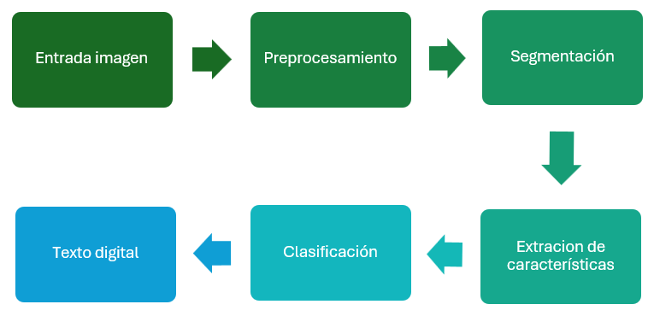
\includegraphics[width=0.7\textwidth]{Imagenes/procesoOCR.png}
    \caption{Flujo general del proceso OCR adaptado.}
    \label{fig:OCR}
\end{figure}
Adaptado de \cite{otsu1979threshold, smith2007overview}

Como se observa en la Figura \ref{fig:OCR}, el proceso comienza con la entrada de una imagen, que puede provenir de una fotografía o de un lienzo digital. Posteriormente, en la etapa de preprocesamiento, se realizan ajustes como conversión a escala de grises, binarización y eliminación de ruido, con el fin de mejorar la calidad visual para su análisis \cite{otsu1979threshold}. Estas técnicas permiten reducir variaciones no deseadas en la imagen, facilitando el reconocimiento posterior de los caracteres.

En la fase de segmentación, el sistema identifica y separa los caracteres individuales o grupos de caracteres dentro de la imagen. Este proceso resulta crítico, ya que una segmentación incorrecta puede afectar directamente la precisión del reconocimiento. A continuación, durante la extracción de características, se analizan propiedades específicas como contornos, formas y patrones estructurales que permiten diferenciar un carácter de otro.

Finalmente, en la etapa de clasificación, el sistema compara las características extraídas con modelos previamente entrenados para determinar a qué carácter corresponde cada patrón identificado, generando como resultado el texto digital final \cite{smith2007overview}. Esta etapa constituye el núcleo del sistema OCR, donde se realiza la toma de decisiones basada en modelos de reconocimiento.

Históricamente, los motores OCR se basaban en la comparación de plantillas estáticas y en la extracción de características geométricas como contornos y proyecciones de píxeles. Sin embargo, los enfoques contemporáneos han migrado hacia arquitecturas de aprendizaje profundo que logran tasas de reconocimiento significativamente superiores. En particular, las redes neuronales convolucionales (Convolutional Neural Networks, CNN por sus siglas en inglés) han demostrado ser especialmente efectivas en la extracción automática de rasgos visuales de caracteres sin requerir ingeniería manual de características \cite{lecun1998gradient}. Una evolución relevante es la arquitectura CRNN (Convolutional Recurrent Neural Network), que combina capas convolucionales para la extracción de características visuales con capas recurrentes para modelar dependencias secuenciales entre caracteres, permitiendo el reconocimiento de texto como una secuencia continua en lugar de caracteres aislados \cite{shi2017crnn}.

La etapa de preprocesamiento resulta determinante para la precisión del sistema. La binarización mediante el método de Otsu, que selecciona automáticamente un umbral óptimo de separación entre píxeles de fondo y trazo a partir del histograma de niveles de gris de la imagen, es una técnica ampliamente adoptada por su robustez ante variaciones de iluminación \cite{otsu1979threshold}. Complementariamente, técnicas de normalización del tamaño y corrección de inclinación (deskewing) contribuyen a reducir la variabilidad que enfrenta el clasificador.

La escritura manuscrita infantil presenta desafíos adicionales en comparación con texto impreso o escritura adulta. La irregularidad en el tamaño de letras, la variabilidad en el espaciado, los trazos incompletos y la presión inconsistente sobre la superficie de escritura introducen ruido que degrada el desempeño de los modelos \cite{graves2009connectionist}. Por ello, en aplicaciones educativas orientadas a estudiantes de educación primaria resulta necesario considerar márgenes de error más amplios y mecanismos de validación complementarios, tal como se establece en los requerimientos no funcionales del presente sistema (RNF-03).

En el caso de la escritura manuscrita, el OCR enfrenta desafíos adicionales debido a la variabilidad en estilos de letra, inclinación, tamaño y calidad del trazo. Estas variaciones incrementan la complejidad del reconocimiento y pueden generar errores si no se cuenta con modelos suficientemente robustos. Por ello, su integración en entornos educativos requiere considerar posibles márgenes de error y mecanismos complementarios de validación que permitan mejorar la confiabilidad del sistema.

El desarrollo reciente de sistemas de reconocimiento de escritura manuscrita ha evolucionado hacia el uso de modelos basados en aprendizaje profundo, particularmente redes neuronales recurrentes (RNN) y arquitecturas tipo Transformer, las cuales permiten modelar secuencias completas de texto sin requerir segmentación explícita de caracteres individuales. Este enfoque resulta especialmente relevante en escenarios donde la escritura presenta variaciones significativas, como es el caso de la escritura infantil, en la cual existen inconsistencias en tamaño, inclinación y separación entre caracteres \cite{shi2017crnn, huggingface2024trocr}.

Además, técnicas modernas como los mecanismos de atención han permitido mejorar la capacidad de los sistemas OCR para enfocarse en regiones relevantes de la imagen, incrementando la precisión en condiciones no ideales. Estas mejoras son particularmente útiles en aplicaciones educativas, donde las imágenes pueden presentar ruido, baja resolución o iluminación variable \cite{huggingface2024trocr}.

Por otra parte, la integración de modelos preentrenados ha permitido aprovechar grandes volúmenes de datos para mejorar el desempeño del reconocimiento, reduciendo la necesidad de entrenamiento desde cero y facilitando su adaptación a dominios específicos como la escritura manuscrita en educación básica \cite{goodfellow2016deep, google2024tessdata}. Este tipo de enfoques contribuye a mejorar la escalabilidad del sistema y su capacidad de adaptación a diferentes contextos.

No obstante, a pesar de estos avances, la precisión del OCR sigue dependiendo en gran medida de la calidad de la entrada, por lo que resulta fundamental garantizar condiciones adecuadas en la captura de la imagen y en el preprocesamiento, con el fin de maximizar el desempeño del sistema en aplicaciones reales.

\subsection{NLP}
El NLP es una rama de la inteligencia artificial que permite a los sistemas computacionales analizar, interpretar y generar lenguaje humano de manera automatizada \cite{jurafsky2023speech}. Esta disciplina combina conocimientos de lingüística, informática y aprendizaje automático para procesar texto y extraer información significativa, permitiendo transformar datos textuales en información útil para distintos tipos de aplicaciones.

En el ámbito educativo, el NLP se ha utilizado en aplicaciones como análisis de redacción, detección de errores ortográficos, evaluación automática de textos y generación de retroalimentación personalizada \cite{unesco2021ai}. Estas aplicaciones permiten apoyar el proceso de aprendizaje al proporcionar herramientas que facilitan la identificación de errores y la mejora continua del desempeño del estudiante.

A diferencia del OCR, que convierte imágenes en texto digital, el NLP trabaja directamente sobre el contenido textual, permitiendo su análisis lingüístico. Esta diferencia es fundamental dentro del sistema propuesto, ya que el OCR se encarga de la captura y digitalización del texto manuscrito, mientras que el NLP permite interpretar y analizar dicho contenido, estableciendo una relación directa entre ambas tecnologías.
El proceso general de detección de errores ortográficos mediante NLP puede representarse de forma conceptual en la Figura \ref{fig:NLP}.

\begin{figure}[H]
    \centering
    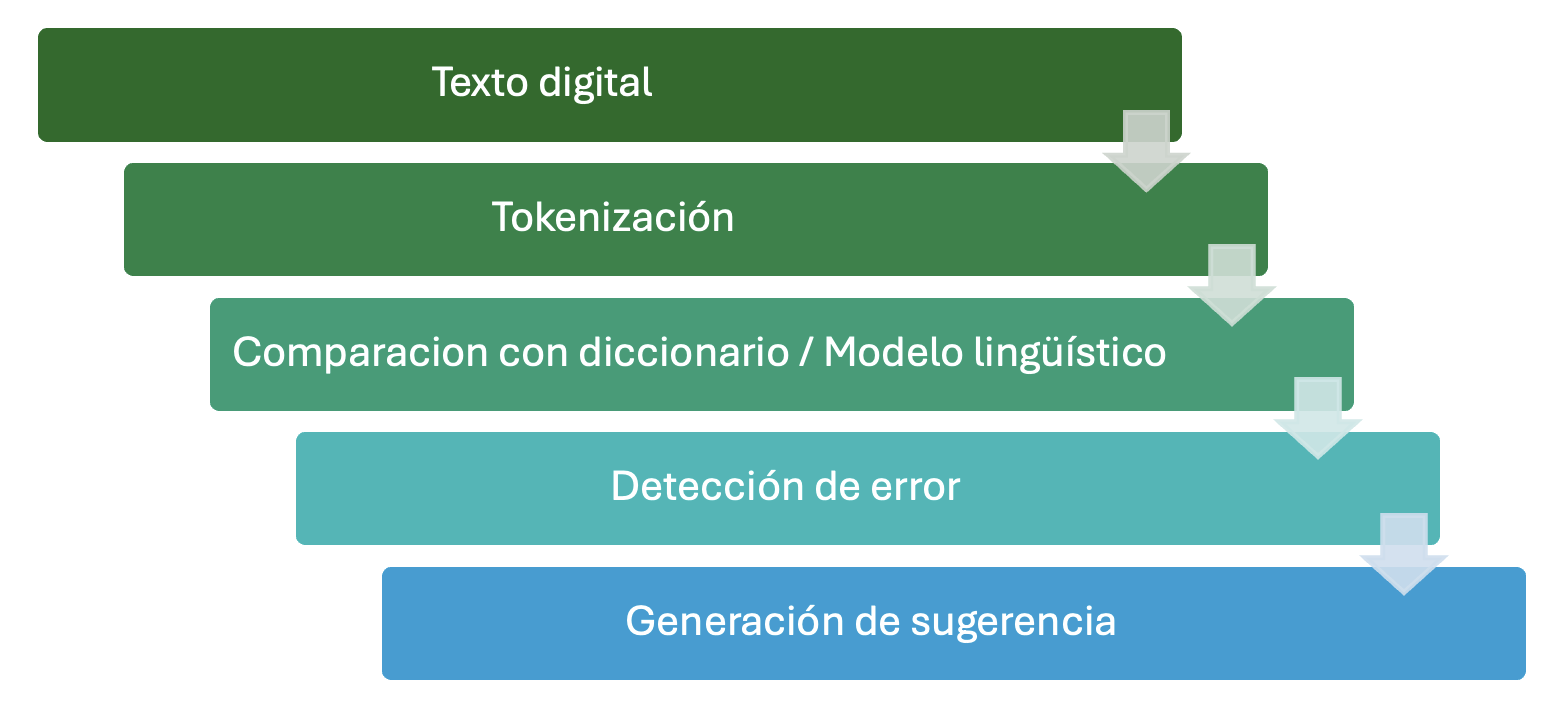
\includegraphics[width=0.7\textwidth]{Imagenes/procesoNLP.png}
    \caption{Flujo básico del proceso de corrección ortográfica mediante NLP. Elaboración con base en \cite{jurafsky2023speech}}
    \label{fig:NLP}
\end{figure}


Como se muestra en la Figura \ref{fig:NLP}, el procedimiento inicia con el texto digital previamente obtenido. Posteriormente, en la etapa de tokenización, el sistema divide el texto en unidades mínimas, generalmente palabras o tokens individuales, lo cual facilita su análisis individual y contextual dentro de la oración.

En la siguiente fase, cada token es comparado con un diccionario léxico o modelo lingüístico entrenado. Si una palabra no coincide con las entradas válidas, el sistema la identifica como posible error ortográfico. Para generar una sugerencia, pueden emplearse algoritmos de similitud como la distancia de Levenshtein o modelos estadísticos que calculan la probabilidad de ocurrencia de una palabra dentro de un contexto determinado \cite{jurafsky2023speech}. Este tipo de técnicas permite no solo detectar errores, sino también proponer alternativas adecuadas.

Este enfoque permite ofrecer retroalimentación automatizada en forma de sugerencias, lo cual resulta útil en entornos educativos cuando se busca apoyar el aprendizaje sin reemplazar la intervención del docente. No obstante, la precisión del sistema depende de la calidad del modelo lingüístico, del contexto del texto y de la claridad del contenido procesado.

La integración de NLP dentro del sistema propuesto permite complementar el análisis realizado por el OCR, cerrando el ciclo de procesamiento desde la captura del texto manuscrito hasta la generación de sugerencias ortográficas. Esta integración representa un enfoque más completo para el tratamiento de la información, combinando procesamiento visual y análisis lingüístico.

En los últimos años, el NLP ha experimentado avances significativos gracias al uso de modelos de representación distribuida del lenguaje, conocidos como embeddings, los cuales permiten capturar relaciones semánticas entre palabras en espacios vectoriales de alta dimensión. Estos modelos han demostrado ser efectivos para mejorar tareas de análisis lingüístico, incluyendo la corrección ortográfica contextual y la detección de errores en textos escritos \cite{ref34}.

Asimismo, el uso de modelos más avanzados basados en arquitecturas modernas ha permitido mejorar la comprensión del contexto dentro de una oración, lo que resulta especialmente útil en aplicaciones educativas donde los errores pueden depender no solo de la forma de la palabra, sino de su uso dentro de una estructura gramatical. Esto permite generar sugerencias más precisas y adaptadas al contexto real del usuario.

\subsection{Evaluación del trazo manuscrito}

El trazo manuscrito constituye un elemento relevante dentro del proceso de adquisición de la escritura en educación primaria. La legibilidad de un texto no depende únicamente de la ortografía correcta, sino también de factores visuales y espaciales que permiten interpretar adecuadamente el contenido escrito \cite{mikolov2013distributed, goodfellow2016deep}. Entre estos factores se encuentran la alineación sobre la línea base, la proporción del tamaño de las letras, el espaciado entre palabras y la uniformidad del trazo, los cuales influyen directamente en la claridad y comprensión del texto.

Diversos estudios sobre desarrollo de la escritura señalan que la evaluación de la letra manuscrita puede abordarse mediante parámetros observables que permitan identificar patrones de mejora o dificultad en los estudiantes \cite{berninger2010teaching, graham2010handwriting}. En contextos educativos tradicionales, esta evaluación es realizada por el docente de forma visual y cualitativa; sin embargo, con el apoyo de herramientas digitales es posible establecer métricas básicas que complementen dicha valoración, aportando un enfoque más objetivo al análisis del desempeño.

Desde una perspectiva computacional, algunos de estos parámetros pueden aproximarse mediante técnicas de análisis de imagen, tales como la medición de altura promedio de caracteres, la variación de inclinación o la separación entre segmentos gráficos \cite{marti2002iam, plamondon2000online}. Estas técnicas permiten cuantificar características del trazo que, de otra forma, serían evaluadas únicamente de manera subjetiva. Si bien estos indicadores no sustituyen la evaluación pedagógica, pueden ofrecer información cuantitativa útil para el seguimiento del progreso del estudiante a lo largo del tiempo.

Los principales parámetros considerados para la evaluación básica del trazo en el presente proyecto se describen en la Tabla \ref{tab:parametros_evaluacion}, donde se establecen tanto los criterios pedagógicos como sus posibles aproximaciones computacionales, permitiendo vincular la evaluación tradicional con el análisis automatizado.

\begin{table}[H]
\centering
\caption{Parámetros de evaluación del trazo manuscrito.}
\label{tab:parametros_evaluacion}
\renewcommand{\arraystretch}{1.5} % Da un poco más de espacio vertical entre las filas
\begin{tabular}{|>{\centering\arraybackslash}m{3cm}|>{\centering\arraybackslash}m{5.5cm}|>{\centering\arraybackslash}m{6cm}|}
\hline
\textbf{Parámetro} & \textbf{Descripción} & \textbf{Posible aproximación computacional} \\ \hline
Legibilidad & Claridad visual de los caracteres & Porcentaje de reconocimiento correcto por OCR \\ \hline
Alineación & Ubicación uniforme sobre línea base & Desviación vertical promedio \\ \hline
Tamaño & Proporción consistente de las letras & Altura media de caracteres \\ \hline
Espaciado & Separación adecuada entre letras & Distancia promedio entre segmentos \\ \hline
Uniformidad & Consistencia en forma y grosor del trazo & Variación en contornos detectados \\ \hline
\end{tabular}
\end{table}

Como se observa en la Tabla \ref{tab:parametros_evaluacion}, los parámetros seleccionados combinan criterios pedagógicos tradicionales con posibles métricas de análisis digital. Esta integración permite establecer un modelo básico de evaluación que apoye el seguimiento del desempeño del estudiante sin reemplazar la interpretación docente, sino más bien complementándola.

La incorporación de estos indicadores dentro del sistema propuesto busca complementar el análisis ortográfico realizado mediante NLP, ofreciendo una visión más integral del proceso de escritura. De esta manera, el sistema no solo evalúa la corrección del texto, sino también la calidad del trazo manuscrito, integrando así componentes visuales y lingüísticos dentro de una misma solución tecnológica.

\subsection{Arquitectura de la aplicación web}
El desarrollo de aplicaciones web modernas suele estructurarse bajo patrones de diseño que permiten organizar de manera eficiente los componentes del sistema. Uno de los modelos más utilizados es la arquitectura Modelo Vista Controlador(Model-View-Controller, MVC por sus siglas en inglés), la cual divide la aplicación en tres capas principales: modelo, vista y controlador \cite{ref33}.

En la Figura \ref{fig:MVC} se presenta el esquema general de la arquitectura MVC aplicada al sistema propuesto.

\begin{figure}[H]
    \centering
    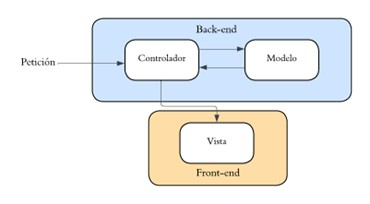
\includegraphics[width=0.7\textwidth]{Imagenes/MVC.jpg}
    \caption{Arquitectura Modelo-Vista-Controlador aplicada al sistema \cite{buschmann1996pattern}.}
    \label{fig:MVC}
\end{figure}

Como se observa en la Figura \ref{fig:MVC}, el flujo de operación inicia con una petición realizada desde el front-end. Esta solicitud es enviada al controlador, ubicado en el back-end, el cual actúa como intermediario entre la interfaz y la lógica del sistema. El controlador procesa la solicitud y se comunica con el modelo, donde se gestionan los datos y la lógica de negocio.

El modelo es responsable del almacenamiento de información, incluyendo usuarios, ejercicios realizados, resultados del OCR, análisis ortográfico mediante NLP y métricas asociadas a la calidad del trazo. Esta separación permite mantener organizada la lógica interna del sistema y facilita futuras modificaciones o ampliaciones.

Posteriormente, el controlador recibe la información procesada y genera una respuesta que es enviada a la vista, encargada de mostrar al usuario la retroalimentación correspondiente. Esta estructura modular favorece la mantenibilidad, escalabilidad y claridad del sistema \cite{ref37}.

Además, el despliegue del sistema en un servidor web funcional permite su acceso mediante navegador, garantizando un entorno controlado para la prueba piloto y la centralización de datos. La adopción del modelo MVC facilita la integración coherente de los módulos de OCR, NLP y evaluación del trazo dentro de una arquitectura estructurada.

\subsection{Experiencia de Usuario y Diseño de Interfaces Educativas}

El diseño de interfaces para aplicaciones educativas destinadas a niños de entre 8 y 10 años requiere un enfoque especializado que considere sus capacidades cognitivas, motoras y de alfabetización en desarrollo \cite{ref38}, \cite{ref39}. La Experiencia de Usuario (UX) en este rango de edad no solo busca la eficiencia en la ejecución de tareas, sino también fomentar el compromiso y minimizar la frustración durante el proceso de aprendizaje \cite{ref38}. Es vital entender que el diseño debe facilitar la transición entre lo digital y lo manual, preservando los beneficios cognitivos que la neurociencia atribuye al trazo físico sobre el teclado \cite{ref40}, \cite{ref41}.

\subsubsection{Consideraciones Cognitivas y Carga Visual}

A diferencia de los usuarios adultos, los estudiantes de tercer y cuarto grado poseen una capacidad limitada para procesar múltiples estímulos simultáneos, por lo que la interfaz debe minimizar la carga cognitiva mediante un diseño limpio y el uso de metáforas visuales claras \cite{ref39}. Esto implica la utilización de áreas de interacción amplias, botones de gran tamaño y tipografías legibles que cumplan con índices de lecturabilidad específicos para su nivel escolar, como el de Fernández-Huerta \cite{ref42}. Un diseño visualmente ordenado permite que el alumno mantenga la atención en el objetivo principal: la práctica de la escritura manuscrita \cite{ref38}.

\subsubsection{Arquitectura de Información y Navegación}
La navegación en sistemas educativos infantiles debe ser sencilla y preferiblemente plana, ya que las estructuras jerárquicas profundas suelen confundir a los usuarios jóvenes \cite{ref38}. Es recomendable que las funcionalidades principales sean accesibles con un mínimo de interacciones y que el uso de íconos representativos esté acompañado de etiquetas de texto sencillas que refuercen la autonomía del estudiante dentro de la plataforma \cite{ref39}. Además, la interfaz de captura debe ser lo suficientemente robusta para generar imágenes de alta calidad que permitan un procesamiento eficiente por parte de arquitecturas avanzadas de reconocimiento de texto como TrOCR \cite{ref43}.

\subsubsection{Retroalimentación y Sistemas de Respuesta}
La retroalimentación inmediata es un componente crítico para el aprendizaje guiado, especialmente en la detección de errores ortográficos y la evaluación de la calidad del trazo \cite{ref38}. El sistema debe proporcionar respuestas multisensoriales que informen al niño sobre sus aciertos y áreas de mejora de manera constructiva, reduciendo la ansiedad ante el error y promoviendo la persistencia en la actividad académica \cite{ref38}. Esta respuesta constante ayuda a consolidar las conexiones neuronales necesarias para el dominio de la escritura \cite{ref40}.

\subsubsection{Engagement y Gamificación}
Para mantener la motivación en tareas que requieren repetición, resulta beneficioso integrar elementos de gamificación como barras de progreso, insignias o recompensas visuales \cite{ref39}. El diseño debe equilibrar estos elementos lúdicos para que actúen como un refuerzo pedagógico efectivo sin convertirse en una distracción del proceso de aprendizaje central \cite{ref39}. El refuerzo positivo mediante herramientas digitales es una estrategia clave para evitar que el estudiante pierda el interés en el desarrollo de sus habilidades caligráficas tradicionales \cite{ref41}.

\section{Capítulo 3: Análisis}

En este capítulo se trabajará el análisis de los módulos de la aplicación para su correcto funcionamiento abarcando desde los límites y capacidades de la aplicación, así como los requerimientos, riesgos y mitigación de estos para tener una base sólida para el diseño y posterior desarrollo de nuestra solución.

\subsection{Alcance y Límites de la aplicación}

El propósito de este apartado es establecer de manera precisa el ámbito de desarrollo e implementación del proyecto. A continuación, se definen las capacidades operativas y el público objetivo que conforman el alcance del sistema, así como las restricciones técnicas, lingüísticas y de conectividad que delimitan su funcionamiento.

\subsubsection{Alcance de la aplicación web}

La aplicación web está dirigida exclusivamente a estudiantes de tercer y cuarto grado de educación primaria. La plataforma permitirá la recolección de textos manuscritos en letra de molde mediante la escritura directa en un lienzo en pantalla o a través de la carga de imágenes.

Una vez capturado, el texto será procesado mediante algoritmos de OCR para su digitalización, seguido por la intervención de un módulo de NLP encargado de analizar el contenido, detectar errores ortográficos y generar sugerencias automáticas de corrección.

Además, el sistema evaluará métricas cuantitativas del trazo manuscrito, considerando parámetros como la legibilidad, alineación, tamaño y espaciado.

\subsubsection{Límites de la aplicación web}

Las restricciones técnicas y operativas de la aplicación son en cuanto al estilo de escritura, el modelo de reconocimiento está estrictamente acotado al procesamiento de letra de molde (tipografía Century) \cite{ref40}, excluyendo la evaluación de letra cursiva u otras tipografías.

Respecto a la restricción lingüística, el análisis ortográfico y las sugerencias generadas se limitarán al nivel cognitivo y vocabulario correspondiente a los grados de tercero y cuarto de primaria.

En relación con el rol de la aplicación, el sistema funcionará exclusivamente como una herramienta de retroalimentación automatizada y complementaria, basada en un enfoque de aprendizaje ecléctico, sin sustituir la evaluación pedagógica integral del docente.

Finalmente, debido a su diseño basado en una arquitectura web cliente-servidor, existe una dependencia de conectividad, por lo que el funcionamiento de los módulos OCR y NLP requerirá una conexión activa a internet.


\subsection{Factibilidad}
 
El estudio de factibilidad es un instrumento que sirve para orientar la toma de decisiones en la evaluación de un proyecto. Se formula con base en información que tiene la menor incertidumbre posible para medir las posibilidades de éxito o fracaso, apoyándose en él se tomará la decisión de proceder o no con su implementación.
 
% ─────────────────────────────────────────────
\subsubsection{Factibilidad Técnica}
% ─────────────────────────────────────────────
 
La factibilidad técnica estudia la posibilidad tecnológica para que el proyecto pueda llevarse a cabo satisfactoriamente con el menor riesgo posible. Las herramientas tecnológicas se dividen en software y hardware.
 
\paragraph{Software}
 
El software es una parte esencial en la elaboración del proyecto, ya que con este se desarrollará la aplicación web y el servidor. Todas las herramientas seleccionadas tienen costo cero para el equipo, incluyendo GitHub en su plan gratuito, el cual cubre repositorios privados ilimitados, colaboradores ilimitados y 2{,}000 minutos mensuales de CI/CD, suficientes para un equipo de tres personas.
 
\begin{table}[H]
\centering
\caption{Herramientas de software para el desarrollo del proyecto.}
\label{tab:software}
\renewcommand{\arraystretch}{1.3}
\begin{tabularx}{\textwidth}{|l|X|l|r|r|}
\hline
\textbf{Herramienta} & \textbf{Uso en el proyecto} & \textbf{Tipo} & \textbf{Costo/mes} & \textbf{11 meses} \\
\hline
React / Next.js   & Front-End: panel tutor, panel alumno, lienzo digital  & Libre & \$0 & N/A \\
\hline
FastAPI (Python)  & Back-End: endpoints REST, lógica de negocio, JWT      & Libre & \$0 & N/A \\
\hline
SQL Server Express & Base de datos: tablas, triggers, vistas, restricciones & Libre & \$0 & N/A \\
\hline
Docker            & Contenedorización y despliegue                        & Libre & \$0 & N/A \\
\hline
VS Code           & Editor de código fuente                               & Libre & \$0 & N/A \\
\hline
GitHub (Free)     & Control de versiones, repos privados, CI/CD           & Libre & \$0 & N/A \\
\hline
GCP / AWS         & Hosting: prueba piloto en tier gratuito               & Libre & \$0 & N/A \\
\hline
\multicolumn{3}{|r|}{\textbf{Total}} & \multicolumn{2}{r|}{\textbf{\$0 MXN}} \\
\hline
\end{tabularx}
\end{table}
 
\paragraph{Hardware}
 
El hardware es fundamental para el desarrollo del proyecto. A continuación se presentan las especificaciones de los equipos de cómputo de cada integrante del equipo, los cuales serán utilizados durante todo el desarrollo.
 
\begin{table}[H]
\centering
\caption{Características de los equipos de cómputo y dispositivos de prueba.}
\label{tab:hardware}
\renewcommand{\arraystretch}{1.3}
\begin{tabularx}{\textwidth}{|X|X|c|c|c|r|}
\hline
\textbf{Equipo} & \textbf{Procesador} & \textbf{RAM} & \textbf{Almac.} & \textbf{SO} & \textbf{Valor ref. (MXN)} \\
\hline
Lenovo IdeaPad  & AMD Ryzen 7 & 16 GB & 512 GB SSD & Arch Linux & \$18,000 \\
\hline
MacBook Air     & Apple M1 & 8 GB & 256 GB SSD & macOS & \$28,000 \\
\hline
HP Spectre x360 & Intel Core i7 & 16 GB & 512 GB SSD & Windows 11 & \$25,000 \\
\hline
iPad / Tablets  & N/A & N/A & N/A & iPadOS/Android & \$10,000 \\
\hline
\multicolumn{5}{|r|}{\textbf{Total (valor de referencia — ya en posesión del equipo)}} & \textbf{\$81,000} \\
\hline
\end{tabularx}
\end{table}
 
Dadas las características de las herramientas tanto en software como en hardware, se puede observar que el proyecto puede llevarse a cabo correctamente. El stack tecnológico es coherente y moderno: React/Next.js cubre el front-end educativo, FastAPI con Python concentra la lógica de inteligencia artificial (OCR y NLP), y SQL Server garantiza integridad referencial con soporte a triggers y vistas. El Ryzen 7 y el M1 son los equipos más capaces para ejecutar los modelos localmente durante el desarrollo.
 
% ─────────────────────────────────────────────
\subsubsection{Factibilidad Operativa}
% ─────────────────────────────────────────────
 
La factibilidad operativa comprende una determinación de la probabilidad para que un proyecto se realice o funcione como se supone, considerando si se cuenta con el personal capacitado y los recursos humanos necesarios. Al realizar el análisis se calcula tanto el tiempo de esfuerzo como las horas dedicadas al sistema.
 
\begin{table}[H]
\centering
\caption{Resumen de días hábiles para el desarrollo del proyecto.}
\label{tab:dias}
\renewcommand{\arraystretch}{1.3}
\begin{tabularx}{\textwidth}{|l|r|r|r|r|r|r|}
\hline
\textbf{Mes} & \textbf{Días} & \textbf{Fin de semana} & \textbf{Días no laborales} & \textbf{Días hábiles} & \textbf{Hrs/día} & \textbf{Hrs totales} \\
\hline
Enero      & 31 & 9 & 1 & 21 & 4 & 84  \\
\hline
Febrero    & 28 & 8 & 1 & 19 & 4 & 76  \\
\hline
Marzo      & 31 & 8 & 1 & 22 & 4 & 88  \\
\hline
Abril      & 30 & 8 & 2 & 20 & 4 & 80  \\
\hline
Mayo       & 31 & 9 & 1 & 21 & 4 & 84  \\
\hline
Junio      & 30 & 8 & 0 & 22 & 4 & 88  \\
\hline
Julio      & 31 & 9 & 0 & 22 & 4 & 88  \\
\hline
Agosto     & 31 & 9 & 0 & 22 & 4 & 88  \\
\hline
Septiembre & 30 & 8 & 1 & 21 & 4 & 84  \\
\hline
\textbf{Total} & & & & \textbf{190} & & \textbf{760} \\
\hline
\end{tabularx}
\end{table}
 
Es necesaria la definición de roles en el desarrollo del proyecto para llevar una organización eficiente donde cada integrante desempeñe sus actividades sin generar retrasos. Dado que el equipo de trabajo cuenta con tres personas, es necesario que los integrantes desempeñen más de un rol a lo largo del proyecto.
 
\begin{table}[H]
\centering
\caption{Roles de trabajo del proyecto.}
\label{tab:roles}
\renewcommand{\arraystretch}{1.3}
\begin{tabularx}{\textwidth}{|l|X|r|}
\hline
\textbf{Rol} & \textbf{Descripción} & \textbf{Personas necesarias} \\
\hline
Líder de proyecto       & Encargado de la coordinación y planeación del proyecto.                                          & 1 \\
\hline
Analista / Arquitecto   & Realiza el análisis e diseño de la arquitectura del sistema y sus módulos.                       & 1 \\
\hline
Desarrollador Front-End & Desarrolla la interfaz de usuario con React/Next.js: paneles de tutor y alumno, lienzo digital.  & 1 \\
\hline
Desarrollador Back-End  & Implementa los endpoints REST con FastAPI, lógica de negocio, autenticación JWT y BCrypt.        & 1 \\
\hline
Especialista IA         & Integra y ajusta los módulos de OCR y NLP para análisis caligráfico y corrección ortográfica.    & 1 \\
\hline
Tester / QA             & Realiza las pruebas funcionales y de integración para validar el correcto funcionamiento.        & 1 \\
\hline
\end{tabularx}
\end{table}
 
A continuación se muestra la distribución del porcentaje de participación para cada rol y el promedio de días laborales correspondiente, tomando como base 190 días hábiles de desarrollo.
 
\begin{table}[H]
\centering
\caption{Porcentaje de participación de cada rol del proyecto.}
\label{tab:participacion}
\renewcommand{\arraystretch}{1.3}
\begin{tabularx}{\textwidth}{|X|r|r|}
\hline
\textbf{Rol} & \textbf{Porcentaje de participación} & \textbf{Días laborales} \\
\hline
Líder de proyecto       & 15\% & 28.5 días \\
\hline
Analista / Arquitecto   & 15\% & 28.5 días \\
\hline
Desarrollador Front-End & 20\% & 38.0 días \\
\hline
Desarrollador Back-End  & 20\% & 38.0 días \\
\hline
Especialista IA (OCR + NLP) & 20\% & 38.0 días \\
\hline
Tester / QA             & 10\% & 19.0 días \\
\hline
\end{tabularx}
\end{table}
 
La factibilidad operativa del proyecto se muestra positiva. Los días totales calculados son una estimación considerando una dedicación de 4 horas diarias promedio por integrante. Consideramos que el tiempo para el desarrollo tiene suficiente holgura siempre y cuando se sigan las actividades y los calendarios acordados, y se priorice la integración temprana entre módulos para detectar problemas antes de la prueba piloto con 25 alumnos.
 
% ─────────────────────────────────────────────
\subsubsection{Factibilidad Económica}
% ─────────────────────────────────────────────
 
Se toma en consideración el capital disponible para invertir en el desarrollo del proyecto. Se determina el presupuesto de costos de los recursos técnicos, humanos y materiales tanto para el desarrollo como para la implantación. El sueldo de referencia utilizado es de \$20{,}000 MXN mensuales por desarrollador de nivel junior a intermedio en México para el año 2025 \cite{occmundial2025salarios}.
 
En primer lugar, se presentan los costos de las herramientas de software, los cuales son en su totalidad de costo cero para el equipo de desarrollo.
 
\begin{table}[H]
\centering
\caption{Estimación de costos de herramientas de software.}
\label{tab:costos-software}
\renewcommand{\arraystretch}{1.3}
\begin{tabularx}{\textwidth}{|X|r|r|}
\hline
\textbf{Herramienta} & \textbf{Costo mensual (MXN)} & \textbf{Costo por 9 meses (MXN)} \\
\hline
React / Next.js, FastAPI, SQL Server Express, Docker, VS Code, Figma, Postman, GitHub Free, GCP/AWS (tier gratuito) & \$0 & \$0 \\
\hline
\textbf{Total} & \textbf{\$0} & \textbf{\$0} \\
\hline
\end{tabularx}
\end{table}
 
A continuación se presentan los costos de los servicios necesarios para llevar a cabo el proyecto.
 
\begin{table}[H]
\centering
\caption{Costos de servicios.}
\label{tab:servicios}
\renewcommand{\arraystretch}{1.3}
\begin{tabularx}{\textwidth}{|X|r|r|}
\hline
\textbf{Servicio} & \textbf{Costo por mes (MXN)} & \textbf{Costo por 9 meses (MXN)} \\
\hline
Electricidad e internet (3 integrantes × \$800) & \$2{,}400 & \$21{,}600 \\
\hline
Infraestructura en nube (GCP / AWS — tier gratuito en piloto) & \$0 & \$0 \\
\hline
\textbf{Total} & \textbf{\$2{,}400} & \textbf{\$21{,}600} \\
\hline
\end{tabularx}
\end{table}
 
Finalmente, en la Tabla \ref{tab:costos-total} se presenta el resumen de costos totales del proyecto.
 
\begin{table}[H]
\centering
\caption{Resumen de costos totales del proyecto.}
\label{tab:costos-total}
\renewcommand{\arraystretch}{1.3}
\begin{tabularx}{\textwidth}{|X|r|}
\hline
\textbf{Concepto} & \textbf{Costo total (MXN)} \\
\hline
Sueldos — costo comercial equivalente (3 personas × 9 meses × \$20{,}000) & \$540{,}000 \\
\hline
Equipo de cómputo (valor de referencia — ya en posesión del equipo)        & \$61{,}000 \\
\hline
Servicios (electricidad e internet, 9 meses)                               & \$21{,}600 \\
\hline
Herramientas de software                                                   & \$0        \\
\hline
Infraestructura en nube                                                    & \$0        \\
\hline
\textbf{Total}                                                             & \textbf{\$622{,}600} \\
\hline
\end{tabularx}
\end{table}
 
Con base en la tabla anterior, se puede concluir que el costo comercial equivalente del proyecto asciende a \$622{,}600 MXN. Sin embargo, al ser este un trabajo terminal, los sueldos (que representan el 86.7\% del total) son absorbidos por el propio equipo como parte de su formación académica, y el hardware ya se encuentra en posesión de los integrantes. El desembolso directo real del equipo se limita a los servicios básicos de electricidad e internet, estimados en \$21{,}600 MXN durante los 9 meses de desarrollo, siendo el resto de las herramientas completamente gratuitas.
\subsubsection{Factibilidad Legal}

La implementación del sistema requiere observar un conjunto de disposiciones jurídicas del ordenamiento mexicano que regulan directamente tres ámbitos: la protección de datos personales de menores de edad, los derechos de niñas, niños y adolescentes en entornos tecnológicos, y la propiedad intelectual del software académico. A continuación se analiza cada uno de estos marcos normativos y su aplicación concreta al sistema propuesto.

\subsubsection*{A. Protección de datos personales de menores de edad}
El tratamiento de los datos generados por el sistema — incluyendo muestras de escritura manuscrita, credenciales de acceso, resultados de análisis y métricas de desempeño — constituye tratamiento de datos personales en los términos de la Ley Federal de Protección de Datos Personales en Posesión de los Particulares (LFPDPPP), publicada originalmente en el Diario Oficial de la Federación el 5 de julio de 2010 y actualizada mediante la versión publicada el 20 de marzo de 2025, vigente a partir del 21 de marzo de 2025 \cite{lfpdppp2025}.

Dado que los usuarios finales son estudiantes de tercer y cuarto grado de educación primaria (entre 8 y 10 años de edad), se trata de datos personales de menores de edad, categoría que la ley somete a un régimen reforzado de protección. Los artículos específicos del ordenamiento que aplican al presente sistema son los siguientes:

\textbf{Artículo 7 (Consentimiento para menores de edad).} \\
La LFPDPPP establece que en el tratamiento de datos personales de menores de edad se deberá privilegiar el interés superior de la niña, el niño y el adolescente \cite{lfpdppp2025}. En concordancia con ello, la reforma de 2025 obliga expresamente a que el consentimiento para tratar datos de menores sea otorgado por padres, madres o tutores legales \cite{lfpdppp2025}. El sistema atiende este requerimiento mediante la figura del Tutor como actor principal del registro: únicamente el tutor autenticado puede dar de alta alumnos en la plataforma (RN-02), vinculando cada alumno a un responsable legal que actúa como representante en el tratamiento de sus datos (RN-03). Esto satisface el requisito de consentimiento informado, específico y libre exigido por la ley.

\textbf{Artículo 19 y 20 (Medidas de seguridad técnica, administrativa y física).} \\
La LFPDPPP obliga al responsable del tratamiento a implementar medidas de seguridad administrativas, técnicas y físicas que protejan los datos personales contra daño, pérdida, alteración, destrucción o acceso no autorizado \cite{lfpdppp2025}. El sistema da cumplimiento a este requerimiento mediante tres mecanismos: (1) autenticación basada en tokens JWT que impiden el acceso no autorizado a los datos de cada usuario según su rol; (2) almacenamiento de contraseñas mediante algoritmos de hash BCrypt (campo \texttt{contrasena\_cifrada} de tipo VARCHAR(255) en la tabla Usuarios); y (3) una arquitectura de separación de roles que garantiza que un alumno solo puede visualizar sus propios resultados (RN-25) y que únicamente el tutor responsable puede consultar y modificar los resultados de sus alumnos (RN-24).

\textbf{Derechos ARCO (Artículos 28--37).} \\
La ley reconoce a los titulares los derechos de Acceso, Rectificación, Cancelación y Oposición (ARCO) respecto de sus datos personales \cite{lfpdppp2025}. Para el ejercicio de estos derechos por parte de menores de edad, la ley dispone que deberá realizarse a través de su representante legal \cite{lfpdppp2025}. En el sistema, el tutor puede modificar los resultados de ejercicios de sus alumnos (RU-18) y el diseño contempla bajas lógicas en lugar de eliminación física de registros (RN-09), lo que permite la cancelación de datos sin comprometer la integridad referencial del sistema.

\textbf{Aviso de privacidad.} \\
El sistema deberá incorporar un aviso de privacidad accesible dentro de la interfaz, con lenguaje claro y adaptado al nivel educativo de los usuarios, informando sobre el responsable del tratamiento, las finalidades del uso de los datos, los mecanismos para el ejercicio de los derechos ARCO y el periodo de conservación de la información, en cumplimiento de los principios de licitud, información y proporcionalidad establecidos en la LFPDPPP \cite{lfpdppp2025}.

\subsubsection*{B. Derechos de niñas, niños y adolescentes en entornos tecnológicos}
La Ley General de los Derechos de Niñas, Niños y Adolescentes (LGDNNA), publicada en el Diario Oficial de la Federación el 4 de diciembre de 2014 y reformada por última vez el 27 de mayo de 2024, establece un catálogo de 20 derechos fundamentales aplicables a todas las personas menores de 18 años en territorio mexicano \cite{lgdnna2024}.

Dos artículos de esta ley resultan directamente relevantes para el presente proyecto:

\textbf{Artículo 13, fracción XX (Derecho de acceso a las Tecnologías de la Información y Comunicación).} \\
La LGDNNA reconoce expresamente el derecho de niñas, niños y adolescentes al acceso a las tecnologías de la información y comunicación, así como a los servicios de radiodifusión y telecomunicaciones, incluido el de banda ancha e internet, sin discriminación de ningún tipo o condición \cite{lgdnna2024}. El presente sistema se alinea con este derecho al constituir una herramienta educativa digital orientada a fortalecer competencias de escritura, ampliando las posibilidades de acceso a recursos tecnológicos dentro del entorno escolar de educación básica.

\textbf{Artículo 18 (Interés superior de la niñez como principio rector).} \\
La ley establece que en todas las medidas concernientes a niñas, niños y adolescentes se tomará en cuenta como consideración primordial su interés superior \cite{lgdnna2024}. Este principio se materializa en el diseño pedagógico del sistema: los ejercicios están basados en los programas de estudio de la SEP para tercer y cuarto grado, la retroalimentación automatizada es constructiva y no punitiva, y la interfaz está diseñada para minimizar la carga cognitiva y la frustración del estudiante.

\subsubsection*{C. Propiedad intelectual y licencias de software}
El desarrollo del sistema se enmarca en el régimen de Trabajo Terminal de la Escuela Superior de Cómputo (ESCOM) del Instituto Politécnico Nacional, cuyas normativas institucionales establecen que los derechos patrimoniales de los productos académicos generados corresponden a la institución, mientras que los autores conservan sus derechos morales \cite{escom_tt}.

Respecto al uso de herramientas de terceros, todas las tecnologías seleccionadas para el desarrollo cuentan con licencias compatibles con fines académicos y no comerciales:

\begin{itemize}
    \item \textbf{Tesseract OCR:} Licencia Apache 2.0, que permite uso, modificación y distribución sin restricciones para fines académicos.
    \item \textbf{FastAPI:} Licencia MIT, de uso libre sin condiciones.
    \item \textbf{React:} Licencia MIT.
    \item \textbf{Dataset Letras Alfabeto Español (Kaggle – Herrera, 2023):} Publicado bajo licencia Creative Commons, compatible con uso académico.
    \item \textbf{EMNIST:} Publicado por el NIST como dataset de acceso público para investigación.
\end{itemize}

El uso de estos componentes bajo sus respectivas licencias no genera obligaciones comerciales ni conflictos de propiedad intelectual con el marco institucional del proyecto.

\subsubsection*{D. Normatividad educativa}
El contenido pedagógico de los ejercicios y el análisis ortográfico del sistema se fundamentan en los programas de estudio de la Secretaría de Educación Pública (SEP) para educación básica — específicamente en los libros \textit{Nuestros Saberes} de tercer y cuarto grado (ciclo escolar 2025–2026) — lo que valida legalmente su pertinencia curricular dentro del sistema educativo nacional.

\subsubsection*{E. Síntesis de cumplimiento normativo}
En la Tabla \ref{tab:cumplimiento_normativo} se presenta un resumen del cumplimiento normativo del sistema respecto a las disposiciones legales identificadas como aplicables.

\begin{table}[H]
\centering
\caption{Síntesis de cumplimiento normativo del sistema.}
\label{tab:cumplimiento_normativo}
\renewcommand{\arraystretch}{1.5}
\begin{tabular}{|>{\centering\arraybackslash}m{3.5cm}|>{\centering\arraybackslash}m{4.5cm}|>{\centering\arraybackslash}m{7cm}|}
\hline
\textbf{Marco normativo} & \textbf{Artículo(s) aplicable(s)} & \textbf{Mecanismo de cumplimiento en el sistema} \\ \hline
LFPDPPP (2025) & Art. 7 --- Consentimiento de menores & Registro de alumnos exclusivamente por el tutor responsable (RN-02, RN-03) \\ \hline
LFPDPPP (2025) & Arts. 19--20 --- Seguridad técnica & JWT, BCrypt, separación de roles (RN-24, RN-25) \\ \hline
LFPDPPP (2025) & Arts. 28--37 --- Derechos ARCO & Modificación de resultados por tutor (RU-18), baja lógica (RN-09) \\ \hline
LGDNNA (2024) & Art. 13 fracc. XX --- Acceso a TIC & Herramienta digital educativa de acceso supervisado \\ \hline
LGDNNA (2024) & Art. 18 --- Interés superior & Diseño pedagógico basado en programas SEP, retroalimentación constructiva \\ \hline
Reglamento ESCOM-IPN & Propiedad intelectual académica & Derechos patrimoniales al IPN, derechos morales a los autores \\ \hline
Licencias de software de terceros & Apache 2.0, MIT, CC & Uso académico sin restricciones en todos los componentes \\ \hline
Programas SEP 3.$^{\circ}$ y 4.$^{\circ}$ grado & Plan de Estudios 2017 / Nuestros Saberes 2024 & Ejercicios diseñados con base en contenidos curriculares oficiales \\ \hline
\end{tabular}
\end{table}

En razón de lo anterior, el proyecto se considera legalmente factible. El diseño del sistema contempla de forma explícita los requerimientos normativos vigentes en materia de protección de datos de menores, derechos digitales de la infancia y propiedad intelectual académica, sin que ninguna disposición identificada represente un impedimento para su desarrollo o despliegue en un entorno educativo supervisado.

\clearpage % Para asegurar que la tabla no se desborde a la siguiente sección
\subsection{Requerimientos del usuario.}

En esta sección se describen los requerimientos del usuario, los cuales representan las expectativas y servicios que esperan los usuarios finales de la aplicación web. Estos requerimientos han sido identificados con base al análisis del problema, con el objetivo de propiciar que la solución desarrollada sea útil.

Los requerimientos del usuario se definen, de manera general, qué debe hacer la aplicación web desde la perspectiva del usuario en un lenguaje natural, sin entregar detalles técnicos de implementación. Estos servirán como base para la definición de requerimientos funcionales y no funcionales. 

\begin{tabularx}{\textwidth}{|>{\centering\arraybackslash}m{2cm}|m{3.6cm}|Y|>{\centering\arraybackslash}m{2.0cm}|}
\caption{Requerimientos del usuario.}
\label{tab:ru} \\

\hline
\textbf{ID} & \textbf{Nombre} & \textbf{Descripción} & \textbf{Prioridad} \\
\hline
\endfirsthead

\hline
\textbf{ID} & \textbf{Nombre} & \textbf{Descripción} & \textbf{Prioridad} \\
\hline
\endhead

\hline
\endfoot

% RU-01
RU-01 &
Registro de usuarios. &
La aplicación web debe permitir el registro de usuarios. El tutor se registra de forma autónoma, mientras que los alumnos son registrados por el tutor, asociándolos a su grado y grupo. &
Alta \\
\hline

% RU-02
RU-02 &
Autenticación de usuario. &
El usuario debe poder autenticarse en la aplicación web para acceder a sus funcionalidades de acuerdo con su rol. &
Alta \\
\hline

% RU-03
RU-03 &
Visualización de estado de alumnos. &
El tutor debe poder visualizar el estado de desempeño de sus alumnos, clasificándolos como bajo desempeño, desempeño regular y desempeño de excelencia, con el fin de identificar su progreso. &
Alta \\
\hline

% RU-04
RU-04 &
Clasificación de alumnos. &
La aplicación web debe mostrar un gráfico con la cantidad de alumnos clasificados según su nivel de desempeño (bajo, regular y excelencia), actualizándose conforme a los resultados obtenidos en ortografía y legibilidad. &
Media \\
\hline

% RU-05
RU-05 &
Visualización de ejercicios. &
La aplicación web debe permitir observar los ejercicios disponibles. &
Alta \\
\hline

% RU-06
RU-06 &
Activación de ejercicios. &
El tutor debe poder activar ejercicios a su elección, estableciendo una fecha límite de entrega cuando lo considere necesario. &
Alta \\
\hline

% RU-07
RU-07 &
Visualización de ejercicios seleccionados. &
La aplicación web debe mostrar los ejercicios seleccionados por el tutor y su fecha límite de entrega. &
Media \\
\hline

% RU-08
RU-08 &
Visualización de ejercicios pendientes. &
El alumno debe poder observar los ejercicios asignados y su fecha límite de entrega, para una correcta organización y cumplimiento de sus actividades en tiempo. &
Alta \\
\hline

% RU-09
RU-09 &
Visualización de ejercicios vencidos por tutor. &
La aplicación web debe permitir al tutor consultar los ejercicios cuya fecha límite ha expirado, para poder extender el plazo de entrega si lo considera necesario. &
Media \\
\hline

% RU-10
RU-10 &
Visualización de ejercicios vencidos por alumno. &
El alumno debe poder observar los ejercicios que no completó a tiempo, para conocer su estado y saber si el tutor ya habilitó su entrega. &
Media \\
\hline

% RU-11
RU-11 &
Realizar intento de ejercicios pendientes. &
El alumno debe poder realizar el ejercicio seleccionado por el tutor en una vista de captura de escritura. &
Alta \\
\hline

% RU-12
RU-12 &
Escritura digital en lienzo. &
El alumno debe poder escribir directamente sobre un lienzo digital, contando con herramientas de goma y deshacer para corregir su trazo, con el fin de realizar el ejercicio de escritura manuscrita desde el dispositivo. &
Alta \\
\hline

% RU-13
RU-13 &
Carga de fotografía como alternativa. &
El alumno debe poder subir una fotografía de su escritura manuscrita en papel como alternativa al lienzo digital, para adaptarse a distintas condiciones de acceso. &
Alta \\
\hline

% RU-14
RU-14 &
Envío del ejercicio para revisión. &
El alumno debe poder enviar su ejercicio a la aplicación web para que sea analizado, una vez que considere que su escritura está lista. &
Alta \\
\hline

% RU-15
RU-15 &
Visualización de ejercicios completados. &
El alumno debe poder observar los ejercicios completados, así como sus resultados de escritura. &
Media \\
\hline

% RU-16
RU-16 &
Visualización de ejercicios completados por alumno. &
La aplicación web debe permitir al tutor observar las actividades realizadas por cada alumno, incluyendo sus resultados. &
Media \\
\hline

% RU-17
RU-17 &
Modificación de resultados. &
El tutor debe poder modificar los resultados de un ejercicio realizado por el alumno, en caso de no estar de acuerdo con el análisis ortográfico y caligráfico. &
Baja \\
\hline

% RU-18
RU-18 &
Visualización de actividades sugeridas. &
El alumno debe poder observar las actividades sugeridas por la aplicación web, correspondientes a sus análisis ortográficos y caligráficos. &
Media \\
\hline

% RU-19
RU-19 &
Realizar actividades sugeridas. &
El alumno debe poder realizar las actividades sugeridas por la aplicación web, para trabajar en la mejora de los aspectos detectados en su escritura. &
Media \\
\hline

\end{tabularx}

%------- Reglas de negocio

\subsection{Reglas de negocio}

\begin{tabularx}{\textwidth}{|>{\centering\arraybackslash}m{2cm}|m{3.6cm}|Y|>{\centering\arraybackslash}m{2.0cm}|}
\caption{Reglas de negocio.}
\label{tab:rn} \\

\hline
\textbf{ID} & \textbf{Nombre} & \textbf{Descripción}  \\
\hline
\endfirsthead

\hline
\textbf{ID} & \textbf{Nombre} & \textbf{Descripción}  \\
\hline
\endhead

\hline
\endfoot

RN-01 & Registro de tutores &
Todo usuario que actúe como tutor debe estar registrado en el sistema con el rol de tutor. \\ \hline

RN-02 & Registro de alumnos &
Todo alumno debe estar registrado en el sistema para poder realizar intentos y consultar resultados. \\ \hline

RN-03 & Tutor único por alumno &
Cada alumno debe tener exactamente un tutor asignado. \\ \hline

RN-04 & Tutor con múltiples alumnos &
Un tutor puede estar asociado a uno o más alumnos. \\ \hline

RN-05 & Correo obligatorio para tutores &
Todo tutor debe proporcionar un correo electrónico válido. \\ \hline

RN-06 & Integridad tutor--alumno &
No se permite registrar un alumno sin asignarlo a un tutor existente. \\ \hline

RN-07 & Persistencia de datos &
La información de alumnos, tutores, intentos y resultados debe conservarse de manera persistente. \\ \hline

RN-08 & Baja lógica de usuarios &
La eliminación de usuarios debe realizarse de forma lógica (cambio de estado) y no física. \\ \hline

RN-09 & Asociación de intento &
Cada intento debe estar asociado a un único alumno y a un único ejercicio. \\ \hline

RN-10 & Evidencia obligatoria del intento &
Cada intento debe incluir una evidencia asociada. \\ \hline

RN-11 & Registro de fecha y hora &
Cada intento debe almacenar la fecha y hora en que fue enviado. \\ \hline

RN-12 & Análisis caligráfico único &
Cada intento debe generar exactamente un análisis caligráfico. \\ \hline

RN-13 & Análisis ortográfico único &
Cada intento debe generar exactamente un análisis ortográfico. \\ \hline

RN-14 & Generación automática de análisis &
Los análisis del intento deben generarse automáticamente a partir del contenido del intento. \\ \hline

RN-15 & Métricas caligráficas mínimas &
El análisis caligráfico debe evaluar, como mínimo: alineación, tamaño, inclinación y espaciado. \\ \hline

RN-16 & Rango de métricas caligráficas &
Cada métrica caligráfica debe tener un valor dentro del rango de 0 a 10. \\ \hline

RN-17 & Observaciones del análisis &
El análisis caligráfico puede incluir observaciones adicionales generadas por el tutor. \\ \hline

RN-18 & Detección de errores ortográficos &
El análisis ortográfico debe detectar errores ortográficos en el texto del intento. \\ \hline

RN-19 & Conteo de errores &
El sistema debe almacenar el conteo total de errores ortográficos detectados por intento. \\ \hline

RN-20 & Sugerencias de corrección &
El sistema debe generar sugerencias de corrección ortográfica. \\ \hline

RN-21 & Puntuación ortográfica &
El análisis ortográfico debe asignar una puntuación ortográfica basada en los errores detectados dentro del rango de 0 a 10. \\ \hline

RN-22 & Historial y progreso del alumno &
El historial y el progreso del alumno deben generarse a partir de los datos de análisis de sus intentos. \\ \hline

RN-23 & Consulta por tutor &
Un tutor puede consultar los resultados de los alumnos a su cargo. \\ \hline

RN-24 & Modificación por tutor &
Un tutor puede modificar los resultados de los alumnos a su cargo únicamente si la política del sistema lo permite y queda registro del cambio. \\ \hline

RN-25 & Consulta por alumno &
Un alumno solo puede visualizar sus propios resultados. \\ \hline

RN-26 & Condición para ejercicio correctivo &
Un ejercicio correctivo automático solo puede generarse si el conteo de errores del intento es menor que 5. \\ \hline

RN-27 & Disponibilidad de impresión &
Todo ejercicio debe poder renderizarse para visualización e impresión/exportación. \\ \hline

\end{tabularx}

%---------- Casos de uso

\subsection{Modelado de casos de uso}
El modelado de casos de uso se utiliza ampliamente para apoyar la adquisición de requerimientos. Un caso de uso puede tomarse como un simple escenario que describa lo que espera el usuario de un sistema.

Cada caso de uso representa una tarea discreta que implica interacción externa con un sistema. En su forma más simple, un caso de uso se muestra como una elipse, con los actores que intervienen en el caso de uso representados como figuras humanas \cite{sommerville2015software}. 

\subsubsection{Diagrama de casos de uso }

\begin{figure}[H]
  \centering
  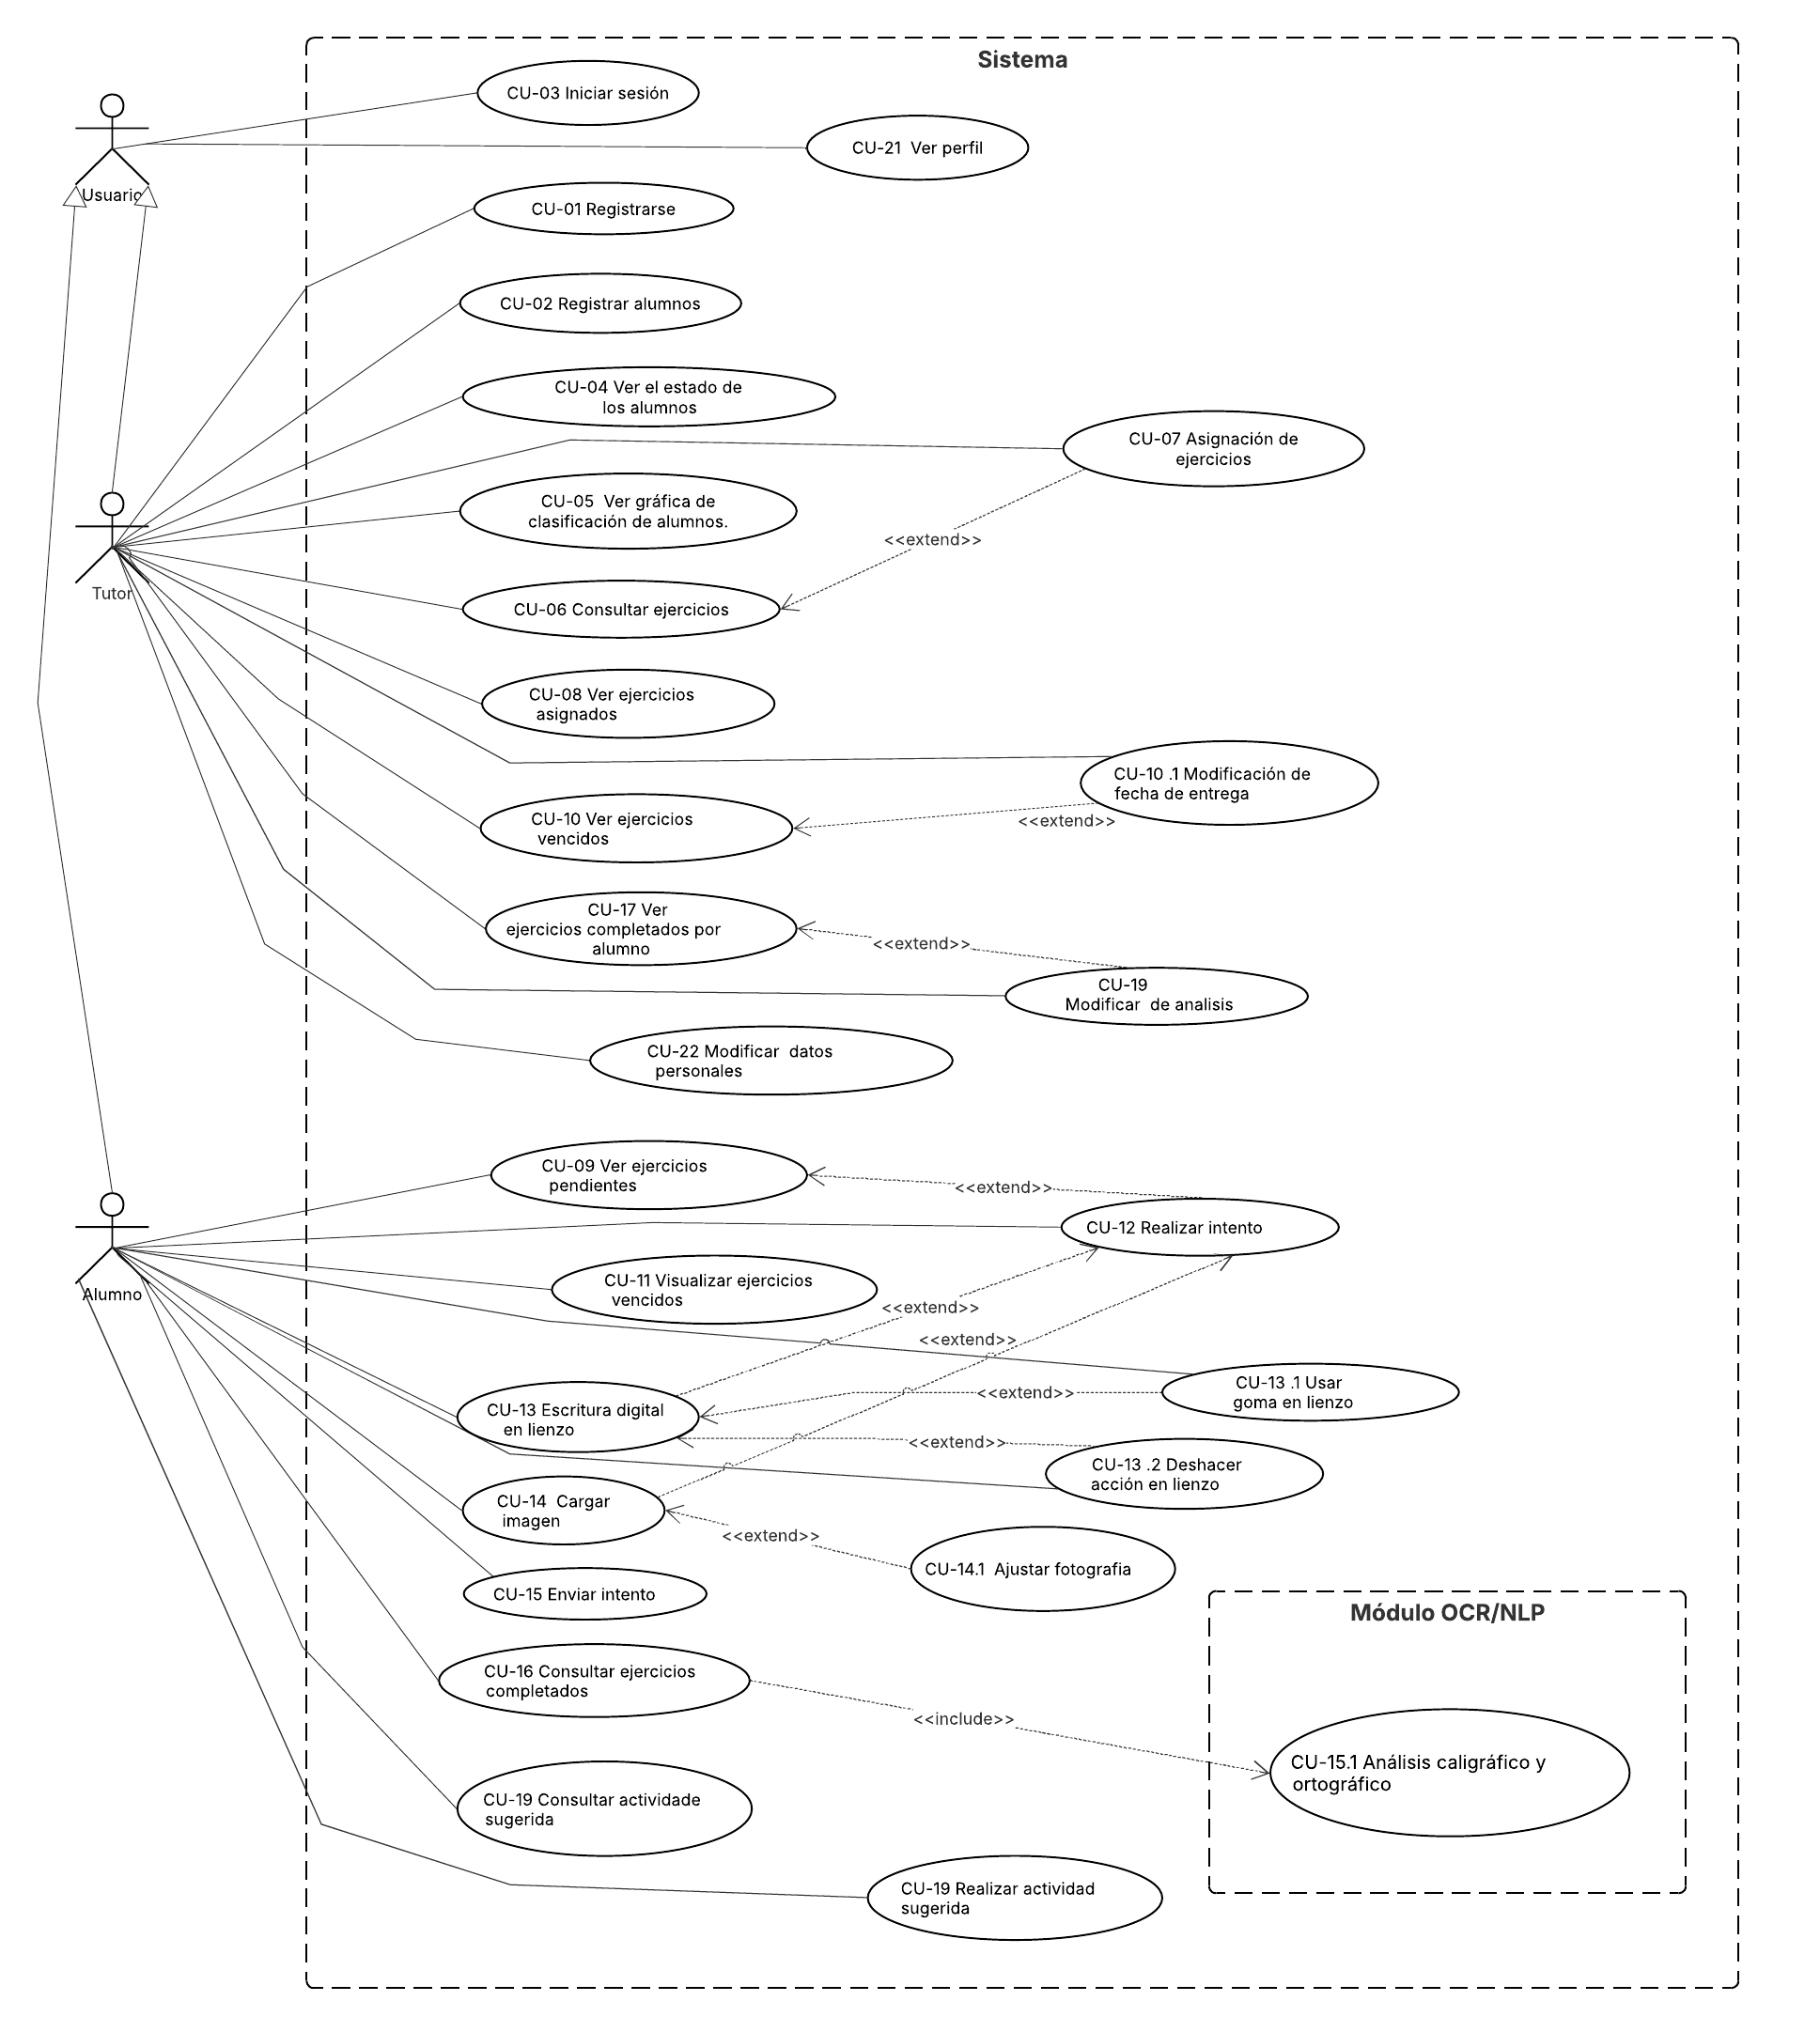
\includegraphics[height=0.82\textheight,keepaspectratio]{Imagenes/DiagramaCU-3.png}
  \caption{Diagrama de casos de uso}
\end{figure}

\subsubsection{Especificación de los casos de uso}

\begin{longtable}{|p{4cm}|p{11cm}|}
\caption{Tabla de especificación CU-01}
\label{tab:cu01} \\

\hline
\multicolumn{2}{|c|}{\textbf{CU-01 Registro de tutor}} \\
\hline
\endfirsthead

\hline
\multicolumn{2}{|c|}{\textbf{CU-01 Registro de tutor}} \\
\hline
\endhead

\hline
\endfoot

Actor & Tutor \\
\hline

Descripción & El tutor ingresa sus datos personales en el formulario de la aplicación web para crear su cuenta y acceder a sus funcionalidades. \\
\hline

Datos & Nombre, apellido paterno, nombre de usuario, correo electrónico, contraseña. \\
\hline

Estímulo & El tutor ingresa a la vista de registro, ingresa sus datos en el formulario y los envía. \\
\hline

Respuesta & La aplicación web valida los datos, crea la cuenta del tutor y le permite acceder a las funcionalidades del tutor. \\
\hline

Comentarios & El correo electrónico y nombre de usuario debe ser único en la aplicación web. \\
\hline

\end{longtable}

\begin{longtable}{|p{4cm}|p{11cm}|}
\caption{Tabla de especificación CU-02}
\label{tab:cu02} \\

\hline
\multicolumn{2}{|c|}{\textbf{CU-02 Registrar alumno}} \\
\hline
\endfirsthead

\hline
\multicolumn{2}{|c|}{\textbf{CU-02 Registrar alumno}} \\
\hline
\endhead

\hline
\endfoot

Actor & Tutor \\
\hline
Descripción & El tutor registra a un alumno en la aplicación web, ingresando sus datos e indicando el grado y grupo al que pertenece. \\
\hline
Datos & Nombre, apellido paterno, apellido materno, nombre de usuario, contraseña, grado y grupo. \\
\hline
Estímulo & El tutor, ya autenticado, ingresa a la vista ``Alumnos'', captura los datos en el formulario ``Alta de alumno'' y los envía. \\
\hline
Respuesta & La aplicación web registra los datos del alumno y lo asocia con el tutor responsable. \\
\hline
Comentarios & El nombre de usuario del alumno debe ser único. Solo tutores registrados pueden dar de alta alumnos. \\
\hline

\end{longtable}

%------------------------------------------------------

\begin{longtable}{|p{4cm}|p{11cm}|}
\caption{Tabla de especificación CU-03}
\label{tab:cu03} \\

\hline
\multicolumn{2}{|c|}{\textbf{CU-03 Iniciar sesión}} \\
\hline
\endfirsthead

\hline
\multicolumn{2}{|c|}{\textbf{CU-03 Iniciar sesión}} \\
\hline
\endhead

\hline
\endfoot

Actor & Tutor, Alumno \\
\hline
Descripción & El usuario ingresa sus credenciales para autenticarse y acceder a las funcionalidades según su rol. \\
\hline
Datos & Nombre de usuario y contraseña. \\
\hline
Estímulo & El usuario accede a la aplicación e ingresa sus credenciales en el formulario de inicio de sesión. \\
\hline
Respuesta & La aplicación valida las credenciales, identifica el rol y redirige a la vista correspondiente. \\
\hline
Comentarios & Si las credenciales son incorrectas, se muestra un mensaje de error. \\
\hline

\end{longtable}

%------------------------------------------------------

\begin{longtable}{|p{4cm}|p{11cm}|}
\caption{Tabla de especificación CU-04}
\label{tab:cu04} \\

\hline
\multicolumn{2}{|c|}{\textbf{CU-04 Ver el estado de los alumnos}} \\
\hline
\endfirsthead

\hline
\multicolumn{2}{|c|}{\textbf{CU-04 Ver el estado de los alumnos}} \\
\hline
\endhead

\hline
\endfoot

Actor & Tutor \\
\hline
Descripción & El tutor consulta el estado de desempeño de sus alumnos clasificados como bajo, regular y excelencia. \\
\hline
Datos & Lista de alumnos clasificados y métricas de progreso. \\
\hline
Estímulo & El tutor autenticado accede a su panel principal. \\
\hline
Respuesta & La aplicación muestra la lista de alumnos agrupados por categoría de desempeño. \\
\hline
Comentarios & Solo se muestran alumnos asociados al tutor autenticado. \\
\hline

\end{longtable}

%------------------------------------------------------

\begin{longtable}{|p{4cm}|p{11cm}|}
\caption{Tabla de especificación CU-05}
\label{tab:cu05} \\

\hline
\multicolumn{2}{|c|}{\textbf{CU-05 Ver gráfica de clasificación de alumnos}} \\
\hline
\endfirsthead

\hline
\multicolumn{2}{|c|}{\textbf{CU-05 er gráfica de clasificación de alumnos}} \\
\hline
\endhead

\hline
\endfoot

Actor & Tutor \\
\hline
Descripción & La aplicación presenta al tutor un gráfico con la distribución de alumnos según su nivel de desempeño. \\
\hline
Datos & Cantidad de alumnos en bajo, regular y excelencia. \\
\hline
Estímulo & El tutor accede al panel principal donde se muestra el gráfico. \\
\hline
Respuesta & La aplicación genera y actualiza dinámicamente el gráfico. \\
\hline
Comentarios & Puede mostrarse mediante gráfica de barras o anillo. \\
\hline

\end{longtable}

%------------------------------------------------------

\begin{longtable}{|p{4cm}|p{11cm}|}
\caption{Tabla de especificación CU-06}
\label{tab:cu06} \\

\hline
\multicolumn{2}{|c|}{\textbf{CU-06 Consultar ejercicios}} \\
\hline
\endfirsthead

\hline
\multicolumn{2}{|c|}{\textbf{CU-06 Consultar ejercicios}} \\
\hline
\endhead

\hline
\endfoot

Actor & Tutor \\
\hline
Descripción & La aplicación presenta al tutor el catálogo de ejercicios disponibles para asignar. \\
\hline
Datos & Nombre, descripción y contenido base del ejercicio. \\
\hline
Estímulo & El tutor accede a la sección de ejercicios. \\
\hline
Respuesta & La aplicación despliega el catálogo de ejercicios disponibles. \\
\hline
Comentarios & El tutor no crea ejercicios, solo los consulta y selecciona. \\
\hline

\end{longtable}

%------------------------------------------------------

\begin{longtable}{|p{4cm}|p{11cm}|}
\caption{Tabla de especificación CU-07}
\label{tab:cu07} \\

\hline
\multicolumn{2}{|c|}{\textbf{CU-07 Asignación de ejercicios}} \\
\hline
\endfirsthead

\hline
\multicolumn{2}{|c|}{\textbf{CU-07 Asignación de ejercicios}} \\
\hline
\endhead

\hline
\endfoot

Actor & Tutor \\
\hline
Descripción & El tutor selecciona uno o más ejercicios del catálogo y los activa para sus alumnos. \\
\hline
Datos & Ejercicios seleccionados, fecha límite opcional. \\
\hline
Estímulo & El tutor selecciona ejercicios y confirma la activación. \\
\hline
Respuesta & La aplicación registra los ejercicios activos y los publica a los alumnos. \\
\hline
Comentarios & La fecha límite es opcional. \\
\hline

\end{longtable}

%------------------------------------------------------

\begin{longtable}{|p{4cm}|p{11cm}|}
\caption{Tabla de especificación CU-08}
\label{tab:cu08} \\

\hline
\multicolumn{2}{|c|}{\textbf{CU-08 Ver ejercicios asignados}} \\
\hline
\endfirsthead

\hline
\multicolumn{2}{|c|}{\textbf{CU-08 Ver ejercicios asignados}} \\
\hline
\endhead

\hline
\endfoot

Actor & Tutor \\
\hline
Descripción & El tutor consulta la lista de ejercicios activados y sus fechas límite. \\
\hline
Datos & Ejercicios activos y fecha de entrega. \\
\hline
Estímulo & El tutor accede al módulo de ejercicios asignados. \\
\hline
Respuesta & La aplicación muestra los ejercicios seleccionados por el tutor. \\
\hline
Comentarios & Debe distinguir ejercicios con y sin fecha límite. \\
\hline

\end{longtable}

%------------------------------------------------------

\begin{longtable}{|p{4cm}|p{11cm}|}
\caption{Tabla de especificación CU-09}
\label{tab:cu09} \\

\hline
\multicolumn{2}{|c|}{\textbf{CU-09 Ver ejercicios pendientes}} \\
\hline
\endfirsthead

\hline
\multicolumn{2}{|c|}{\textbf{CU-09 Ver ejercicios pendientes}} \\
\hline
\endhead

\hline
\endfoot

Actor & Alumno \\
\hline
Descripción & El alumno consulta los ejercicios pendientes asignados por el tutor. \\
\hline
Datos & Nombre del ejercicio, descripción y fecha límite. \\
\hline
Estímulo & El alumno accede a la sección de ejercicios pendientes. \\
\hline
Respuesta & La aplicación muestra la lista de ejercicios activos no completados. \\
\hline
Comentarios & Solo se muestran ejercicios vigentes. \\
\hline

\end{longtable}

% CU-10
\begin{longtable}{|p{4cm}|p{11cm}|}
\caption{Tabla de especificación CU-10}
\label{tab:cu10} \\

\hline
\multicolumn{2}{|c|}{\textbf{CU-10 Visualización de ejercicios vencidos}} \\
\hline
\endfirsthead

\hline
\multicolumn{2}{|c|}{\textbf{CU-10 Visualización de ejercicios vencidos}} \\
\hline
\endhead

\hline
\endfoot

Actor & Tutor \\
\hline

Descripción & El tutor consulta la lista de ejercicios cuya fecha límite de entrega ha expirado, con el fin de decidir si extiende el plazo para uno o más de ellos. \\
\hline

Datos & Ejercicios seleccionados vencidos, fecha de entrega. \\
\hline

Estímulo & El tutor accede a la sección de ejercicios desde su panel de gestión y filtra los ejercicios seleccionados. \\
\hline

Respuesta & La aplicación web muestra únicamente los ejercicios activados por ese tutor, indicando para cada uno su fecha límite de entrega si fue establecida. \\
\hline

Comentarios & Debe distinguirse visualmente si un ejercicio fue seleccionado y ya está vencido. \\
\hline

\end{longtable}


% CU-11
\begin{longtable}{|p{4cm}|p{11cm}|}
\caption{Tabla de especificación CU-11}
\label{tab:cu11} \\

\hline
\multicolumn{2}{|c|}{\textbf{CU-11 Visualización de ejercicios vencidos}} \\
\hline
\endfirsthead

\hline
\multicolumn{2}{|c|}{\textbf{CU-11 Visualización de ejercicios vencidos}} \\
\hline
\endhead

\hline
\endfoot

Actor & Alumno \\
\hline

Descripción & El alumno consulta los ejercicios vencidos y no completados para conocer su estado y verificar si el tutor ha extendido el plazo de entrega. \\
\hline

Datos & Lista de ejercicios vencidos con nombre, fecha límite original y estado de habilitación por parte del tutor. \\
\hline

Estímulo & El alumno, autenticado en la aplicación web, accede a la sección de ejercicios vencidos desde su panel principal. \\
\hline

Respuesta & La aplicación web muestra los ejercicios no completados a tiempo, indicando si el tutor ha habilitado o no su entrega posterior. \\
\hline

Comentarios & Se debe distinguir entre ejercicios vencidos sin extensión y aquellos que el tutor habilitó nuevamente. \\
\hline

\end{longtable}


% CU-12
\begin{longtable}{|p{4cm}|p{11cm}|}
\caption{Tabla de especificación CU-12}
\label{tab:cu12} \\

\hline
\multicolumn{2}{|c|}{\textbf{CU-12 Realizar intento de ejercicio pendiente}} \\
\hline
\endfirsthead

\hline
\multicolumn{2}{|c|}{\textbf{CU-12 Realizar intento de ejercicio pendiente}} \\
\hline
\endhead

\hline
\endfoot

Actor & Alumno \\
\hline

Descripción & El alumno selecciona un ejercicio pendiente asignado por el tutor y accede a la vista de captura de escritura para realizarlo. \\
\hline

Datos & Datos del ejercicio seleccionado. \\
\hline

Estímulo & El alumno elige un ejercicio de su lista de pendientes y confirma que desea realizarlo. \\
\hline

Respuesta & La aplicación web carga la vista de captura de escritura correspondiente al ejercicio seleccionado, habilitando las herramientas para que el alumno lo complete. \\
\hline

Comentarios & Solo se pueden realizar ejercicios de plazo vigente o extensión habilitada. \\
\hline

\end{longtable}

% CU-13
\begin{longtable}{|p{4cm}|p{11cm}|}
\caption{Tabla de especificación CU-13}
\label{tab:cu13} \\

\hline
\multicolumn{2}{|c|}{\textbf{CU-13 Escritura digital en lienzo}} \\
\hline
\endfirsthead

\hline
\multicolumn{2}{|c|}{\textbf{CU-13 Escritura digital en lienzo}} \\
\hline
\endhead

\hline
\endfoot

Actor & Alumno \\
\hline

Descripción & El alumno realiza el ejercicio de escritura manuscrita directamente sobre un lienzo digital cuadriculado, utilizando herramientas de la aplicación web; como goma y deshacer para corregir su trazo. \\
\hline

Datos & Trazos digitales, acciones de corrección, datos del ejercicio seleccionado. \\
\hline

Estímulo & El alumno accede a la vista de captura (desde CU-12) y comienza a escribir sobre el lienzo digital con su dispositivo. \\
\hline

Respuesta & La aplicación web registra los trazos del alumno sobre el lienzo digital, habilitando las herramientas de corrección para que pueda corregir su trazo antes de enviarlo. \\
\hline

Comentarios & El lienzo debe ser compatible con entrada táctil o con lápiz digital según el dispositivo. Esta opción es alternativa a CU-14 (carga de fotografía); el alumno usa una u otra. \\
\hline

\end{longtable}


% CU-13.1
\begin{longtable}{|p{4cm}|p{11cm}|}
\caption{Tabla de especificación CU-13.1}
\label{tab:cu13-1} \\

\hline
\multicolumn{2}{|c|}{\textbf{CU-13.1 Uso de goma en lienzo}} \\
\hline
\endfirsthead

\hline
\multicolumn{2}{|c|}{\textbf{CU-13.1 Uso de goma en lienzo}} \\
\hline
\endhead

\hline
\endfoot

Actor & Alumno \\
\hline

Descripción & El alumno utiliza la herramienta de goma para corregir errores en su escritura sobre el lienzo digital antes de enviar el ejercicio. \\
\hline

Datos & Área o trazo seleccionado para borrar. \\
\hline

Estímulo & El alumno, dentro de la vista del lienzo (CU-13), identifica un error en una parte específica de su escritura, selecciona la herramienta de goma y arrastra sobre el trazo que desea eliminar. \\
\hline

Respuesta & La aplicación web elimina únicamente el área o trazo que el alumno cubrió con la goma. \\
\hline

Comentarios & La goma permite una corrección selectiva y precisa. \\
\hline

\end{longtable}

% =========================
% CU-13.2
% =========================
\begin{longtable}{|p{4cm}|p{11cm}|}
\caption{Tabla de especificación CU-13.2}
\label{tab:cu13-2} \\

\hline
\multicolumn{2}{|c|}{\textbf{CU-13.2 Deshacer acción en lienzo}} \\
\hline
\endfirsthead

\hline
\multicolumn{2}{|c|}{\textbf{CU-13.2 Deshacer acción en lienzo}} \\
\hline
\endhead

\hline
\endfoot

Actor & Alumno \\
\hline

Descripción & El alumno utiliza la acción de deshacer para revertir el último trazo completo registrado en el lienzo digital. \\
\hline

Datos & Historial de trazos registrados en el lienzo, último trazo a revertir, estado del lienzo tras la acción de deshacer. \\
\hline

Estímulo & El alumno, dentro de la vista del lienzo (CU-13), identifica que su última acción en el lienzo fue incorrecta y presiona el botón de “Deshacer”. \\
\hline

Respuesta & La aplicación web revierte la última acción realizada por el alumno. \\
\hline

Comentarios & Puede ejecutarse de forma consecutiva para revertir múltiples acciones. \\
\hline

\end{longtable}


% =========================
% CU-14
% =========================
\begin{longtable}{|p{4cm}|p{11cm}|}
\caption{Tabla de especificación CU-14}
\label{tab:cu14} \\

\hline
\multicolumn{2}{|c|}{\textbf{CU-14 Cargar imagen como alternativa}} \\
\hline
\endfirsthead

\hline
\multicolumn{2}{|c|}{\textbf{CU-14 Cargar imagen como alternativa}} \\
\hline
\endhead

\hline
\endfoot

Actor & Alumno \\
\hline

Descripción & El alumno sube una imagen como alternativa al lienzo digital, ya sea tomando una foto con la cámara del dispositivo o subiendo un archivo de imagen guardado. \\
\hline

Datos & Archivo de imagen (fotografía o imagen digital de la escritura manuscrita en formatos JPG, PNG o similar), ejercicio al que corresponde el intento. \\
\hline

Estímulo & El alumno accede a la vista de captura (desde CU-12), selecciona la opción de subir foto y elige “Tomar foto” o “Subir archivo”. \\
\hline

Respuesta & La aplicación web recibe la imagen cargada, muestra una vista previa para que el alumno la confirme y la asocia al intento del ejercicio, dejándola lista para su envío a revisión. \\
\hline

Comentarios & Es recomendable validar el tamaño y calidad mínima de la imagen. Esta opción es alternativa a CU-13; el alumno usa una u otra desde la misma vista de captura. \\
\hline

\end{longtable}


% =========================
% CU-14.1
% =========================
\begin{longtable}{|p{4cm}|p{11cm}|}
\caption{Tabla de especificación CU-14.1}
\label{tab:cu14-1} \\

\hline
\multicolumn{2}{|c|}{\textbf{CU-14.1 Ajustar fotografía}} \\
\hline
\endfirsthead

\hline
\multicolumn{2}{|c|}{\textbf{CU-14.1 Ajustar fotografía}} \\
\hline
\endhead

\hline
\endfoot

Actor & Alumno \\
\hline

Descripción & El alumno ajusta la fotografía antes de confirmarla. \\
\hline

Datos & Fotografía capturada en el momento, ajustes aplicados (recorte, rotación). \\
\hline

Estímulo & El alumno, tras tomar la foto con la cámara (CU-14), visualiza la vista previa y decide ajustarla antes de confirmarla. \\
\hline

Respuesta & La aplicación web aplica los ajustes y muestra la imagen corregida en la vista previa, lista para ser enviada a revisión. \\
\hline

Comentarios & Este caso solo aplica cuando el alumno eligió “Tomar foto”. \\
\hline

\end{longtable}


% =========================
% CU-15
% =========================
\begin{longtable}{|p{4cm}|p{11cm}|}
\caption{Tabla de especificación CU-15}
\label{tab:cu15} \\

\hline
\multicolumn{2}{|c|}{\textbf{CU-15 Enviar intento}} \\
\hline
\endfirsthead

\hline
\multicolumn{2}{|c|}{\textbf{CU-15 Enviar intento}} \\
\hline
\endhead

\hline
\endfoot

Actor & Alumno \\
\hline

Descripción & El alumno envía su ejercicio completado a la aplicación web para que sea analizado, una vez que considera que su escritura está lista, usando el botón de envío disponible en la misma vista de captura. \\
\hline

Datos & Intento del ejercicio (imagen cargada), ejercicio al que corresponde, alumno autenticado, fecha y hora de envío. \\
\hline

Estímulo & El alumno revisa su escritura en la vista de captura y presiona el botón “Enviar Revisión”. \\
\hline

Respuesta & La aplicación web registra el envío, marca el ejercicio como entregado, lo pone a disposición de los modelos de análisis y confirma al alumno que el envío fue exitoso. \\
\hline

Comentarios & Una vez enviado, el ejercicio no puede modificarse. Este es el último paso de CU-13 o CU-14. \\
\hline

\end{longtable}


% =========================
% CU-15.1
% =========================
\begin{longtable}{|p{4cm}|p{11cm}|}
\caption{Tabla de especificación CU-15.1}
\label{tab:cu15_1} \\
\hline
\multicolumn{2}{|c|}{\textbf{CU-15.1 Generar análisis caligráfico y ortográfico}} \\
\hline
\endfirsthead
\hline
\multicolumn{2}{|c|}{\textbf{CU-15.1 Generar análisis caligráfico y ortográfico}} \\
\hline
\endhead
\hline
\endfoot
Actor & Ninguno (proceso interno de la aplicación web) \\
\hline
Descripción & El sistema analiza automáticamente el intento de escritura enviado por el alumno, evaluando aspectos caligráficos y ortográficos mediante los módulos internos de OCR y NLP, con el fin de generar un resultado que refleje el desempeño del alumno. \\
\hline
Datos & Imagen del intento enviado (trazo digital o fotografía), identificador del ejercicio, identificador del alumno, resultado del análisis caligráfico y ortográfico generado por los módulos OCR y NLP. \\
\hline
Estímulo & El módulo de análisis se activa automáticamente una vez que el alumno confirma el envío del ejercicio en CU-15. \\
\hline
Respuesta & El módulo procesa la imagen mediante OCR para extraer el contenido escrito y aplica NLP para evaluar la ortografía y caligrafía. Los resultados del análisis se almacenan y quedan disponibles para el alumno en CU-16 y para el tutor en CU-17. \\
\hline
Comentarios & Este caso de uso es un \textit{\textlangle\textlangle include\textrangle\textrangle} de CU-15, ya que el análisis siempre ocurre tras cada envío sin excepción. Al tratarse de un proceso interno, no requiere intervención del usuario.  \\
\hline
\end{longtable}

% =========================
% CU-16
% =========================
\begin{longtable}{|p{4cm}|p{11cm}|}
\caption{Tabla de especificación CU-16}
\label{tab:cu16} \\

\hline
\multicolumn{2}{|c|}{\textbf{CU-16 Ver ejercicios completados}} \\
\hline
\endfirsthead

\hline
\multicolumn{2}{|c|}{\textbf{CU-16 Ver ejercicios completados}} \\
\hline
\endhead

\hline
\endfoot

Actor & Alumno \\
\hline

Descripción & El alumno consulta el historial de ejercicios que ha completado y enviado, junto con los resultados del análisis ortográfico y caligráfico obtenidos en cada uno. \\
\hline

Datos & Lista de ejercicios completados con nombre del ejercicio, fecha de entrega y resultados de escritura (análisis ortográfico y caligráfico). \\
\hline

Estímulo & El alumno autenticado, accede a la sección de ejercicios completados desde su panel principal. \\
\hline

Respuesta & La aplicación web muestra el historial de ejercicios completados por el alumno, mostrando para cada ejercicio el resultado de su análisis. \\
\hline

Comentarios & Solo se muestran ejercicios que el alumno haya enviado previamente (CU-15). Los resultados deben estar disponibles una vez que la aplicación web haya procesado el análisis del ejercicio enviado. \\
\hline

\end{longtable}

% =========================
% CU-17
% =========================
\begin{longtable}{|p{4cm}|p{11cm}|}
\caption{Tabla de especificación CU-17}
\label{tab:cu17} \\

\hline
\multicolumn{2}{|c|}{\textbf{CU-17 Ver ejercicios completados por alumno}} \\
\hline
\endfirsthead

\hline
\multicolumn{2}{|c|}{\textbf{CU-17 Ver ejercicios completados por alumno}} \\
\hline
\endhead

\hline
\endfoot

Actor & Tutor \\
\hline

Descripción & El tutor consulta las actividades realizadas por cada alumno, incluyendo los resultados del análisis ortográfico y caligráfico obtenidos en los ejercicios completados. \\
\hline

Datos & Lista de alumnos con sus ejercicios completados, fecha de entrega y resultados de escritura correspondientes a cada intento. \\
\hline

Estímulo & El tutor accede a la vista de alumnos y selecciona al alumno que desea consultar. \\
\hline

Respuesta & La aplicación web muestra el historial de ejercicios completados por el alumno seleccionado, incluyendo los resultados del análisis de escritura para cada uno. \\
\hline

Comentarios & Solo se muestran alumnos vinculados al tutor autenticado. Este caso de uso es el punto de entrada a CU-18, donde el tutor puede modificar los resultados si no está de acuerdo con el análisis. \\
\hline

\end{longtable}


% =========================
% CU-18
% =========================
\begin{longtable}{|p{4cm}|p{11cm}|}
\caption{Tabla de especificación CU-18}
\label{tab:cu18} \\

\hline
\multicolumn{2}{|c|}{\textbf{CU-18 Modificar análisis}} \\
\hline
\endfirsthead

\hline
\multicolumn{2}{|c|}{\textbf{CU-18 Modificar análisis}} \\
\hline
\endhead

\hline
\endfoot

Actor & Tutor \\
\hline

Descripción & El tutor modifica los resultados del análisis ortográfico y caligráfico de un ejercicio realizado por un alumno, en caso que el análisis de la aplicación web no refleja correctamente su desempeño. \\
\hline

Datos & Ejercicio seleccionado, resultados originales del análisis automático, correcciones o ajustes realizados por el tutor, alumno al que corresponde el intento. \\
\hline

Estímulo & El tutor accede a la vista de alumnos, selecciona al alumno que desea consultar, el ejercicio completado y elige la opción de modificar análisis. \\
\hline

Respuesta & La aplicación guarda los cambios realizados por el tutor, actualiza los resultados del ejercicio y los refleja en la vista del alumno (CU-16). \\
\hline

Comentarios & Solo el tutor responsable del alumno puede modificar sus resultados. \\
\hline

\end{longtable}


% =========================
% CU-19
% =========================
\begin{longtable}{|p{4cm}|p{11cm}|}
\caption{Tabla de especificación CU-19}
\label{tab:cu19} \\

\hline
\multicolumn{2}{|c|}{\textbf{CU-19 Consultar actividades sugeridas}} \\
\hline
\endfirsthead

\hline
\multicolumn{2}{|c|}{\textbf{CU-19 Consultar actividades sugeridas}} \\
\hline
\endhead

\hline
\endfoot

Actor & Alumno \\
\hline

Descripción & El alumno consulta las actividades de mejora sugeridas por la aplicación web, recomendadas a partir de los resultados de sus análisis ortográficos y caligráficos previos. \\
\hline

Datos & Lista de recomendaciones con actividades sugeridas (nombre de la actividad, descripción y área de mejora asociada ortografía o caligrafía), vinculados al intento realizado. \\
\hline

Estímulo & El alumno, accede a la sección de actividades sugeridas desde su panel principal. \\
\hline

Respuesta & La aplicación web muestra las actividades recomendadas personalizadas para el alumno, basadas en las áreas de oportunidad detectadas en sus análisis de escritura. \\
\hline

Comentarios & Si el alumno no tiene ejercicios completados aún, esta sección puede estar vacía o mostrar un mensaje orientador. \\
\hline

\end{longtable}


% =========================
% CU-20
% =========================
\begin{longtable}{|p{4cm}|p{11cm}|}
\caption{Tabla de especificación CU-20}
\label{tab:cu20} \\

\hline
\multicolumn{2}{|c|}{\textbf{CU-20 Realizar actividades sugeridas}} \\
\hline
\endfirsthead

\hline
\multicolumn{2}{|c|}{\textbf{CU-20 Realizar actividades sugeridas}} \\
\hline
\endhead

\hline
\endfoot

Actor & Alumno \\
\hline

Descripción & El alumno realiza una actividad sugerida por la aplicación web con el fin de trabajar en la mejora de los aspectos ortográficos y caligráficos identificados en sus análisis previos. \\
\hline

Datos & Actividad sugerida seleccionada, área de mejora asociada (ortografía o caligrafía). \\
\hline

Estímulo & El alumno, desde la sección de actividades sugeridas (CU-19), selecciona una actividad y confirma que desea realizarla. \\
\hline

Respuesta & La aplicación web carga la actividad seleccionada y registra el ejercicio realizado por el alumno. \\
\hline

Comentarios & Las actividades sugeridas son distintas a los ejercicios asignados por el tutor. \\
\hline

\end{longtable}

% =========================
% CU-21
% =========================
\begin{longtable}{|p{4cm}|p{11cm}|}
\caption{Tabla de especificación CU-21}
\label{tab:cu21} \\

\hline
\multicolumn{2}{|c|}{\textbf{CU-21 Ver perfil}} \\
\hline
\endfirsthead

\hline
\multicolumn{2}{|c|}{\textbf{CU-21 Ver perfil}} \\
\hline
\endhead

\hline
\endfoot

Actor & Tutor, Alumno \\
\hline

Descripción & El usuario podrá verificar sus datos personales en la vista de "Ver perfil". \\
\hline

Datos & Datos personales del usuario, registrados en la plataforma. \\
\hline

Estímulo & El usuario desde el panel principal accede a la vista de "Ver perfil". \\
\hline

Respuesta & La aplicación web carga la información del usuario. \\
\hline

Comentarios & Los alumnos no pueden modificar su información. \\
\hline

\end{longtable}

\begin{longtable}{|p{4cm}|p{11cm}|}
\caption{Tabla de especificación CU-22}
\label{tab:cu22} \\

\hline
\multicolumn{2}{|c|}{\textbf{CU-22 Modificar datos personales}} \\
\hline
\endfirsthead

\hline
\multicolumn{2}{|c|}{\textbf{CU-22 Modificar datos personales}} \\
\hline
\endhead

\hline
\endfoot

Actor & Tutor \\
\hline

Descripción & El podrá modificar sus datos personales, mostrados en la vista "Ver perfil". \\
\hline

Datos & Datos modificados por el tutor. \\
\hline

Estímulo & El tutor desde la vista "Ver perfil" preciona el botón para editar el campo que decida. \\
\hline

Respuesta & La aplicación web recibe el campo que se va a modificar y actualiza la pagina "Ver perfil" para visualizar sus datos modificados. \\
\hline

Comentarios & Solo el tutor puede modificar su información. \\
\hline

\end{longtable}

\subsection{Requerimientos del sistema.}

A continuación en esta sección se encuentran las Tablas \ref{tab:requerimientos_funcionales} y \ref{tab:rnf} donde se detallan los requerimientos funcionales del sistema y  los requerimientos no funcionales, así como sus tablas de especificación de requerimientos.
\subsubsection{Requerimientos funcionales}

% =========================
% Tabla de Requerimientos Funcionales
% =========================
\begin{longtable}{|c|p{10cm}|c|}
\caption{Tabla de requerimientos funcionales del sistema}
\label{tab:requerimientos_funcionales} \\
\hline
\textbf{ID} & \textbf{Nombre} & \textbf{Módulo} \\
\hline
\endfirsthead
\hline
\textbf{ID} & \textbf{Nombre} & \textbf{Módulo} \\
\hline
\endhead
\hline
\endfoot

% MÓDULO 1: Autenticación y Registro
RF-01 & Registro de tutor & \multirow{6}{*}{\shortstack{Autenticación \\ y Registro}} \\
\cline{1-2}
RF-02 & Validación de correo único & \\
\cline{1-2}
RF-03 & Registro de alumnos & \\
\cline{1-2}
RF-04 & Inicio de sesión & \\
\cline{1-2}
RF-05 & Control de acceso por rol & \\
\cline{1-2}
RF-06 & Notificación de credenciales incorrectas & \\
\hline

% MÓDULO 2: Gestión de Alumnos
RF-07 & Clasificación de desempeño de alumnos & \multirow{3}{*}{\shortstack{Gestión de \\ Alumnos}} \\
\cline{1-2}
RF-08 & Gráfico de distribución de desempeño & \\
\cline{1-2}
RF-09 & Historial de actividades por alumno & \\
\hline

% MÓDULO 3: Gestión de Ejercicios
RF-10 & Catálogo de ejercicios & \multirow{8}{*}{\shortstack{Gestión de \\ Ejercicios}} \\
\cline{1-2}
RF-11 & Asignación de ejercicios & \\
\cline{1-2}
RF-12 & Ejercicios asignados por tutor & \\
\cline{1-2}
RF-13 & Ejercicios pendientes del alumno & \\
\cline{1-2}
RF-14 & Ejercicios vencidos& \\
\cline{1-2}
RF-15 & Extensión de fecha límite & \\
\cline{1-2}
RF-16 & Historial de ejercicios completados & \\
\hline

% MÓDULO 4: Captura de Escritura
RF-17 & Acceso a vista de captura & \multirow{9}{*}{\shortstack{Captura de \\ Escritura}} \\
\cline{1-2}
RF-18 & Captura Multimodal & \\
\cline{1-2}
RF-19 & Captura mediante cámara & \\
\cline{1-2}
RF-20 & Formatos soportados & \\
\cline{1-2}
RF-21 & Herramientas de pre-edición de imagen & \\
\cline{1-2}
RF-22 & Gestión de estado de captura & \\
\cline{1-2}
RF-23 & Herramientas del lienzo digital & \\
\cline{1-2}
RF-24 & Previsualización y confirmación & \\
\cline{1-2}
RF-25 & Validación de envío vacío & \\
\hline

% MÓDULO 5: Seguimiento y Retroalimentación
RF-26 & Análisis OCR & \multirow{5}{*}{\shortstack{Seguimiento y \\ Retroalimentación}} \\
\cline{1-2}
RF-27 & Anaálisis NLP & \\
\cline{1-2}
RF-28 & Notificación de fallo en análisis & \\
\cline{1-2}
RF-29 & Modificación de resultados & \\
\cline{1-2}
RF-30 & Actividades sugeridas & \\
\cline{1-2}
RF-31 & Realización de actividades sugeridas & \\
\hline

\end{longtable}

%----- Especificación de requerimientos
\subsubsection{Especificación de requerimientos funcionales}

\begin{table}[H]
\caption{Especificación de requerimiento RF-01}
\centering
\renewcommand{\arraystretch}{1.3}
\setlength{\tabcolsep}{6pt}

\begin{tabular}{|p{7cm}|p{8cm}|}
\hline

\multicolumn{2}{|p{15cm}|}{\textbf{Requerimiento:} La aplicación web permitirá el registro del tutor.} \\ \hline

\textbf{Identificador:} RF-01 &
\textbf{Nombre:} Registro de tutor. \\ \cline{1-1}

\textbf{Prioridad de desarrollo:} Alta &
\multicolumn{1}{p{8cm}|}{} \\ \hline
\textbf{Entrada:} El usuario llena el formulario de registro con Nombre, Apellido Paterno, correo, nombre de usuario y contraseña. &
\textbf{Salida:} Confirmación de perfil registrado. \\ \hline

\multicolumn{2}{|p{15cm}|}{
\textbf{Descripción:} Permite que los tutores puedan registrarse en la aplicación web.

\vspace{0.2cm}

\textbf{Precondición:} El correo y nombre de usuario no deben estar previamente registrados en la aplicación web.

\vspace{0.2cm}

\textbf{Postcondición:} Los datos quedan almacenados y disponibles.
} \\ \hline

\end{tabular}

\label{tab:rf2}

\end{table}

\begin{table}[H]
\caption{Especificación de requerimiento RF-02}
\centering
\renewcommand{\arraystretch}{1.3}
\setlength{\tabcolsep}{6pt}

\begin{tabular}{|p{7cm}|p{8cm}|}
\hline

\multicolumn{2}{|p{15cm}|}{\textbf{Requerimiento:} La aplicación web notificará al usuario si el correo ya no esta disponible.} \\ \hline

\textbf{Identificador:} RF-02 &
\textbf{Nombre:} Validación de correo único. \\ \cline{1-1}

\textbf{Prioridad de desarrollo:} Alta &
\multicolumn{1}{p{8cm}|}{} \\ \hline
\textbf{Entrada:} La aplicación web recibe el correo del formulario de registro. &
\textbf{Salida:} Notificación de que el correo ya existe. \\ \hline

\multicolumn{2}{|p{15cm}|}{
\textbf{Descripción:} Notifica al usuario que el correo ya no esta disponible para el registro.

\vspace{0.2cm}

\textbf{Precondición:} El usuario ha ingresado un correo electrónico en el formulario de registro o actualización de perfil.

\vspace{0.2cm}

\textbf{Postcondición:} La aplicación confirma que el correo no existe en la base de datos y permite continuar con el registro/actualización ó rechaza el correo y muestra un mensaje como “El correo ya se encuentra registrado”.
} \\ \hline

\end{tabular}

\label{tab:rf3}

\end{table}

\begin{table}[H]
\caption{Especificación de requerimiento RF-03}
\centering
\renewcommand{\arraystretch}{1.3}
\setlength{\tabcolsep}{6pt}

\begin{tabular}{|p{7cm}|p{8cm}|}
\hline

\multicolumn{2}{|p{15cm}|}{\textbf{Requerimiento:} La aplicación web permitirá al tutor el registro de los alumnos.} \\ \hline

\textbf{Identificador:} RF-03 &
\textbf{Nombre:} Registro de alumnos. \\ \cline{1-1}

\textbf{Prioridad de desarrollo:} Alta &
\multicolumn{1}{p{8cm}|}{} \\ \hline
\textbf{Entrada:} El tutor llena el formulario de ''Alta de alumno'' con los datos del alumno, nombre, apellido paterno, apellido materno (si lo requiere el tutor), contraseña temporal, grado y grupo. &
\textbf{Salida:} Confirmación de alumno registrado. \\ \hline

\multicolumn{2}{|p{15cm}|}{
\textbf{Descripción:} Permite que los tutores puedan registrar a sus alumnos en la aplicación web. Los alumnos deben tener únicamente un tutor.

\vspace{0.2cm}

\textbf{Precondición:} El tutor ingreso los datos del alumno en el formulario ''Alta de alumno'', la aplicación web válida que el alumno no haya sido registrado anteriormente.

\vspace{0.2cm}

\textbf{Postcondición:} La aplicación confirma el registro del alumno ó notificá que ya ha sido registrado.
} \\ \hline

\end{tabular}

\label{tab:rf4}

\end{table}


% =========================
% RF-04: Inicio de sesión
% =========================
\begin{table}[H]
\caption{Especificación de requerimiento RF-04}
\centering
\renewcommand{\arraystretch}{1.3}
\setlength{\tabcolsep}{6pt}
\begin{tabular}{|p{7cm}|p{8cm}|}
\hline
\multicolumn{2}{|p{15cm}|}{\textbf{Requerimiento:} La aplicación web permitirá a tutores y alumnos autenticarse mediante nombre de usuario y contraseña para acceder a sus funcionalidades.} \\ \hline
\textbf{Identificador:} RF-04 &
\textbf{Nombre:} Inicio de sesión. \\ \cline{1-1}
\textbf{Prioridad de desarrollo:} Alta &
\multicolumn{1}{p{8cm}|}{} \\ \hline
\textbf{Entrada:} El usuario ingresa su correo electrónico y contraseña en el formulario de inicio de sesión. &
\textbf{Salida:} Redirección a la vista correspondiente según el rol del usuario autenticado. \\ \hline
\multicolumn{2}{|p{15cm}|}{
\textbf{Descripción:} Permite que tutores y alumnos inicien sesión en la aplicación web ingresando sus credenciales registradas, identificando su rol y redirigiendo a la vista adecuada para cada uno.

\vspace{0.2cm}
\textbf{Precondición:} El usuario debe tener una cuenta registrada en la aplicación web con correo electrónico y contraseña válidos.

\vspace{0.2cm}
\textbf{Postcondición:} El usuario queda autenticado y accede a las funcionalidades correspondientes a su rol dentro de la aplicación.
} \\ \hline
\end{tabular}
\label{tab:rf04}
\end{table}

% =========================
% RF-05: Control de acceso por rol
% =========================
\begin{table}[H]
\caption{Especificación de requerimiento RF-05}
\centering
\renewcommand{\arraystretch}{1.3}
\setlength{\tabcolsep}{6pt}
\begin{tabular}{|p{7cm}|p{8cm}|}
\hline
\multicolumn{2}{|p{15cm}|}{\textbf{Requerimiento:} La aplicación web restringirá el acceso a las funcionalidades según el rol del usuario autenticado, diferenciando las vistas y acciones disponibles para tutor y alumno.} \\ \hline
\textbf{Identificador:} RF-05 &
\textbf{Nombre:} Control de acceso por rol. \\ \cline{1-1}
\textbf{Prioridad de desarrollo:} Alta &
\multicolumn{1}{p{8cm}|}{} \\ \hline
\textbf{Entrada:} Rol del usuario identificado durante el inicio de sesión. &
\textbf{Salida:} Acceso habilitado únicamente a las vistas y acciones correspondientes al rol del usuario autenticado. \\ \hline
\multicolumn{2}{|p{15cm}|}{
\textbf{Descripción:} La aplicación web diferencia las funcionalidades disponibles para cada tipo de usuario. El tutor tiene acceso a la gestión de alumnos, ejercicios y resultados, mientras que el alumno accede únicamente a sus ejercicios, capturas y retroalimentación.

\vspace{0.2cm}

\textbf{Precondición:} El usuario debe estar autenticado con un rol asignado (tutor o alumno).


\vspace{0.2cm}

\textbf{Postcondición:} El usuario accede exclusivamente a las funcionalidades habilitadas para su rol, sin posibilidad de acceder a las del otro.
} \\ \hline
\end{tabular}
\label{tab:rf05}
\end{table}

% =========================
% RF-06: Notificación de credenciales incorrectas
% =========================
\begin{longtable}{|p{7cm}|p{8cm}|}
\caption{Especificación de requerimiento RF-06}
\label{tab:rf06}\\
\hline

\multicolumn{2}{|p{15cm}|}{\textbf{Requerimiento:} La aplicación web notificará al usuario cuando las credenciales ingresadas durante el inicio de sesión sean incorrectas.} \\ \hline

\textbf{Identificador:} RF-06 &
\textbf{Nombre:} Notificación de credenciales incorrectas. \\ \cline{1-1}

\textbf{Prioridad de desarrollo:} Media &
\\ \hline

\textbf{Entrada:} Nombre de usuario y/o contraseña incorrectos ingresados por el usuario en el formulario de inicio de sesión. &
\textbf{Salida:} Mensaje de error indicando que las credenciales son incorrectas. \\ \hline

\multicolumn{2}{|p{15cm}|}{
\textbf{Descripción:} Cuando un usuario ingresa credenciales que no coinciden con ninguna cuenta registrada, la aplicación web muestra un mensaje de error.

\vspace{0.2cm}

\textbf{Precondición:} El usuario debe haber ingresado credenciales inválidas.

\vspace{0.2cm}

\textbf{Postcondición:} El acceso es denegado.
} \\ \hline

\end{longtable}

% =========================
% RF-07: Clasificación de desempeño de alumnos
% =========================
\begin{table}[H]
\caption{Especificación de requerimiento RF-07}
\centering
\renewcommand{\arraystretch}{1.3}
\setlength{\tabcolsep}{6pt}
\begin{tabular}{|p{7cm}|p{8cm}|}
\hline
\multicolumn{2}{|p{15cm}|}{\textbf{Requerimiento:} La aplicación web permitirá al tutor visualizar el estado de desempeño de sus alumnos, clasificándolos en tres categorías: bajo desempeño, desempeño regular y desempeño de excelencia.} \\ \hline
\textbf{Identificador:} RF-07 &
\textbf{Nombre:} Clasificación de desempeño de alumnos. \\ \cline{1-1}
\textbf{Prioridad de desarrollo:} Alta &
\multicolumn{1}{p{8cm}|}{} \\ \hline
\textbf{Entrada:} Solicitud del tutor para consultar el estado de desempeño de sus alumnos. &
\textbf{Salida:} Lista de alumnos agrupados por categoría de desempeño: bajo desempeño, desempeño regular y desempeño de excelencia. \\ \hline
\multicolumn{2}{|p{15cm}|}{
\textbf{Descripción:} Permite al tutor identificar el nivel de progreso de cada alumno mediante una clasificación basada en los resultados de los análisis ortográficos y caligráficos obtenidos en los ejercicios completados.

\vspace{0.2cm}
\textbf{Precondición:} El tutor debe estar autenticado y tener alumnos registrados con al menos un ejercicio analizado.

\vspace{0.2cm}
\textbf{Postcondición:} El tutor visualiza a sus alumnos agrupados por categoría de desempeño, con la información actualizada conforme se registren nuevas evaluaciones.
} \\ \hline
\end{tabular}
\label{tab:rf07}
\end{table}

% =========================
% RF-08: Gráfico de distribución de desempeño
% =========================
\begin{longtable}{|p{7cm}|p{8cm}|}
\caption{Especificación de requerimiento RF-08}
\label{rf08} \\ \hline

\multicolumn{2}{|>{\raggedright\arraybackslash}p{15cm}|}{
\textbf{Requerimiento:} La aplicación web presentará al tutor un gráfico que muestre la distribución de alumnos según su nivel de desempeño, actualizándose automáticamente al registrar nuevas evaluaciones.
} \\ \hline

\textbf{Identificador:} RF-08 &
\textbf{Nombre:} Gráfico de distribución de desempeño. \\ \cline{1-1}

\textbf{Prioridad de desarrollo:} Media &
\multicolumn{1}{p{8cm}|}{} \\ \hline

\textbf{Entrada:} Datos de clasificación de desempeño de los alumnos del tutor autenticado. &
\textbf{Salida:} Gráfico con la cantidad de alumnos en cada categoría de desempeño (bajo, regular y excelencia). \\ \hline

\multicolumn{2}{|>{\raggedright\arraybackslash}p{15cm}|}{
\textbf{Descripción:} La aplicación web genera y muestra al tutor un gráfico con la distribución de sus alumnos según su nivel de desempeño, permitiéndole tener una visión general del grupo de forma visual e intuitiva.

\vspace{0.2cm}

\textbf{Precondición:} El tutor debe estar autenticado y tener alumnos con resultados de análisis disponibles.

\vspace{0.2cm}

\textbf{Postcondición:} El gráfico se muestra actualizado con la información más reciente y se actualiza automáticamente al registrar nuevas evaluaciones.
} \\ \hline

\end{longtable}

% =========================
% RF-09: Historial de actividades por alumno
% =========================
\begin{table}[H]
\caption{Especificación de requerimiento RF-09}
\centering
\renewcommand{\arraystretch}{1.3}
\setlength{\tabcolsep}{6pt}
\begin{tabular}{|p{7cm}|p{8cm}|}
\hline
\multicolumn{2}{|p{15cm}|}{\textbf{Requerimiento:} La aplicación web permitirá al tutor visualizar las actividades realizadas por cada alumno, incluyendo los resultados del análisis ortográfico y caligráfico obtenidos.} \\ \hline
\textbf{Identificador:} RF-09 &
\textbf{Nombre:} Historial de actividades por alumno. \\ \cline{1-1}
\textbf{Prioridad de desarrollo:} Alta &
\multicolumn{1}{p{8cm}|}{} \\ \hline
\textbf{Entrada:} Selección del alumno a consultar por parte del tutor autenticado. &
\textbf{Salida:} Historial de ejercicios completados por el alumno seleccionado, con sus resultados de análisis ortográfico y caligráfico. \\ \hline
\multicolumn{2}{|p{15cm}|}{
\textbf{Descripción:} Permite al tutor consultar el historial de actividades de cada uno de sus alumnos, visualizando los ejercicios que han completado junto con los resultados del análisis de escritura correspondientes a cada intento.

\vspace{0.2cm}
\textbf{Precondición:} El tutor debe estar autenticado y seleccionar un alumno vinculado a su cuenta que tenga al menos un ejercicio completado.

\vspace{0.2cm}
\textbf{Postcondición:} El tutor visualiza el historial completo de actividades del alumno seleccionado con sus resultados de análisis disponibles.
} \\ \hline
\end{tabular}
\label{tab:rf09}
\end{table}

% =========================
% RF-10: Catálogo de ejercicios
% =========================
\begin{table}[H]
\caption{Especificación de requerimiento RF-10}
\centering
\renewcommand{\arraystretch}{1.3}
\setlength{\tabcolsep}{6pt}
\begin{tabular}{|p{7cm}|p{8cm}|}
\hline
\multicolumn{2}{|p{15cm}|}{\textbf{Requerimiento:} La aplicación web mostrará al tutor el catálogo completo de ejercicios disponibles proporcionados por la plataforma.} \\ \hline
\textbf{Identificador:} RF-10 &
\textbf{Nombre:} Catálogo de ejercicios. \\ \cline{1-1}
\textbf{Prioridad de desarrollo:} Alta &
\multicolumn{1}{p{8cm}|}{} \\ \hline
\textbf{Entrada:} Solicitud del tutor para acceder al catálogo de ejercicios desde su panel de gestión. &
\textbf{Salida:} Lista de ejercicios disponibles con nombre, descripción y nivel de dificultad. \\ \hline
\multicolumn{2}{|p{15cm}|}{
\textbf{Descripción:} Permite al tutor explorar todos los ejercicios disponibles en la plataforma para conocer las actividades que puede asignar a sus alumnos. El tutor no crea ejercicios, únicamente los consulta y selecciona para asignarlos.

\vspace{0.2cm}
\textbf{Precondición:} El tutor debe estar autenticado.

\vspace{0.2cm}
\textbf{Postcondición:} El tutor visualiza el catálogo completo de ejercicios y puede proceder a asignar los que considere pertinentes para sus alumnos.
} \\ \hline
\end{tabular}
\label{tab:rf10}
\end{table}

% =========================
% RF-11: Asignación de ejercicios
% =========================
\begin{table}[H]
\caption{Especificación de requerimiento RF-11}
\centering
\renewcommand{\arraystretch}{1.3}
\setlength{\tabcolsep}{6pt}
\begin{tabular}{|p{7cm}|p{8cm}|}
\hline
\multicolumn{2}{|p{15cm}|}{\textbf{Requerimiento:} La aplicación web permitirá al tutor asignar ejercicios a sus alumnos, con la opción de establecer una fecha límite de entrega.} \\ \hline
\textbf{Identificador:} RF-11 &
\textbf{Nombre:} Asignación de ejercicios. \\ \cline{1-1}
\textbf{Prioridad de desarrollo:} Alta &
\multicolumn{1}{p{8cm}|}{} \\ \hline
\textbf{Entrada:} Ejercicio seleccionado del catálogo y fecha límite de entrega (opcional) ingresada por el tutor. &
\textbf{Salida:} Confirmación de asignación y disponibilidad del ejercicio en la lista de pendientes del alumno. \\ \hline
\multicolumn{2}{|p{15cm}|}{
\textbf{Descripción:} Permite al tutor seleccionar uno o más ejercicios del catálogo y asignarlos a sus alumnos. El tutor puede opcionalmente establecer una fecha límite de entrega; si no lo hace, el ejercicio permanece activo indefinidamente.

\vspace{0.2cm}
\textbf{Precondición:} El tutor debe estar autenticado y haber consultado el catálogo de ejercicios (RF-10).

\vspace{0.2cm}
\textbf{Postcondición:} El ejercicio queda registrado como asignado y aparece en la lista de pendientes de los alumnos correspondientes al tutor.
} \\ \hline
\end{tabular}
\label{tab:rf11}
\end{table}

% =========================
% RF-12: Ejercicios asignados por tutor
% =========================
\begin{table}[H]
\caption{Especificación de requerimiento RF-12}
\centering
\renewcommand{\arraystretch}{1.3}
\setlength{\tabcolsep}{6pt}
\begin{tabular}{|p{7cm}|p{8cm}|}
\hline
\multicolumn{2}{|p{15cm}|}{\textbf{Requerimiento:} La aplicación web mostrará al tutor la lista de ejercicios que ha asignado previamente, indicando para cada uno su fecha límite de entrega si fue establecida.} \\ \hline
\textbf{Identificador:} RF-12 &
\textbf{Nombre:} Ejercicios asignados por tutor. \\ \cline{1-1}
\textbf{Prioridad de desarrollo:} Alta &
\multicolumn{1}{p{8cm}|}{} \\ \hline
\textbf{Entrada:} Solicitud del tutor para consultar los ejercicios que ha asignado a sus alumnos. &
\textbf{Salida:} Lista de ejercicios asignados con nombre del ejercicio y fecha límite de entrega correspondiente. \\ \hline
\multicolumn{2}{|p{15cm}|}{
\textbf{Descripción:} Permite al tutor consultar únicamente los ejercicios que ha asignado a sus alumnos, con la información de la fecha límite de entrega de cada uno. Debe distinguirse visualmente si un ejercicio tiene o no fecha límite asignada.

\vspace{0.2cm}
\textbf{Precondición:} El tutor debe estar autenticado y haber asignado al menos un ejercicio previamente (RF-11).

\vspace{0.2cm}
\textbf{Postcondición:} El tutor visualiza la lista de ejercicios asignados con su estado y fecha límite correspondiente.
} \\ \hline
\end{tabular}
\label{tab:rf12}
\end{table}

%----- RF-013

\begin{longtable}{|p{7cm}|p{8cm}|}
\caption{Especificación de requerimiento RF-13}
\label{tab:rf13} \\ \hline

\multicolumn{2}{|>{\raggedright\arraybackslash}p{15cm}|}{
\textbf{Requerimiento:} La aplicación web mostrará al alumno los ejercicios pendientes asignados por su tutor, ordenados por fecha límite de entrega y con indicador visual de proximidad de vencimiento.
} \\ \hline

\textbf{Identificador:} RF-13 &
\textbf{Nombre:} Ejercicios pendientes del alumno. \\ \cline{1-1}

\textbf{Prioridad de desarrollo:} Alta &
\multicolumn{1}{p{8cm}|}{} \\ \hline

\textbf{Entrada:} Solicitud del alumno para consultar sus ejercicios pendientes desde su panel principal. &
\textbf{Salida:} Lista de ejercicios pendientes asignados por el tutor, ordenados por fecha límite, con indicador visual de proximidad de vencimiento o vencidos. \\ \hline

\multicolumn{2}{|>{\raggedright\arraybackslash}p{15cm}|}{
\textbf{Descripción:} Permite al alumno visualizar los ejercicios que su tutor ha asignado y que aún no ha completado, junto con su fecha límite de entrega, para organizar sus actividades a tiempo. Solo se muestran ejercicios activos asignados al alumno autenticado.

\vspace{0.2cm}

\textbf{Precondición:} El alumno debe estar autenticado y tener ejercicios asignados por su tutor que no hayan sido completados.

\vspace{0.2cm}

\textbf{Postcondición:} El alumno visualiza sus ejercicios pendientes ordenados por fecha límite, con indicadores visuales que le permiten identificar los próximos a vencer o ya vencidos.
} \\ \hline

\end{longtable}

% =========================
% RF-14: Ejercicios vencidos
% =========================
\begin{longtable}{|p{7cm}|p{8cm}|}
\caption{Especificación de requerimiento RF-14}
\label{tab:rf14} \\ \hline

\multicolumn{2}{|p{15cm}|}{\textbf{Requerimiento:} La aplicación web permitirá a tutores y alumnos consultar los ejercicios cuya fecha límite de entrega ha expirado.} \\ \hline

\textbf{Identificador:} RF-14 &
\textbf{Nombre:} Ejercicios vencidos. \\ \cline{1-1}

\textbf{Prioridad de desarrollo:} Media &
\multicolumn{1}{p{8cm}|}{} \\ \hline

\textbf{Entrada:} Solicitud del usuario (tutor o alumno) para consultar los ejercicios con fecha límite expirada. &
\textbf{Salida:} Lista de ejercicios vencidos con nombre, fecha límite original y estado de entrega. \\ \hline

\multicolumn{2}{|p{15cm}|}{
\textbf{Descripción:} Permite a tutores y alumnos visualizar los ejercicios cuya fecha límite ha expirado. El tutor los consulta para decidir si extiende el plazo de entrega, mientras que el alumno los consulta para conocer su estado y verificar si el tutor ha habilitado una extensión. Debe distinguirse visualmente si un ejercicio vencido fue entregado o no.

\vspace{0.2cm}
\textbf{Precondición:} El usuario debe estar autenticado y existir ejercicios con fecha límite expirada asociados a su cuenta.

\vspace{0.2cm}
\textbf{Postcondición:} El usuario visualiza la lista de ejercicios vencidos con su estado correspondiente. Solo el tutor puede proceder a extender el plazo de entrega (RF-15).
} \\ \hline

\end{longtable}

% =========================
% RF-15: Extensión de fecha límite
% =========================
\begin{table}[H]
\caption{Especificación de requerimiento RF-15}
\centering
\renewcommand{\arraystretch}{1.3}
\setlength{\tabcolsep}{6pt}
\begin{tabular}{|p{7cm}|p{8cm}|}
\hline
\multicolumn{2}{|p{15cm}|}{\textbf{Requerimiento:} La aplicación web permitirá al tutor extender la fecha límite de entrega de un ejercicio vencido, reactivándolo en la lista de pendientes del alumno.} \\ \hline
\textbf{Identificador:} RF-15 &
\textbf{Nombre:} Extensión de fecha límite. \\ \cline{1-1}
\textbf{Prioridad de desarrollo:} Media &
\multicolumn{1}{p{8cm}|}{} \\ \hline
\textbf{Entrada:} Ejercicio vencido seleccionado y nueva fecha límite de entrega ingresada por el tutor. &
\textbf{Salida:} Confirmación de actualización de fecha límite y reactivación del ejercicio en la lista de pendientes del alumno. \\ \hline
\multicolumn{2}{|p{15cm}|}{
\textbf{Descripción:} Cuando un ejercicio ha superado su fecha límite, el tutor puede extender el plazo estableciendo una nueva fecha, lo que reactiva el ejercicio y lo vuelve a mostrar como pendiente para los alumnos que no lo han completado.

\vspace{0.2cm}
\textbf{Precondición:} El tutor debe estar autenticado, haber consultado los ejercicios vencidos (RF-14) y la nueva fecha debe ser posterior a la fecha actual.

\vspace{0.2cm}
\textbf{Postcondición:} El ejercicio queda actualizado con la nueva fecha límite y reaparece en la lista de ejercicios pendientes del alumno.
} \\ \hline
\end{tabular}
\label{tab:rf15}
\end{table}

%---- RF-16s

\begin{longtable}{|p{7cm}|p{8cm}|}
\caption{Especificación de requerimiento RF-16}
\label{tab:rf16} \\ \hline

\multicolumn{2}{|p{15cm}|}{
\textbf{Requerimiento:} La aplicación web permitirá al alumno consultar el historial de ejercicios que ha completado y enviado, junto con los resultados del análisis de escritura obtenidos en cada uno.
} \\ \hline

\textbf{Identificador:} RF-16 &
\textbf{Nombre:} Historial de ejercicios completados. \\ \cline{1-1}

\textbf{Prioridad de desarrollo:} Alta &
\multicolumn{1}{p{8cm}|}{} \\ \hline

\textbf{Entrada:} Solicitud del alumno para consultar su historial de ejercicios completados desde su panel principal. &
\textbf{Salida:} Lista de ejercicios completados con nombre, fecha de entrega y resultados del análisis ortográfico y caligráfico. \\ \hline

\multicolumn{2}{|p{15cm}|}{
\textbf{Descripción:} Permite al alumno revisar los ejercicios que ha enviado previamente, visualizando los resultados del análisis de escritura generados para cada uno. Los resultados estarán disponibles una vez que se haya procesado el análisis correspondiente.

\vspace{0.2cm}

\textbf{Precondición:} El alumno debe estar autenticado y haber enviado al menos un ejercicio con resultados de análisis disponibles.

\vspace{0.2cm}

\textbf{Postcondición:} El alumno visualiza su historial de ejercicios completados con los resultados de análisis ortográfico y caligráfico correspondientes a cada intento.
}
\\ \hline

\end{longtable}

% =========================
% RF-17: Acceso a vista de captura
% =========================
\begin{table}[H]
\caption{Especificación de requerimiento RF-17}
\centering
\renewcommand{\arraystretch}{1.3}
\setlength{\tabcolsep}{6pt}
\begin{tabular}{|p{7cm}|p{8cm}|}
\hline
\multicolumn{2}{|p{15cm}|}{\textbf{Requerimiento:} La aplicación web permitirá al alumno acceder a la vista de captura de escritura al seleccionar un ejercicio pendiente para realizarlo.} \\ \hline
\textbf{Identificador:} RF-17 &
\textbf{Nombre:} Acceso a vista de captura. \\ \cline{1-1}
\textbf{Prioridad de desarrollo:} Alta &
\multicolumn{1}{p{8cm}|}{} \\ \hline
\textbf{Entrada:} Selección de un ejercicio pendiente por parte del alumno desde su lista de pendientes. &
\textbf{Salida:} Carga de la vista de captura de escritura con las herramientas habilitadas para realizar el ejercicio. \\ \hline
\multicolumn{2}{|p{15cm}|}{
\textbf{Descripción:} Cuando el alumno selecciona un ejercicio pendiente, la aplicación web carga la vista de captura de escritura, habilitando las opciones disponibles para completar el ejercicio: escritura en lienzo digital o carga de imagen.

\vspace{0.2cm}
\textbf{Precondición:} El alumno debe estar autenticado y seleccionar un ejercicio dentro del plazo vigente o con extensión habilitada por el tutor.

\vspace{0.2cm}
\textbf{Postcondición:} La vista de captura queda cargada y el alumno puede proceder a realizar el ejercicio mediante las opciones de captura disponibles (RF-18).
} \\ \hline
\end{tabular}
\label{tab:rf17}
\end{table}

%------ RF-18

\begin{longtable}{|p{7cm}|p{8cm}|}
\caption{Especificación de requerimiento RF-18}
\label{tab:rf18} \\ \hline

\multicolumn{2}{|>{\raggedright\arraybackslash}p{15cm}|}{
\textbf{Requerimiento:} La aplicación web permitirá la captura de texto manuscrito mediante dos modalidades: carga de archivos de imagen y un lienzo digital integrado para escritura.
} \\ \hline

\textbf{Identificador:} RF-18 &
\textbf{Nombre:} Captura Multimodal. \\ \cline{1-1}

\textbf{Prioridad de desarrollo:} Alta &
\multicolumn{1}{p{8cm}|}{} \\ \hline

\textbf{Entrada:} Selección de la modalidad de captura por parte del alumno: carga de archivo de imagen o escritura en lienzo digital. &
\textbf{Salida:} Habilitación de la modalidad seleccionada dentro de la vista de captura para que el alumno complete el ejercicio. \\ \hline

\multicolumn{2}{|>{\raggedright\arraybackslash}p{15cm}|}{
\textbf{Descripción:} La aplicación web ofrece al alumno dos modalidades de captura de escritura manuscrita dentro de la misma vista, accesibles mediante pestañas:

a) carga de un archivo de imagen con la escritura en papel.

b) escritura directa sobre un lienzo digital integrado.

El alumno utiliza únicamente una de las dos modalidades por intento.

\vspace{0.2cm}

\textbf{Precondición:} El alumno debe haber accedido a la vista de captura de escritura (RF-17).

\vspace{0.2cm}

\textbf{Postcondición:} La modalidad seleccionada queda habilitada y el alumno puede proceder a capturar su escritura manuscrita para enviarla a revisión.
} \\ \hline

\end{longtable}

% =========================
% RF-19: Captura mediante cámara
% =========================
\begin{table}[H]
\caption{Especificación de requerimiento RF-19}
\centering
\renewcommand{\arraystretch}{1.3}
\setlength{\tabcolsep}{6pt}
\begin{tabular}{|p{7cm}|p{8cm}|}
\hline
\multicolumn{2}{|p{15cm}|}{\textbf{Requerimiento:} La aplicación web permitirá al alumno tomar una fotografía directamente con la cámara de su dispositivo como método alternativo de captura de escritura.} \\ \hline
\textbf{Identificador:} RF-19 &
\textbf{Nombre:} Captura mediante cámara. \\ \cline{1-1}
\textbf{Prioridad de desarrollo:} Media &
\multicolumn{1}{p{8cm}|}{} \\ \hline
\textbf{Entrada:} Acción del alumno de activar la cámara del dispositivo desde la modalidad de carga de imagen. &
\textbf{Salida:} Fotografía capturada con vista previa disponible para confirmar o repetir la toma antes de adjuntarla al ejercicio. \\ \hline
\multicolumn{2}{|p{15cm}|}{
\textbf{Descripción:} Dentro de la modalidad de carga de imagen (RF-18), el alumno puede optar por tomar una fotografía directamente con la cámara de su dispositivo en lugar de cargar un archivo existente. La aplicación muestra una vista previa de la fotografía capturada para que el alumno la confirme o repita la toma antes de proceder.

\vspace{0.2cm}
\textbf{Precondición:} El alumno debe estar en la modalidad de carga de imagen dentro de la vista de captura y el dispositivo debe contar con cámara disponible.

\vspace{0.2cm}
\textbf{Postcondición:} La fotografía capturada queda disponible como imagen del intento, lista para ser ajustada o enviada a revisión.
} \\ \hline
\end{tabular}
\label{tab:rf19}
\end{table}

% =========================
% RF-20: Formatos soportados
% =========================
\begin{table}[H]
\caption{Especificación de requerimiento RF-20}
\centering
\renewcommand{\arraystretch}{1.3}
\setlength{\tabcolsep}{6pt}
\begin{tabular}{|p{7cm}|p{8cm}|}
\hline
\multicolumn{2}{|p{15cm}|}{\textbf{Requerimiento:} La aplicación web aceptará únicamente imágenes en formato JPEG (.jpeg, .jpg) y PNG (.png) para la carga de escritura manuscrita.} \\ \hline
\textbf{Identificador:} RF-20 &
\textbf{Nombre:} Formatos soportados. \\ \cline{1-1}
\textbf{Prioridad de desarrollo:} Alta &
\multicolumn{1}{p{8cm}|}{} \\ \hline
\textbf{Entrada:} Archivo de imagen seleccionado por el alumno para cargar como intento de ejercicio. &
\textbf{Salida:} Aceptación del archivo si cumple con los formatos soportados, o mensaje de error indicando el formato no permitido. \\ \hline
\multicolumn{2}{|p{15cm}|}{
\textbf{Descripción:} La aplicación web valida el formato del archivo de imagen cargado por el alumno, aceptando únicamente archivos con extensión .jpeg, .jpg y .png. Si el archivo no cumple con los formatos soportados, la aplicación web notifica al alumno con un mensaje de error y le solicita cargar un archivo válido.

\vspace{0.2cm}
\textbf{Precondición:} El alumno debe estar en la modalidad de carga de imagen dentro de la vista de captura (RF-18) e intentar cargar un archivo de imagen.

\vspace{0.2cm}
\textbf{Postcondición:} Si el formato es válido, la imagen queda disponible como intento del ejercicio. Si no lo es, la aplicación web muestra un mensaje de error y el alumno debe seleccionar un archivo con formato soportado.
} \\ \hline
\end{tabular}
\label{tab:rf20}
\end{table}

% =========================
% RF-21: Herramientas de pre-edición de imagen
% =========================
\begin{longtable}{|p{7cm}|p{8cm}|}
\caption{Especificación de requerimiento RF-21}
\label{tab:rf21} \\ \hline

\multicolumn{2}{|>{\raggedright\arraybackslash}p{15cm}|}{
\textbf{Requerimiento:} La aplicación web contará con herramientas para rotar imágenes en incrementos de 90° y recortar mediante selección rectangular antes de su envío.
} \\ \hline

\textbf{Identificador:} RF-21 &
\textbf{Nombre:} Herramientas de pre-edición de imagen. \\ \cline{1-1}

\textbf{Prioridad de desarrollo:} Media &
\multicolumn{1}{p{8cm}|}{} \\ \hline

\textbf{Entrada:} Imagen cargada o capturada por el alumno y acciones de rotación o recorte aplicadas sobre ella. &
\textbf{Salida:} Imagen ajustada con los cambios aplicados, disponible en la vista previa para su confirmación y envío. \\ \hline

\multicolumn{2}{|>{\raggedright\arraybackslash}p{15cm}|}{
\textbf{Descripción:} Una vez que el alumno carga o captura una imagen de su escritura manuscrita, la aplicación web le proporciona herramientas de pre-edición que le permiten rotar la imagen en incrementos de 90° y recortarla mediante selección rectangular, con el fin de asegurar que la escritura sea legible antes de enviarla al análisis.

\vspace{0.2cm}

\textbf{Precondición:} El alumno debe haber cargado un archivo de imagen (RF-18) o capturado una fotografía con la cámara (RF-19) dentro de la vista de captura.

\vspace{0.2cm}

\textbf{Postcondición:} La imagen editada queda disponible en la vista previa con los ajustes aplicados, lista para ser confirmada y enviada a revisión.
} \\ \hline

\end{longtable}
% =========================
% RF-22: Reinicio de captura
% =========================
\begin{table}[H]
\caption{Especificación de requerimiento RF-22}
\centering
\renewcommand{\arraystretch}{1.3}
\setlength{\tabcolsep}{6pt}
\begin{tabular}{|p{7cm}|p{8cm}|}
\hline
\multicolumn{2}{|p{15cm}|}{\textbf{Requerimiento:} La aplicación web permitirá al alumno descartar la imagen actual cargada mediante una función de limpieza que restablezca el estado de la vista previa y elimine la referencia del archivo.} \\ \hline
\textbf{Identificador:} RF-22 &
\textbf{Nombre:} Reinicio de captura. \\ \cline{1-1}
\textbf{Prioridad de desarrollo:} Media &
\multicolumn{1}{p{8cm}|}{} \\ \hline
\textbf{Entrada:} Acción del alumno de descartar la imagen actualmente cargada en la vista de captura. &
\textbf{Salida:} Vista previa restablecida a su estado inicial y referencia del archivo eliminada, habilitando una nueva carga de imagen. \\ \hline
\multicolumn{2}{|p{15cm}|}{
\textbf{Descripción:} Permite al alumno descartar la imagen cargada o capturada si decide reemplazarla por otra. La función de limpieza restablece completamente el estado de la vista previa y elimina la referencia al archivo anterior, dejando la vista lista para una nueva captura o carga de imagen.

\vspace{0.2cm}
\textbf{Precondición:} El alumno debe tener una imagen cargada o capturada en la vista de captura que desee descartar.

\vspace{0.2cm}
\textbf{Postcondición:} La vista de captura regresa a su estado inicial sin ninguna imagen referenciada, permitiendo al alumno cargar o capturar una nueva imagen.
} \\ \hline
\end{tabular}
\label{tab:rf22}
\end{table}

% =========================
% RF-23: Herramientas del lienzo digital
% =========================
\begin{table}[H]
\caption{Especificación de requerimiento RF-23}
\centering
\renewcommand{\arraystretch}{1.3}
\setlength{\tabcolsep}{6pt}
\begin{tabular}{|p{7cm}|p{8cm}|}
\hline
\multicolumn{2}{|p{15cm}|}{\textbf{Requerimiento:} La aplicación web proporcionará al alumno un conjunto de herramientas dentro del lienzo digital para facilitar la escritura manuscrita y su corrección.} \\ \hline
\textbf{Identificador:} RF-23 &
\textbf{Nombre:} Herramientas del lienzo digital. \\ \cline{1-1}
\textbf{Prioridad de desarrollo:} Alta &
\multicolumn{1}{p{8cm}|}{} \\ \hline
\textbf{Entrada:} Interacción del alumno con las herramientas disponibles en el lienzo digital durante la realización del ejercicio. &
\textbf{Salida:} Trazos y correcciones reflejados en tiempo real sobre el lienzo digital. \\ \hline
\multicolumn{2}{|p{15cm}|}{
\textbf{Descripción:} El lienzo digital integrado en la vista de captura proporciona al alumno las siguientes herramientas para la escritura y corrección de trazos: ajuste de grosor de trazo (RF-23.1), herramienta de borrador (RF-23.2), deshacer acciones (RF-23.3), rehacer acciones (RF-23.4) y limpieza completa del lienzo (RF-23.5). Cada herramienta se detalla en su especificación correspondiente.

\vspace{0.2cm}
\textbf{Precondición:} El alumno debe haber accedido a la modalidad de lienzo digital dentro de la vista de captura (RF-18).

\vspace{0.2cm}
\textbf{Postcondición:} El alumno puede escribir y corregir su escritura sobre el lienzo digital utilizando las herramientas disponibles antes de proceder a la previsualización y envío del ejercicio.
} \\ \hline
\end{tabular}
\label{tab:rf23}
\end{table}

% =========================
% RF-23.1: Ajuste de grosor de trazo
% =========================
\begin{longtable}{|p{7cm}|p{8cm}|}
\caption{Especificación de requerimiento RF-23.1}
\label{tab:rf231} \\ \hline

\multicolumn{2}{|>{\raggedright\arraybackslash}p{15cm}|}{
\textbf{Requerimiento:} La aplicación web permitirá ajustar el grosor del trazo en el lienzo digital.
} \\ \hline

\textbf{Identificador:} RF-23.1 &
\textbf{Nombre:} Ajuste de grosor de trazo. \\ \cline{1-1}

\textbf{Prioridad de desarrollo:} Media &
\multicolumn{1}{p{8cm}|}{} \\ \hline

\textbf{Entrada:} Selección del grosor de trazo deseado por el alumno dentro del lienzo digital. &
\textbf{Salida:} Trazos posteriores reflejados con el grosor seleccionado sobre el lienzo digital. \\ \hline

\multicolumn{2}{|>{\raggedright\arraybackslash}p{15cm}|}{
\textbf{Descripción:} Permite al alumno ajustar el grosor del trazo antes o durante la escritura en el lienzo digital, adaptándolo a sus necesidades de escritura manuscrita.

\vspace{0.2cm}

\textbf{Precondición:} El alumno debe estar utilizando la modalidad de lienzo digital dentro de la vista de captura (RF-18).

\vspace{0.2cm}

\textbf{Postcondición:} Los trazos realizados después del ajuste se muestran con el grosor seleccionado en el lienzo digital.
} \\ \hline

\end{longtable}


% =========================
% RF-23.2: Herramienta de borrador
% =========================
\begin{table}[H]
\caption{Especificación de requerimiento RF-23.2}
\centering
\renewcommand{\arraystretch}{1.3}
\setlength{\tabcolsep}{6pt}
\begin{tabular}{|p{7cm}|p{8cm}|}
\hline
\multicolumn{2}{|p{15cm}|}{\textbf{Requerimiento:} La aplicación web proporcionará una herramienta de borrador para eliminar trazos de forma selectiva sobre el lienzo digital.} \\ \hline
\textbf{Identificador:} RF-23.2 &
\textbf{Nombre:} Herramienta de borrador. \\ \cline{1-1}
\textbf{Prioridad de desarrollo:} Alta &
\multicolumn{1}{p{8cm}|}{} \\ \hline
\textbf{Entrada:} Acción del alumno de activar el borrador y arrastrarlo sobre los trazos que desea eliminar. &
\textbf{Salida:} Trazos seleccionados eliminados del lienzo digital de forma inmediata. \\ \hline
\multicolumn{2}{|p{15cm}|}{
\textbf{Descripción:} Permite al alumno corregir errores en su escritura eliminando trazos de manera selectiva mediante el borrador, sin afectar el resto del contenido del lienzo digital.

\vspace{0.2cm}
\textbf{Precondición:} El alumno debe estar utilizando la modalidad de lienzo digital y tener trazos registrados sobre el lienzo (RF-23).

\vspace{0.2cm}
\textbf{Postcondición:} Los trazos sobre los que se aplicó el borrador quedan eliminados del lienzo, permitiendo al alumno continuar escribiendo en el área corregida.
} \\ \hline
\end{tabular}
\label{tab:rf23_2}
\end{table}

% =========================
% RF-23.3: Deshacer acciones
% =========================
\begin{longtable}{|p{7cm}|p{8cm}|}
\caption{Especificación de requerimiento RF-23.3}
\label{tab:rf23_3} \\ \hline

\multicolumn{2}{|p{15cm}|}{\textbf{Requerimiento:} La aplicación web permitirá al alumno deshacer la última acción realizada sobre el lienzo digital.} \\ \hline

\textbf{Identificador:} RF-23.3 &
\textbf{Nombre:} Deshacer acciones. \\ \cline{1-1}

\textbf{Prioridad de desarrollo:} Alta &
\multicolumn{1}{p{8cm}|}{} \\ \hline

\textbf{Entrada:} Acción del alumno de activar la función de deshacer dentro del lienzo digital. &
\textbf{Salida:} Reversión de la última acción registrada sobre el lienzo, restaurando el estado anterior. \\ \hline

\multicolumn{2}{|p{15cm}|}{
\textbf{Descripción:} Permite al alumno revertir la última acción realizada sobre el lienzo digital, ya sea un trazo o una corrección con el borrador, facilitando la corrección de errores sin necesidad de limpiar el lienzo completo.

\vspace{0.2cm}
\textbf{Precondición:} El alumno debe estar utilizando la modalidad de lienzo digital y haber realizado al menos una acción sobre el lienzo (RF-23).

\vspace{0.2cm}
\textbf{Postcondición:} La última acción registrada queda revertida y el lienzo refleja el estado anterior a dicha acción.
} \\ \hline

\end{longtable}

% =========================
% RF-23.4: Rehacer acciones
% =========================
\begin{table}[H]
\caption{Especificación de requerimiento RF-23.4}
\centering
\renewcommand{\arraystretch}{1.3}
\setlength{\tabcolsep}{6pt}
\begin{tabular}{|p{7cm}|p{8cm}|}
\hline
\multicolumn{2}{|p{15cm}|}{\textbf{Requerimiento:} La aplicación web permitirá al alumno rehacer la última acción deshecha sobre el lienzo digital.} \\ \hline
\textbf{Identificador:} RF-23.4 &
\textbf{Nombre:} Rehacer acciones. \\ \cline{1-1}
\textbf{Prioridad de desarrollo:} Media &
\multicolumn{1}{p{8cm}|}{} \\ \hline
\textbf{Entrada:} Acción del alumno de activar la función de rehacer dentro del lienzo digital. &
\textbf{Salida:} Restauración de la última acción revertida sobre el lienzo digital. \\ \hline
\multicolumn{2}{|p{15cm}|}{
\textbf{Descripción:} Permite al alumno restaurar una acción previamente deshecha sobre el lienzo digital, en caso de que decida mantenerla después de haberla revertido.

\vspace{0.2cm}
\textbf{Precondición:} El alumno debe haber utilizado la función de deshacer (RF-23.3) al menos una vez sobre el lienzo digital.

\vspace{0.2cm}
\textbf{Postcondición:} La acción revertida queda restaurada y el lienzo refleja el estado posterior a dicha acción.
} \\ \hline
\end{tabular}
\label{tab:rf23_4}
\end{table}

% =========================
% RF-23.5: Limpieza completa del lienzo
% =========================
\begin{longtable}{|p{7cm}|p{8cm}|}
\caption{Especificación de requerimiento RF-23.5}
\label{tab:rf23_5} \\ \hline

\multicolumn{2}{|p{15cm}|}{\textbf{Requerimiento:} La aplicación web permitirá al alumno limpiar completamente el lienzo digital, eliminando todos los trazos registrados.} \\ \hline

\textbf{Identificador:} RF-23.5 &
\textbf{Nombre:} Limpieza completa del lienzo. \\ \cline{1-1}

\textbf{Prioridad de desarrollo:} Media &
\multicolumn{1}{p{8cm}|}{} \\ \hline

\textbf{Entrada:} Acción del alumno de activar la función de limpieza completa dentro del lienzo digital. &
\textbf{Salida:} Lienzo digital completamente vacío, listo para iniciar una nueva escritura. \\ \hline

\multicolumn{2}{|p{15cm}|}{
\textbf{Descripción:} Permite al alumno eliminar todos los trazos registrados en el lienzo digital de forma inmediata, restableciendo el lienzo a su estado inicial para comenzar la escritura desde cero.

\vspace{0.2cm}
\textbf{Precondición:} El alumno debe estar utilizando la modalidad de lienzo digital y tener al menos un trazo registrado sobre el lienzo (RF-23).

\vspace{0.2cm}
\textbf{Postcondición:} El lienzo queda completamente vacío y el alumno puede iniciar una nueva escritura desde cero.
} \\ \hline

\end{longtable}

% =========================
% RF-24: Previsualización y confirmación
% =========================
\begin{table}[H]
\caption{Especificación de requerimiento RF-24}
\centering
\renewcommand{\arraystretch}{1.3}
\setlength{\tabcolsep}{6pt}
\begin{tabular}{|p{7cm}|p{8cm}|}
\hline
\multicolumn{2}{|p{15cm}|}{\textbf{Requerimiento:} La aplicación web mostrará al alumno una vista previa de su captura de escritura antes de confirmar el envío, aplicable tanto para imagen cargada como para el lienzo digital.} \\ \hline
\textbf{Identificador:} RF-24 &
\textbf{Nombre:} Previsualización y confirmación. \\ \cline{1-1}
\textbf{Prioridad de desarrollo:} Alta &
\multicolumn{1}{p{8cm}|}{} \\ \hline
\textbf{Entrada:} Captura de escritura generada por el alumno, ya sea mediante imagen cargada o trazos en el lienzo digital convertidos a imagen. &
\textbf{Salida:} Vista previa de la captura de escritura disponible para que el alumno la revise y confirme antes de proceder al envío. \\ \hline
\multicolumn{2}{|p{15cm}|}{
\textbf{Descripción:} Antes de enviar el ejercicio, la aplicación web muestra al alumno una vista previa de su captura de escritura. En el caso del lienzo digital, los trazos son convertidos a imagen. 

\vspace{0.2cm}
\textbf{Precondición:} El alumno debe haber generado contenido en la vista de captura, ya sea mediante imagen cargada (RF-18) o trazos en el lienzo digital (RF-23).

\vspace{0.2cm}
\textbf{Postcondición:} Si el alumno confirma, el ejercicio procede al envío. Si decide regresar, la vista de captura se mantiene con el contenido anterior para continuar editando.
} \\ \hline
\end{tabular}
\label{tab:rf24}
\end{table}

% =========================
% RF-25: Validación de envío vacío
% =========================
\begin{longtable}{|p{7cm}|p{8cm}|}
\caption{Especificación de requerimiento RF-25}
\label{tab:rf25} \\ \hline

\multicolumn{2}{|p{15cm}|}{\textbf{Requerimiento:} La aplicación web deshabilitará el botón de envío cuando el alumno no haya registrado trazos en el lienzo digital ni cargado una imagen, evitando envíos vacíos.} \\ \hline

\textbf{Identificador:} RF-25 &
\textbf{Nombre:} Validación de envío vacío. \\ \cline{1-1}

\textbf{Prioridad de desarrollo:} Alta &
\multicolumn{1}{p{8cm}|}{} \\ \hline

\textbf{Entrada:} Estado de la vista de captura sin trazos registrados en el lienzo ni imagen cargada. &
\textbf{Salida:} Botón de envío deshabilitado visualmente. \\ \hline

\multicolumn{2}{|p{15cm}|}{
\textbf{Descripción:} La aplicacióon web verifica si el alumno ha generado contenido en la vista de captura, ya sea trazos en el lienzo digital o una imagen cargada. Si no existe contenido válido, el botón de envío permanece deshabilitado.

\vspace{0.2cm}
\textbf{Precondición:} El alumno debe encontrarse en la vista de captura de escritura sin haber registrado trazos ni cargado una imagen.

\vspace{0.2cm}
\textbf{Postcondición:} El botón de envío se habilita únicamente cuando existe contenido en la vista de captura, permitiendo al alumno proceder con el envío del ejercicio.
} \\ \hline

\end{longtable}

% =========================
% RF-26: Análisis OCR
% =========================
\begin{table}[H]
\caption{Especificación de requerimiento RF-26}
\centering
\renewcommand{\arraystretch}{1.3}
\setlength{\tabcolsep}{6pt}
\begin{tabular}{|p{7cm}|p{8cm}|}
\hline
\multicolumn{2}{|p{15cm}|}{\textbf{Requerimiento:} La aplicación web analizará automáticamente la imagen del intento de escritura enviado mediante el módulo de reconocimiento óptico de caracteres (OCR), evaluando los aspectos caligráficos del trazo.} \\ \hline
\textbf{Identificador:} RF-26 &
\textbf{Nombre:} Análisis OCR. \\ \cline{1-1}
\textbf{Prioridad de desarrollo:} Alta &
\multicolumn{1}{p{8cm}|}{} \\ \hline
\textbf{Entrada:} Imagen del intento de escritura enviado por el alumno (trazo digital convertido a imagen o fotografía cargada). &
\textbf{Salida:} Resultado del análisis caligráfico generado por el módulo OCR, incluyendo el texto reconocido y las observaciones sobre la calidad del trazo. \\ \hline
\multicolumn{2}{|p{15cm}|}{
\textbf{Descripción:} Una vez que el alumno envía su intento de escritura, el módulo OCR integrado en la aplicación web procesa la imagen para reconocer los caracteres escritos y evaluar los aspectos caligráficos del trazo, como la forma, legibilidad y trazado de las letras.

\vspace{0.2cm}
\textbf{Precondición:} El alumno debe haber enviado un intento de ejercicio con una imagen válida generada desde el lienzo digital o cargada desde su dispositivo.

\vspace{0.2cm}
\textbf{Postcondición:} El resultado del análisis caligráfico queda almacenado y disponible para ser procesado por el módulo NLP (RF-27), visualizado por el alumno (RF-16) y consultado por el tutor (RF-09).
} \\ \hline
\end{tabular}
\label{tab:rf26}
\end{table}

% =========================
% RF-27: Análisis NLP
% =========================
\begin{table}[H]
\caption{Especificación de requerimiento RF-27}
\centering
\renewcommand{\arraystretch}{1.3}
\setlength{\tabcolsep}{6pt}
\begin{tabular}{|p{7cm}|p{8cm}|}
\hline
\multicolumn{2}{|p{15cm}|}{\textbf{Requerimiento:} La aplicación web analizará el texto reconocido por el módulo OCR mediante procesamiento de lenguaje natural (NLP), evaluando los aspectos ortográficos de la escritura del alumno.} \\ \hline
\textbf{Identificador:} RF-27 &
\textbf{Nombre:} Análisis NLP. \\ \cline{1-1}
\textbf{Prioridad de desarrollo:} Alta &
\multicolumn{1}{p{8cm}|}{} \\ \hline
\textbf{Entrada:} Texto reconocido por el módulo OCR (RF-26) a partir de la imagen del intento de escritura del alumno. &
\textbf{Salida:} Resultado del análisis ortográfico con identificación de errores, palabras incorrectas. \\ \hline
\multicolumn{2}{|p{15cm}|}{
\textbf{Descripción:} A partir del texto extraído por el módulo OCR, el módulo NLP evalúa la ortografía de la escritura del alumno, identificando errores como palabras mal escritas, acentuación incorrecta y uso inadecuado de caracteres. Los resultados del análisis ortográfico se combinan con los del análisis caligráfico (RF-26) para generar un resultado integral del intento.

\vspace{0.2cm}
\textbf{Precondición:} El módulo OCR debe haber procesado exitosamente la imagen del intento y generado el texto reconocido (RF-26).

\vspace{0.2cm}
\textbf{Postcondición:} El resultado del análisis ortográfico queda almacenado y disponible para su visualización por el alumno (RF-16), consulta por el tutor (RF-09) y generación de recomendaciones por intento.
} \\ \hline
\end{tabular}
\label{tab:rf27}
\end{table}

% =========================
% RF-28: Notificación de fallo en análisis
% =========================
\begin{longtable}{|p{7cm}|p{8cm}|}
\caption{Especificación de requerimiento RF-28}
\label{tab:rf28} \\ \hline

\multicolumn{2}{|p{15cm}|}{\textbf{Requerimiento:} La aplicación web notificará al alumno cuando el análisis automático de escritura falle, permitiéndole realizar un nuevo intento de envío.} \\ \hline

\textbf{Identificador:} RF-28 &
\textbf{Nombre:} Notificación de fallo en análisis. \\ \cline{1-1}

\textbf{Prioridad de desarrollo:} Media &
\multicolumn{1}{p{8cm}|}{} \\ \hline

\textbf{Entrada:} Error generado por el módulo OCR (RF-26) o NLP (RF-27) al procesar el intento de escritura enviado por el alumno. &
\textbf{Salida:} Mensaje de notificación al alumno indicando el fallo en el análisis. \\ \hline

\multicolumn{2}{|p{15cm}|}{
\textbf{Descripción:} Si el módulo OCR o NLP falla al procesar el intento de escritura enviado, la aplicación web notifica al alumno del error de forma clara.

\vspace{0.2cm}
\textbf{Precondición:} El alumno debe haber enviado un intento de ejercicio que el módulo de análisis no pudo procesar correctamente.

\vspace{0.2cm}
\textbf{Postcondición:} El alumno es notificado del fallo y puede realizar un nuevo intento de envío con la misma captura de escritura.
} \\ \hline

\end{longtable}

% =========================
% RF-29: Modificación de resultados
% =========================
\begin{table}[H]
\caption{Especificación de requerimiento RF-29}
\centering
\renewcommand{\arraystretch}{1.3}
\setlength{\tabcolsep}{6pt}
\begin{tabular}{|p{7cm}|p{8cm}|}
\hline
\multicolumn{2}{|p{15cm}|}{\textbf{Requerimiento:} La aplicación web permitirá al tutor modificar los resultados del análisis ortográfico y caligráfico de un ejercicio realizado por un alumno, cuando no esté de acuerdo con el análisis automático.} \\ \hline
\textbf{Identificador:} RF-29 &
\textbf{Nombre:} Modificación de resultados. \\ \cline{1-1}
\textbf{Prioridad de desarrollo:} Media &
\multicolumn{1}{p{8cm}|}{} \\ \hline
\textbf{Entrada:} Ejercicio completado seleccionado y correcciones ingresadas por el tutor sobre los resultados del análisis automático. &
\textbf{Salida:} Resultados actualizados reflejados en el historial del alumno. \\ \hline
\multicolumn{2}{|p{15cm}|}{
\textbf{Descripción:} Cuando el tutor considera que el análisis automático generado por los módulos OCR y NLP no refleja correctamente el desempeño del alumno, puede modificar los resultados del intento.

\vspace{0.2cm}
\textbf{Precondición:} El tutor debe estar autenticado, haber consultado el historial de actividades del alumno (RF-09) y el intento debe tener resultados de análisis disponibles.

\vspace{0.2cm}
\textbf{Postcondición:} Los resultados modificados quedan almacenados y se reflejan en el historial del alumno (RF-16).
} \\ \hline
\end{tabular}
\label{tab:rf29}
\end{table}

% =========================
% RF-30: Actividades sugeridas
% =========================
\begin{table}[H]
\caption{Especificación de requerimiento RF-30}
\centering
\renewcommand{\arraystretch}{1.3}
\setlength{\tabcolsep}{6pt}
\begin{tabular}{|p{7cm}|p{8cm}|}
\hline
\multicolumn{2}{|p{15cm}|}{\textbf{Requerimiento:} La aplicación web presentará al alumno actividades de mejora sugeridas, ordenadas por prioridad según las debilidades ortográficas y caligráficas.} \\ \hline
\textbf{Identificador:} RF-30 &
\textbf{Nombre:} Actividades sugeridas. \\ \cline{1-1}
\textbf{Prioridad de desarrollo:} Alta &
\multicolumn{1}{p{8cm}|}{} \\ \hline
\textbf{Entrada:} Resultados del análisis ortográfico (RF-27) y caligráfico (RF-26) generados a partir del intento de escritura del alumno. &
\textbf{Salida:} Lista de actividades de mejora sugeridas ordenadas por prioridad y enfocadas en las áreas de oportunidad detectadas. \\ \hline
\multicolumn{2}{|p{15cm}|}{
\textbf{Descripción:} La aplicación web genera recomendaciones de actividades de mejora personalizadas para el alumno. Cada recomendación cuenta con un atributo de prioridad que permite al alumno identificar sus debilidades ortografía y caligrafía. 

\vspace{0.2cm}
\textbf{Precondición:} El alumno debe haber completado y enviado al menos un intento con resultados de análisis OCR y NLP disponibles (RF-26, RF-27).

\vspace{0.2cm}
\textbf{Postcondición:} Las actividades sugeridas quedan registradas y disponibles para que el alumno las consulte por orden de prioridad.
} \\ \hline
\end{tabular}
\label{tab:rf30}
\end{table}

% =========================
% RF-31: Realización de actividades sugeridas
% =========================
\begin{longtable}{|p{7cm}|p{8cm}|}
\caption{Especificación de requerimiento RF-31}
\label{tab:rf31} \\ \hline

\multicolumn{2}{|p{15cm}|}{\textbf{Requerimiento:} La aplicación web permitirá al alumno realizar las actividades sugeridas, generando un nuevo intento evaluado por los módulos OCR y NLP para medir el progreso en las áreas de ortografía y caligrafía identificadas.} \\ \hline

\textbf{Identificador:} RF-31 &
\textbf{Nombre:} Realización de actividades sugeridas. \\ \cline{1-1}

\textbf{Prioridad de desarrollo:} Alta &
\multicolumn{1}{p{8cm}|}{} \\ \hline

\textbf{Entrada:} Actividad sugerida seleccionada por el alumno desde su lista de recomendaciones ordenadas por prioridad (RF-30). &
\textbf{Salida:} Nuevo intento evaluado con resultados de análisis ortográfico o caligráfico, reflejando el progreso del alumno respecto al intento que originó la recomendación. \\ \hline

\multicolumn{2}{|p{15cm}|}{
\textbf{Descripción:} El alumno selecciona una actividad sugerida y la realiza mediante el módulo de captura de escritura (RF-17 al RF-25), generando un nuevo intento que es evaluado por los módulos OCR (RF-26) y NLP (RF-27) según el tipo de la actividad. 

\vspace{0.2cm}
\textbf{Precondición:} El alumno debe estar autenticado y tener actividades sugeridas disponibles con prioridad asignada (RF-30).

\vspace{0.2cm}
\textbf{Postcondición:} El nuevo intento queda registrado y evaluado, el progreso del alumno queda actualizado y se generan nuevas recomendaciones si el análisis identifica áreas de oportunidad adicionales. La actividad realizada se marca como completada en el historial del alumno.
} \\ \hline

\end{longtable}

%------- RFN

\subsubsection{Requerimientos no funcionales}

\begin{longtable}{|p{3.2cm}|p{3.8cm}|p{8.5cm}|}
\caption{Requerimientos no funcionales del sistema} \label{tab:rnf} \\ \hline

\textbf{Requerimiento} & \textbf{Nombre} & \textbf{Descripción} \\ \hline
\endfirsthead

\hline
\textbf{Requerimiento} & \textbf{Nombre} & \textbf{Descripción} \\ \hline
\endhead

RNF-01 &
Usabilidad &
La aplicación web debe garantizar la accesibilidad, comprensión y correcta interacción del usuario en múltiples dispositivos.

Especificación: Los textos deben mantener un índice de legibilidad Fernández-Huerta mayor o igual a 80. [38] La interfaz debe ser responsiva y se deben bloquear los gestos de desplazamiento del navegador.
\\ \hline

RNF-02 &
Eficiencia &
La aplicación web debe responder a las acciones del usuario en tiempos que no interrumpan el flujo de trabajo.

Especificación: La interfaz debe proporcionar retroalimentación visual al cambiar de herramienta en un tiempo menor o igual a 100 ms. [39] Los procesos de procesamiento y exportación del dibujo deben ejecutarse de manera asíncrona, sin generar bloqueos perceptibles.
\\ \hline

RNF-03 &
Confiabilidad &
La aplicación web debe prevenir fallos derivados de entradas incorrectas por parte del usuario y garantizar condiciones operativas mínimas.

Especificación: Las imágenes procesadas deben cumplir con una resolución mínima de 1024 x 768 píxeles. Si la validación falla, la aplicación web debe interrumpir el flujo de envío y emitir un mensaje de alerta solicitando una captura válida.
\\ \hline

RNF-04 &
Interoperabilidad &
La aplicación web debe generar salidas de datos en formatos estrictos para garantizar la compatibilidad y precisión de sistemas externos dependientes (módulo OCR).

Especificación: La exportación de imágenes desde el lienzo digital debe realizarse obligatoriamente en formato PNG.
\\ \hline
\end{longtable}
% ─────────────────────────────────────────────────────────────────────────────
%  Sección 3.9  Módulo de Ejercicios y Retroalimentación
%  Insertar al final del Capítulo 3: Análisis, después de la sección 3.8
%  (Criterios de selección de dataset).
%  CITES: Reemplazar sep_tercer_grado, sep_cuarto_grado y sep_planes_primaria
%  con las claves exactas de su archivo .bib cuando las tengan.
% ─────────────────────────────────────────────────────────────────────────────

\subsection{Módulo de Ejercicios y Retroalimentación}

El módulo de ejercicios y retroalimentación es el componente pedagógico
central del sistema, encargado de transformar los resultados de los
análisis ortográfico y caligráfico en acciones correctivas concretas.
Su propósito es proporcionar al alumno material de práctica focalizado
en sus áreas de oportunidad específicas y al tutor las herramientas para
supervisar y complementar dicho proceso. A diferencia de los módulos de
captura y análisis, cuya naturaleza es predominantemente técnica, este
módulo establece el puente entre el procesamiento computacional y el
contexto pedagógico en el que opera la aplicación.

% ─────────────────────────────────────────────────────────
\subsubsection{Justificación pedagógica de los ejercicios}

La selección y diseño de los ejercicios dentro de la plataforma se
fundamentan en los requerimientos del plan de estudios de la Secretaría
de Educación Pública (SEP) para tercer y cuarto grado de primaria
\cite{sep2011guia, sep2024saberes4, mejoredu2022indicadores}, etapa
en la cual el alumno transita de la decodificación básica hacia la
consolidación de la ortografía convencional y la fluidez del trazo
manuscrito. En este periodo, los errores no corregidos tienden a fijarse
como hábitos, lo que justifica la intervención temprana y personalizada
que el sistema propone.

Los ejercicios se categorizan en dos grandes rubros, en correspondencia
directa con las métricas evaluadas por el sistema:

\paragraph{Ejercicios de refuerzo caligráfico}

Orientados a mejorar las métricas de trazo extraídas por el módulo OCR:
alineación, tamaño de letra, espaciado e inclinación. Se contemplan dos
tipos:

\begin{enumerate}
    \item \textbf{Copia de modelos (pangramas y frases cortas):} Se
    utilizan frases que contienen todas las letras del alfabeto
    —pangramas— y oraciones adaptadas al vocabulario infantil. La
    práctica de este tipo de textos obliga al alumno a trabajar la
    proporción de tamaño y el espaciado correcto entre caracteres de
    distinta frecuencia de uso, dado que los pangramas incluyen letras
    poco comunes que requieren mayor atención en el trazo.

    \item \textbf{Trazos de direccionalidad:} Ejercicios enfocados en
    grupos de letras que comparten patrones motores similares, como
    \textit{a, c, d, g, q} o \textit{b, p, d, q}. Su objetivo es
    corregir la inclinación del trazo y reducir la confusión espacial
    derivada de la similitud morfológica entre estos caracteres, un
    fenómeno frecuente en alumnos de este nivel educativo.
\end{enumerate}

\paragraph{Ejercicios de corrección ortográfica}

Generados dinámicamente a partir de los errores detectados por el módulo
NLP y asignados según el tipo de falla identificada. Se contemplan tres
modalidades:

\begin{enumerate}
    \item \textbf{Uso de grafías conflictivas:} Ejercicios de completar
    palabras enfocados en las reglas ortográficas de mayor dificultad en
    este nivel educativo: uso de \textit{b/v}, \textit{c/s/z},
    \textit{g/j} y el uso de la \textit{h}. Cada ejercicio presenta al
    alumno el contexto de la palabra con la grafía omitida, de modo que
    la decisión ortográfica requiera razonamiento y no memorización
    mecánica.

    \item \textbf{Acentuación:} Ejercicios de identificación y
    colocación de tildes, con énfasis en la clasificación de palabras en
    agudas, graves y esdrújulas. El sistema selecciona palabras del mismo
    campo semántico que el texto original del alumno para mantener la
    coherencia con el ejercicio que motivó el análisis.

    \item \textbf{Reescritura focalizada:} Cuando el módulo NLP detecta
    una palabra mal escrita en el texto libre del alumno, el sistema
    genera automáticamente un ejercicio de repetición espaciada en el
    que el alumno debe reescribir correctamente esa palabra específica
    dentro de un nuevo contexto oracional. Esta modalidad es la de mayor
    personalización, pues el contenido del ejercicio se construye
    directamente a partir del error individual del alumno.
\end{enumerate}

% ─────────────────────────────────────────────────────────
\subsubsection{Estructura del catálogo de ejercicios}

El catálogo de ejercicios disponibles en la plataforma se almacena en
la tabla \texttt{Ejercicios} de la base de datos. Cada registro del
catálogo contiene los atributos necesarios para que el sistema pueda
tanto presentarlo al alumno como procesarlo automáticamente para la
generación de variantes. La Tabla~\ref{tab:catalogo-ejercicios} describe
los atributos del catálogo y su propósito dentro del módulo.

\begin{table}[H]
\centering
\caption{Atributos del catálogo de ejercicios del sistema}
\label{tab:catalogo-ejercicios}
\begin{tabular}{|l|l|p{7cm}|}
\hline
\textbf{Atributo} & \textbf{Tipo} & \textbf{Descripción} \\
\hline
\texttt{id\_ejercicio}  & Entero        & Identificador único del ejercicio en el catálogo. \\
\texttt{titulo}         & VARCHAR(150)  & Nombre descriptivo del ejercicio visible para el tutor. \\
\texttt{descripcion}    & VARCHAR(MAX)  & Instrucciones del ejercicio para el alumno. \\
\texttt{tipo}           & VARCHAR(30)   & Categoría del ejercicio: \texttt{caligrafico} u \texttt{ortografico}. \\
\texttt{contenido\_base}& VARCHAR(MAX)  & Texto base, pangrama, frase o patrón de letra sobre el que se construye el ejercicio. \\
\texttt{id\_estatus}    & Entero        & Estado del ejercicio en el catálogo (activo/inactivo). \\
\hline
\end{tabular}
\end{table}

El campo \texttt{tipo} actúa como discriminador para que el sistema
pueda filtrar y asignar ejercicios de forma coherente con el tipo de
error detectado: errores caligráficos activan ejercicios de tipo
\texttt{caligrafico}, mientras que errores ortográficos activan
ejercicios de tipo \texttt{ortografico}. Esta separación garantiza que
la retroalimentación entregada al alumno sea siempre pertinente al área
de oportunidad identificada en su intento.

La relación entre el catálogo y el tutor se gestiona a través de la
tabla \texttt{Ejercicios\_Tutor}, que representa la activación de un
ejercicio del catálogo por parte de un tutor específico y contiene su
propio ciclo de vida independiente, conforme al diseño descrito en la Sección~4.5.

\subsection{Criterios de selección de dataset}

En este apartado se presenta el análisis de los datasets necesarios para el entrenamiento y validación del módulo de reconocimiento óptico de caracteres (OCR). Dado que el sistema está orientado a la escritura manuscrita en letra de molde de estudiantes de tercer y cuarto grado de educación primaria, la selección de datos de entrenamiento representa un factor determinante en la precisión final del modelo. Por ello, se establecen criterios de selección, se evalúan los conjuntos de datos públicamente disponibles y se identifican las brechas que deberán atenderse en la fase de diseño.

\subsubsection{Determinación de criterios de selección del dataset}

Para garantizar que los datos de entrenamiento sean adecuados al contexto del sistema, se establecieron criterios de selección a partir de los requerimientos funcionales y no funcionales definidos en la sección 3.7. Estos criterios permiten evaluar de manera objetiva la pertinencia de cada dataset disponible y fundamentar las decisiones de selección.

En la Tabla \ref{tab:criterios_dataset} se presentan los criterios definidos para la evaluación de datasets, junto con su justificación y el nivel de prioridad asignado.

\begin{tabularx}{\textwidth}{|>{\centering\arraybackslash}m{1.5cm}|>{\centering\arraybackslash}m{3.5cm}|Y|>{\centering\arraybackslash}m{2cm}|}
\caption{Criterios de selección del dataset.}
\label{tab:criterios_dataset} \\

\hline
\textbf{ID} & \textbf{Criterio} & \textbf{Descripción} & \textbf{Prioridad} \\
\hline
\endfirsthead

\hline
\textbf{ID} & \textbf{Criterio} & \textbf{Descripción} & \textbf{Prioridad} \\
\hline
\endhead

\hline
\endfoot

% CR-01
CR-01 & 
Licencia de uso académico & 
El dataset debe contar con una licencia que permita su uso sin restricciones para investigación y desarrollo académico no comercial. & 
Alta \\ \hline

% CR-02
CR-02 & 
Soporte de caracteres en español & 
El dataset debe incluir los 27 caracteres del alfabeto español, incluyendo la letra ñ y las cinco vocales con tilde (á, é, í, ó, u). & 
Alta \\ \hline

% CR-03
CR-03 & 
Tipo de escritura & 
Las muestras deben corresponder a letra de molde (imprenta), ya que el sistema excluye explícitamente la escritura cursiva (véase sección 3.1.2). & 
Alta \\ \hline

% CR-04
CR-04 & 
Volumen de muestras & 
El dataset debe aportar un número suficiente de muestras por clase para garantizar variabilidad estadística. Se establece un mínimo de 1,000 imágenes por carácter. & 
Alta \\ \hline

% CR-05
CR-05 & 
Formato de imagen compatible & 
Las imágenes deben estar disponibles en formato PNG o JPEG, compatibles con el módulo de preprocesamiento descrito en los requerimientos no funcionales (RNF-04). & 
Media \\ \hline

% CR-06
CR-06 & 
Disponibilidad de etiquetas & 
El dataset debe incluir anotaciones que permitan la correspondencia entre imagen y carácter o palabra reconocida, para facilitar el entrenamiento supervisado. & 
Alta \\ \hline

% CR-07
CR-07 & 
Escritura infantil & 
Se prioriza que las muestras provengan de escritura infantil o, en su defecto, que incluyan irregularidades propias de este tipo de escritura (trazos variables, tamaños inconsistentes). & 
Media \\ \hline

% CR-08
CR-08 & 
Accesibilidad y descarga pública & 
El dataset debe estar disponible para su descarga directa, sin requerir acuerdos institucionales formales que puedan retrasar el desarrollo del proyecto. & 
Media \\ \hline

\end{tabularx}

\subsubsection{Análisis de datasets disponibles}
A partir de los criterios definidos, se realizó una revisión de los principales conjuntos de datos disponibles públicamente que han sido utilizados en tareas de reconocimiento de escritura manuscrita. En la Tabla \ref{tab:evaluacion_datasets} se comparan estos datasets en función de los criterios establecidos, indicando mediante una escala de cumplimiento si cada criterio es satisfecho de forma completa ($\checkmark$), parcial ($\Delta$) o no satisfecho ($\times$).

\begin{tabularx}{\textwidth}{|>{\centering\arraybackslash}m{2.8cm}|*{8}{>{\centering\arraybackslash\hspace{0pt}}X|}}
\caption{Evaluación de datasets según los criterios de selección.}
\label{tab:evaluacion_datasets} \\

\hline
\textbf{Dataset} & 
\textbf{\footnotesize CR-01}\newline \scriptsize Licencia & 
\textbf{\footnotesize CR-02}\newline \scriptsize Español & 
\textbf{\footnotesize CR-03}\newline \scriptsize Molde & 
\textbf{\footnotesize CR-04}\newline \scriptsize Vo\-lu\-men & 
\textbf{\footnotesize CR-05}\newline \scriptsize For\-ma\-to & 
\textbf{\footnotesize CR-06}\newline \scriptsize Eti\-que\-tas & 
\textbf{\footnotesize CR-07}\newline \scriptsize In\-fan\-til & 
\textbf{\footnotesize CR-08}\newline \scriptsize Acceso \\ \hline
\endfirsthead

\hline
\textbf{Dataset} & 
\textbf{\footnotesize CR-01}\newline \scriptsize Licencia & 
\textbf{\footnotesize CR-02}\newline \scriptsize Español & 
\textbf{\footnotesize CR-03}\newline \scriptsize Molde & 
\textbf{\footnotesize CR-04}\newline \scriptsize Vo\-lu\-men & 
\textbf{\footnotesize CR-05}\newline \scriptsize For\-ma\-to & 
\textbf{\footnotesize CR-06}\newline \scriptsize Eti\-que\-tas & 
\textbf{\footnotesize CR-07}\newline \scriptsize In\-fan\-til & 
\textbf{\footnotesize CR-08}\newline \scriptsize Acceso \\ \hline
\endhead

\hline
\endfoot

% Fila 1
\small Letras Alfabeto Español (Kaggle, Herrera, 2023) \cite{herrera2023kaggle} & 
$\checkmark$ & $\checkmark$ & $\checkmark$ & $\checkmark$ & $\checkmark$ & $\checkmark$ & $\times$ & $\checkmark$ \\ \hline

% Fila 2
\small EMNIST Balanced (Cohen et al., 2017) \cite{cohen2017emnist} & 
$\checkmark$ & $\times$ & $\checkmark$ & $\checkmark$ & $\checkmark$ & $\checkmark$ & $\times$ & $\checkmark$ \\ \hline

% Fila 3
\small IAM Handwriting Database (Marti \& Bunke, 2002) \cite{marti2002iam} & 
$\Delta$ & $\times$ & $\checkmark$ & $\checkmark$ & $\checkmark$ & $\checkmark$ & $\times$ & $\Delta$ \\ \hline

% Fila 4
\small Tesseract spa.traineddata (Google, Tesseract OCR) \cite{google2024tessdata} & 
$\checkmark$ & $\checkmark$ & $\checkmark$ & $-$ & $-$ & $-$ & $\times$ & $\checkmark$ \\ \hline

% Nota
\multicolumn{9}{|p{\dimexpr\textwidth-2\tabcolsep-2\arrayrulewidth\relax}|}{\scriptsize Nota: El dataset Tesseract spa.traineddata es un modelo preentrenado y no un conjunto de imágenes. Se incluye en la comparativa dado que representa una alternativa de punto de partida para el reconocimiento de texto en español, aplicable mediante técnicas de fine-tuning. El volumen y formato no aplican en este caso, ya que el acceso es a pesos del modelo y no a imágenes crudas.} \\ \hline

\end{tabularx}

A continuación, se describen los hallazgos más relevantes de cada dataset evaluado:

\begin{enumerate}
    \item Letras Alfabeto Español (Kaggle – Herrera, 2023). Este dataset contiene imágenes de los 27 caracteres del alfabeto español en forma aislada, lo que lo convierte en el único conjunto identificado con soporte nativo de la letra ñ y las vocales acentuadas, atendiendo directamente el criterio CR-02. Cada subcarpeta contiene entre 972 y 1,221 imágenes de 350×350 píxeles en letra de molde manuscrita, satisfaciendo los criterios de volumen (CR-04), formato (CR-05) y tipo de escritura (CR-03). El límite inferior de 972 imágenes en algunas clases se considera estadísticamente aceptable dado que la mayoría supera el umbral de 1,000 establecido, y puede complementarse mediante técnicas de aumentación de datos durante la fase de diseño. Dado que las muestras corresponden a escritura adulta, el criterio CR-07 no es satisfecho.
    \item EMNIST Balanced. Este dataset, derivado del NIST Special Database 19, contiene 131,600 imágenes de caracteres manuscritos distribuidos en 47 clases balanceadas, con una escala suficiente para garantizar variabilidad estadística (CR-04). Su limitación principal para el presente proyecto radica en que el conjunto de caracteres corresponde al alfabeto latino básico (A–Z, a–z, 0–9) sin incluir caracteres específicos del español (CR-02), lo que genera una brecha directa con los requerimientos del sistema definidos en OE-01.
    \item IAM Handwriting Database. Contiene formularios completos de texto manuscrito en inglés, etiquetados a nivel de línea y palabra. Si bien su volumen y calidad de etiquetado son considerables, su licencia requiere registro institucional (CR-01 parcial) y su contenido está en inglés (CR-02 no satisfecho), lo que limita su aplicabilidad directa en el presente proyecto.
    \item Tesseract spa.traineddata. El modelo preentrenado de Tesseract para español, disponible de forma abierta bajo licencia Apache 2.0, ofrece una capacidad base de reconocimiento de texto en español. Su fortaleza principal radica en el soporte completo de caracteres en español (CR-02) y su accesibilidad directa (CR-08). No obstante, este modelo está optimizado para texto impreso o tipografiado, mostrando una precisión reducida ante la variabilidad propia de la escritura manuscrita infantil (CR-07).
\end{enumerate}

\subsubsection{Identificación de brechas y justificación de selección}

El análisis comparativo revela que ningún dataset disponible cumple la totalidad de los criterios establecidos de forma individual. En particular, se identifican tres brechas críticas que deben ser atendidas en el diseño del sistema:
\begin{enumerate}
    \item Ausencia de caracteres españoles en datasets de alto volumen. El dataset con mayor volumen y variabilidad (EMNIST) no incluye los caracteres propios del español. Esta brecha implica que dicho dataset solo puede utilizarse como complemento para los caracteres del alfabeto latino compartido (A–Z, a–z), y no puede resolver por sí solo el objetivo OE-01.
    \item Cobertura parcial del alfabeto español en datasets accesibles. El único dataset identificado con soporte de caracteres específicos del español es el de Kaggle (Herrera, 2023), cuya cobertura de muestras por carácter es limitada. Esto implica la necesidad de complementar este dataset con técnicas de aumentación de datos para garantizar la variabilidad necesaria para el entrenamiento y validación del modelo OCR.
    \item Inexistencia de datasets públicos de escritura infantil en español en letra de molde. Ninguno de los datasets identificados proviene de escritura infantil, lo que representa la brecha más significativa respecto al contexto de uso del sistema. Esta condición es inherente al dominio del proyecto, dado que la escritura infantil presenta irregularidades específicas (variabilidad en tamaño, inclinación y espaciado) que los modelos entrenados exclusivamente con escritura adulta pueden no capturar con suficiente precisión, tal como se señaló en la sección 1.3 del marco teórico.
\end{enumerate}

Debido a lo anterior, la estrategia de dataset adoptada para el proyecto se basa en la combinación de los siguientes componentes:

\begin{itemize}
    \item Dataset primario: Letras Alfabeto Español (Kaggle – Herrera, 2023), por ser el único conjunto con soporte nativo de los caracteres específicos del español requeridos por el sistema.
    \item Dataset complementario: EMNIST Balanced, como fuente de variabilidad adicional para los caracteres del alfabeto latino compartido con el español (A–Z, a–z, 0–9).
    \item Punto de partida del modelo: Tesseract spa.traineddata, como modelo base sobre el cual aplicar técnicas de ajuste fino (fine-tuning) con los datos recopilados.
\end{itemize}

La estrategia detallada de combinación, preprocesamiento y aumentación de datos será descrita en el Capítulo 4, en el contexto del diseño del módulo OCR. Asimismo, las muestras recopiladas durante la prueba piloto con 25 alumnos (descrita en el Capítulo 1) constituirán un conjunto de validación con escritura infantil real, permitiendo evaluar el desempeño del modelo en condiciones representativas del entorno de uso previsto.
\section{Capítulo 4: Diseño}

En este capítulo se presenta la fase de diseño técnico y arquitectónico de la plataforma web, tomando como base los requerimientos funcionales, no funcionales y las reglas de negocio definidos en el capítulo anterior. A lo largo de esta sección se detallará la estructuración general del sistema, el diseño del flujo de interacción de los usuarios, la especificación de las interfaces de programación (API REST) y el modelado de la base de datos. El propósito principal de esta fase es establecer un modelo sólido que garantice la integración eficiente, la escalabilidad y el correcto funcionamiento de los módulos de captura, OCR y NLP.

\subsection{Arquitectura del Sistema}

La arquitectura implementada en el Trabajo Terminal 1 se enfoca en establecer una base sólida y escalable para la aplicación web. Esta sección documenta el estado actual de la implementación, dejando clara la separación de responsabilidades entre módulos y la organización de rutas por tipo de usuario.

\subsubsection{Visión General de la Arquitectura}

La aplicación backend implementa una arquitectura en capas que separa claramente las responsabilidades de acceso a datos, lógica de negocio y gestión de rutas. El sistema está desarrollado con FastAPI como framework principal, proporcionando una base robusta para la gestión de solicitudes HTTP y la validación automática de datos.

La arquitectura se organiza en los siguientes componentes principales:

\begin{itemize}
    \item \textbf{Capa de Acceso a Datos (DAO):} Encargada de todas las operaciones con la base de datos SQL Server
    \item \textbf{Capa de Autenticación y Autorización:} Gestión de tokens JWT y control de acceso basado en roles
    \item \textbf{Capa de Rutas (Routers):} Endpoints organizados por tipo de actor (Alumno, Tutor, Autenticación)
    \item \textbf{Capa de Validación (Schemas):} Modelos Pydantic que aseguran la integridad de datos entrantes
\end{itemize}

Esta separación en capas facilita el mantenimiento, las pruebas unitarias y futuras mejoras del sistema, especialmente la integración de los módulos OCR y NLP en TT2.

\subsubsection{Patrón de Diseño DAO (Data Access Object)}

El patrón DAO implementado en este proyecto abstrae completamente la lógica de acceso a datos, permitiendo una separación clara entre la lógica de negocio y la persistencia de datos en SQL Server. Esta arquitectura facilita el mantenimiento, las pruebas y futuras migraciones de bases de datos.

\subsubsection{Estructura del DAO}

El proyecto organiza las funciones DAO en módulos específicos para cada dominio del sistema:

\begin{itemize}
    \item \texttt{dao\_alumno.py}: Operaciones relacionadas con perfiles y datos de alumnos
    \item \texttt{dao\_tutor.py}: Operaciones de gestión de alumnos y reportes de tutores
    \item \texttt{dao\_auth.py}: Operaciones de autenticación y contraseñas
\end{itemize}

Cada módulo DAO encapsula las consultas SQL y la conexión a la base de datos, exponiendo funciones con nombres descriptivos que reflejan la operación que realizan.

\begin{lstlisting}[language=Python, label=lst:dao_estructura, caption={Estructura de funciones DAO por módulo}]
# dao_alumno.py
def actualizar_info_alumno_dao(nombre, apellido_paterno, 
                                apellido_materno, grupo, id_usuario)
def actualizar_password_alumno_dao(nueva_contrasena, id_usuario)
def verificar_estado_tutor_dao(id_usuario)
def registrar_intento_dao(ejercicio_tutor_id, imagen_codificada, 
                          id_usuario)
def obtener_ejercicios_proximos_dao(id_usuario)
def obtener_ejercicios_completados_dao(id_usuario)
def obtener_ejercicios_vencidos_dao(id_usuario)

# dao_tutor.py
def registrar_alumno_dao(alumno_data, hashed_password)
def obtener_alumnos_por_tutor_dao(id_tutor)
def obtener_alumnos_en_riesgo_dao(id_tutor)
def calificar_intento_dao(id_intento, calificacion, 
                          retroalimentacion)
def activar_ejercicio_tutor_dao(id_ejercicio, id_usuario, fecha_fin)
def get_ejercicios_dao()

# dao_auth.py
def login_dao(username)
def register_dao(username, email, hashed_password, nombre, apellido)
def obtener_hash_contrasena_dao(id_usuario)
\end{lstlisting}

\textbf{Ventajas de esta aproximación:}

\begin{itemize}
    \item Centraliza todas las operaciones de base de datos en un único lugar
    \item Facilita cambios en la implementación de consultas SQL sin afectar las rutas
    \item Permite reutilizar código de acceso a datos en múltiples endpoints
    \item Mejora significativamente la testabilidad del código
    \item Reduce el riesgo de inyección SQL mediante el uso consistente de parámetros preparados
\end{itemize}

\subsubsection{Ejemplo de Implementación DAO}

A continuación se muestra un ejemplo de cómo los DAOs abstraen la lógica de base de datos:

\begin{lstlisting}[language=Python, label=lst:dao_ejemplo, caption={Ejemplo de función DAO para obtener ejercicios próximos}]
def obtener_ejercicios_proximos_dao(id_usuario):
    conn = connect_to_database()
    if not conn:
        raise ConnectionError("Error de conexion a la BD")
    cursor = conn.cursor()
    try:
        query = """
            -- Consulta SQL para obtener ejercicios proximos asignados a un alumno
        """
        # Resto de la implementacion con manejo de errores y retorno de resultados
    finally:
        cursor.close()
        conn.close()
\end{lstlisting}

\subsubsection{Organización de Rutas por Actor}

El backend organiza los endpoints en tres grupos principales basados en el tipo de usuario y el nivel de autorización requerido. La estructura base de rutas es \texttt{/api/\{actor\}/\{endpoint\}}, donde \textit{actor} puede ser \texttt{alumno}, \texttt{tutor} o \texttt{auth}.

\subsubsection{Rutas de Autenticación (Prefix: /api/auth)}

El módulo de autenticación (implementado en \texttt{Control/auth.py}) gestiona la creación de sesiones, login y validación de credenciales. Los endpoints en esta sección no requieren autenticación previa.

\begin{table}[H]
\centering
\caption{Endpoints de Autenticación}
\begin{tabular}{|l|c|l|}
\hline
\textbf{Método} & \textbf{Endpoint} & \textbf{Descripción} \\
\hline
POST & \texttt{/api/auth/login} & Autenticar usuario y obtener token JWT \\
\hline
POST & \texttt{/api/auth/register} & Registrar nueva cuenta de tutor \\
\hline
POST & \texttt{/api/auth/refresh} & Renovar token JWT expirado \\
\hline
\end{tabular}
\end{table}

El login verifica las credenciales contra la tabla \texttt{Usuario} y retorna un token JWT que incluye el \texttt{id\_usuario}, \texttt{tipo\_usuario}, \texttt{id\_estatus} e identificadores específicos del rol (\texttt{id\_tutor} o \texttt{id\_alumno}).

\subsubsection{Rutas para Alumnos (Prefix: /api/alumno)}

Estos endpoints (implementados en \texttt{Control/alumno.py}) permiten a los alumnos interactuar con la plataforma de práctica. Todos requieren autenticación y verifican que el usuario sea de tipo \texttt{alumno} mediante el decorador \texttt{@require\_alumno}.

\begin{table}[H]
\centering
\caption{Endpoints para Alumnos}
\begin{tabular}{|l|c|l|}
\hline
\textbf{Método} & \textbf{Endpoint} & \textbf{Descripción} \\
\hline
PUT & \texttt{/api/alumno/info} & Actualizar información del perfil \\
\hline
PUT & \texttt{/api/alumno/act/password} & Cambiar contraseña \\
\hline
GET & \texttt{/api/alumno/estado-tutor} & Verificar si tutor está activo \\
\hline
POST & \texttt{/api/alumno/intento} & Registrar nuevo intento de práctica \\
\hline
GET & \texttt{/api/alumno/ejercicios/proximos} & Listar ejercicios pendientes \\
\hline
GET & \texttt{/api/alumno/ejercicios/completados} & Obtener historial de intentos \\
\hline
GET & \texttt{/api/alumno/ejercicios/vencidos} & Listar ejercicios vencidos \\
\hline
\end{tabular}
\end{table}

\subsubsection{Rutas para Tutores (Prefix: /api/tutor)}

Estos endpoints (implementados en \texttt{Control/tutor.py}) permiten a los tutores gestionar sus grupos de alumnos, revisar su progreso y activar ejercicios. Todos requieren autenticación y verifican que el usuario sea de tipo \texttt{tutor} mediante el decorador \texttt{@require\_tutor}.

\begin{table}[H]
\centering
\caption{Endpoints para Tutores - Gestión de Alumnos}
\begin{tabular}{|l|c|l|}
\hline
\textbf{Método} & \textbf{Endpoint} & \textbf{Descripción} \\
\hline
POST & \texttt{/api/tutor/registrar} & Crear nuevo alumno \\
\hline
GET & \texttt{/api/tutor/alumnos/\{id\_tutor\}} & Listar alumnos asignados \\
\hline
PUT & \texttt{/api/tutor/baja/\{id\_alumno\}} & Dar de baja a alumno \\
\hline
GET & \texttt{/api/tutor/riesgo/\{id\_tutor\}} & Alumnos con bajo desempeño \\
\hline
GET & \texttt{/api/tutor/regular/\{id\_tutor\}} & Alumnos con desempeño regular \\
\hline
GET & \texttt{/api/tutor/excelencia/\{id\_tutor\}} & Alumnos con desempeño alto \\
\hline
GET & \texttt{/api/tutor/progreso/\{id\_tutor\}} & Gráfico de progreso general \\
\hline
\end{tabular}
\end{table}

\begin{table}[H]
\centering
\caption{Endpoints para Tutores - Gestión de Perfil}
\begin{tabular}{|l|c|l|}
\hline
\textbf{Método} & \textbf{Endpoint} & \textbf{Descripción} \\
\hline
PUT & \texttt{/api/tutor/act/nombre} & Actualizar nombre \\
\hline
PUT & \texttt{/api/tutor/act/correo} & Cambiar correo electrónico \\
\hline
PUT & \texttt{/api/tutor/act/password} & Cambiar contraseña \\
\hline
DELETE & \texttt{/api/tutor/eliminar} & Desactivar cuenta \\
\hline
\end{tabular}
\end{table}

\begin{table}[H]
\centering
\caption{Endpoints para Tutores - Gestión de Intentos y Ejercicios}
\begin{tabular}{|l|c|l|}
\hline
\textbf{Método} & \textbf{Endpoint} & \textbf{Descripción} \\
\hline
GET & \texttt{/api/tutor/intentos/\{id\_tutor\}} & Obtener intentos de todos sus alumnos \\
\hline
PUT & \texttt{/api/tutor/calificar/\{id\_intento\}} & Asignar calificación y retroalimentación \\
\hline
GET & \texttt{/api/tutor/ejercicios} & Listar todos los ejercicios disponibles \\
\hline
GET & \texttt{/api/tutor/ejercicios/\{id\_usuario\}} & Ejercicios activados por el tutor \\
\hline
POST & \texttt{/api/tutor/ejercicio/activar} & Activar ejercicio para sus alumnos \\
\hline
DELETE & \texttt{/api/tutor/ejercicio/desactivar/\{id\}/\{id\_ej\}} & Desactivar ejercicio \\
\hline
\end{tabular}
\end{table}

\subsection{Diseño de Tokens JWT y Control de Acceso}

Los tokens JWT se utilizan para autenticar y autorizar las solicitudes posteriores al login. Cada token contiene información sobre el usuario y su rol, permitiendo al servidor validar permisos sin consultar la base de datos en cada solicitud.

\subsubsection{Estructura del Token JWT}

\begin{lstlisting}[language=JSON, label=lst:jwt_payload, caption={Estructura del payload de un token JWT generado por el sistema}]
{
  "sub": "id_usuario",
  "username": "usuario_tutor",
  "tipo_usuario": "tutor",
  "id_estatus": 1,
  "id_tutor": 5,
  "id_alumno": null,
  "iat": 1705267200,
  "exp": 1705270800
}
\end{lstlisting}

El campo \texttt{sub} (subject) contiene el \texttt{id\_usuario}, que es el identificador único en el sistema. Los campos \texttt{id\_tutor} e \texttt{id\_alumno} se incluyen solo si aplican al tipo de usuario, facilitando las validaciones posteriores.

\subsubsection{Control de Acceso Basado en Roles (RBAC)}

El sistema implementa un control de acceso basado en roles que asegura que cada usuario solo pueda acceder a los endpoints correspondientes a su rol. Las validaciones se realizan mediante decoradores llamados en cada endpoint.

\begin{itemize}
    \item \textbf{Rol Alumno (\texttt{tipo\_usuario='alumno'}):} 
    \begin{itemize}
        \item Acceso solo a \texttt{/api/alumno/\{endpoint\}}
        \item Puede ver y registrar intentos de ejercicios asignados
        \item Puede actualizar su perfil
    \end{itemize}
    \item \textbf{Rol Tutor (\texttt{tipo\_usuario='tutor'}):} 
    \begin{itemize}
        \item Acceso a \texttt{/api/tutor/\{endpoint\}}
        \item Puede registrar, ver y gestionar sus alumnos
        \item Puede calificar intentos de sus alumnos
        \item Puede activar y desactivar ejercicios
    \end{itemize}
\end{itemize}

La validación del rol se realiza mediante decoradores en FastAPI que verifican el token JWT:

\begin{lstlisting}[language=Python, label=lst:rbac_decorator, caption={Validación de rol mediante decoradores - Alumno}]
from fastapi import Depends
from Control.dependencies import require_alumno

@router.put("/info")
def actualizar_info_alumno(
    data: AlumnoUpdate, 
    current_user: dict = Depends(require_alumno)
):
    # current_user contiene la informacion decodificada del JWT
    id_usuario = current_user["id_usuario"]
    # Logica del endpoint usando el DAO
    actualizar_info_alumno_dao(data.nombre, data.apellido_paterno,
                               data.apellido_materno, data.grupo, 
                               id_usuario)
    return {"message": "Informacion actualizada correctamente"}
\end{lstlisting}

\begin{lstlisting}[language=Python, label=lst:rbac_decorator_tutor, caption={Validación de rol mediante decoradores - Tutor}]
from fastapi import Depends
from Control.dependencies import require_tutor

@router.get("/alumnos/{id_tutor}")
def obtener_alumnos_por_tutor(
    id_tutor: int, 
    current_user: dict = Depends(require_tutor)
):
    # Validacion adicional: verificar que el tutor solo vea sus propios alumnos
    if current_user["id_usuario"] != id_tutor:
        raise HTTPException(status_code=403, 
                          detail="No tiene permiso para ver alumnos de otro tutor")
    
    return obtener_alumnos_por_tutor_dao(id_tutor)
\end{lstlisting}

La función \texttt{require\_alumno} y \texttt{require\_tutor} en el módulo \texttt{Control/dependencies.py} decodifica el token JWT y verifica que sea válido y del tipo correcto.

\subsubsection{Flujo Completo de Autenticación}

El flujo de autenticación y autorización sigue estos pasos:

\begin{enumerate}
    \item El usuario proporciona credenciales (\texttt{username} y \texttt{password}) al endpoint \texttt{POST /api/auth/login}
    \item El servidor:
    \begin{enumerate}
        \item Valida que el usuario existe usando \texttt{login\_dao(username)}
        \item Verifica que la contraseña es correcta comparándola contra el hash almacenado
        \item Obtiene el \texttt{tipo\_usuario} (\texttt{alumno} o \texttt{tutor})
        \item Genera un token JWT que incluye \texttt{id\_usuario}, \texttt{tipo\_usuario}, \texttt{id\_estatus}, e identificadores adicionales
        \item Retorna el token en una respuesta \texttt{LoginResponse}
    \end{enumerate}
    \item El cliente almacena el token en su almacenamiento local
    \item En posteriores solicitudes, el cliente envía el token en el header: \texttt{Authorization: Bearer <token>}
    \item El servidor valida el token usando el decorador \texttt{Depends(require\_alumno)} o \texttt{Depends(require\_tutor)}
    \item Si el token es válido y el usuario tiene permiso, la solicitud se procesa
    \item Si hay un error de autenticación o autorización, se retorna un \texttt{HTTPException} con código 401 o 403
\end{enumerate}

\subsection{Contratos de Datos (Schemas Pydantic)}

Los contratos de datos definen la estructura de los objetos que se intercambian entre el cliente y el servidor, así como entre diferentes módulos del sistema. Esto asegura que todos los componentes trabajen con la misma representación de datos y permite la validación automática.

\subsubsection{Esquemas de Autenticación}

\begin{lstlisting}[language=Python, label=lst:schemas_auth, caption={Schemas de autenticación}]
class LoginRequest(BaseModel):
    username: str
    password: str

class LoginResponse(BaseModel):
    message: str
    token: str

class RegisterRequest(BaseModel):
    nombre: str
    apellido: str
    username: str  # Validacion: min 6 caracteres, alfanumericos
    email: str
    password: str  # Validacion: min 8 caracteres, complejidad

class PasswordUpdate(BaseModel):
    contrasena_actual: str
    nueva_contrasena: str

class DeleteAccount(BaseModel):
    contrasena_actual: str
\end{lstlisting}

\subsubsection{Esquemas de Alumno}

\begin{lstlisting}[language=Python, label=lst:schemas_alumno, caption={Schemas de datos de Alumno}]
class AlumnoCreate(BaseModel):
    nombre: str
    apellido_paterno: str
    apellido_materno: Optional[str] = None
    usuario: str
    contrasena: str
    grado: str
    grupo: Optional[str] = None
    id_tutor: int

class AlumnoUpdate(BaseModel):
    nombre: str
    apellido_paterno: str
    apellido_materno: Optional[str]
    grupo: Optional[str]

class AlumnoResponse(BaseModel):
    id_alumno: int
    nombre: str
    apellido_paterno: str
    apellido_materno: Optional[str]
    usuario: str
    grado: str
    grupo: Optional[str]

class AlumnoProgresoResponse(BaseModel):
    id_alumno: int
    nombre: str
    apellido_paterno: str
    apellido_materno: str
    promedio_ortografia: Decimal
    promedio_legibilidad: Decimal

class IntentoCreate(BaseModel):
    id_ejercicio_tutor: int
    imagen_codificada: str
\end{lstlisting}

\subsubsection{Esquemas de Tutor}

\begin{lstlisting}[language=Python, label=lst:schemas_tutor, caption={Schemas de datos de Tutor}]
class TutorUpdate(BaseModel):
    nombre: str

class EmailUpdate(BaseModel):
    correo: str
    contrasena_actual: str

class CalificarIntentoRequest(BaseModel):
    calificacion: int
    retroalimentacion: Optional[str] = None

class IntentoTutorResponse(BaseModel):
    id_intento: int
    id_alumno: int
    nombre_completo: str
    id_ejercicio_tutor: int
    titulo_ejercicio: str
    fecha_envio: datetime
    imagen_codificada: str
    texto_detectado_ocr: Optional[str] = None
    puntuacion: Optional[int] = None
    retroalimentacion: Optional[str] = None

class EjercicioTutorCreate(BaseModel):
    id_ejercicio: int
    id_usuario: int
    fecha_fin: Optional[datetime] = None
\end{lstlisting}

\subsection{Arquitectura de Componentes del Front-End}
 
El Front-End de la aplicación está desarrollado con Next.js y sigue una arquitectura basada en componentes React, organizados jerárquicamente según el rol del usuario y la funcionalidad que ofrecen. La comunicación con el Back-End se realiza exclusivamente a través de la API REST, utilizando el token JWT almacenado en \texttt{localStorage} como mecanismo de autenticación.
 
\subsubsection{Estructura General de Componentes}
 
La aplicación se organiza en dos grandes árboles de componentes según el tipo de usuario autenticado:
 
\begin{itemize}
    \item \textbf{Flujo de Autenticación:} Componentes compartidos entre ambos roles, accesibles sin token.
    \item \textbf{Flujo del Alumno:} Árbol de componentes cargado cuando \texttt{tipo\_usuario = 'alumno'}.
    \item \textbf{Flujo del Tutor:} Árbol de componentes cargado cuando \texttt{tipo\_usuario = 'tutor'}.
\end{itemize}
 
El token JWT se decodifica en el cliente mediante una función local (\texttt{decodificarJwt}) para extraer el \texttt{tipo\_usuario}, \texttt{id\_usuario} y \texttt{nombre} sin necesidad de una petición adicional al servidor.
 
\subsubsection{Componentes de Autenticación}
 
Estos componentes son el punto de entrada a la aplicación y no requieren token JWT.
 
\begin{table}[H]
\centering
\caption{Componentes del flujo de autenticación}
\begin{tabular}{|l|l|}
\hline
\textbf{Componente} & \textbf{Responsabilidad} \\
\hline
\texttt{Login.jsx} & Formulario de inicio de sesión. Envía \texttt{POST /api/auth/login}, almacena el token y redirige según el rol del usuario \\
\hline
\texttt{Registro.jsx} & Formulario de alta de tutor. Valida formato de username (mín. 6 caracteres, alfanumérico) y contraseña (mín. 8 caracteres, mayúscula, minúscula, número y carácter especial) antes de enviar \texttt{POST /api/auth/register} \\
\hline
\end{tabular}
\end{table}
 
\subsubsection{Componentes del Alumno}
 
El componente raíz \texttt{MainAlumno.jsx} actúa como controlador del flujo del alumno. Al montarse, decodifica el JWT para verificar que el usuario sea de tipo \texttt{alumno} (cierra sesión si no) y consulta \texttt{GET /api/alumno/estado-tutor} para determinar si el tutor asignado está activo. Si el tutor está inactivo, muestra un mensaje de aviso en lugar del contenido.
 
El componente organiza la interfaz en cuatro pestañas y gestiona además la vista de resolución de ejercicios:
 
\begin{table}[H]
\centering
\caption{Componentes hijos de \texttt{MainAlumno}}
\small
\begin{tabular}{|l|l|l|}
\hline
\textbf{Componente} & \textbf{Pestaña / Vista} & \textbf{Responsabilidad} \\
\hline
\texttt{TabProximos} & Próximos & Lista ejercicios activos sin intento. Llama a \texttt{GET /api/alumno/ejercicios/proximos} \\
\hline
\texttt{TabCompletados} & Completados & Lista el último intento por ejercicio. Llama a \texttt{GET /api/alumno/ejercicios/completados} \\
\hline
\texttt{TabVencidos} & Vencidos & Lista ejercicios cerrados sin intento. Llama a \texttt{GET /api/alumno/ejercicios/vencidos} \\
\hline
\texttt{PerfilAlumno} & Perfil & Permite actualizar datos personales. Llama a \texttt{PUT /api/alumno/info} y \texttt{PUT /api/alumno/act/password} \\
\hline
\texttt{LienzoDigital} & Vista ejercicio & Lienzo de trazado digital (canvas HTML5). Envía a \texttt{POST /api/alumno/intento} \\
\hline
\texttt{CapturaEscritura} & Vista ejercicio & Captura mediante cámara o archivo. Envía a \texttt{POST /api/alumno/intento} \\
\hline
\end{tabular}
\end{table}
 
La transición entre la vista de pestañas y la vista de resolución de ejercicio es gestionada internamente por \texttt{MainAlumno} mediante el estado \texttt{modoVista}, que puede tomar los valores \texttt{'tabs'}, \texttt{'lienzo'} o \texttt{'camara'}. Al seleccionar un ejercicio en \texttt{TabProximos}, el alumno puede elegir entre ambos modos de captura.
 
\subsubsection{Componentes de Captura de Escritura}
 
Estos dos componentes comparten la misma responsabilidad final —enviar la imagen codificada al Back-End— pero difieren en el método de obtención de la imagen.
 
\textbf{LienzoDigital:}
 
Implementa un lienzo de escritura manual utilizando la API Canvas de HTML5. Sus funcionalidades principales son:
 
\begin{itemize}
    \item Trazado libre con lápiz (tamaño ajustable) y goma de borrar
    \item Historial de trazos para deshacer acciones
    \item Modo pantalla completa para mayor área de escritura
    \item Exportación del canvas como imagen PNG en Base64 al finalizar
\end{itemize}
 
\textbf{CapturaEscritura:}
 
Implementa la captura de imágenes del trabajo manuscrito en papel. Sus funcionalidades son:
 
\begin{itemize}
    \item Captura mediante la cámara del dispositivo (modo nativo en móvil o cámara web en escritorio)
    \item Carga de archivo con validación de tipo MIME (\texttt{image/*}) y tamaño máximo de 10\,MB
    \item Redimensionado automático a un máximo de 1\,200\,px para optimizar el payload
    \item Herramientas de edición: rotación en 90° y recorte interactivo con control por arrastre
    \item Conversión final a Base64 en formato JPEG con calidad del 80\%
\end{itemize}
 
Ambos componentes construyen y envían el mismo payload al mismo endpoint:
 
\begin{lstlisting}[language=JSX, caption={Envío de intento desde el Front-End}, label={lst:fetch-intento}]
const response = await fetch(
  `${process.env.NEXT_PUBLIC_API_URL}/api/alumno/intento`,
  {
    method: 'POST',
    headers: {
      'Content-Type': 'application/json',
      'Authorization': `Bearer ${token}`
    },
    body: JSON.stringify({
      id_ejercicio_tutor: idEjercicioTutor,
      imagen_codificada: imagenBase64
    })
  }
);
\end{lstlisting}
 
\subsubsection{Componentes del Tutor}
 
El componente raíz \texttt{MainTutor.jsx} actúa como controlador del flujo del tutor. Al montarse, decodifica el JWT para obtener el \texttt{id\_usuario} del tutor y su nombre, y organiza la interfaz en cuatro pestañas principales:
 
\begin{table}[H]
\centering
\caption{Componentes hijos de \texttt{MainTutor}}
\begin{tabular}{|l|l|l|}
\hline
\textbf{Componente} & \textbf{Pestaña} & \textbf{Responsabilidad} \\
\hline
\texttt{AlumnosCategoria} & Alumnos & Muestra alumnos clasificados en tres categorías de desempeño: riesgo, regular y excelencia. Llama a \texttt{GET /api/tutor/riesgo}, \texttt{/regular} y \texttt{/excelencia} \\
\hline
\texttt{ProgresoAlumnos} & Progreso & Visualiza datos de progreso grupal. Llama a \texttt{GET /api/tutor/progreso/\{id\}} \\
\hline
\texttt{TabEjercicios} & Ejercicios & Gestiona el catálogo de ejercicios: lista, activa y desactiva. Llama a \texttt{GET}, \texttt{POST} y \texttt{DELETE /api/tutor/ejercicio/*} \\
\hline
\texttt{PerfilTutor} & Perfil & Permite actualizar nombre, correo y contraseña. Llama a \texttt{PUT /api/tutor/act/*} \\
\hline
\texttt{ModalDetalleAlumno} & (Modal) & Modal de seguimiento individual: lista los intentos de un alumno específico y permite asignar calificación y retroalimentación mediante \texttt{PUT /api/tutor/calificar/\{id\_intento\}} \\
\hline
\end{tabular}
\end{table}
 
El \texttt{ModalDetalleAlumno} se instancia dentro de \texttt{MainTutor} y consume el endpoint \texttt{GET /api/tutor/intentos/\{id\_tutor\}}, filtrando los resultados en el cliente por \texttt{id\_alumno} para mostrar únicamente los intentos del alumno seleccionado.

\subsubsection{Estado Actual de Implementación}

Se han completado satisfactoriamente las siguientes áreas:

\begin{itemize}
    \item[\checkmark] Patrón DAO con abstracción completa de acceso a datos
    \item[\checkmark] Sistema de autenticación con tokens JWT
    \item[\checkmark] Rutas organizadas por actor (Alumnos, Tutores, Autenticación)
    \item[\checkmark] Control de acceso basado en roles (RBAC)
    \item[\checkmark] Modelos de datos y validación automática con Pydantic
    \item[\checkmark] Registro y captura de intentos de práctica
    \item[\checkmark] Gestión de ejercicios (activación, desactivación)
    \item[\checkmark] Clasificación de alumnos por desempeño
    \item[\checkmark] Sistema de reportes básicos para tutores
\end{itemize}

Las siguientes áreas están pendientes para ser implementadas en TT2:

\begin{itemize}
    \item[$\circ$] Integración del módulo OCR para análisis automático de imágenes
    \item[$\circ$] Integración del módulo NLP para detección de errores ortográficos
    \item[$\circ$] Cálculo automático de métricas de legibilidad
    \item[$\circ$] Generación de retroalimentación automática basada en IA
    \item[$\circ$] Módulo de reportes avanzados con visualizaciones
\end{itemize}

\subsection{Decisiones Arquitectónicas Abiertas para próximas iteraciones}

Por la naturaleza modular de la arquitectura implementada, la integración de los módulos OCR y NLP en TT2 se realizará sin afectar las funcionalidades ya implementadas. Se han dejado puntos de extensión claros en el flujo de procesamiento de intentos para incorporar estas nuevas funcionalidades.

\subsubsection{Integración del Módulo OCR}

El módulo de OCR (Reconocimiento Óptico de Caracteres) se integrará en TT2. La arquitectura actual prepara los puntos de conexión necesarios:

\begin{itemize}
    \item El endpoint POST \texttt{/api/alumno/intento} ya recibe la imagen codificada (\texttt{imagen\_codificada})
    \item La tabla \texttt{Intentos} tiene campos reservados para los resultados del OCR: \texttt{texto\_detectado\_ocr}
    \item El flujo de procesamiento será:
    \begin{enumerate}
        \item Alumno envía imagen al endpoint \texttt{/api/alumno/intento}
        \item Se almacena la imagen en base de datos
        \item En TT2, se procesará con OCR para extraer texto y métricas de legibilidad
        \item Los resultados se almacenarán en los campos correspondientes de \texttt{Intentos}
    \end{enumerate}
\end{itemize}

\subsubsection{Integración del Módulo NLP}

El módulo de Procesamiento de Lenguaje Natural (NLP) se integrará después del OCR en TT2. Se ha preparado la estructura:

\begin{itemize}
    \item El texto extraído del OCR será enviado al módulo NLP
    \item El NLP analizará errores ortográficos y proporcionará sugerencias
    \item Los campos \texttt{puntuacion} y \texttt{retroalimentacion} de \texttt{Intentos} almacenarán estos resultados
    \item El endpoint \texttt{PUT /api/tutor/calificar/\{id\_intento\}} permitirá que el tutor revise y modifique la retroalimentación automática
\end{itemize}

\subsubsection{Métricas de Desempeño}

Los campos \texttt{promedio\_ortografia} y \texttt{promedio\_legibilidad} en la respuesta \texttt{AlumnoProgresoResponse} están preparados para recibir estos datos calculados por los módulos OCR y NLP en próximas iteraciones.

\subsection{Diagrama de arquitectura del sistema}

La Figura \ref{fig:arquitectura_completa} muestra el diagrama de arquitectura del sistema, tomando en cuenta que los módulos OCR y NLP están pendientes de integración.

\begin{landscape}
    \begin{figure}[H]
        \centering
        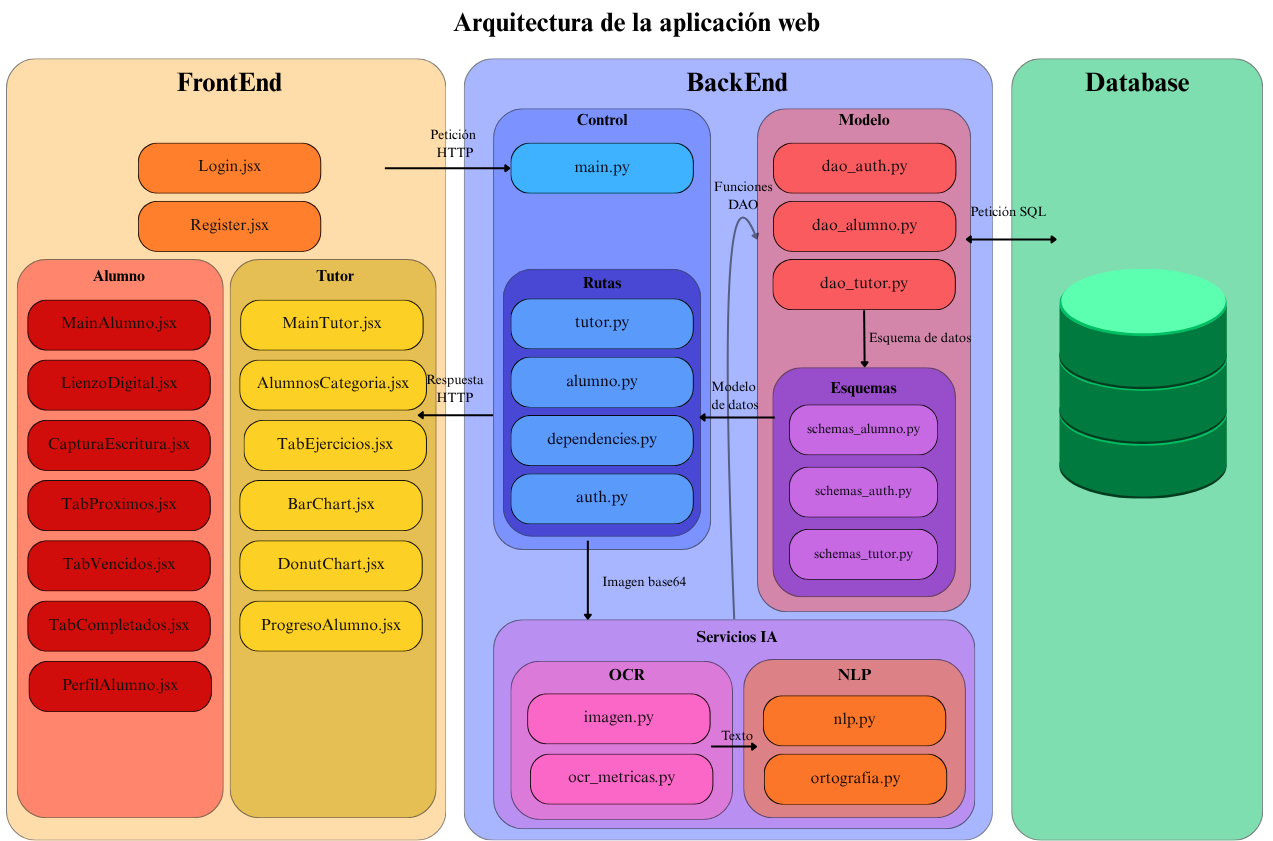
\includegraphics[width=0.95\linewidth]{Imagenes/Arquitectura.png}
        \caption{Diagrama de arquitectura del sistema}
        \label{fig:arquitectura_completa}
    \end{figure}
\end{landscape}

\subsection{Diseño de la base de datos}

El diseño de la base de datos define la capa de persistencia necesaria para soportar las operaciones de la plataforma, garantizando la integridad, seguridad y disponibilidad de la información. Siguiendo las formas normales para el modelado de bases de datos relacionalesw, el esquema ha sido normalizado hasta la Tercera Forma Normal (3NF), lo que permite mitigar anomalías de inserción, actualización y borrado, asegurando que la información de los usuarios y los resultados del análisis se almacenen de manera eficiente y sin redundancias innecesarias. 

En este apartado se detalla el modelo estructurado para gestionar la interacción entre los actores del sistema (tutores y alumnos), el almacenamiento del catálogo de ejercicios y la trazabilidad de la actividad académica. Asimismo, se describe la estrategia de almacenamiento empleada para registrar de forma eficiente las cargas útiles de imágenes y los resultados derivados del procesamiento asíncrono de los módulos de Inteligencia Artificial (OCR y NLP), fundamentando así la generación de recomendaciones personalizadas dentro de la arquitectura del sistema.

\subsubsection{Diagrama entidad-relación}
El diagrama entidad–relación constituye un elemento fundamental dentro del diseño de la aplicación web, ya que permite estructurar de manera formal la organización, almacenamiento y relación de los datos involucrados en el proceso de captura, procesamiento y evaluación de la escritura manuscrita.

La aplicación web propuesta gestiona el proceso de aprendizaje y evaluación de la escritura en alumnos de educación primaria. En este contexto, un tutor es responsable de supervisar a múltiples alumnos, asignándoles ejercicios orientados al desarrollo de habilidades de escritura.

El núcleo del sistema se encuentra en la entidad Intento, la cual representa cada ejecución de un ejercicio por parte del alumno. A partir de este intento, se procesa una imagen mediante OCR para obtener el texto digital, el cual es posteriormente analizado mediante NLP para evaluar la ortografía. De forma complementaria, se realiza un análisis caligráfico basado en características del trazo manuscrito.

Los resultados de estos análisis permiten generar recomendaciones personalizadas y actualizar el progreso del alumno, facilitando el seguimiento continuo de su desempeño.

En la Figura \ref{fig:er} se presenta el diagrama entidad–relación, el cual describe la estructura de datos y las relaciones entre las entidades involucradas en el proceso de evaluación de la escritura.

\begin{landscape}
\centering

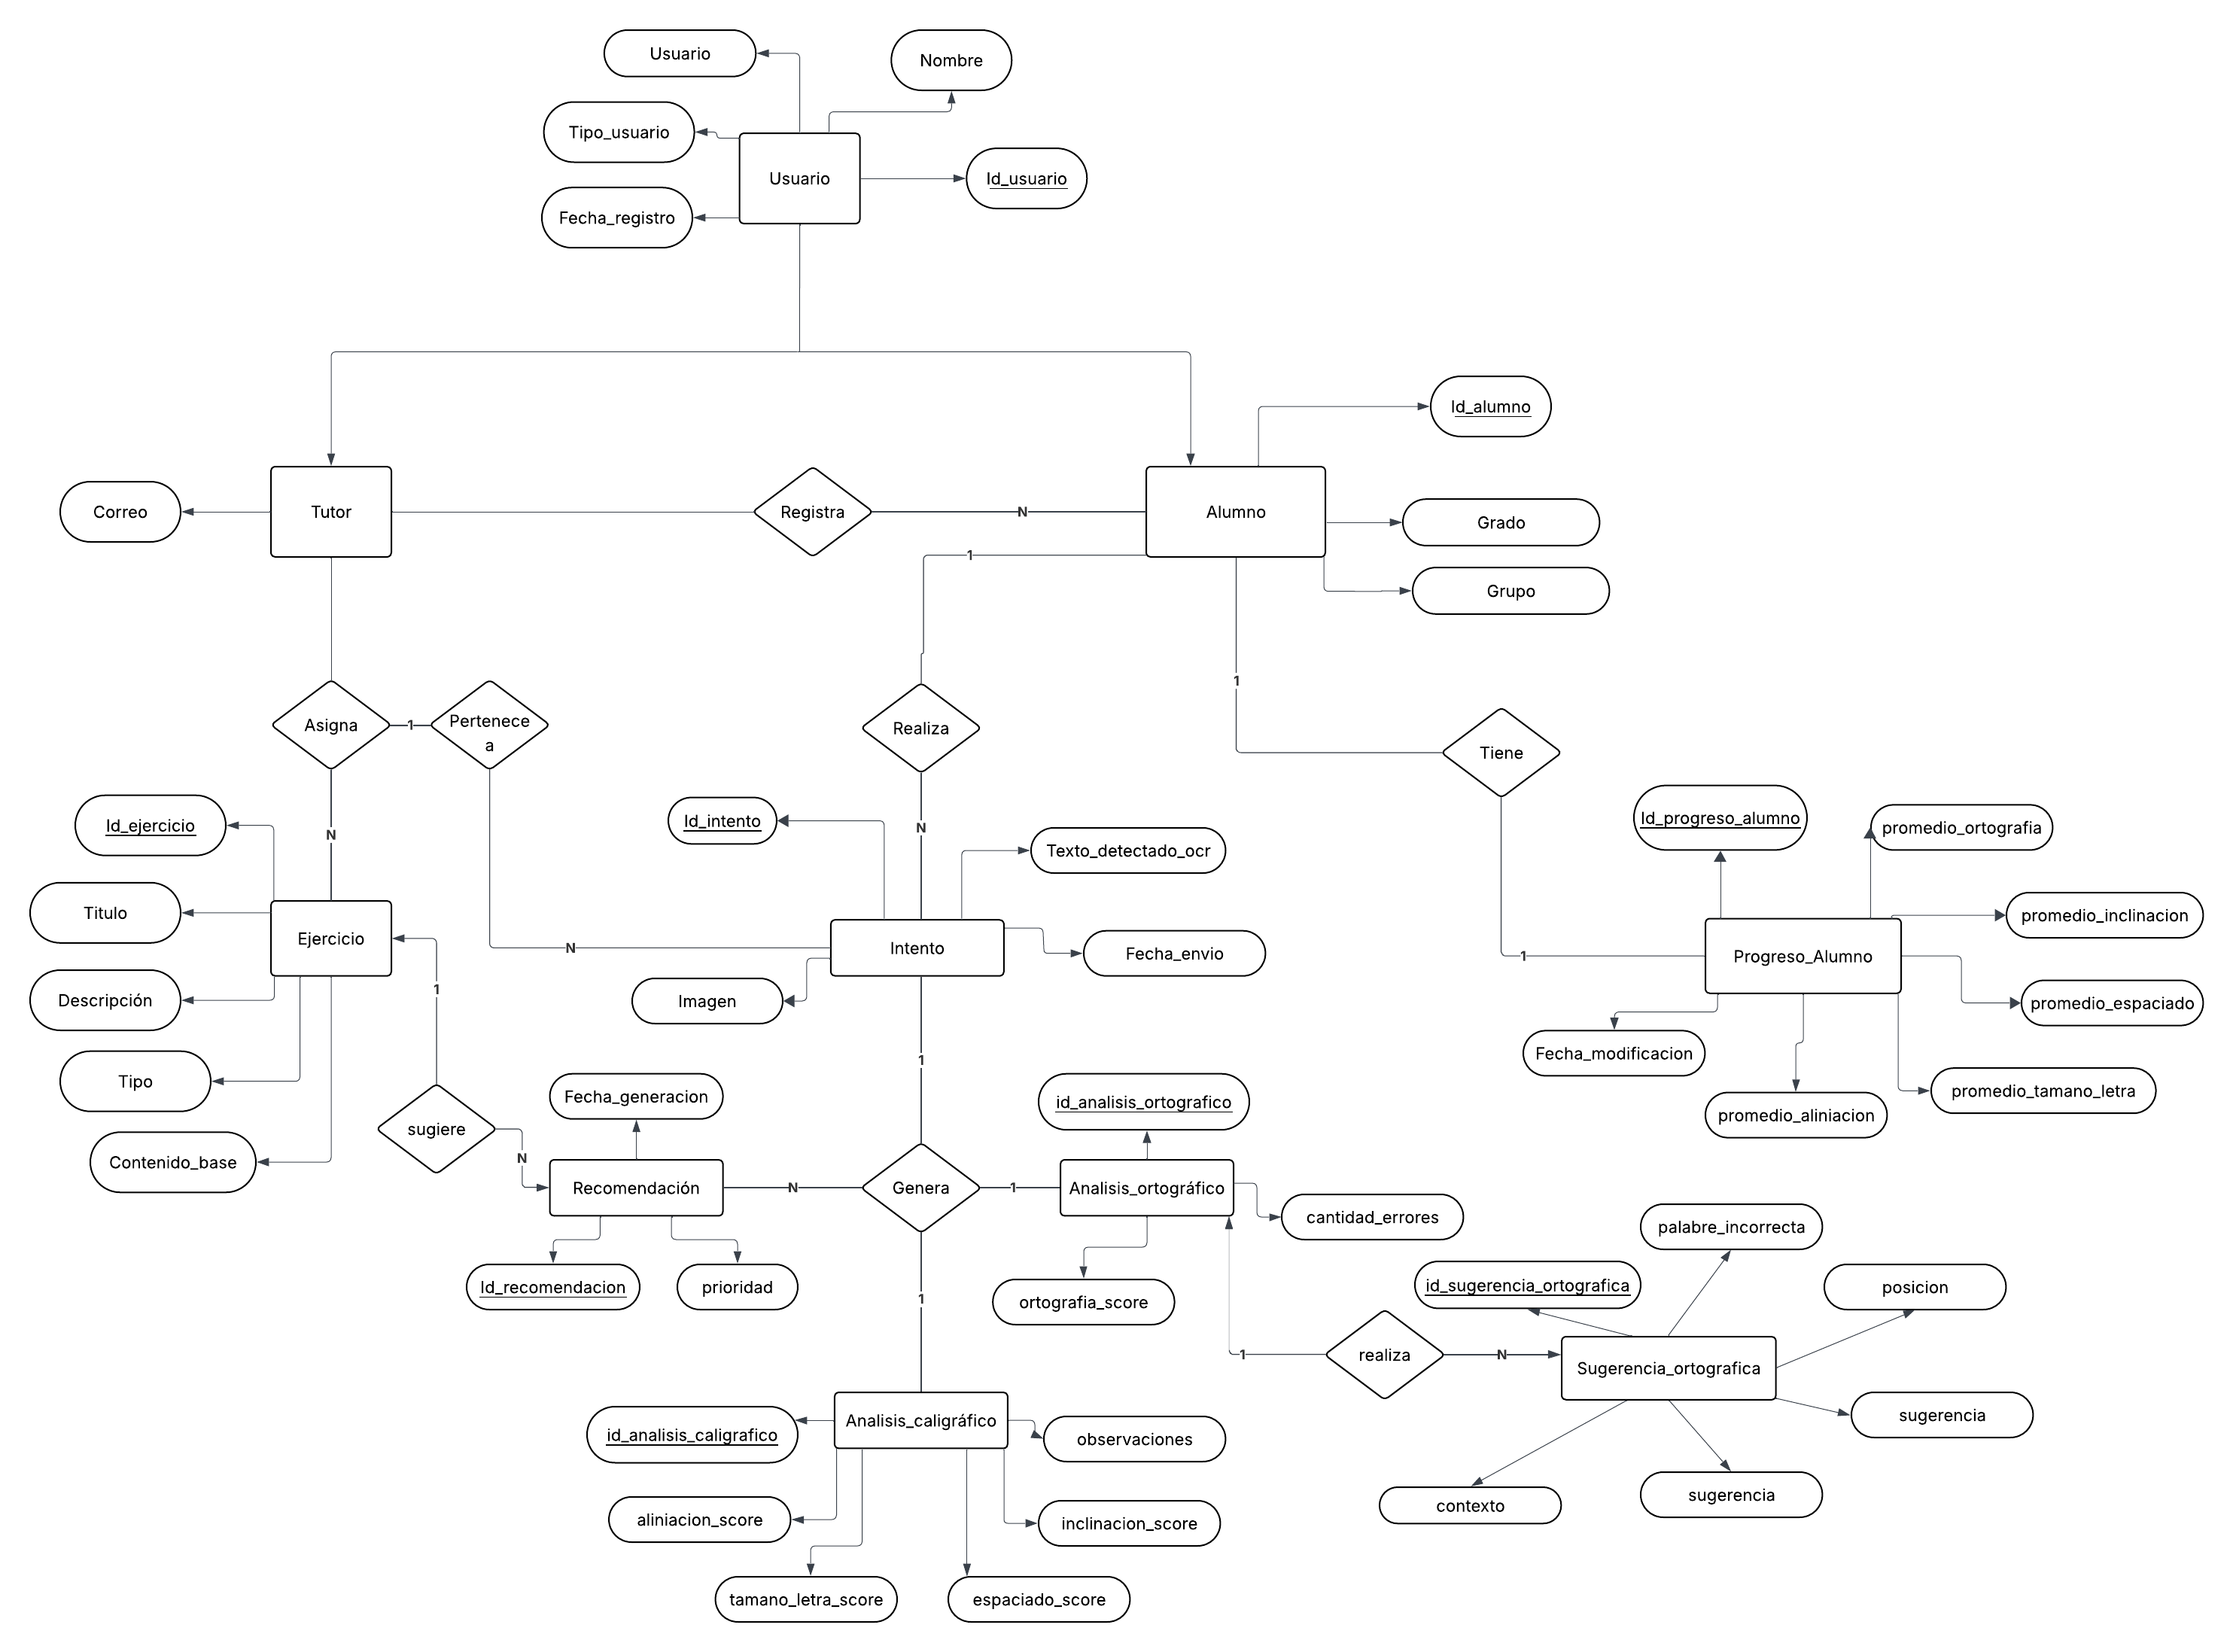
\includegraphics[
    width=0.95\linewidth,
    height=0.95\textheight,
    keepaspectratio
]{Imagenes/Diagrama-entidad-relacion.png}

\captionof{figure}{Diagrama entidad--relación propuesto}
\label{fig:er}

\end{landscape}

\subsubsection{Diccionario de entidades}

\textbf{A. Gestión de usuarios}

En la Tabla \ref{tab:entidades_usuarios} se describen las entidades correspondientes a la gestión de usuarios.

\begin{longtable}{|p{3.5cm}|p{7cm}|p{5cm}|}
\caption{Entidades de gestión de usuarios.}
\label{tab:entidades_usuarios} \\ \hline

\textbf{Entidad} & \textbf{Descripción} & \textbf{Atributos clave} \\ \hline
\endfirsthead

\hline
\textbf{Entidad} & \textbf{Descripción} & \textbf{Atributos clave} \\ \hline
\endhead

Estatus & Entidad que permite indicar el estado de un registro, facilitando su control sin eliminación física. &
id\_estatus, descripcion \\ \hline

Usuario & Entidad base para el acceso a la aplicación web. &
id\_usuario, nombre, tipo\_usuario, fecha\_registro, FK id\_estatus \\ \hline

Tutor & Usuario con permisos para registrar alumnos y asignar ejercicios. &
correo \\ \hline

Alumno & Usuario final que realiza los ejercicios de escritura. &
id\_alumno, grado, grupo \\ \hline

\end{longtable}

Las entidades presentadas permiten gestionar el acceso y la organización de los usuarios dentro del sistema.

\textbf{B. Proceso de evaluación}

En la Tabla \ref{tab:entidades_evaluacion} se presentan las entidades relacionadas con el proceso de evaluación de la escritura.

\begin{longtable}{|p{3.5cm}|p{7cm}|p{5cm}|}
\caption{Entidades del proceso de evaluación del sistema}
\label{tab:entidades_evaluacion} \\ \hline

\textbf{Entidad} & \textbf{Descripción} & \textbf{Atributos clave} \\ \hline
\endfirsthead

\hline
\textbf{Entidad} & \textbf{Descripción} & \textbf{Atributos clave} \\ \hline
\endhead

Ejercicio & Catalogo de ejercicios. &
id\_ejercicio, titulo, contenido\_base, tipo \\ \hline

Ejercicio\_Tutor & Ejercicios asignados por el tutor. & id\_ejercicio\_tutor, FK id\_tutor, FK id\_ejercicio, fecha\_inicio y fecha\_fin, FK id\_estatus\\ \hline

Intento & Ejecución de un ejercicio por parte del alumno. &
id\_intento, FK id\_alumno, FK id\_ejercicio\_tutor, imagen, texto\_detectado\_ocr, fecha\_envio \\ \hline

Analisis\_ortografico & Resultado del procesamiento NLP. &
id\_analisis\_ortografico, cantidad\_errores, ortografia\_score \\ \hline

sugerencia\_ortogra-
fica & Errores detetctados del procesamiento NLP, en conjunto con su sugerencia. &
id\_sugerencia\_ortografica, palabra\_incorrecta, posicion, sugerencia, contexto \\ \hline

Analisis\_caligrafico & Resultado del análisis del trazo manuscrito. &
id\_analisis\_caligrafico, inclinacion\_score, espaciado\_score, tamano\_letra\_score \\ \hline

\end{longtable}

Estas entidades representan el núcleo del procesamiento de la información dentro de la aplicación web.

\textbf{C. Seguimiento y retroalimentación}

En la Tabla \ref{tab:entidades_SR} se describen las entidades asociadas al seguimiento y retroalimentación del alumno.

\begin{longtable}{|p{3.5cm}|p{7cm}|p{5cm}|}
\caption{Entidades del proceso de evaluación del sistema}
\label{tab:entidades_SR} \\ \hline

\textbf{Entidad} & \textbf{Descripción} & \textbf{Atributos clave} \\ \hline
\endfirsthead

\hline
\textbf{Entidad} & \textbf{Descripción} & \textbf{Atributos clave} \\ \hline
\endhead

Recomendación & Sugerencia generada automáticamente. &
id\_recomendacion, FK Id\_intento, FK id\_ejercicio, fecha\_generación, estado, prioridad. \\ \hline

Progreso\_alumno & Indicadores acumulados del desempeño. &
id\_progreso\_alumno,FK id\_alumno,promedio\_orto-
grafia, promedio\_caligrafia \\ \hline

\end{longtable}

Estas entidades permiten el seguimiento del desempeño y la generación de retroalimentación personalizada.



\subsubsection{Análisis de relaciones}

El modelo entidad--relación define las interacciones entre las entidades del sistema mediante relaciones con cardinalidades específicas, las cuales permiten representar la forma en que los datos se asocian dentro del proceso de evaluación de la escritura.

A continuación, se describen las principales relaciones identificadas en el modelo:

\begin{itemize}
    \item \textbf{Herencia (Usuario $\rightarrow$ Tutor / Alumno)}
\end{itemize}

Se establece una relación de especialización en la cual la entidad Usuario actúa como entidad base, de la que derivan los roles de Tutor y Alumno. Esta estructura permite reutilizar atributos comunes, como nombre y fecha de registro, y asignar funcionalidades específicas según el tipo de usuario.

\begin{itemize}
    \item \textbf{Tutor -- Alumno (1:N)}
\end{itemize}

Un tutor puede supervisar a muchos alumnos, mientras que cada alumno está asociado a un único tutor responsable.

\begin{itemize}
    \item \textbf{Tutor -- Ejercicio (M:N)}
\end{itemize}

Un tutor puede asignar múltiples ejercicios del catálogo, y un mismo 
ejercicio del catálogo puede ser asignado por múltiples tutores. Esta 
relación se en la entidad de asociación \textit{Ejercicio\_Tutor}.

\begin{itemize}
    \item \textbf{Alumno -- Intento (1:N)}
\end{itemize}

Un alumno puede realizar múltiples intentos a lo largo del tiempo, ya que cada intento representa una ejecución individual de un ejercicio. Esta relación permite almacenar el historial de participación del alumno.

\begin{itemize}
    \item \textbf{Intento -- Análisis ortográfico (1:1)}
\end{itemize}

Cada intento genera exactamente un análisis ortográfico, el cual contiene la evaluación del texto detectado mediante NLP, incluyendo errores y sugerencias.

\begin{itemize}
    \item \textbf{Intento -- Análisis caligráfico (1:1)}
\end{itemize}

Cada intento genera un único análisis caligráfico, el cual evalúa características del trazo manuscrito como alineación, tamaño y espaciado.

\begin{itemize}
    \item \textbf{Intento -- Recomendación (1:N)}
\end{itemize}

Un intento puede generar múltiples recomendaciones, dependiendo de la cantidad y tipo de errores detectados en los análisis realizados.

\begin{itemize}
    \item \textbf{Alumno -- Progreso\_alumno (1:1)}
\end{itemize}

Cada alumno cuenta con un único registro en la entidad Progreso\_alumno, el cual almacena indicadores acumulados de su desempeño, como promedios de ortografía y caligrafía.

Esta relación nos permite obtener un promedio global para el análisis ortográfico y caligráfico, facilitando la calsificación de los alumnos.

\subsubsection{Diagrama relacional}

En la Figura \ref{fig:rel} se presenta el diagrama relacional de la aplicación web, donde se definen las tablas, sus atributos, así como las relaciones mediante llaves primarias y foráneas.

\begin{landscape}
    
\begin{figure}[H]
    \centering
    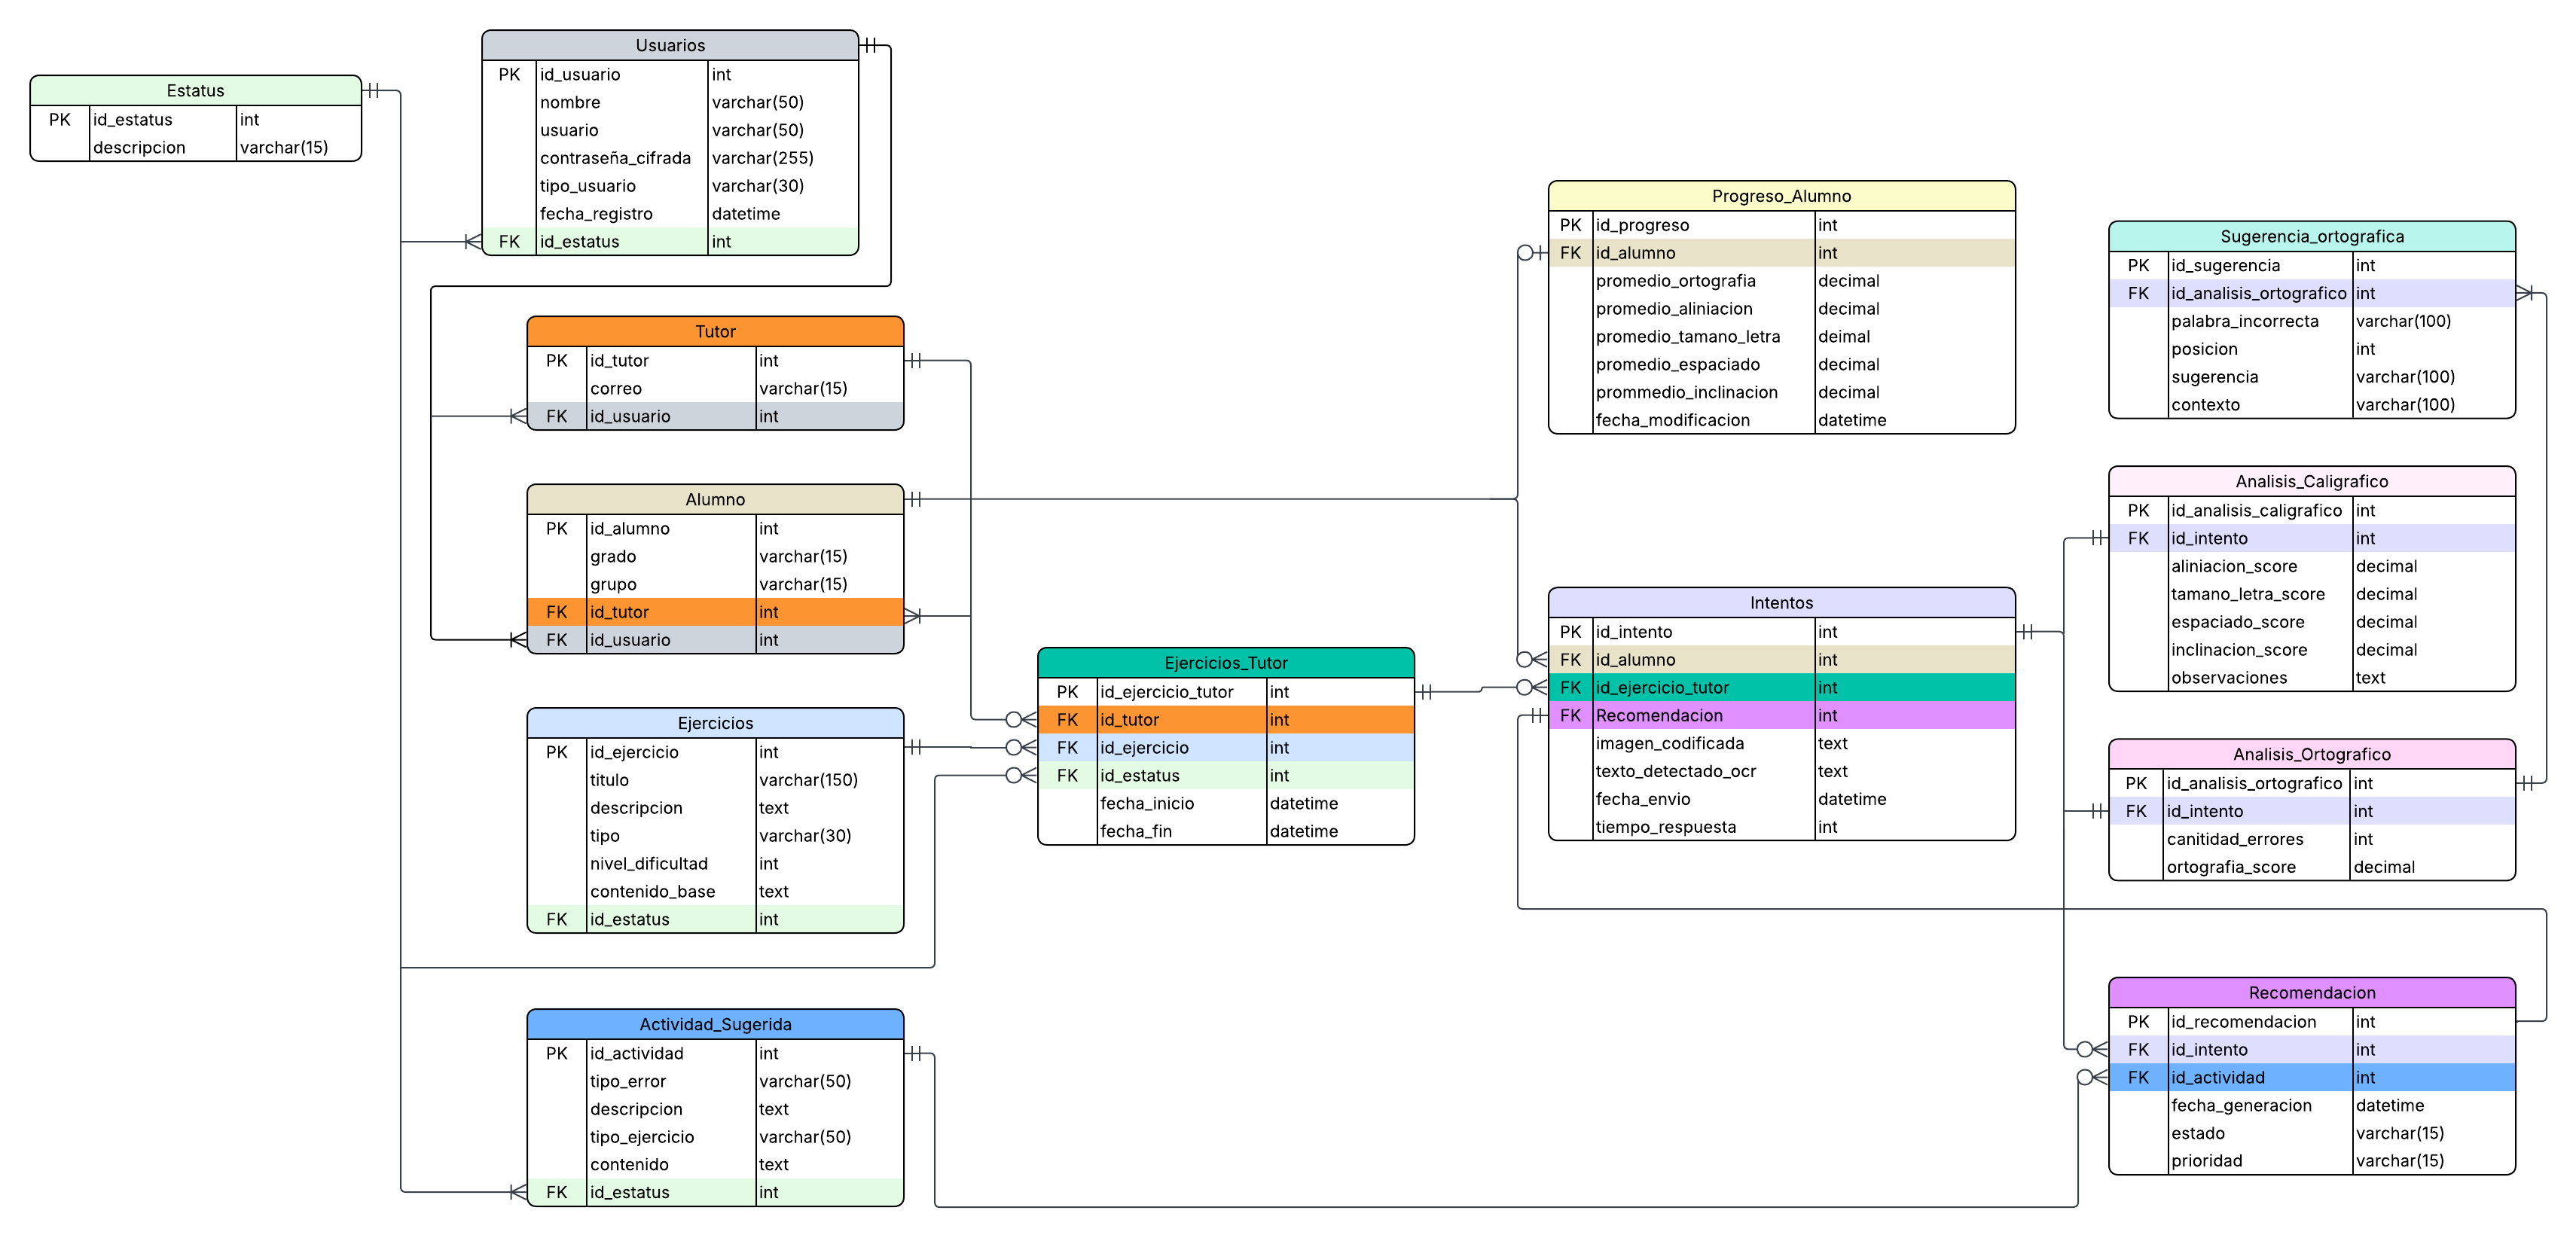
\includegraphics[
        width=\linewidth,
        keepaspectratio
    ]{Imagenes/DiagramaRelaiconal-2.png}

    \caption{Diagrama relacional propuesto}
    \label{fig:rel}
\end{figure}

\end{landscape}

\subsubsection{Decisiones de diseño de base de datos}

\paragraph{Gestión del texto detectado (OCR)}

El atributo texto\_detectado\_ocr en la entidad Intento representa un elemento crítico dentro de la aplicación web, ya que corresponde a la salida generada por el módulo de reconocimiento óptico de caracteres (OCR). Este dato constituye la entrada principal para el procesamiento mediante técnicas de procesamiento de lenguaje natural (NLP), por lo que su correcta generación y almacenamiento es fundamental para garantizar la calidad del análisis ortográfico.

El uso de este formato proporciona flexibilidad y evita la rigidez de un esquema relacional estrictamente normalizado, facilitando futuras ampliaciones del sistema.

\paragraph{Cálculo del progreso del alumno}

La entidad \textit{Progreso\_alumno} funciona como una tabla de agregación que almacena indicadores globales del desempeño del estudiante. Su actualización se realiza mediante triggers a nivel de base de datos, los cuales recalculan automáticamente los promedios de ortografía y caligrafía al registrar un nuevo inteno.

Este enfoque se justifica por las siguientes razones:

\begin{itemize}
    \item \textbf{Atomicidad:} el trigger se ejecuta dentro de la misma transacción que el INSERT del intento, garantizando que \textit{Progreso\_alumno} siempre refleje el estado actualizado sin depender de una llamada adicional desde el controlador.

    \item \textbf{Consistencia:} se elimina el riesgo de inconsistencia de datos ante un fallo del backend posterior a la inserción del intento pero previo a la actualización del progreso.

    \item \textbf{Separación de responsabilidades:} el controlador no requiere conocer la lógica de cálculo de promedios, delegando esa responsabilidad a la base de datos, lo cual es coherente con el patrón de diseño MVC adoptado en el sistema.

\end{itemize}

\paragraph{Gestión del historial y trazabilidad}

La vista \textit{vw\_historial\_alumno} permite mantener un registro cronológico de los resultados obtenidos por el alumno en cada intento, sin comprometer la normalización del modelo de datos. A diferencia de una tabla adicional, la vista consolida la información existente en las entidades Intento, Analisis\_ortografico y Analisis\_caligrafico mediante una consulta predefinida, evitando la redundancia de datos. 

\subsection{Diagrama de clases del sistema}

Con el objetivo de definir la estructura estática del sistema, se presenta el diagrama de clases, el cual describe las principales entidades, sus atributos y las relaciones existentes entre ellas.

\begin{figure}[H]
    \centering
    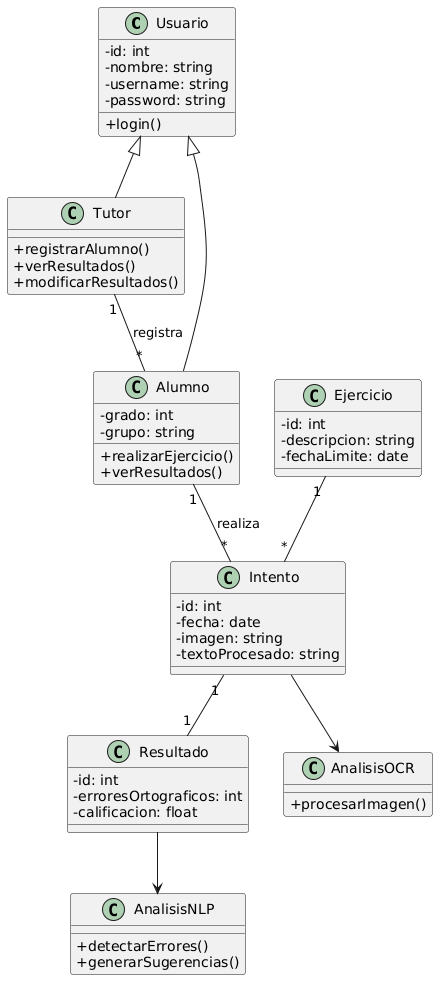
\includegraphics[width=0.60\textwidth]{Imagenes/DiagramaDeClases.png}
    \caption{Diagrama de clases del sistema}
    \label{fig:diagrama_clases}
\end{figure}

El diagrama de clases representa la estructura estática del sistema, mostrando las principales entidades, sus atributos y las relaciones entre ellas. Se observa una jerarquía de herencia donde la clase \textit{Usuario} es la base para los actores \textit{Tutor} y \textit{Alumno}. Asimismo, se modelan los elementos centrales del sistema como \textit{Ejercicio}, \textit{Intento} y \textit{Resultado}, los cuales permiten gestionar el proceso de captura, análisis y retroalimentación de la escritura. Finalmente, se integran los módulos de procesamiento \textit{AnalisisOCR} y \textit{AnalisisNLP}, responsables de la conversión de imágenes a texto y la detección de errores ortográficos respectivamente.

%------------------------------------------------

\subsection{Diagrama de secuencia del procesamiento de ejercicios}

Con el propósito de representar el comportamiento dinámico del sistema, se presenta el diagrama de secuencia correspondiente al proceso de análisis de ejercicios, el cual describe la interacción entre los diferentes componentes involucrados desde la captura de la imagen hasta la generación de resultados.

\begin{figure}[H]
    \centering
    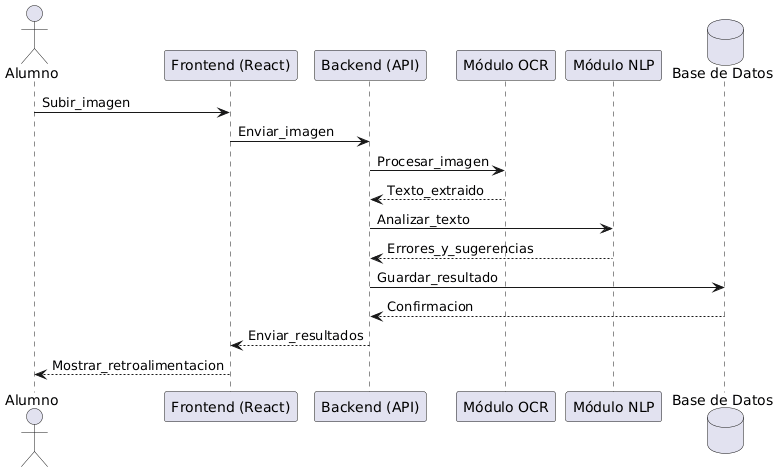
\includegraphics[width=0.75\textwidth]{Imagenes/DiagramaDeSecuencia.png}
    \caption{Diagrama de secuencia del procesamiento de ejercicios}
    \label{fig:diagrama_secuencia}
\end{figure}

El diagrama muestra cómo el alumno interactúa con la interfaz para enviar una imagen, la cual es procesada por el backend mediante un módulo OCR para la extracción de texto. Posteriormente, el texto es analizado por el módulo NLP para identificar errores ortográficos y generar sugerencias. Finalmente, los resultados son almacenados en la base de datos y enviados al usuario para su visualización.

%------------------------------------------------

\subsection{Diagrama de actividad del procesamiento de ejercicios}

Con el propósito de representar el flujo de actividades del sistema, se presenta el diagrama de actividad correspondiente al proceso de análisis de ejercicios, el cual describe de manera secuencial las acciones realizadas desde la interacción del usuario hasta la generación de resultados.

\begin{figure}[H]
    \centering
    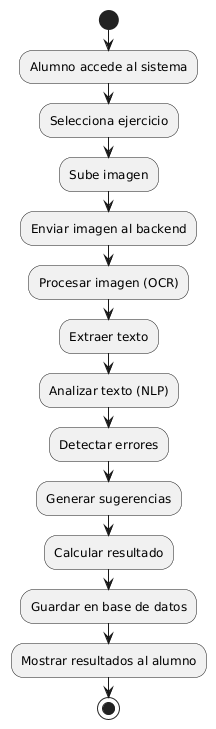
\includegraphics[width=0.35\textwidth]{Imagenes/DiagramaDeActividad.png}
    \caption{Diagrama de actividad del procesamiento de ejercicios}
    \label{fig:diagrama_actividad}
\end{figure}

El diagrama muestra la secuencia de actividades que se llevan a cabo cuando un alumno realiza un ejercicio, comenzando desde la selección y envío de la imagen, pasando por el procesamiento mediante OCR y el análisis con técnicas de procesamiento de lenguaje natural, hasta la generación y almacenamiento de los resultados, los cuales son finalmente presentados al usuario.

%------------------------------------------------

%\subsection{Diagrama de estados del proceso de evaluación}

%Con el propósito de representar los diferentes estados por los que pasa un ejercicio dentro del sistema, se presenta el diagrama de estados, el cual describe el ciclo de vida del proceso de evaluación desde su inicio hasta la presentación de resultados.

%\begin{figure}[H]
%    \centering
%    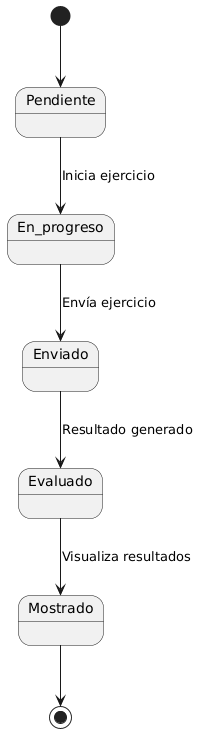
\includegraphics[width=0.60\textwidth]{Imagenes/DiagramaDeEstado.png}
%    \caption{Diagrama de estados del proceso de evaluación}
%    \label{fig:diagrama_estados}
%\end{figure}

%El diagrama muestra los estados principales por los que transita un ejercicio dentro del sistema, desde que se encuentra pendiente, pasando por su desarrollo y envío, hasta su evaluación y visualización por parte del usuario. Este modelo permite comprender el comportamiento general del sistema durante el proceso de evaluación sin detallar los procesos internos.
            
%------------------------------------------------

\subsection{Diagrama de componentes del sistema}

Con el objetivo de representar la estructura modular del sistema, se presenta el diagrama de componentes, el cual muestra la organización de los principales elementos de software y sus interacciones dentro de la arquitectura de la aplicación.

\begin{figure}[H]
    \centering
    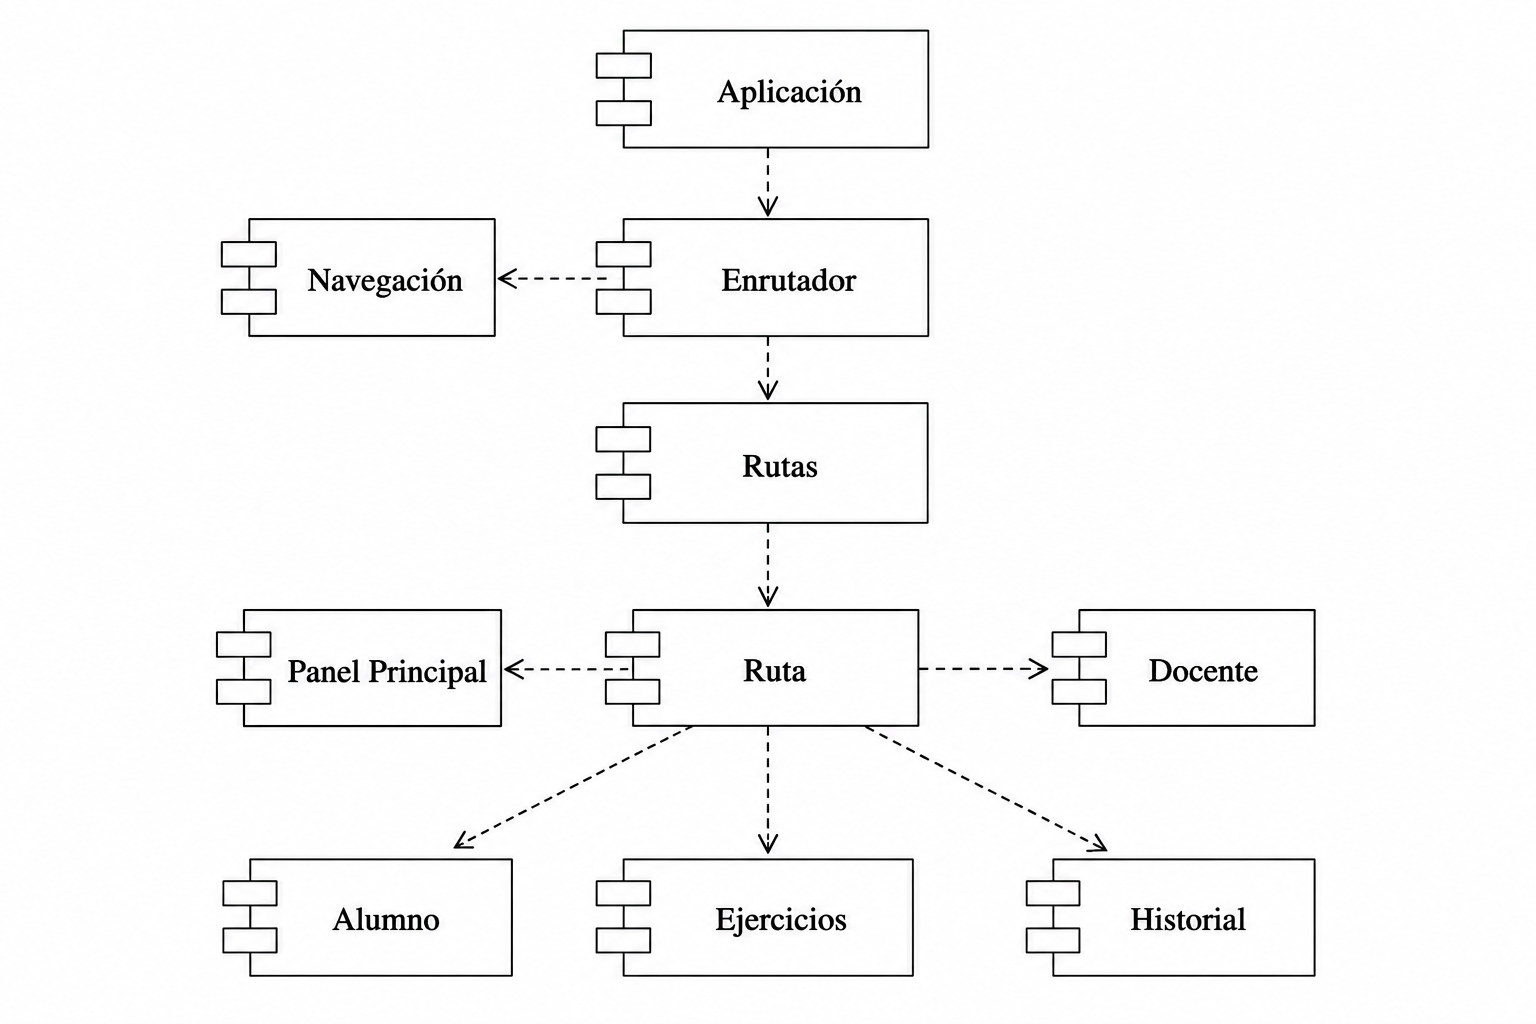
\includegraphics[width=0.65\textwidth]{Imagenes/DiagramaDeComponentess.png}
    \caption{Diagrama de componentes del sistema}
    \label{fig:diagrama_componentes}
\end{figure}

El diagrama muestra la separación del sistema en tres capas principales: cliente, servidor y persistencia. El frontend se encarga de la interacción con el usuario, mientras que el backend gestiona la lógica del sistema y coordina el procesamiento mediante los módulos OCR y NLP. Finalmente, la base de datos permite almacenar la información generada y consultada durante la operación del sistema.

La separación de los módulos de procesamiento OCR y NLP permite una arquitectura más flexible y escalable, ya que cada componente puede ser optimizado o actualizado de manera independiente. Además, esta división facilita el mantenimiento del sistema y mejora la eficiencia en el procesamiento de la información.

%------------------------------------------------

\subsection{Diagrama de despliegue del sistema}

Con el objetivo de representar la distribución física del sistema, se presenta el diagrama de despliegue, el cual muestra los nodos de hardware involucrados y la forma en que los componentes de software se encuentran distribuidos dentro de la arquitectura de la aplicación.

\begin{figure}[H]
    \centering
    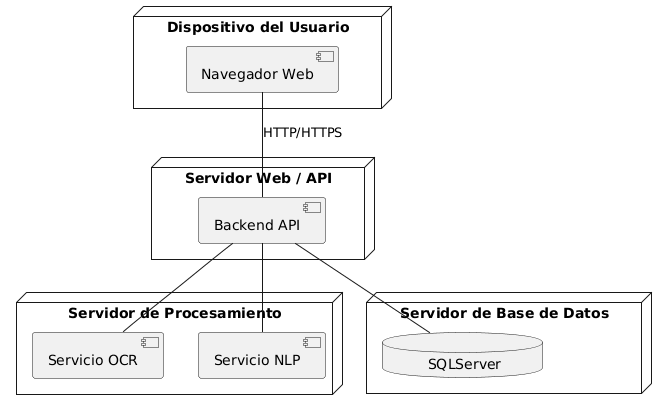
\includegraphics[width=0.65\textwidth]{Imagenes/DiagramaDeDespliegue.png}
    \caption{Diagrama de despliegue del sistema}
    \label{fig:diagrama_despliegue}
\end{figure}

El diagrama muestra la organización del sistema en distintos nodos físicos, incluyendo el dispositivo del usuario, el servidor de aplicaciones, el servidor de procesamiento y el servidor de base de datos. En el dispositivo del usuario se ejecuta el navegador web, desde donde se realizan las solicitudes al backend mediante protocolos HTTP/HTTPS. El servidor de aplicaciones gestiona la lógica del sistema, mientras que los servicios de procesamiento OCR y NLP se encargan de analizar la información recibida. Finalmente, el servidor de base de datos permite almacenar y consultar la información generada durante la operación del sistema.

Asimismo, se observa la separación de los servicios en distintos nodos, lo cual permite una mejor distribución de la carga y facilita la escalabilidad del sistema.
%% ─────────────────────────────────────────────────────────────────────────────
%  Sección 4.X  Arquitectura del Módulo de Gestión de Ejercicios
%  Insertar en el Capítulo 4: Diseño, después del módulo de Autenticación
%  y antes del módulo OCR/NLP.
% ─────────────────────────────────────────────────────────────────────────────

\subsection{Arquitectura del Módulo de Gestión de Ejercicios}

El módulo de gestión de ejercicios administra el ciclo de vida completo
de las actividades de escritura dentro de la plataforma. Su diseño contempla
dos actores con responsabilidades distintas: el tutor, que selecciona
ejercicios del catálogo y los asigna a sus alumnos con una vigencia
determinada; y el alumno, que consulta los ejercicios disponibles
clasificados por su estado. El módulo también incorpora un proceso
automatizado que cierra los ejercicios cuya fecha de vencimiento ha
sido alcanzada, garantizando la coherencia del estado del sistema sin
intervención manual.

La arquitectura del módulo se divide en tres componentes principales:

\begin{enumerate}
    \item \textbf{Capa de Presentación (Front-End):} Compuesta por los
    componentes \texttt{TabEjercicios.jsx} (vista del tutor para gestionar
    asignaciones), \texttt{TabProximos.jsx}, \texttt{TabCompletados.jsx}
    y \texttt{TabVencidos.jsx} (vistas del alumno que clasifican los
    ejercicios según su estado). Cada componente consulta su endpoint
    correspondiente y renderiza la información sin lógica de negocio
    propia.

    \item \textbf{Capa de Lógica de Negocio (Back-End):} Implementada
    en el controlador \texttt{ejercicios.py} mediante FastAPI. Gestiona
    la consulta del catálogo, la activación y desactivación de ejercicios
    por parte del tutor, y la consulta de ejercicios en sus tres estados
    posibles desde la perspectiva del alumno. Adicionalmente, el proceso
    \texttt{cerrar\_ejercicio.py} implementa un scheduler que verifica
    y cierra automáticamente los ejercicios vencidos cada hora.

    \item \textbf{Capa de Persistencia (Base de Datos):} El módulo opera
    sobre dos tablas principales: \texttt{Ejercicios}, que actúa como
    catálogo inmutable de actividades disponibles en la plataforma, y
    \texttt{Ejercicios\_Tutor}, que representa la asignación de un
    ejercicio del catálogo a un tutor específico, con su propio ciclo de
    vida controlado por el campo \texttt{id\_estatus} y la fecha
    \texttt{fecha\_desactivacion}.
\end{enumerate}

% ─────────────────────────────────────────────────────────
\subsubsection{Diseño del Ciclo de Vida de un Ejercicio}

Un ejercicio atraviesa los siguientes estados a lo largo de su ciclo de
vida dentro del sistema:

\begin{enumerate}
    \item \textbf{Disponible en catálogo:} el ejercicio existe en la tabla
    \texttt{Ejercicios} con \texttt{id\_estatus = 1} y puede ser
    seleccionado por cualquier tutor para su asignación.

    \item \textbf{Activo:} el tutor ha creado un registro en
    \texttt{Ejercicios\_Tutor} con \texttt{id\_estatus = 1}. A partir de
    este momento, el ejercicio es visible para los alumnos del tutor en
    su panel de ejercicios próximos.

    \item \textbf{Vencido:} el ejercicio transiciona a
    \texttt{id\_estatus = 2} por uno de dos mecanismos: desactivación
    manual por parte del tutor mediante el endpoint de eliminación, o
    cierre automático por el scheduler cuando la fecha
    \texttt{fecha\_desactivacion} es anterior a la fecha y hora actuales
    del servidor. Un ejercicio vencido deja de aparecer en la lista de
    próximos del alumno y pasa a la lista de vencidos si no fue entregado,
    o permanece en completados si el alumno ya realizó un intento.
\end{enumerate}

\noindent \textit{Nota de diseño}: el sistema no elimina físicamente los
registros de \texttt{Ejercicios\_Tutor}. La transición entre estados se
gestiona exclusivamente mediante el campo \texttt{id\_estatus}, lo que
preserva la trazabilidad histórica de las asignaciones y permite al tutor
consultar ejercicios previamente activos sin pérdida de información.

% ─────────────────────────────────────────────────────────
\subsubsection{Diseño del Flujo de Interacción}

El módulo contempla tres flujos principales de interacción.

\textbf{Flujo de Asignación de Ejercicio (Tutor):}
\begin{enumerate}
    \item El tutor accede a su panel y solicita el catálogo de ejercicios
    disponibles mediante una petición \texttt{GET} al endpoint público
    \texttt{/api/ejercicios/}.
    \item El tutor selecciona un ejercicio y establece opcionalmente una
    fecha de vencimiento. El Front-End envía una petición \texttt{POST}
    al endpoint \texttt{/api/ejercicios/tutor} con el identificador del
    ejercicio y la fecha de cierre.
    \item El Back-End verifica mediante JWT que el \texttt{id\_usuario}
    del token coincide con el \texttt{id\_usuario} del payload, evitando
    que un tutor active ejercicios en nombre de otro.
    \item Se verifica que el tutor no tenga ya activo el mismo ejercicio.
    En caso de duplicado, se retorna \texttt{400 Bad Request}.
    \item Se inserta un nuevo registro en \texttt{Ejercicios\_Tutor} con
    \texttt{id\_estatus = 1}. El ejercicio queda inmediatamente disponible
    para los alumnos del tutor.
\end{enumerate}

\textbf{Flujo de Consulta de Ejercicios (Alumno):}

Desde la perspectiva del alumno, los ejercicios se presentan clasificados
en tres pestañas. La lógica de clasificación reside íntegramente en el
Back-End mediante tres consultas SQL independientes:

\begin{itemize}
    \item \textbf{Próximos:} ejercicios activos (\texttt{id\_estatus = 1})
    asignados por el tutor del alumno que aún no tienen un intento
    registrado por ese alumno. Se excluyen mediante una subconsulta
    \texttt{NOT IN} sobre la tabla \texttt{Intentos}.

    \item \textbf{Completados:} ejercicios que tienen al menos un intento
    registrado por el alumno. Se retorna únicamente el intento más reciente
    por ejercicio, determinado mediante la función de ventana
    \texttt{ROW\_NUMBER() OVER (PARTITION BY id\_ejercicio\_tutor ORDER BY
    fecha\_envio DESC)}, incluyendo la calificación y retroalimentación
    del tutor si ya fueron registradas.

    \item \textbf{Vencidos:} ejercicios con \texttt{id\_estatus = 2} que
    no tienen ningún intento registrado por el alumno, es decir, los que
    el alumno no alcanzó a entregar antes del cierre.
\end{itemize}

\paragraph{Flujo de Cierre Automático (Scheduler):}
\begin{enumerate}
    \item Al iniciar el servidor, el evento \texttt{startup} de FastAPI
    invoca \texttt{iniciar\_scheduler()}, que registra una tarea periódica
    con una frecuencia de ejecución de una hora mediante la biblioteca
    APScheduler.
    \item Cada hora, la tarea \texttt{cerrar\_ejercicios\_vencidos()}
    ejecuta un \texttt{UPDATE} sobre la tabla \texttt{Ejercicios\_Tutor},
    transitando a \texttt{id\_estatus = 2} todos los registros cuya
    \texttt{fecha\_desactivacion} sea distinta de nulo y anterior a la
    fecha y hora actuales del servidor (\texttt{GETDATE()}).
    \item La operación es idempotente: ejecutarla múltiples veces sobre
    los mismos datos no produce efectos secundarios, ya que la condición
    \texttt{id\_estatus = 1} del filtro impide modificar registros ya
    cerrados.
\end{enumerate}

% ─────────────────────────────────────────────────────────
\subsubsection{Diseño de APIs}

Para soportar los flujos descritos, el diseño de la API contempla los
siguientes endpoints en el controlador \texttt{ejercicios.py}:

\textbf{Endpoint 1:} Consulta del Catálogo

El endpoint \texttt{/api/ejercicios/} opera mediante el método \texttt{GET}
y no requiere autenticación. Retorna todos los ejercicios con
\texttt{id\_estatus = 1} disponibles en la tabla \texttt{Ejercicios}.

\textbf{Endpoint 2:} Consulta de Ejercicios Activos del Tutor

El endpoint \texttt{/api/ejercicios/tutor/\{id\_usuario\}} opera mediante
el método \texttt{GET} y requiere autenticación JWT con rol de tutor.
Retorna los ejercicios que el tutor ha activado y que se encuentran
actualmente con \texttt{id\_estatus = 1}.

\textbf{Endpoint 3:} Activación de Ejercicio

El endpoint \texttt{/api/ejercicios/tutor} opera mediante el método
\texttt{POST} y requiere autenticación JWT con rol de tutor. Recibe el
identificador del ejercicio del catálogo y una fecha de vencimiento
opcional.

\begin{lstlisting}[language=json, caption={Payload de solicitud del endpoint de activación de ejercicio}, label={lst:ejercicio-create}]
/* Solicitud */
{
  "id_ejercicio": <integer>,
  "id_usuario":   <integer>,
  "fecha_fin":    "datetime | null"
}

/* Respuesta 201 Created */
{
  "message": "Ejercicio activado correctamente"
}
\end{lstlisting}

\textbf{Endpoint 4:} Desactivación Manual de Ejercicio

El endpoint \texttt{/api/ejercicios/tutor/\{id\_usuario\}/\{id\_ejercicio\}}
opera mediante el método \texttt{DELETE} y requiere autenticación JWT con
rol de tutor. Actualiza el campo \texttt{id\_estatus} a 2 en el registro
correspondiente de \texttt{Ejercicios\_Tutor}, sin eliminar el registro
físicamente.

\textbf{Endpoints 5, 6 y 7:} Consulta de Ejercicios del Alumno

Los endpoints \texttt{/api/ejercicios/alumno/\{id\_alumno\}/proximos},
\texttt{/api/ejercicios/alumno/\{id\_alumno\}/completados} y
\texttt{/api/ejercicios/alumno/\{id\_alumno\}/vencidos} operan mediante
el método \texttt{GET} y requieren autenticación JWT con rol de alumno.
En los tres casos, el Back-End verifica que el \texttt{id\_alumno} de la
ruta coincida con el \texttt{id\_usuario} del token, retornando
\texttt{403 Forbidden} en caso de discrepancia.

La Tabla~\ref{tab:endpoints-ejercicios} resume los endpoints del módulo
con su método y nivel de acceso correspondiente.

\begin{table}[H]
\centering
\caption{Endpoints del módulo de gestión de ejercicios}
\label{tab:endpoints-ejercicios}
\begin{tabular}{|l|l|l|}
\hline
\textbf{Endpoint} & \textbf{Método} & \textbf{Acceso requerido} \\
\hline
\texttt{/api/ejercicios/}
    & GET    & Público \\
\texttt{/api/ejercicios/tutor/\{id\_usuario\}}
    & GET    & Tutor (JWT) \\
\texttt{/api/ejercicios/tutor}
    & POST   & Tutor (JWT) \\
\texttt{/api/ejercicios/tutor/\{id\_usuario\}/\{id\_ejercicio\}}
    & DELETE & Tutor (JWT) \\
\texttt{/api/ejercicios/alumno/\{id\_alumno\}/proximos}
    & GET    & Alumno (JWT) \\
\texttt{/api/ejercicios/alumno/\{id\_alumno\}/completados}
    & GET    & Alumno (JWT) \\
\texttt{/api/ejercicios/alumno/\{id\_alumno\}/vencidos}
    & GET    & Alumno (JWT) \\
\hline
\end{tabular}
\end{table}

\subsection{Arquitectura del Módulo de Progreso y Recomendaciones}

El módulo de progreso y recomendaciones centraliza el seguimiento
longitudinal del desempeño del alumno y expone al tutor las herramientas
de supervisión grupal necesarias para tomar decisiones pedagógicas
informadas. A diferencia de los módulos anteriores, cuyo alcance es
transaccional —un intento, un ejercicio, una autenticación—, este módulo
opera sobre el historial acumulado del alumno, sintetizando múltiples
análisis en indicadores agregados que reflejan su evolución en el tiempo.

La arquitectura del módulo se divide en tres componentes principales:

\begin{enumerate}
    \item \textbf{Capa de Presentación (Front-End):} Compuesta por el
    componente \texttt{ProgresoAlumnos.jsx} en el panel del tutor, que
    presenta gráficas de dona y de barras con la distribución del grupo
    por categoría de desempeño, y por el componente
    \texttt{PerfilAlumno.jsx} en el panel del alumno, que expone sus
    datos personales y permite actualizarlos. La clasificación del grupo
    se presenta en dos dimensiones independientes —ortografía y
    legibilidad— seleccionables mediante pestañas, con soporte
    responsivo para pantallas móviles.

    \item \textbf{Capa de Lógica de Negocio (Back-End):} Implementada
    en los controladores \texttt{alumnos.py} y \texttt{perfil.py}
    mediante FastAPI. El primero gestiona el registro, la consulta y la
    baja de alumnos, así como la clasificación del grupo por nivel de
    desempeño y la generación de datos para las gráficas de progreso.
    El segundo gestiona las operaciones de actualización de perfil tanto
    del tutor como del alumno.

    \item \textbf{Capa de Persistencia (Base de Datos):} El módulo opera
    principalmente sobre las tablas \texttt{Progreso\_Alumno} e
    \texttt{Historial\_Alumno}. La primera almacena el promedio acumulado
    vigente del alumno en cada dimensión de evaluación; la segunda
    registra una fotografía histórica del progreso cada vez que dicho
    promedio es actualizado, permitiendo trazar la evolución del alumno
    a lo largo del tiempo. Las tablas \texttt{Recomendacion} y
    \texttt{Actividad\_Sugerida} soportan la generación de actividades
    personalizadas a partir de los errores detectados.
\end{enumerate}

% ─────────────────────────────────────────────────────────
\subsubsection{Diseño del Modelo de Progreso}

El progreso del alumno se representa mediante dos dimensiones
independientes pero complementarias:

\begin{itemize}
    \item \textbf{Promedio ortográfico} (\texttt{promedio\_ortografia}):
    promedio acumulado del campo \texttt{ortografia\_score} de todos los
    análisis ortográficos registrados para el alumno.

    \item \textbf{Promedio de legibilidad} (calculado): promedio aritmético
    de los cuatro scores caligráficos —\texttt{alineacion\_score},
    \texttt{tamano\_letra\_score}, \texttt{espaciado\_score} e
    \texttt{inclinacion\_score}— derivados de los análisis caligráficos
    del alumno.
\end{itemize}

El \textbf{promedio general} se obtiene como la media de ambas
dimensiones y actúa como indicador sintético para la clasificación del
alumno dentro de su grupo:

\begin{equation}
    Promedio\_general = \frac{Promedio\_ortográfico +
    Promedio\_legibilidad}{2}
    \label{eq:promedio-general}
\end{equation}

Con base en el promedio general, el sistema clasifica a cada alumno en
una de tres categorías, conforme a la Tabla~\ref{tab:categorias-progreso}:

\begin{table}[H]
\centering
\caption{Categorías de clasificación de alumnos por promedio general}
\label{tab:categorias-progreso}
\begin{tabular}{|l|l|p{7cm}|}
\hline
\textbf{Categoría} & \textbf{Rango} & \textbf{Interpretación} \\
\hline
En riesgo   & $< 6.0$         & El alumno presenta deficiencias significativas en
                                 ortografía o legibilidad que requieren atención
                                 prioritaria del tutor. \\
Regular     & $[6.0, \ 8.0]$  & El alumno mantiene un desempeño aceptable con
                                 áreas de oportunidad identificadas. \\
Excelencia  & $> 8.0$         & El alumno muestra un desempeño consistentemente
                                 alto en ambas dimensiones evaluadas. \\
\hline
\end{tabular}
\end{table}
\newpage
\noindent\textbf{Nota de diseño:} los umbrales de clasificación (6.0 y
8.0) están alineados con la escala de evaluación del sistema educativo
mexicano de educación primaria \cite{sep2011guia}, donde 6.0 representa
el mínimo aprobatorio y 8.0 delimita el desempeño sobresaliente.

% ─────────────────────────────────────────────────────────
\subsubsection{Diseño del Flujo de Actualización de Progreso}

La tabla \texttt{Progreso\_Alumno} se actualiza cada vez que el módulo
OCR/NLP completa el análisis de un intento. El mecanismo de actualización
opera en dos pasos:

\begin{enumerate}
    \item \textbf{Actualización del promedio vigente:} al persistir los
    resultados de \texttt{Analisis\_Ortografico} y
    \texttt{Analisis\_Caligrafico}, el proceso recalcula los promedios
    acumulados del alumno mediante una consulta \texttt{UPDATE} con
    subconsulta \texttt{AVG} sobre todos sus intentos analizados hasta
    la fecha, y los escribe en \texttt{Progreso\_Alumno}.

    \item \textbf{Registro histórico:} simultáneamente, se inserta un
    nuevo registro en \texttt{Historial\_Alumno} con una instantánea
    (\textit{snapshot}) del progreso en ese momento, incluyendo la fecha
    con precisión \texttt{DATETIME2}. Este registro es inmutable y
    permite reconstruir la curva de progreso del alumno a lo largo del
    tiempo, independientemente de los cambios posteriores en
    \texttt{Progreso\_Alumno}.
\end{enumerate}

La separación entre la tabla de progreso vigente y la tabla de historial
responde a una decisión de diseño deliberada: \texttt{Progreso\_Alumno}
es la fuente de verdad para las consultas actuales del tutor y los
cálculos de clasificación, mientras que \texttt{Historial\_Alumno}
es la fuente de verdad para la visualización de la evolución temporal.
Ambas responsabilidades son distintas y justifican la existencia de dos
tablas separadas.

% ─────────────────────────────────────────────────────────
\subsubsection{Diseño del Flujo de Recomendaciones}

Cuando el análisis de un intento es completado, el sistema genera
recomendaciones de actividades personalizadas para el alumno. El flujo
es el siguiente:

\begin{enumerate}
    \item El proceso evalúa los resultados del análisis recién
    completado e identifica el tipo de error predominante: ortográfico
    si \texttt{ortografia\_score} está por debajo del umbral, caligráfico
    si alguno de los cuatro scores de legibilidad lo está.

    \item Se consulta la tabla \texttt{Actividad\_Sugerida} filtrando por
    \texttt{tipo\_error} y \texttt{tipo\_ejercicio} correspondientes al
    error identificado.

    \item Se insertan registros en la tabla \texttt{Recomendacion}
    vinculando el \texttt{id\_intento} con las actividades seleccionadas.
    Cada recomendación recibe un valor de \texttt{prioridad}
    (\texttt{alta}, \texttt{media} o \texttt{baja}) calculado con base
    en la magnitud del error: a mayor desviación respecto al umbral,
    mayor prioridad.

    \item El alumno consulta sus recomendaciones pendientes, ordenadas
    por prioridad, desde su panel. Al realizar una actividad sugerida,
    el campo \texttt{estado} de la recomendación transiciona de
    \texttt{pendiente} a \texttt{completada}.
\end{enumerate}

% ─────────────────────────────────────────────────────────
\subsubsection{Diseño de APIs}

Para soportar los flujos descritos, el diseño de la API contempla los
siguientes endpoints distribuidos entre los controladores
\texttt{alumnos.py} y \texttt{perfil.py}:

\paragraph{Endpoints de gestión de alumnos (tutor)}

\begin{table}[H]
\centering
\caption{Endpoints de gestión de alumnos}
\label{tab:endpoints-alumnos}
\begin{tabular}{|l|l|l|}
\hline
\textbf{Endpoint} & \textbf{Método} & \textbf{Acceso} \\
\hline
\texttt{/api/alumnos/registrar}              & POST & Tutor (JWT) \\
\texttt{/api/alumnos/tutor/\{id\_tutor\}}    & GET  & Tutor (JWT) \\
\texttt{/api/alumnos/baja/\{id\_alumno\}}    & PUT  & Tutor (JWT) \\
\hline
\end{tabular}
\end{table}

\paragraph{Endpoints de clasificación y progreso grupal (tutor)}

Los siguientes tres endpoints implementan la clasificación del grupo
según las categorías definidas en la Tabla~\ref{tab:categorias-progreso}.
Cada uno ejecuta la misma consulta CTE (\textit{Common Table Expression})
sobre \texttt{Progreso\_Alumno}, variando únicamente el filtro de
\texttt{promedio\_general} aplicado:

\begin{table}[H]
\centering
\caption{Endpoints de clasificación de alumnos por desempeño}
\label{tab:endpoints-clasificacion}
\begin{tabular}{|l|l|l|}
\hline
\textbf{Endpoint} & \textbf{Método} & \textbf{Acceso} \\
\hline
\texttt{/api/alumnos/riesgo/\{id\_tutor\}}      & GET & Tutor (JWT) \\
\texttt{/api/alumnos/regular/\{id\_tutor\}}     & GET & Tutor (JWT) \\
\texttt{/api/alumnos/excelencia/\{id\_tutor\}}  & GET & Tutor (JWT) \\
\hline
\end{tabular}
\end{table}

El endpoint \texttt{/api/alumnos/progreso/\{id\_tutor\}} opera mediante
el método \texttt{GET} y retorna los datos agrupados para las gráficas
del panel del tutor. Ejecuta dos consultas independientes: una sobre
el promedio ortográfico y otra sobre el promedio de legibilidad,
retornando para cada dimensión la cantidad de alumnos por categoría.

\begin{lstlisting}[language=json, caption={Estructura de respuesta del endpoint de progreso gráfico}, label={lst:progreso-response}]
/* Respuesta 200 OK */
{
  "ortografia": [
    { "categoria": "Buen Promedio",    "cantidad_alumnos": <int> },
    { "categoria": "Promedio Regular", "cantidad_alumnos": <int> },
    { "categoria": "Mal Promedio",     "cantidad_alumnos": <int> }
  ],
  "legibilidad": [
    { "categoria": "Buena Legibilidad",    "cantidad_alumnos": <int> },
    { "categoria": "Legibilidad Regular",  "cantidad_alumnos": <int> },
    { "categoria": "Mala Legibilidad",     "cantidad_alumnos": <int> }
  ]
}
\end{lstlisting}

\paragraph{Endpoints de perfil (tutor y alumno)}

\begin{table}[H]
\centering
\caption{Endpoints del módulo de perfil}
\label{tab:endpoints-perfil}
\begin{tabular}{|l|l|l|}
\hline
\textbf{Endpoint} & \textbf{Método} & \textbf{Acceso} \\
\hline
\texttt{/api/perfil/tutor/nombre}             & PUT    & Tutor (JWT) \\
\texttt{/api/perfil/tutor/correo}             & PUT    & Tutor (JWT) \\
\texttt{/api/perfil/tutor/password}           & PUT    & Tutor (JWT) \\
\texttt{/api/perfil/tutor/cuenta}             & DELETE & Tutor (JWT) \\
\texttt{/api/perfil/alumno/info}              & PUT    & Alumno (JWT) \\
\texttt{/api/perfil/alumno/password}          & PUT    & Alumno (JWT) \\
\texttt{/api/perfil/alumno/estado-tutor}      & GET    & Alumno (JWT) \\
\hline
\end{tabular}
\end{table}

El endpoint \texttt{/api/perfil/alumno/estado-tutor} merece una mención
especial: su propósito es verificar si el tutor asociado al alumno
sigue activo en el sistema (\texttt{id\_estatus = 1}). Esta verificación
protege al alumno de intentar acceder a funcionalidades dependientes
del tutor cuando este ha sido dado de baja, retornando un indicador
booleano (\texttt{tutor\_activo: true | false}) que el Front-End
utiliza para condicionar la renderización del panel del alumno.

\noindent\textbf{Nota de diseño:} todas las operaciones de actualización
de perfil que involucran datos sensibles —correo electrónico, contraseña
o eliminación de cuenta— requieren la verificación de la contraseña
actual antes de ejecutar el cambio, como capa adicional de seguridad
frente a sesiones comprometidas.
\subsection{Diseño del Conjunto de Datos y Estrategia de Entrenamiento OCR}

Con base en el análisis de requerimientos y las brechas identificadas en la selección de conjuntos de datos (Sección 3.9), este apartado detalla el diseño de la estrategia para la consolidación, preprocesamiento y aumentación de datos. El objetivo es estructurar un corpus de entrenamiento robusto que permita ajustar el modelo base (Tesseract \texttt{spa.traineddata}) a las particularidades de la escritura manuscrita infantil en letra de molde.

\subsubsection{Integración y Fusión de Datasets}

Para resolver la falta de un conjunto de datos único que cumpla con todos los criterios, se diseñó un pipeline de fusión de los datasets primario y complementario. 

1. \textbf{Mapeo de Clases Compartidas:} Se extraen las 52 clases del alfabeto latino básico (A-Z, a-z) del dataset EMNIST Balanced. Este subconjunto aporta un volumen masivo de variabilidad morfológica.

2. \textbf{Inyección de Caracteres Específicos:} Se incorporan las clases correspondientes a la \textit{ñ}, \textit{Ñ} y las vocales acentuadas (\textit{á, é, í, ó, ú}) provenientes del dataset Kaggle de Letras del Alfabeto Español.

3. \textbf{Balanceo de Clases:} Dado que el volumen de EMNIST supera significativamente al de Kaggle, se aplica una técnica de submuestreo (undersampling) sobre EMNIST y un sobremuestreo (oversampling) mediante aumentación sintética sobre el dataset de Kaggle, buscando estabilizar la distribución de clases en un mínimo de 2,000 muestras por carácter.

\subsubsection{Estrategia de Aumentación de Datos (Data Augmentation)}

La brecha principal detectada en la Sección 3.9 fue la ausencia de muestras reales de escritura infantil. Para compensar esta deficiencia y emular las irregularidades típicas de niños de tercer y cuarto grado, se aplica una capa de transformaciones estocásticas al conjunto consolidado antes de la fase de entrenamiento (fine-tuning).

Las transformaciones seleccionadas se dividen en cuatro categorías:
\begin{itemize}
    \item \textbf{Deformación Elástica (Elastic Distortions):} Simula la inestabilidad motriz y el temblor en el trazo. Se implementa alterando localmente los píxeles mediante un campo de desplazamiento suavizado con un filtro gaussiano.
    \item \textbf{Alteración de Geometría:} Incluye rotaciones aleatorias en un rango de $[-15^\circ, 15^\circ]$ y variaciones de escala anisótropas para emular inconsistencias en el tamaño y la inclinación de las letras.
    \item \textbf{Variabilidad de Grosor:} Uso de operaciones morfológicas (dilatación y erosión con kernels de $2\times2$ y $3\times3$) para simular variaciones en la presión del lápiz sobre el papel.
    \item \textbf{Inyección de Ruido de Fondo:} Adición de ruido sal y pimienta, y artefactos visuales de baja intensidad para robustecer el modelo ante capturas fotográficas de baja calidad.
\end{itemize}

\subsubsection{Pipeline de Preprocesamiento Unificado}

El diseño exige que todas las imágenes ingresadas al modelo de reconocimiento, tanto durante el entrenamiento como en la inferencia en producción, pasen por un flujo estricto de estandarización.

\begin{enumerate}
    \item \textbf{Conversión a escala de grises:} Eliminación de canales de color para reducir la dimensionalidad.
    \item \textbf{Binarización Adaptativa:} En lugar de un umbral global, se aplica una binarización de Otsu o binarización adaptativa local para aislar el trazo del fondo, mitigando problemas de iluminación irregular.
    \item \textbf{Normalización de Dimensiones:} Las imágenes de caracteres aislados se redimensionan a un tamaño estándar esperado por la arquitectura del motor (por ejemplo, $32\times32$ píxeles), preservando la relación de aspecto mediante relleno (padding).
\end{enumerate}

\subsubsection{Estrategia de Ajuste Fino (Fine-Tuning) y Validación Piloto}

El entrenamiento del módulo OCR se estructura mediante un enfoque de aprendizaje por transferencia (Transfer Learning). Se utilizará el modelo preentrenado \texttt{spa.traineddata} de Tesseract como peso inicial. 

El proceso de fine-tuning consistirá en descongelar las últimas capas del modelo para adaptarlo a la tipografía y las distorsiones sintéticas generadas, mientras que se conservan los pesos de las capas iniciales responsables de la extracción de características básicas de alto nivel.

\textbf{Definición del Conjunto de Validación:}
Para garantizar que el modelo no se sobreajuste a las deformaciones sintéticas y para validar directamente la resolución de la brecha principal (CR-07), el conjunto de prueba (Test Set) no se generará a partir de los datasets públicos. En su lugar, \textbf{se conformará exclusivamente por las muestras reales de escritura infantil recolectadas durante la prueba piloto con 25 alumnos}. 

Esta decisión arquitectónica asegura que la métrica de precisión mínima del 85\% (OE-03) se mida en un entorno de producción representativo del público objetivo.

\subsection{Diseño de vistas}

\subsubsection{Vista de inicio de sesión}

\begin{figure}[H]
    \centering
    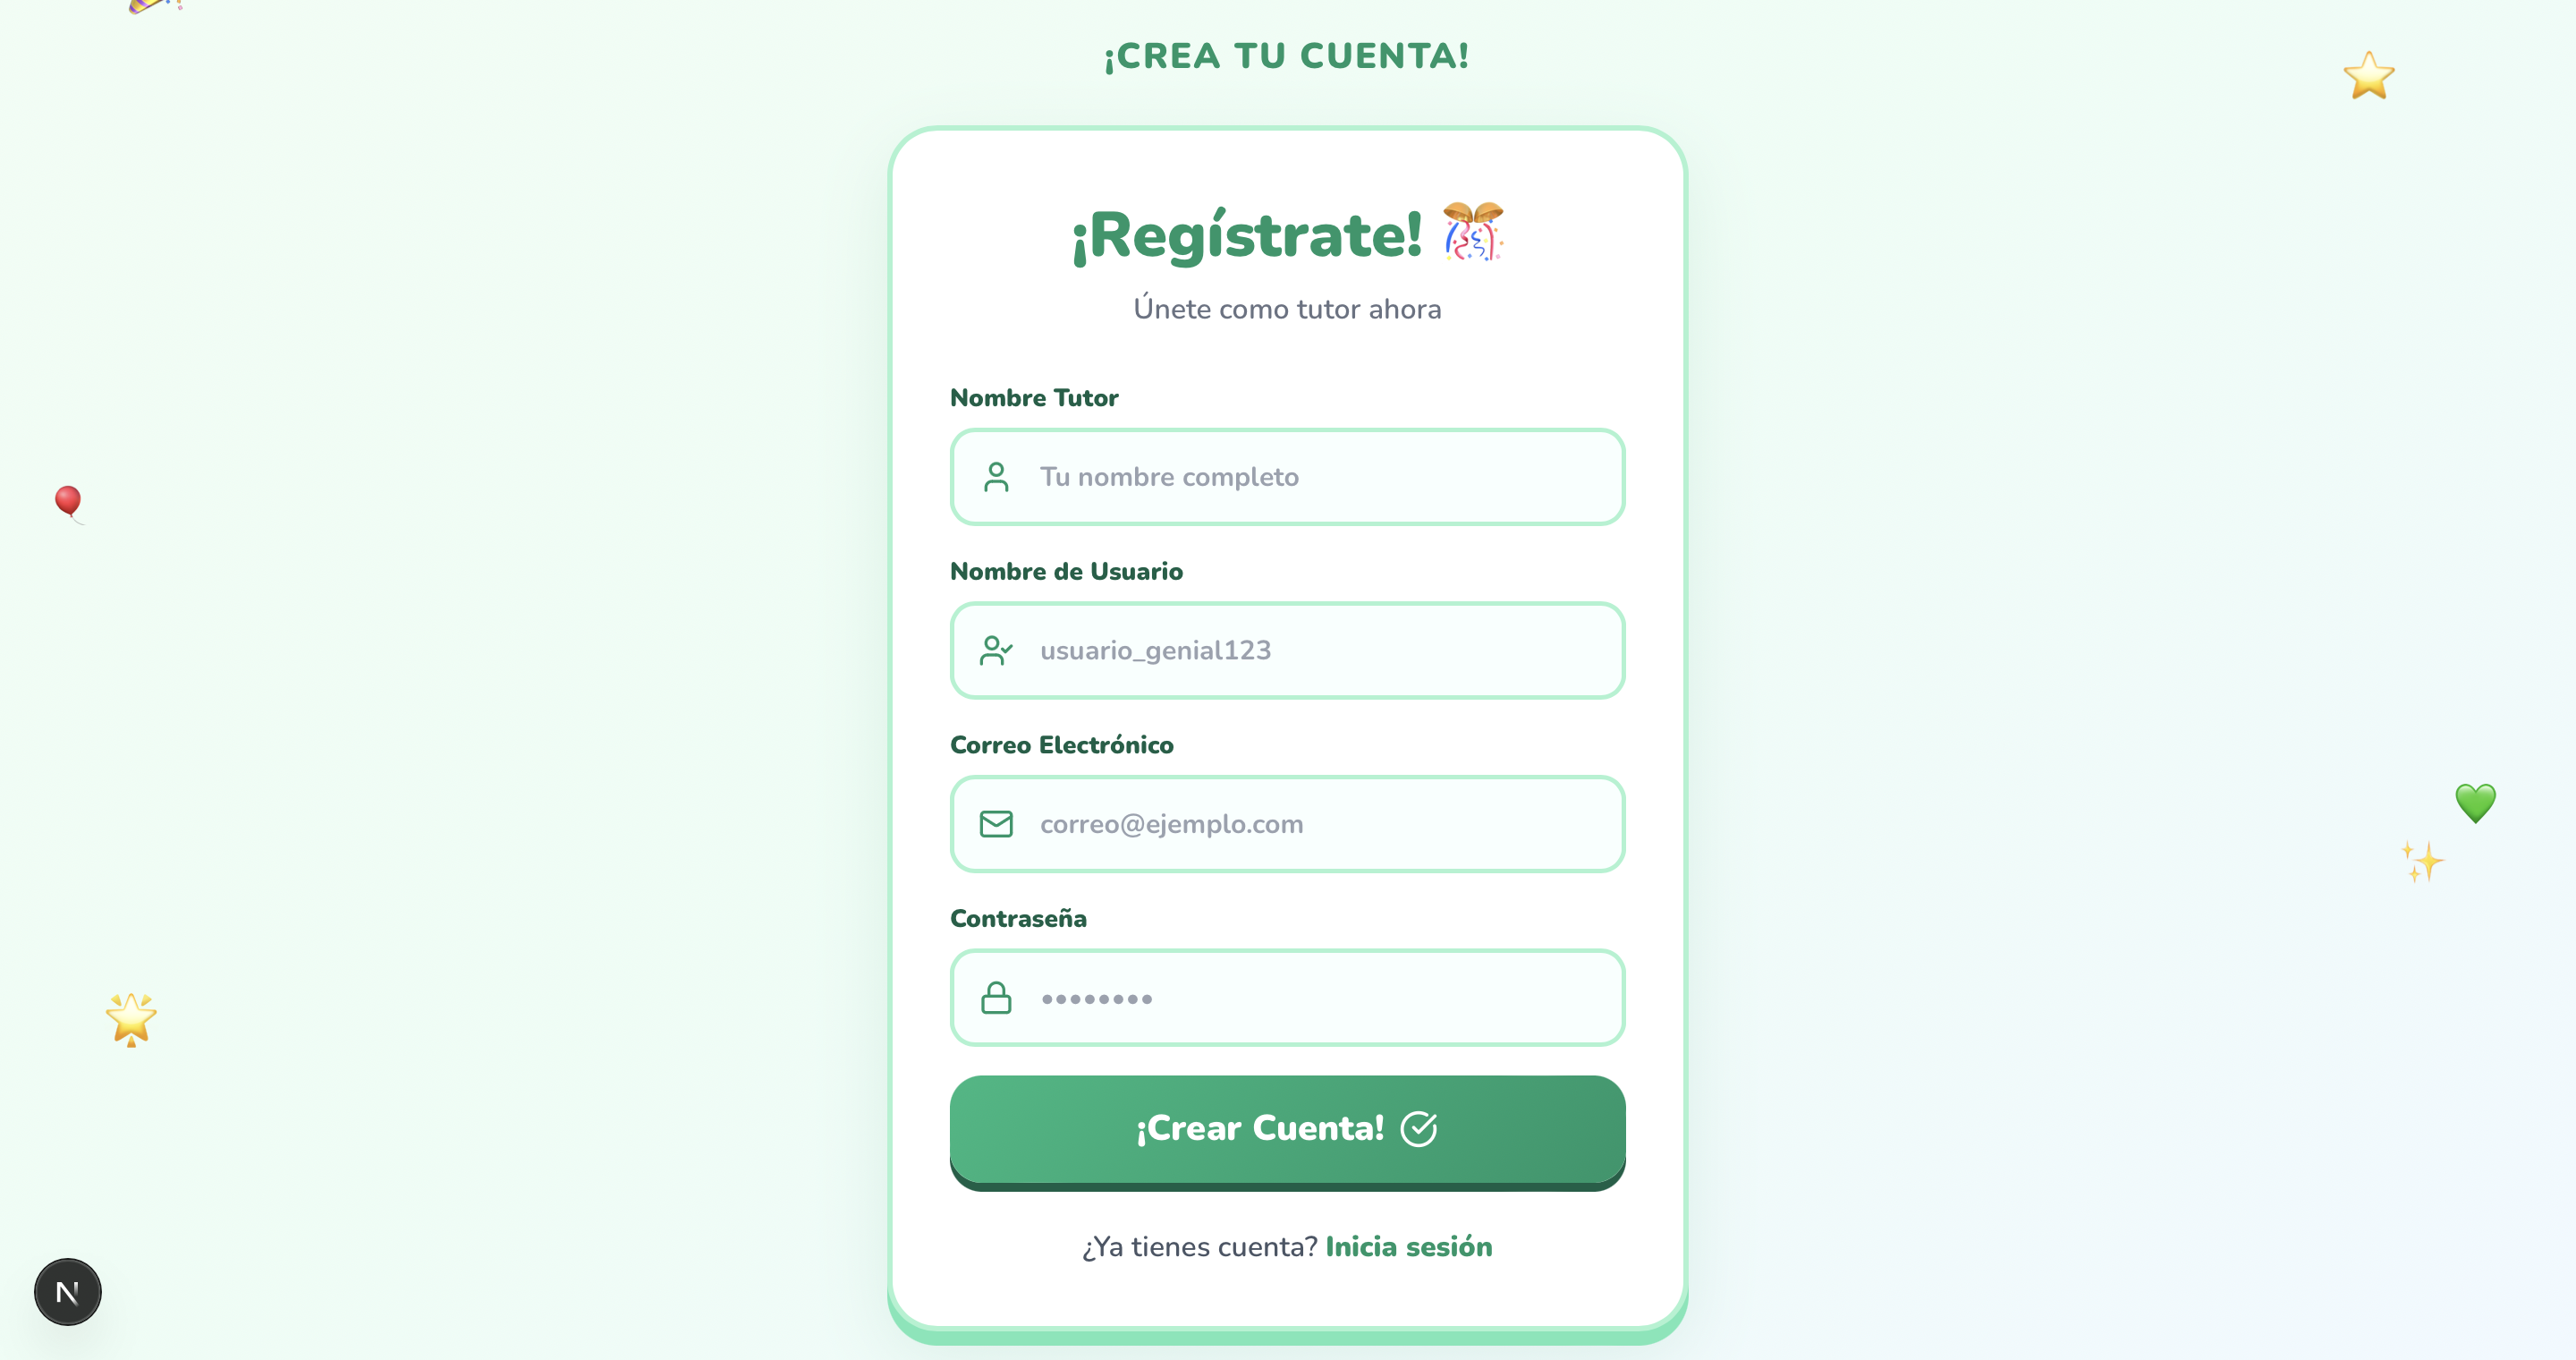
\includegraphics[width=0.7\textwidth]{Imagenes/registrar.png}
    \caption{Registro de nuevo usuario}
    \label{fig:registrar}
\end{figure}

\begin{figure}[H]
    \centering
    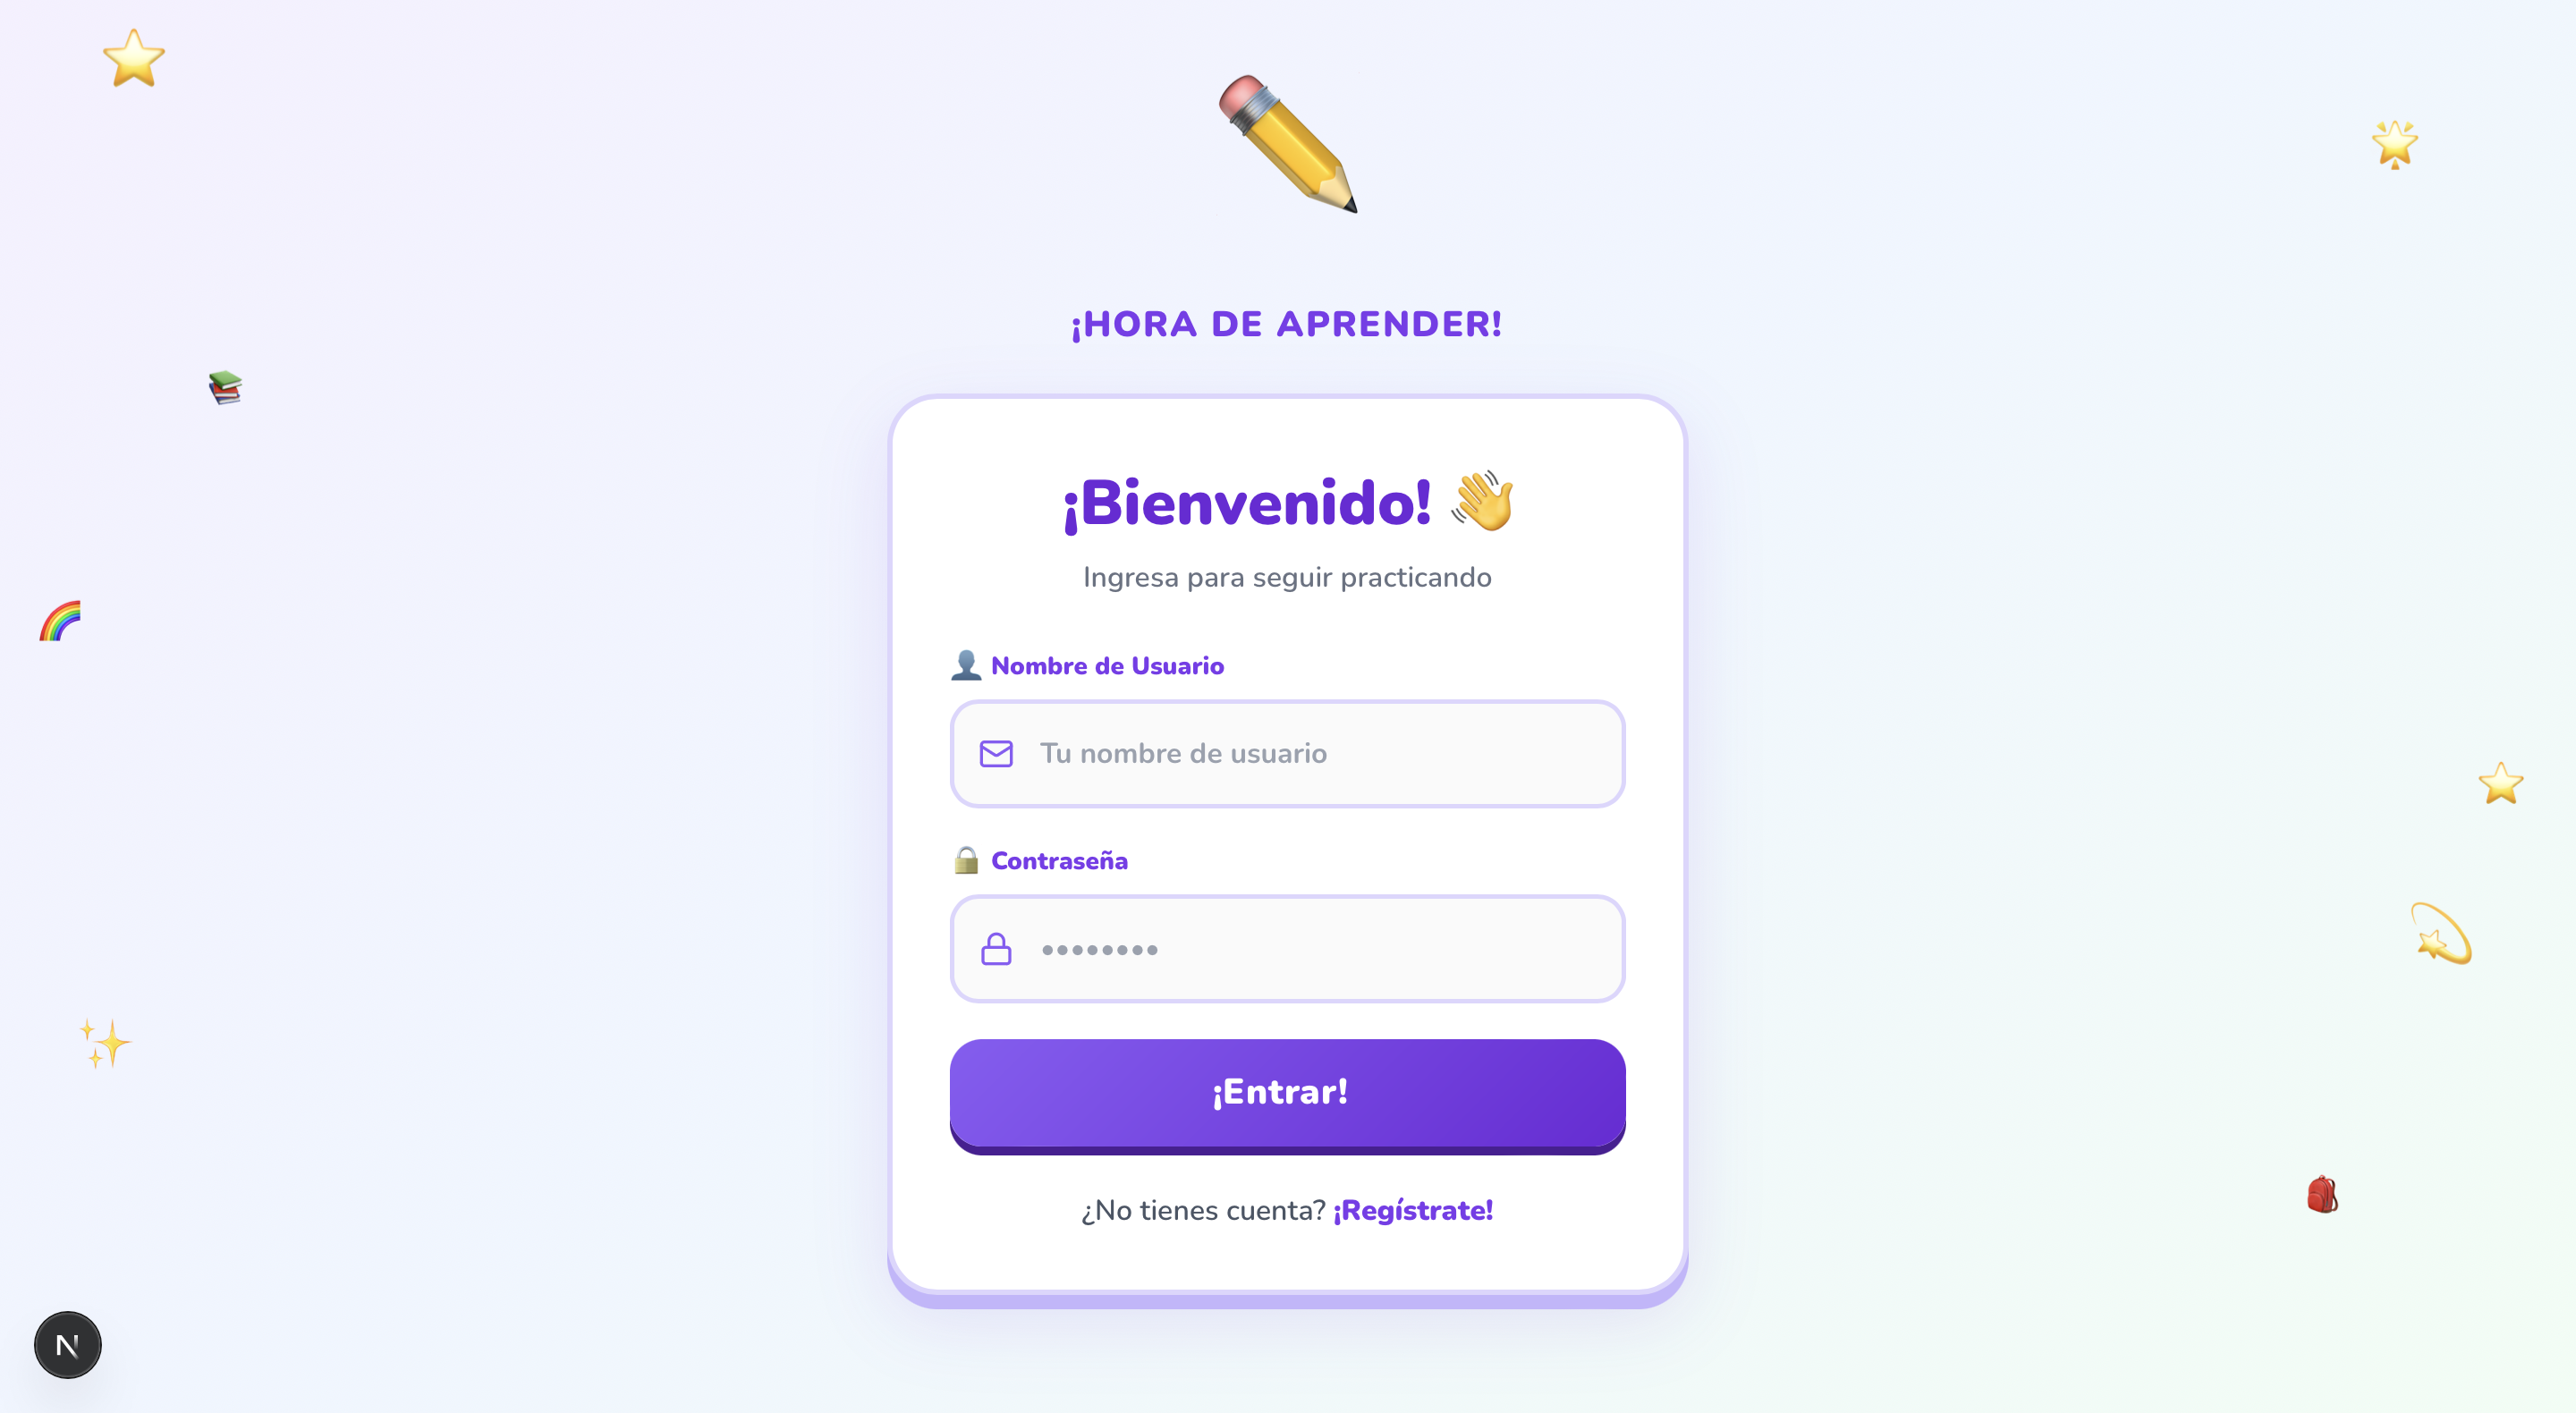
\includegraphics[width=0.7\textwidth]{Imagenes/login.png}
    \caption{Inicio de sesión}
    \label{fig:login}
\end{figure}

\subsubsection{Vistas del tutor}

\begin{figure}[H]
    \centering
    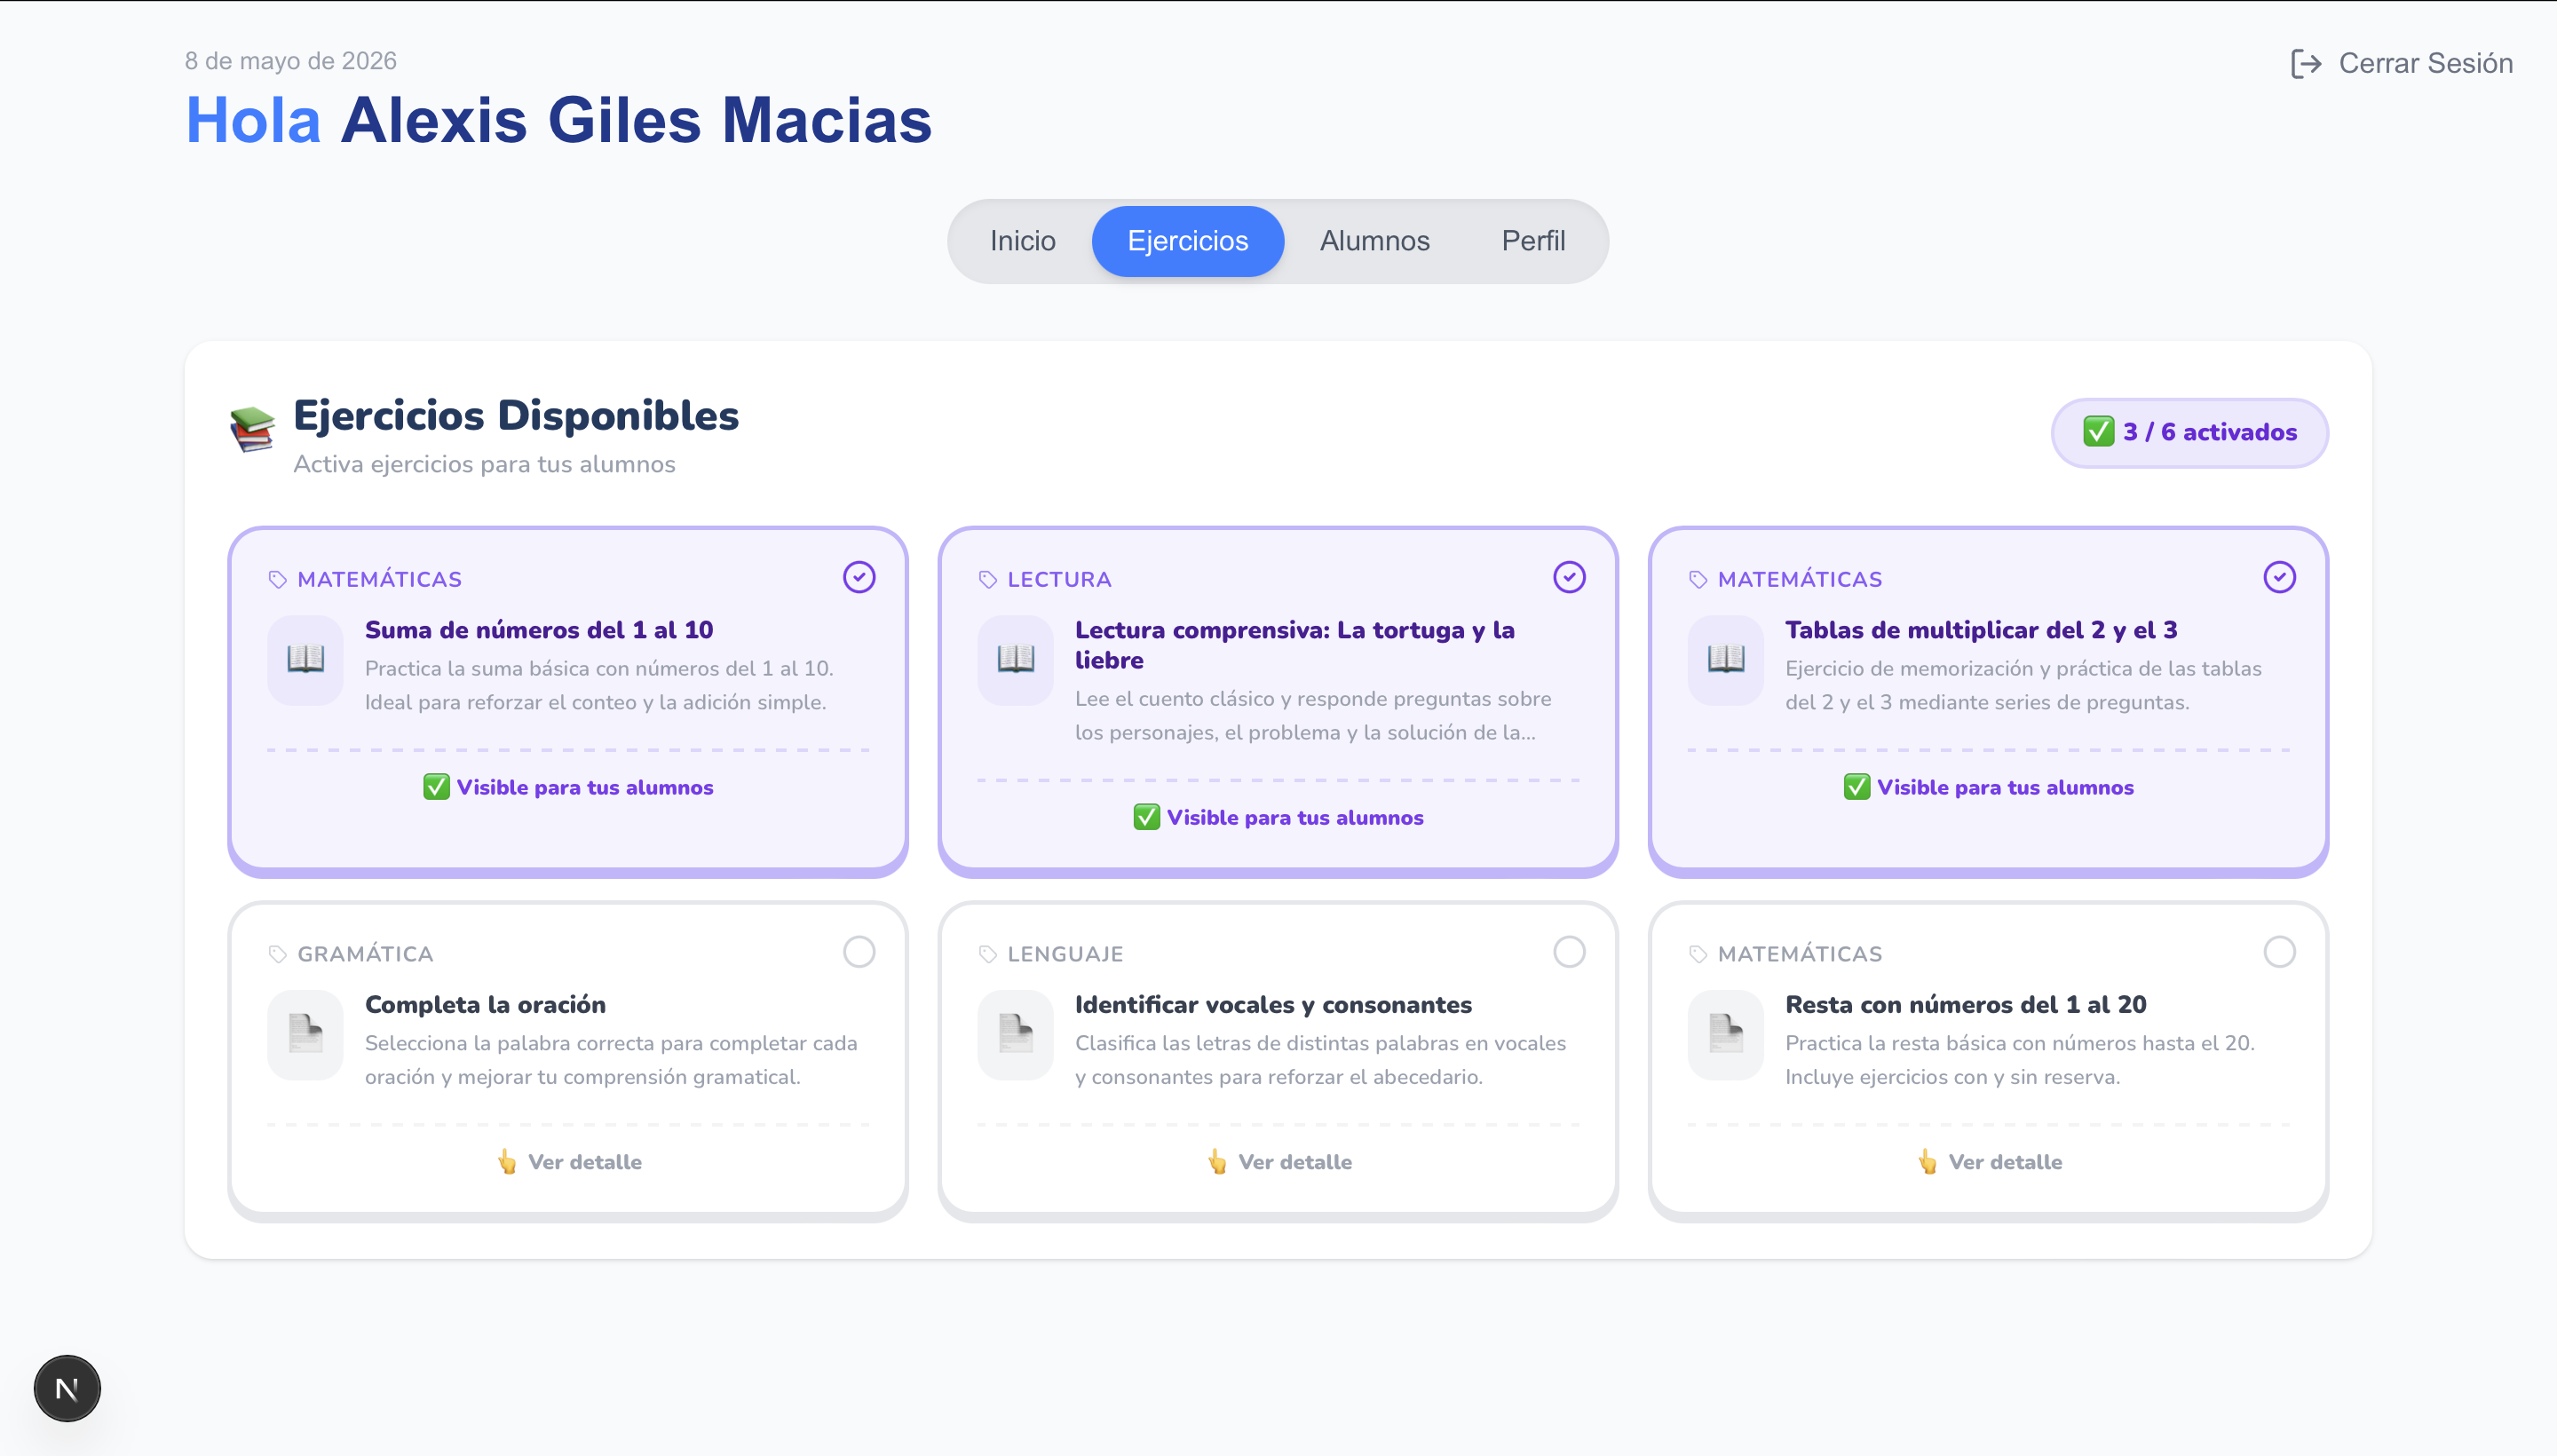
\includegraphics[width=0.7\textwidth]{Imagenes/EjerciciosTutor.png}
    \caption{Catalogo de ejercicios para tutor y ejercicios}
    \label{fig:ejeTu}
\end{figure}

\begin{figure}[H]
    \centering
    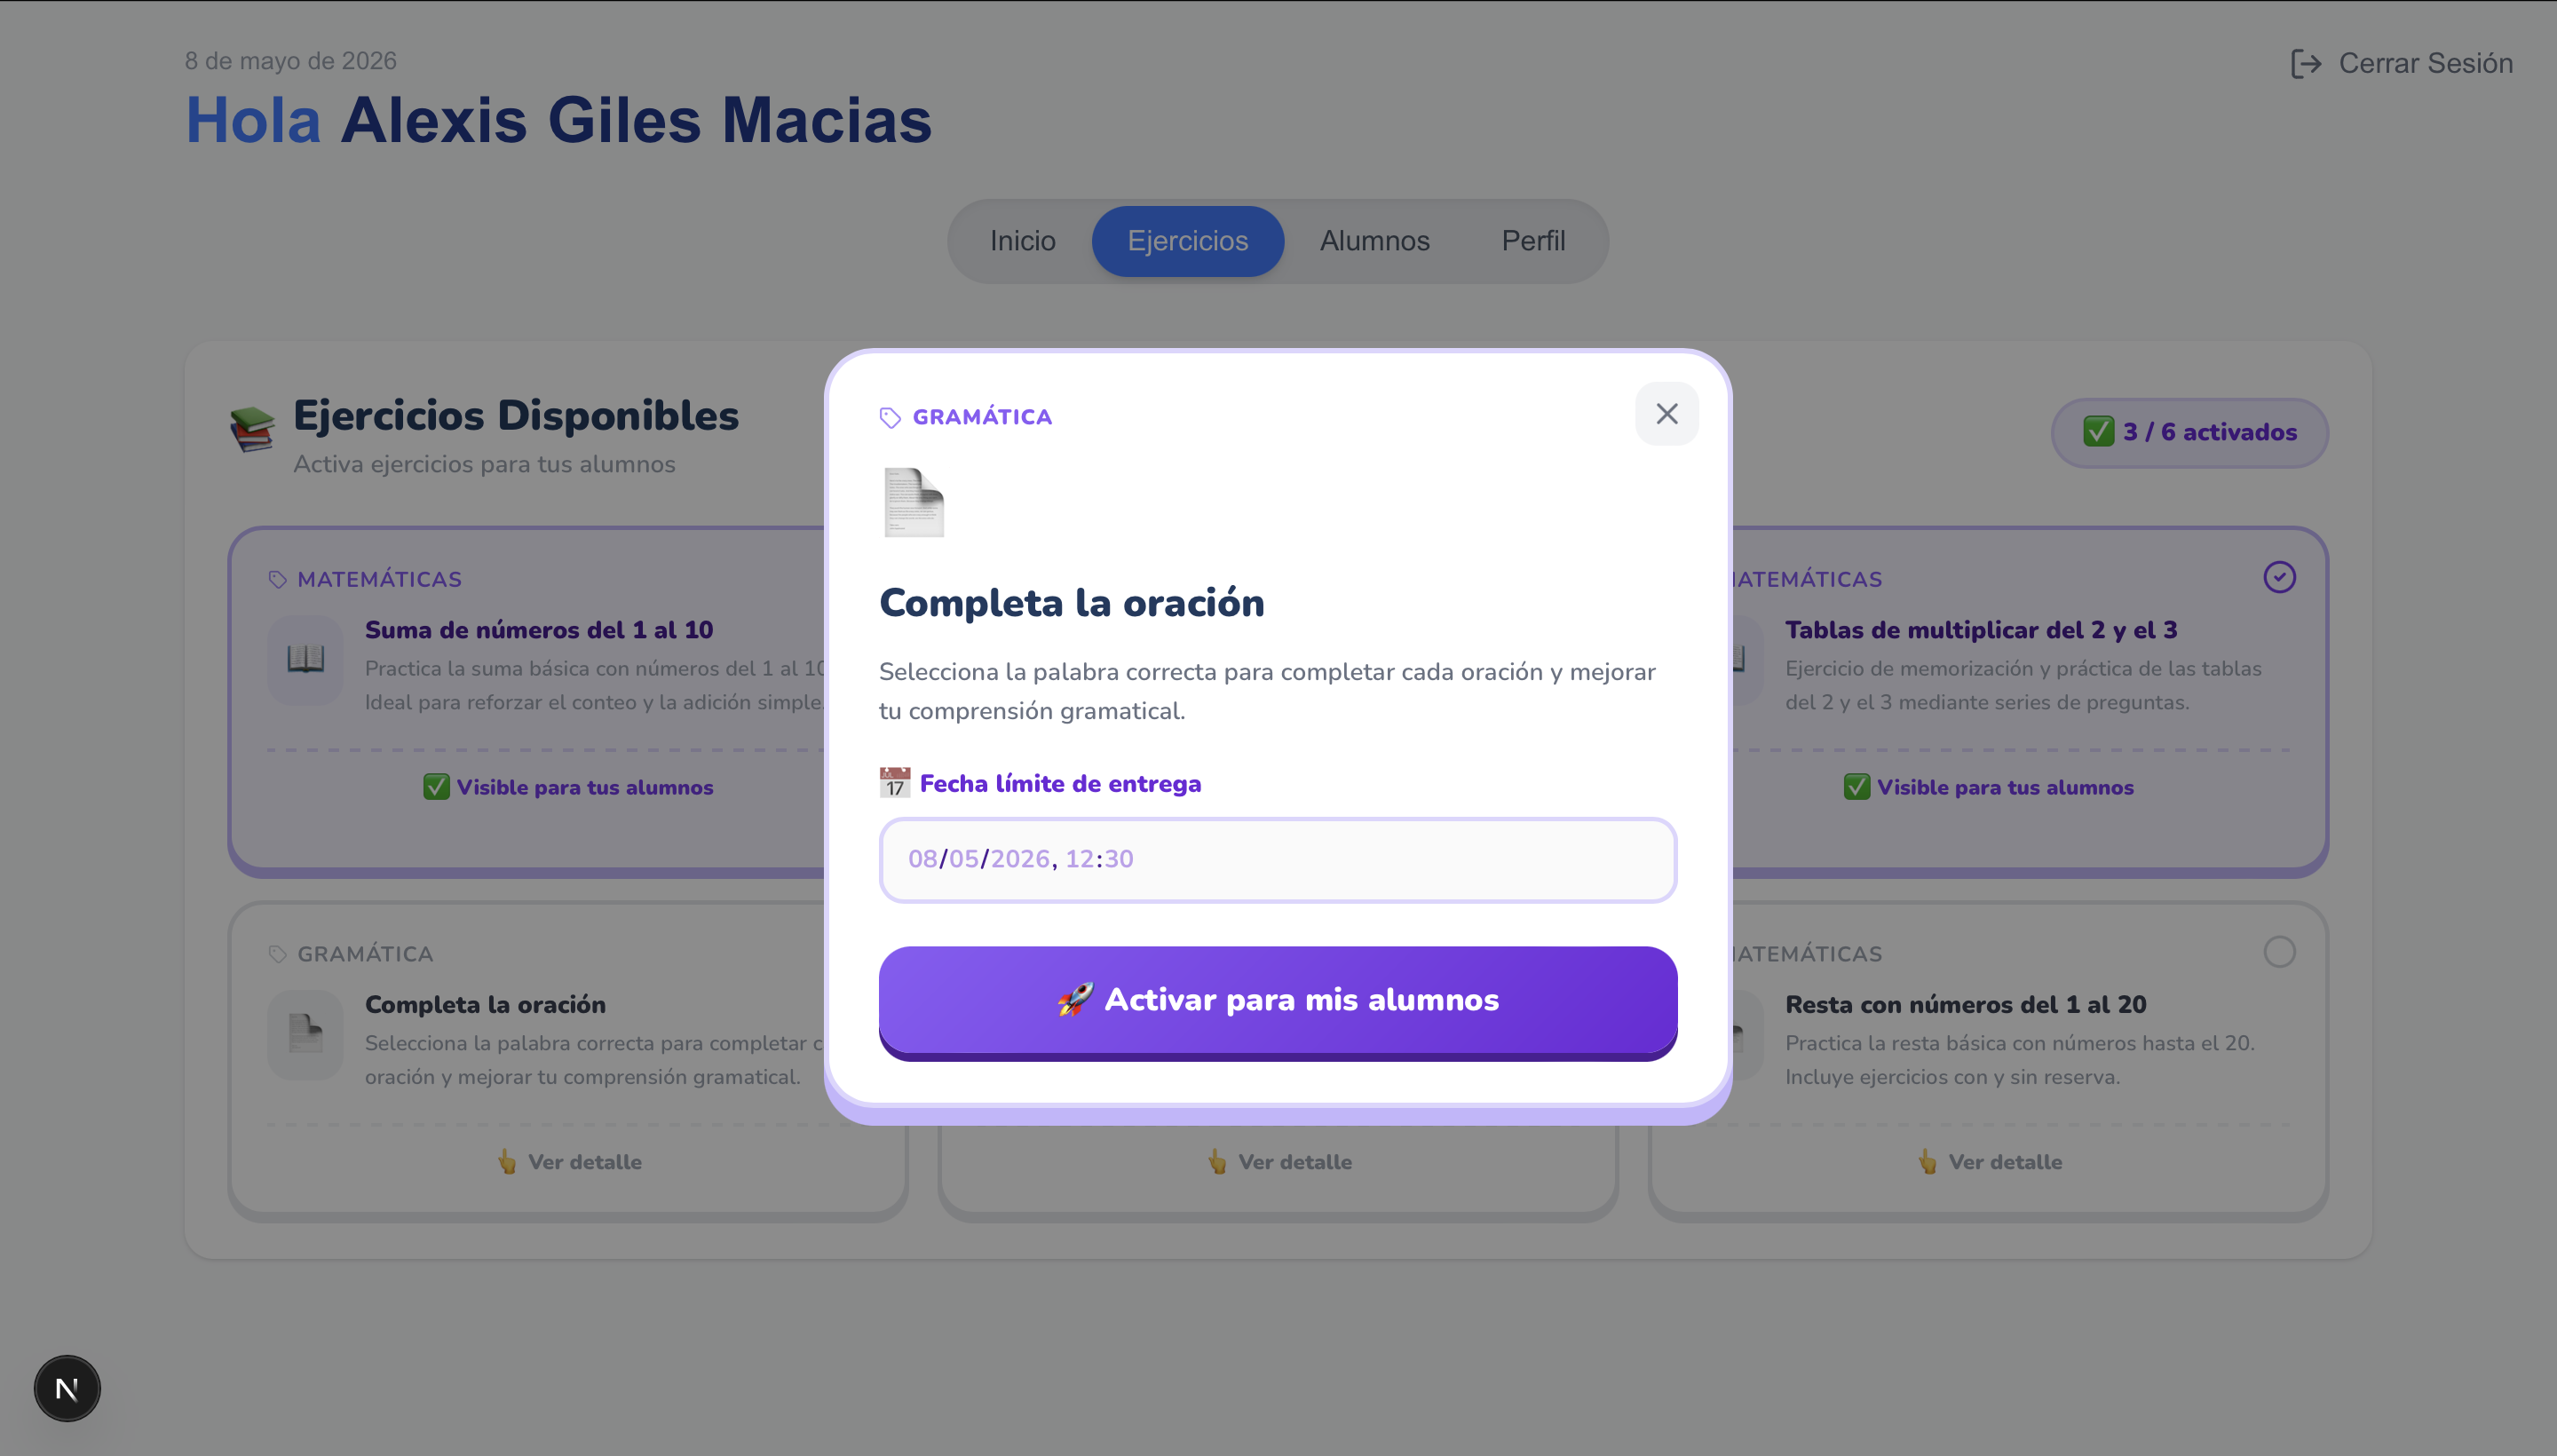
\includegraphics[width=0.7\textwidth]{Imagenes/asignacion.png}
    \caption{Asignacion de ejercicios a alumnos}
    \label{fig:asignacionEje}
\end{figure}

\begin{figure}[H]
    \centering
    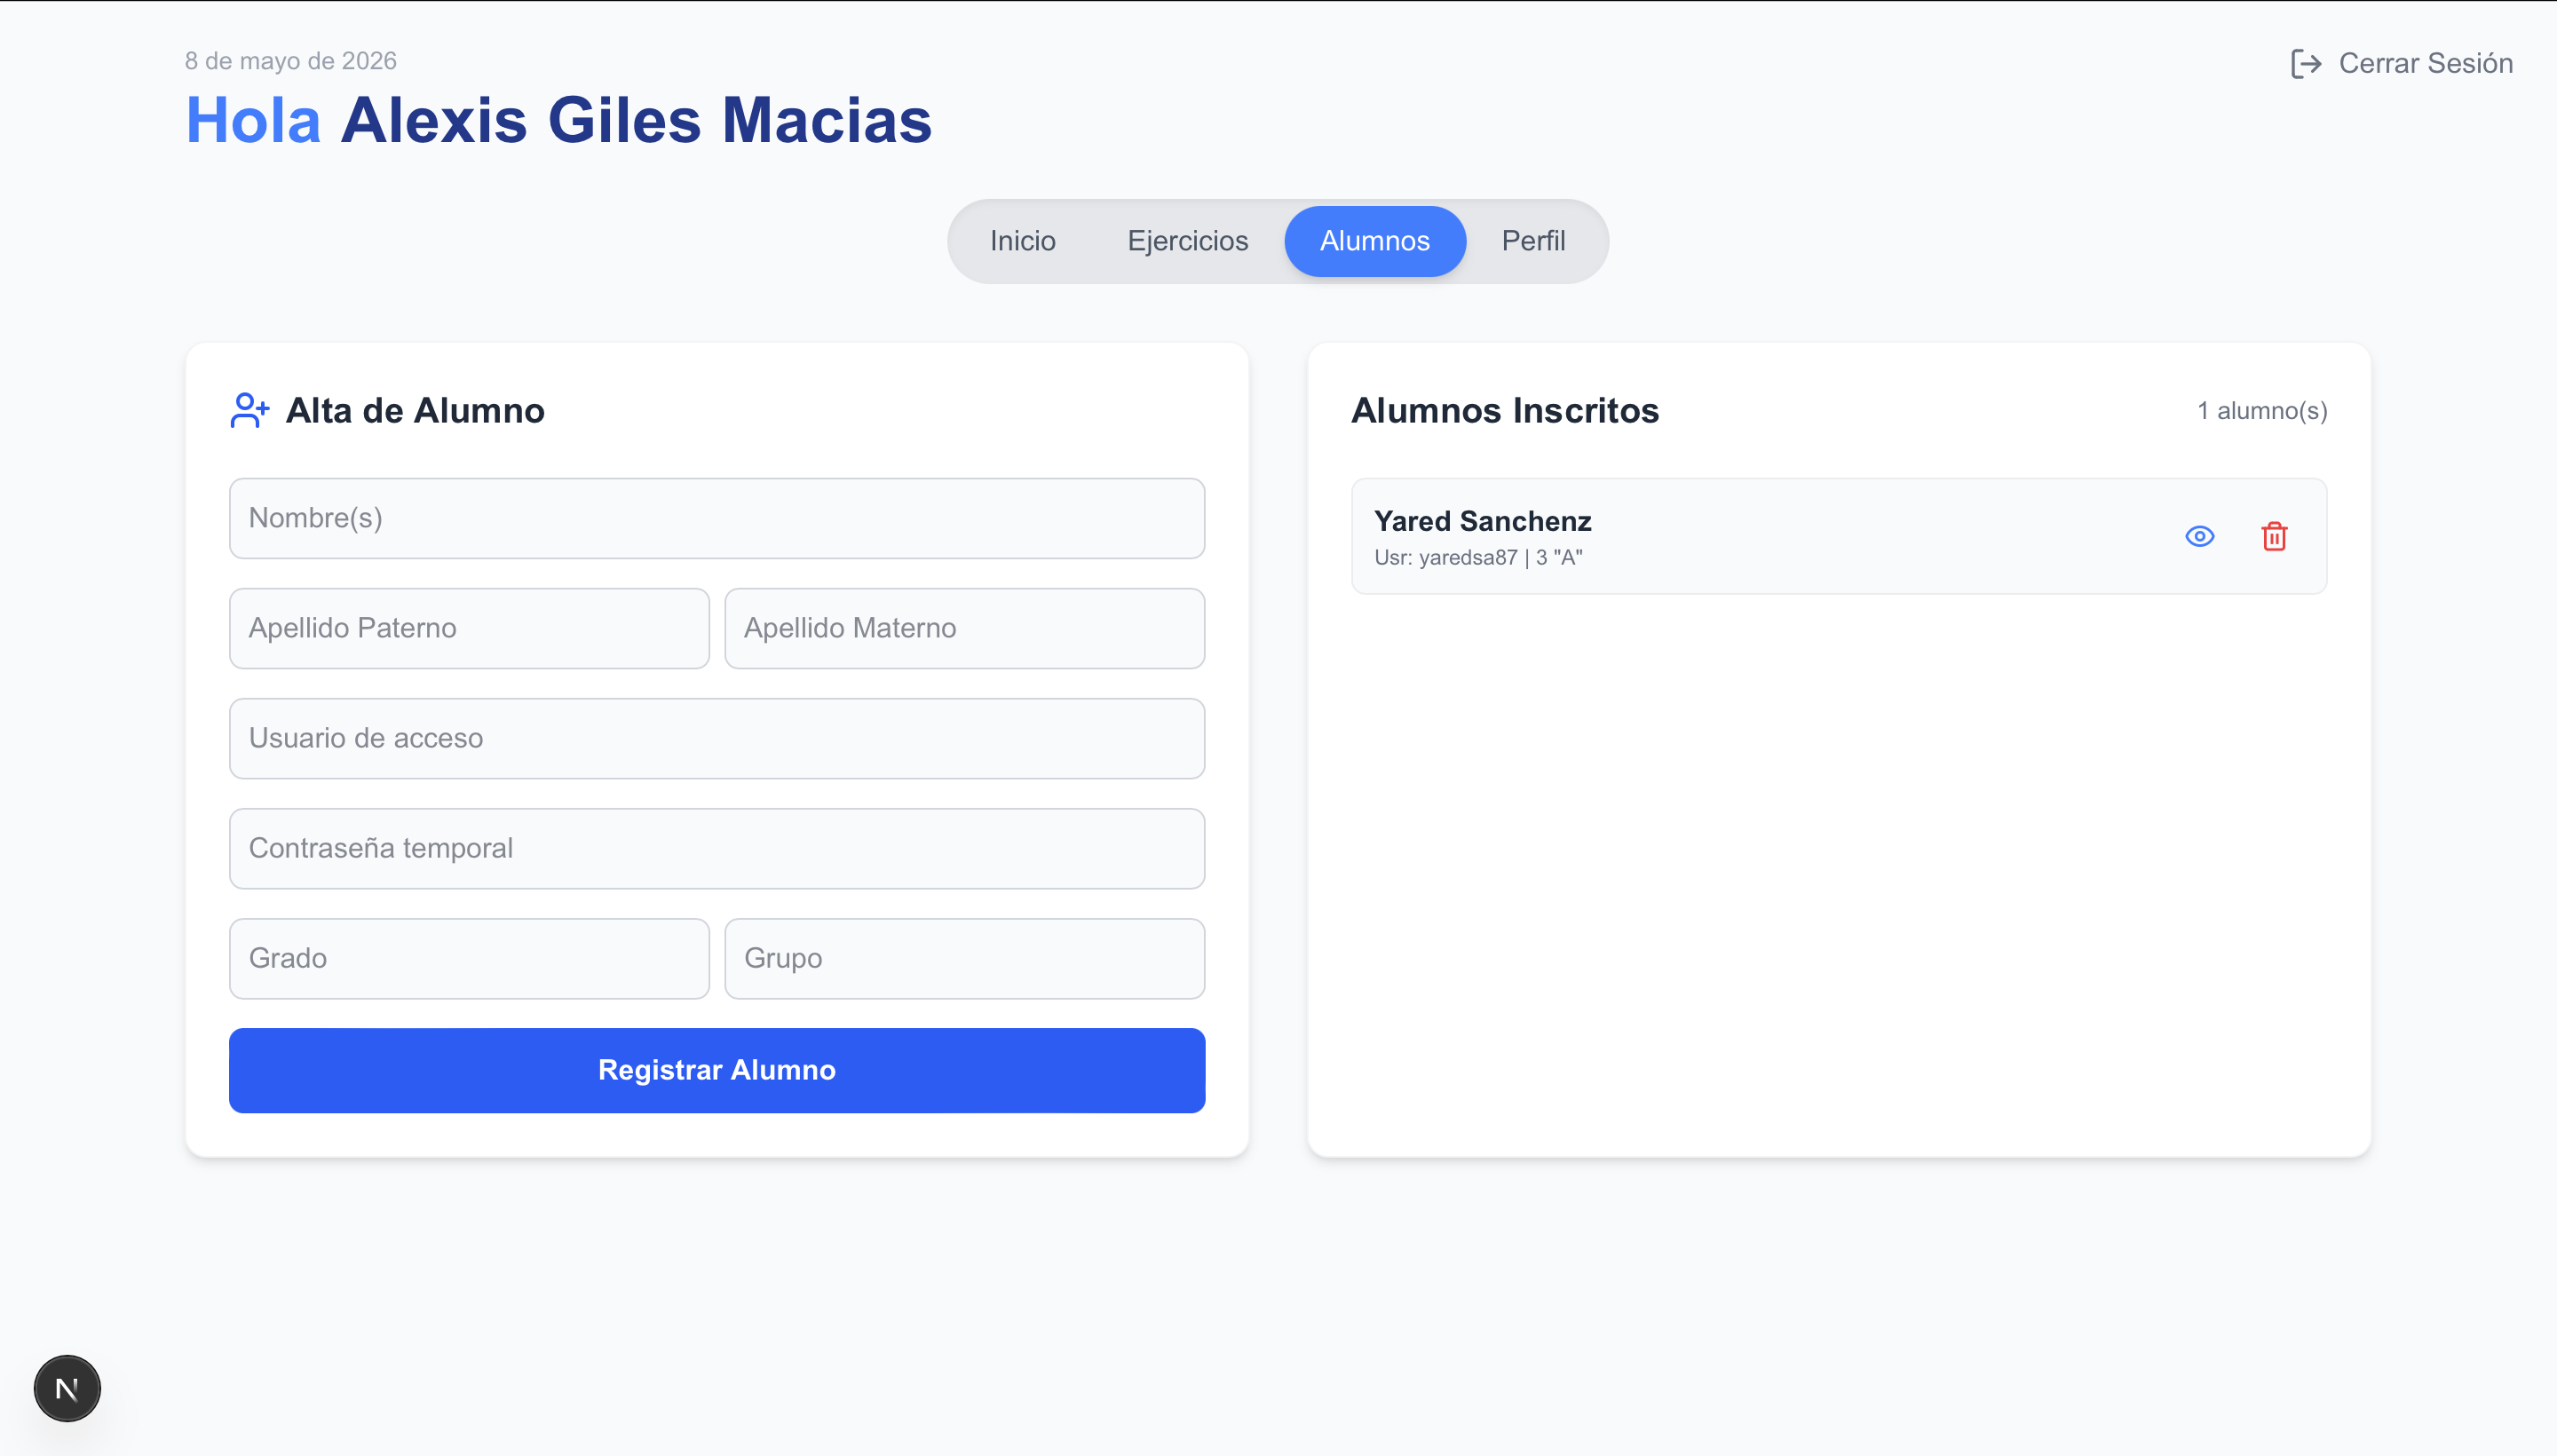
\includegraphics[width=0.7\textwidth]{Imagenes/AlumnosInscritos.png}
    \caption{Alta de alumnos y visualización de alumnos inscritos}
    \label{fig:alumnosInscritos}
\end{figure}

\begin{figure}[H]
    \centering
    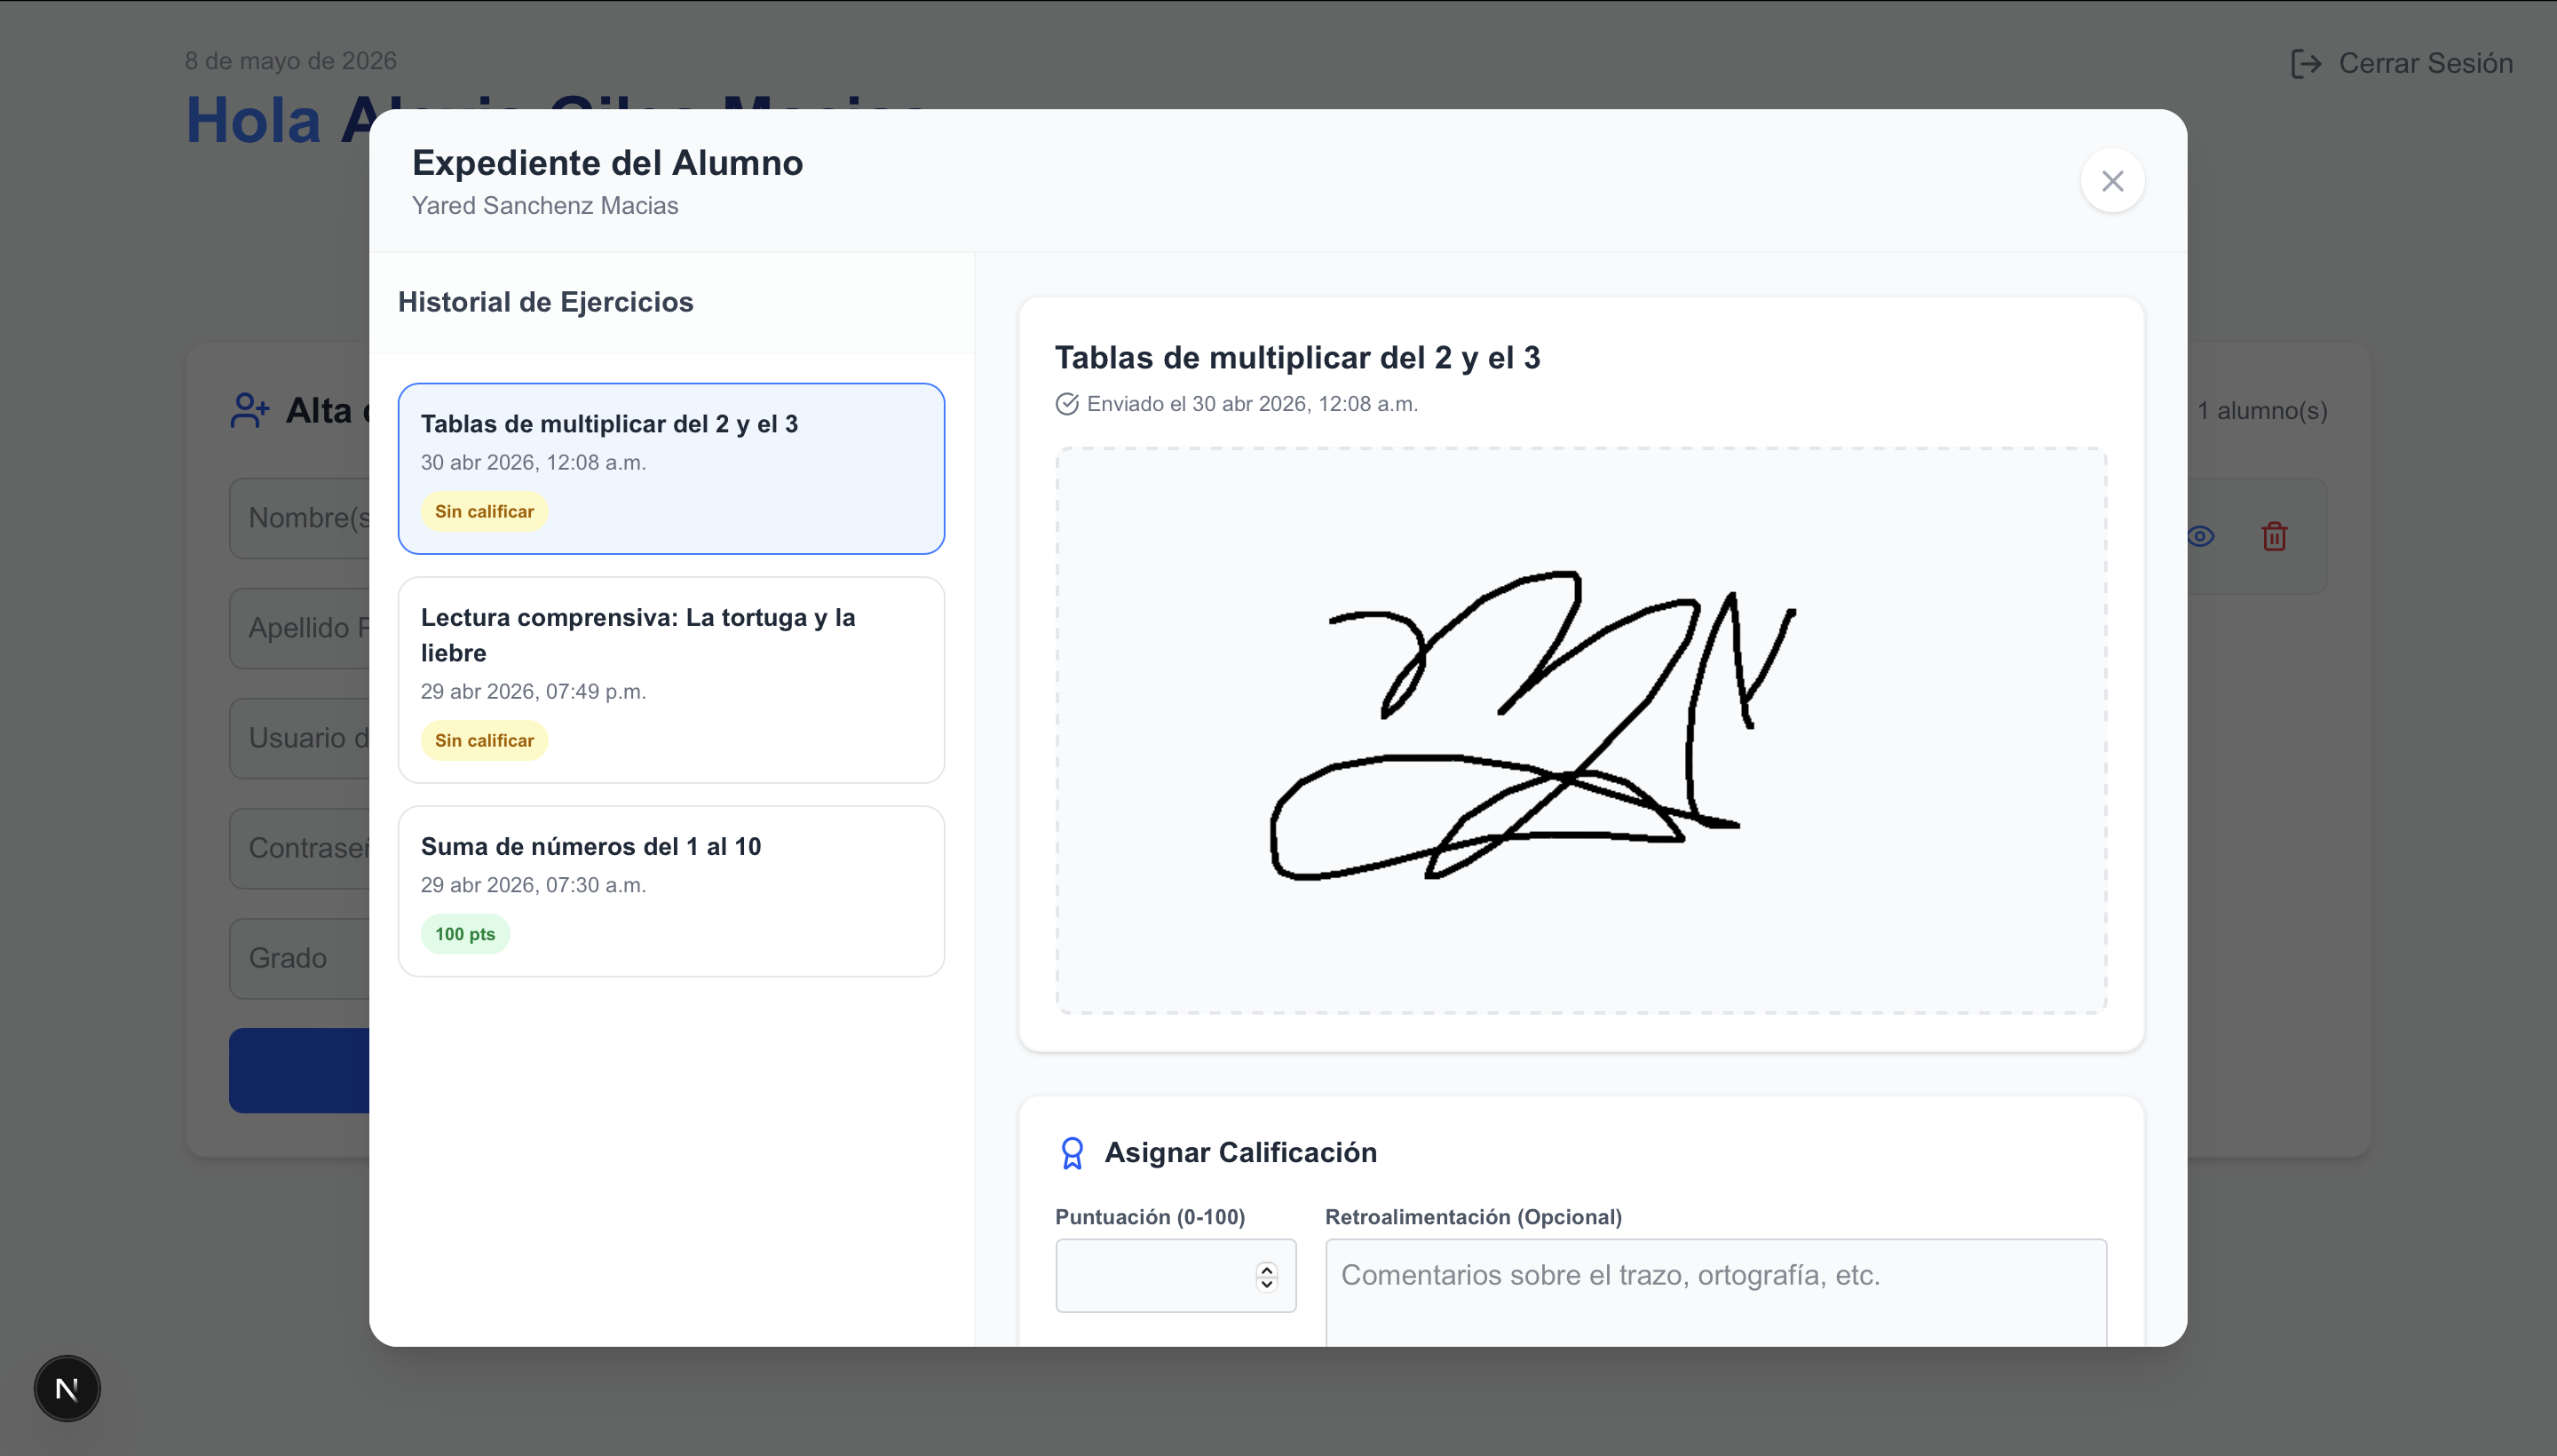
\includegraphics[width=0.7\textwidth]{Imagenes/historialAlumnos.png}
    \caption{Visualizacion del historial de ejercicios realizados por los alumnos}
    \label{fig:historialAlumnos}
\end{figure}

\begin{figure}[H]
    \centering
    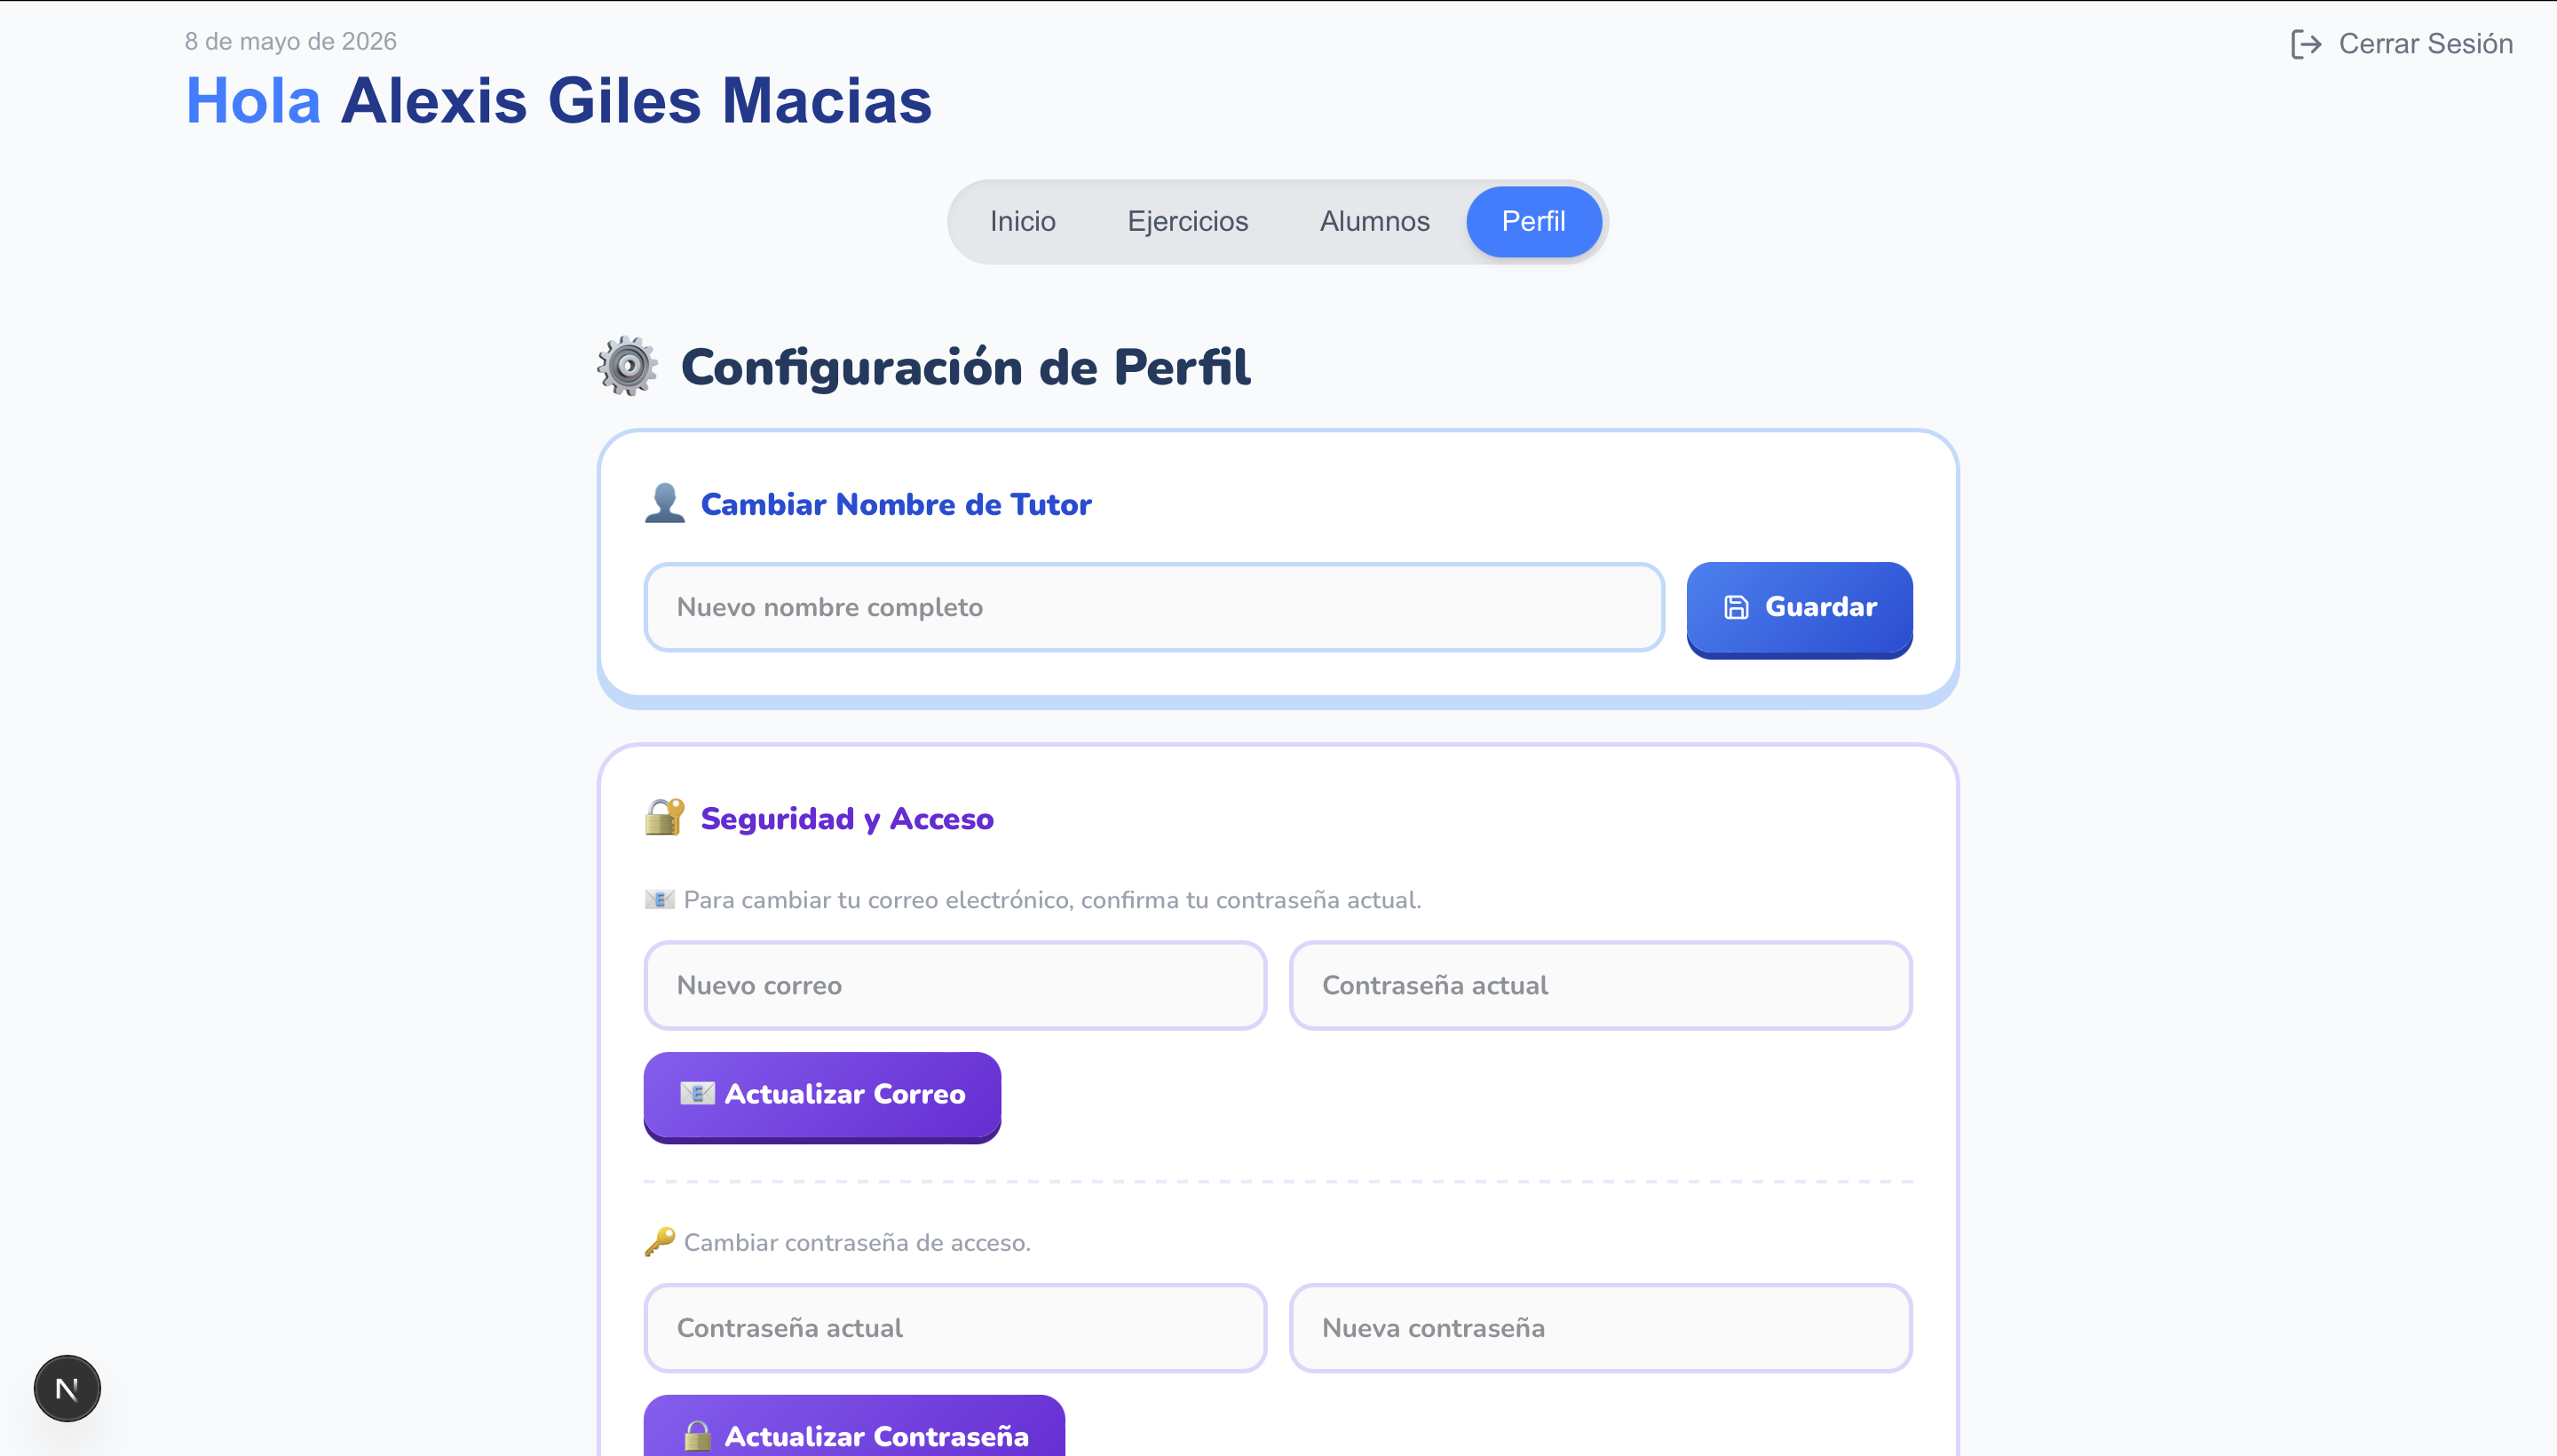
\includegraphics[width=0.7\textwidth]{Imagenes/miperfil.png}
    \caption{Visualizacion del perfil del tutor}
    \label{fig:miperfilT}
\end{figure}

\subsubsection{Vistas del alumno}

\begin{figure}[H]
    \centering
    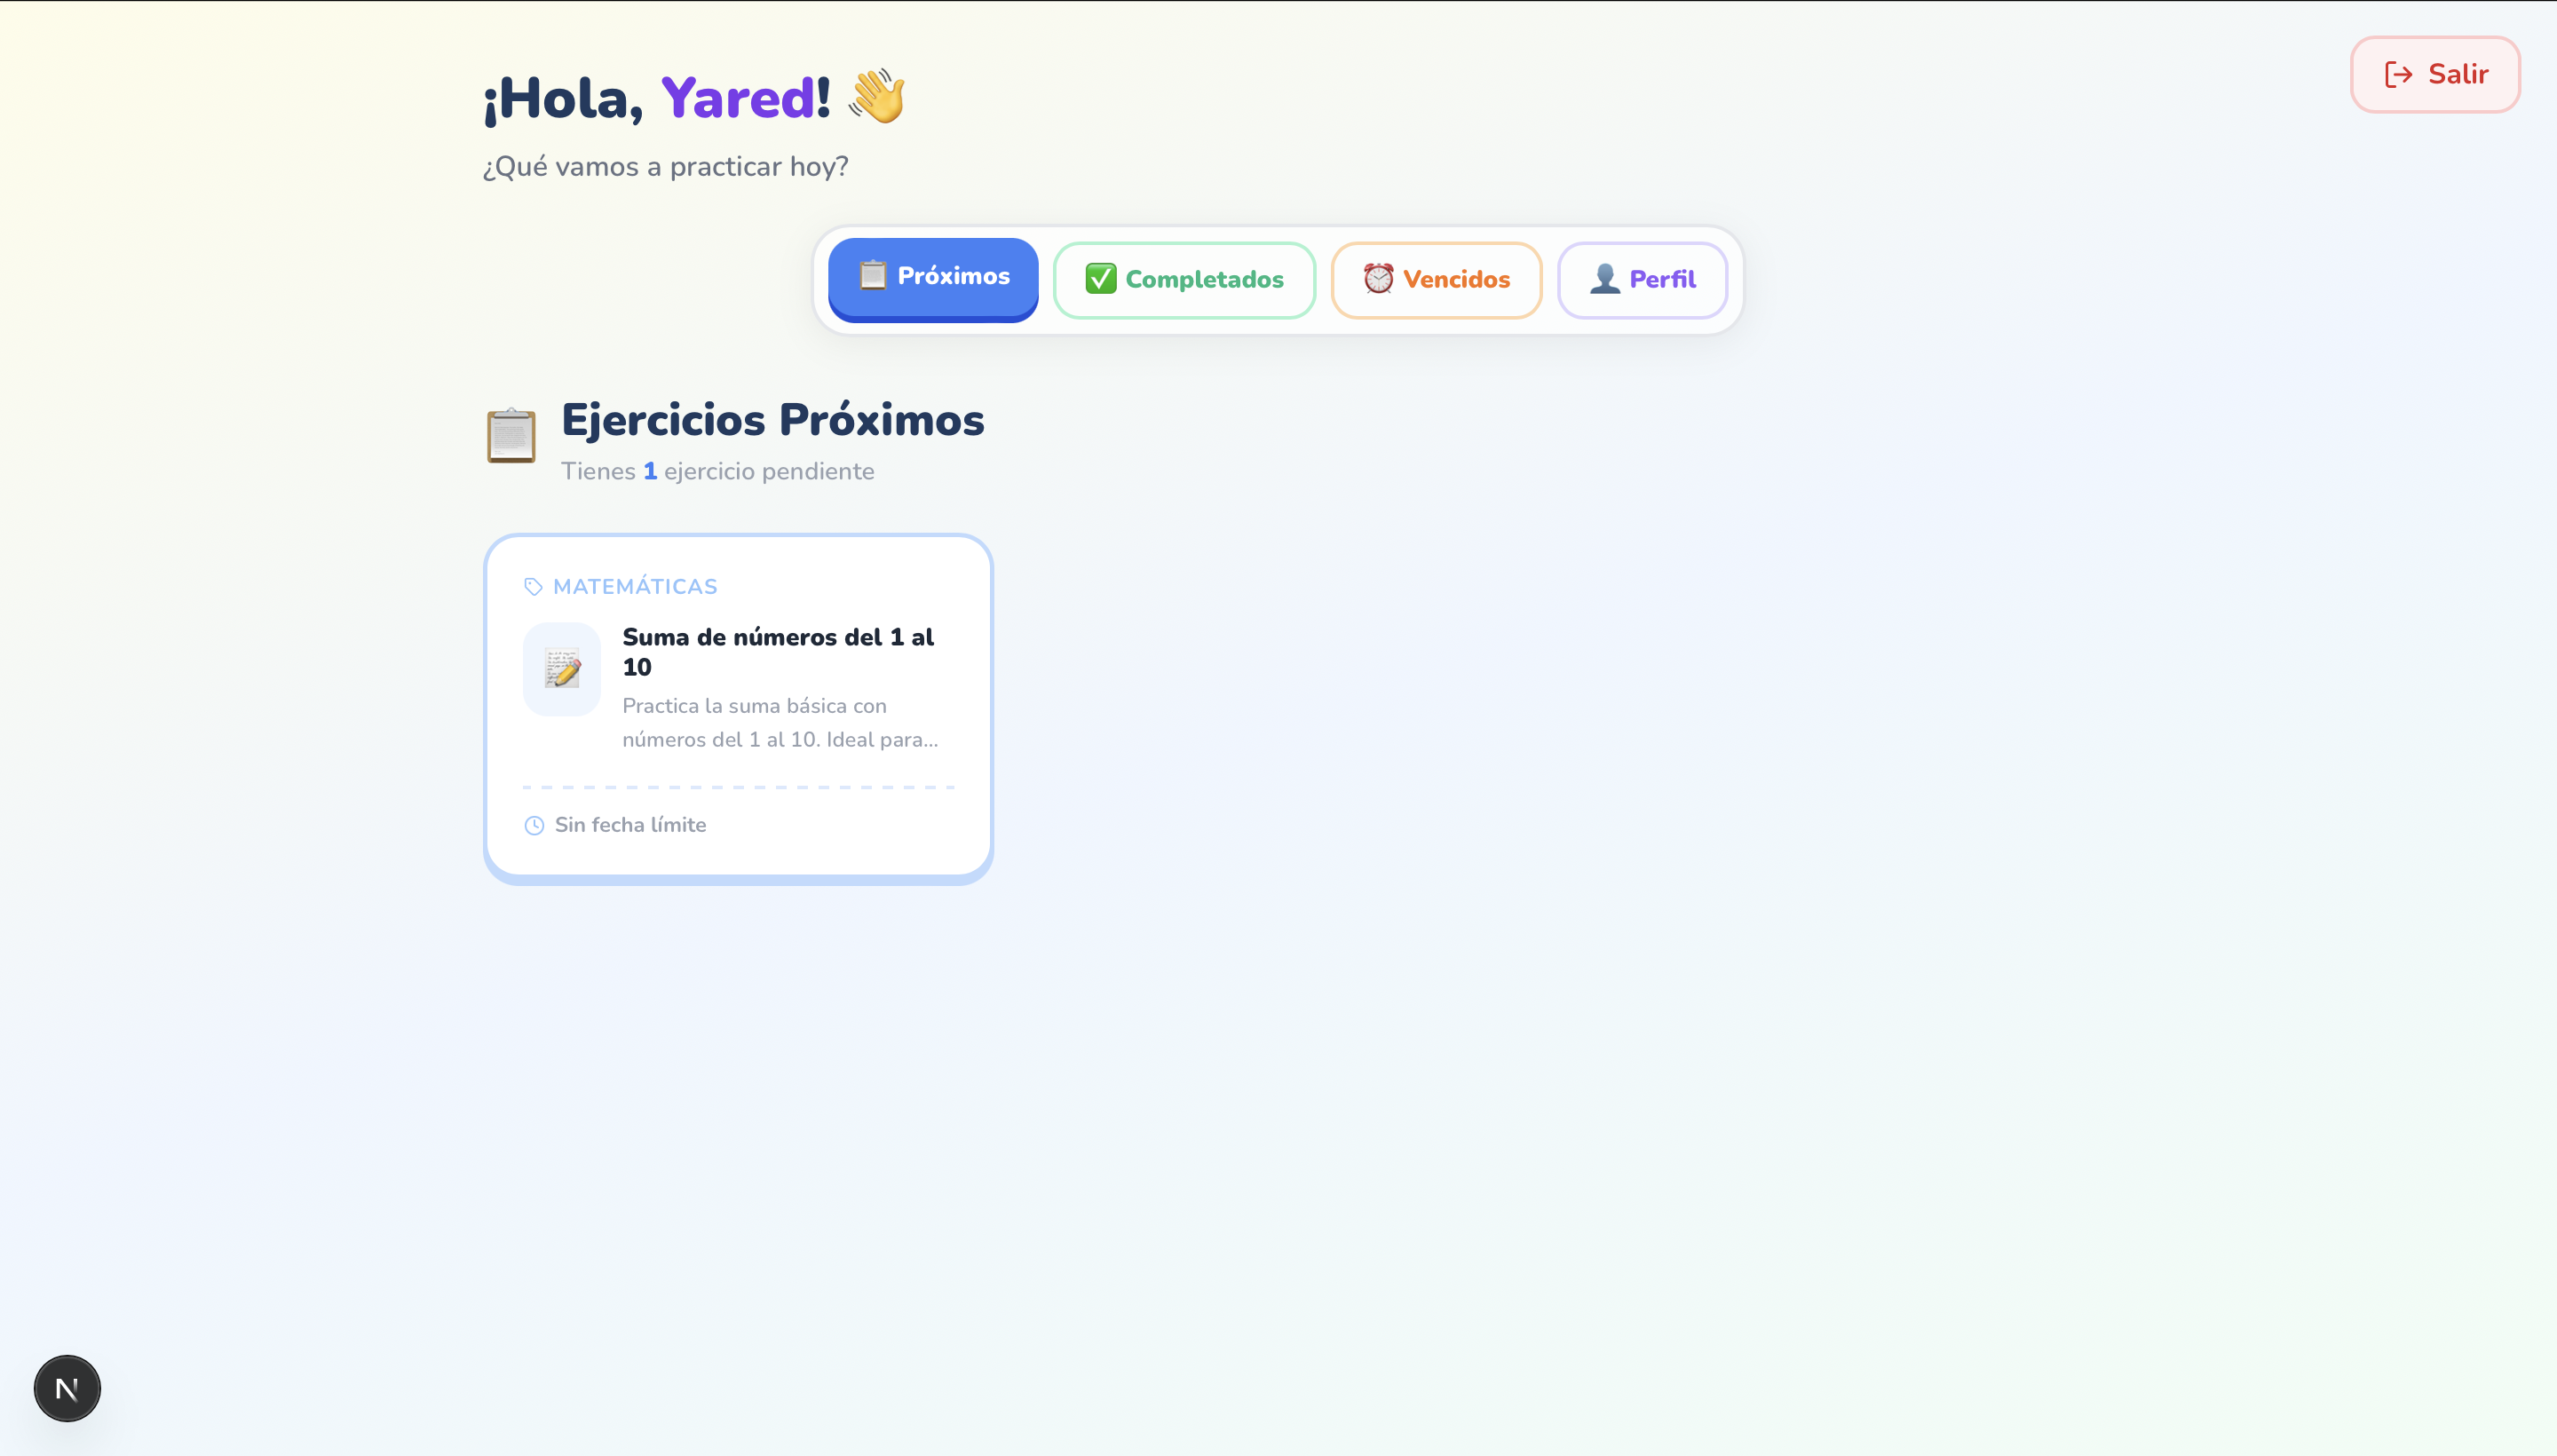
\includegraphics[width=0.7\textwidth]{Imagenes/ejerciciosProximos.png}
    \caption{Visualización de ejercicios próximos a vencer}
    \label{fig:ejerciciosProximos}
\end{figure}

\begin{figure}[H]
    \centering
    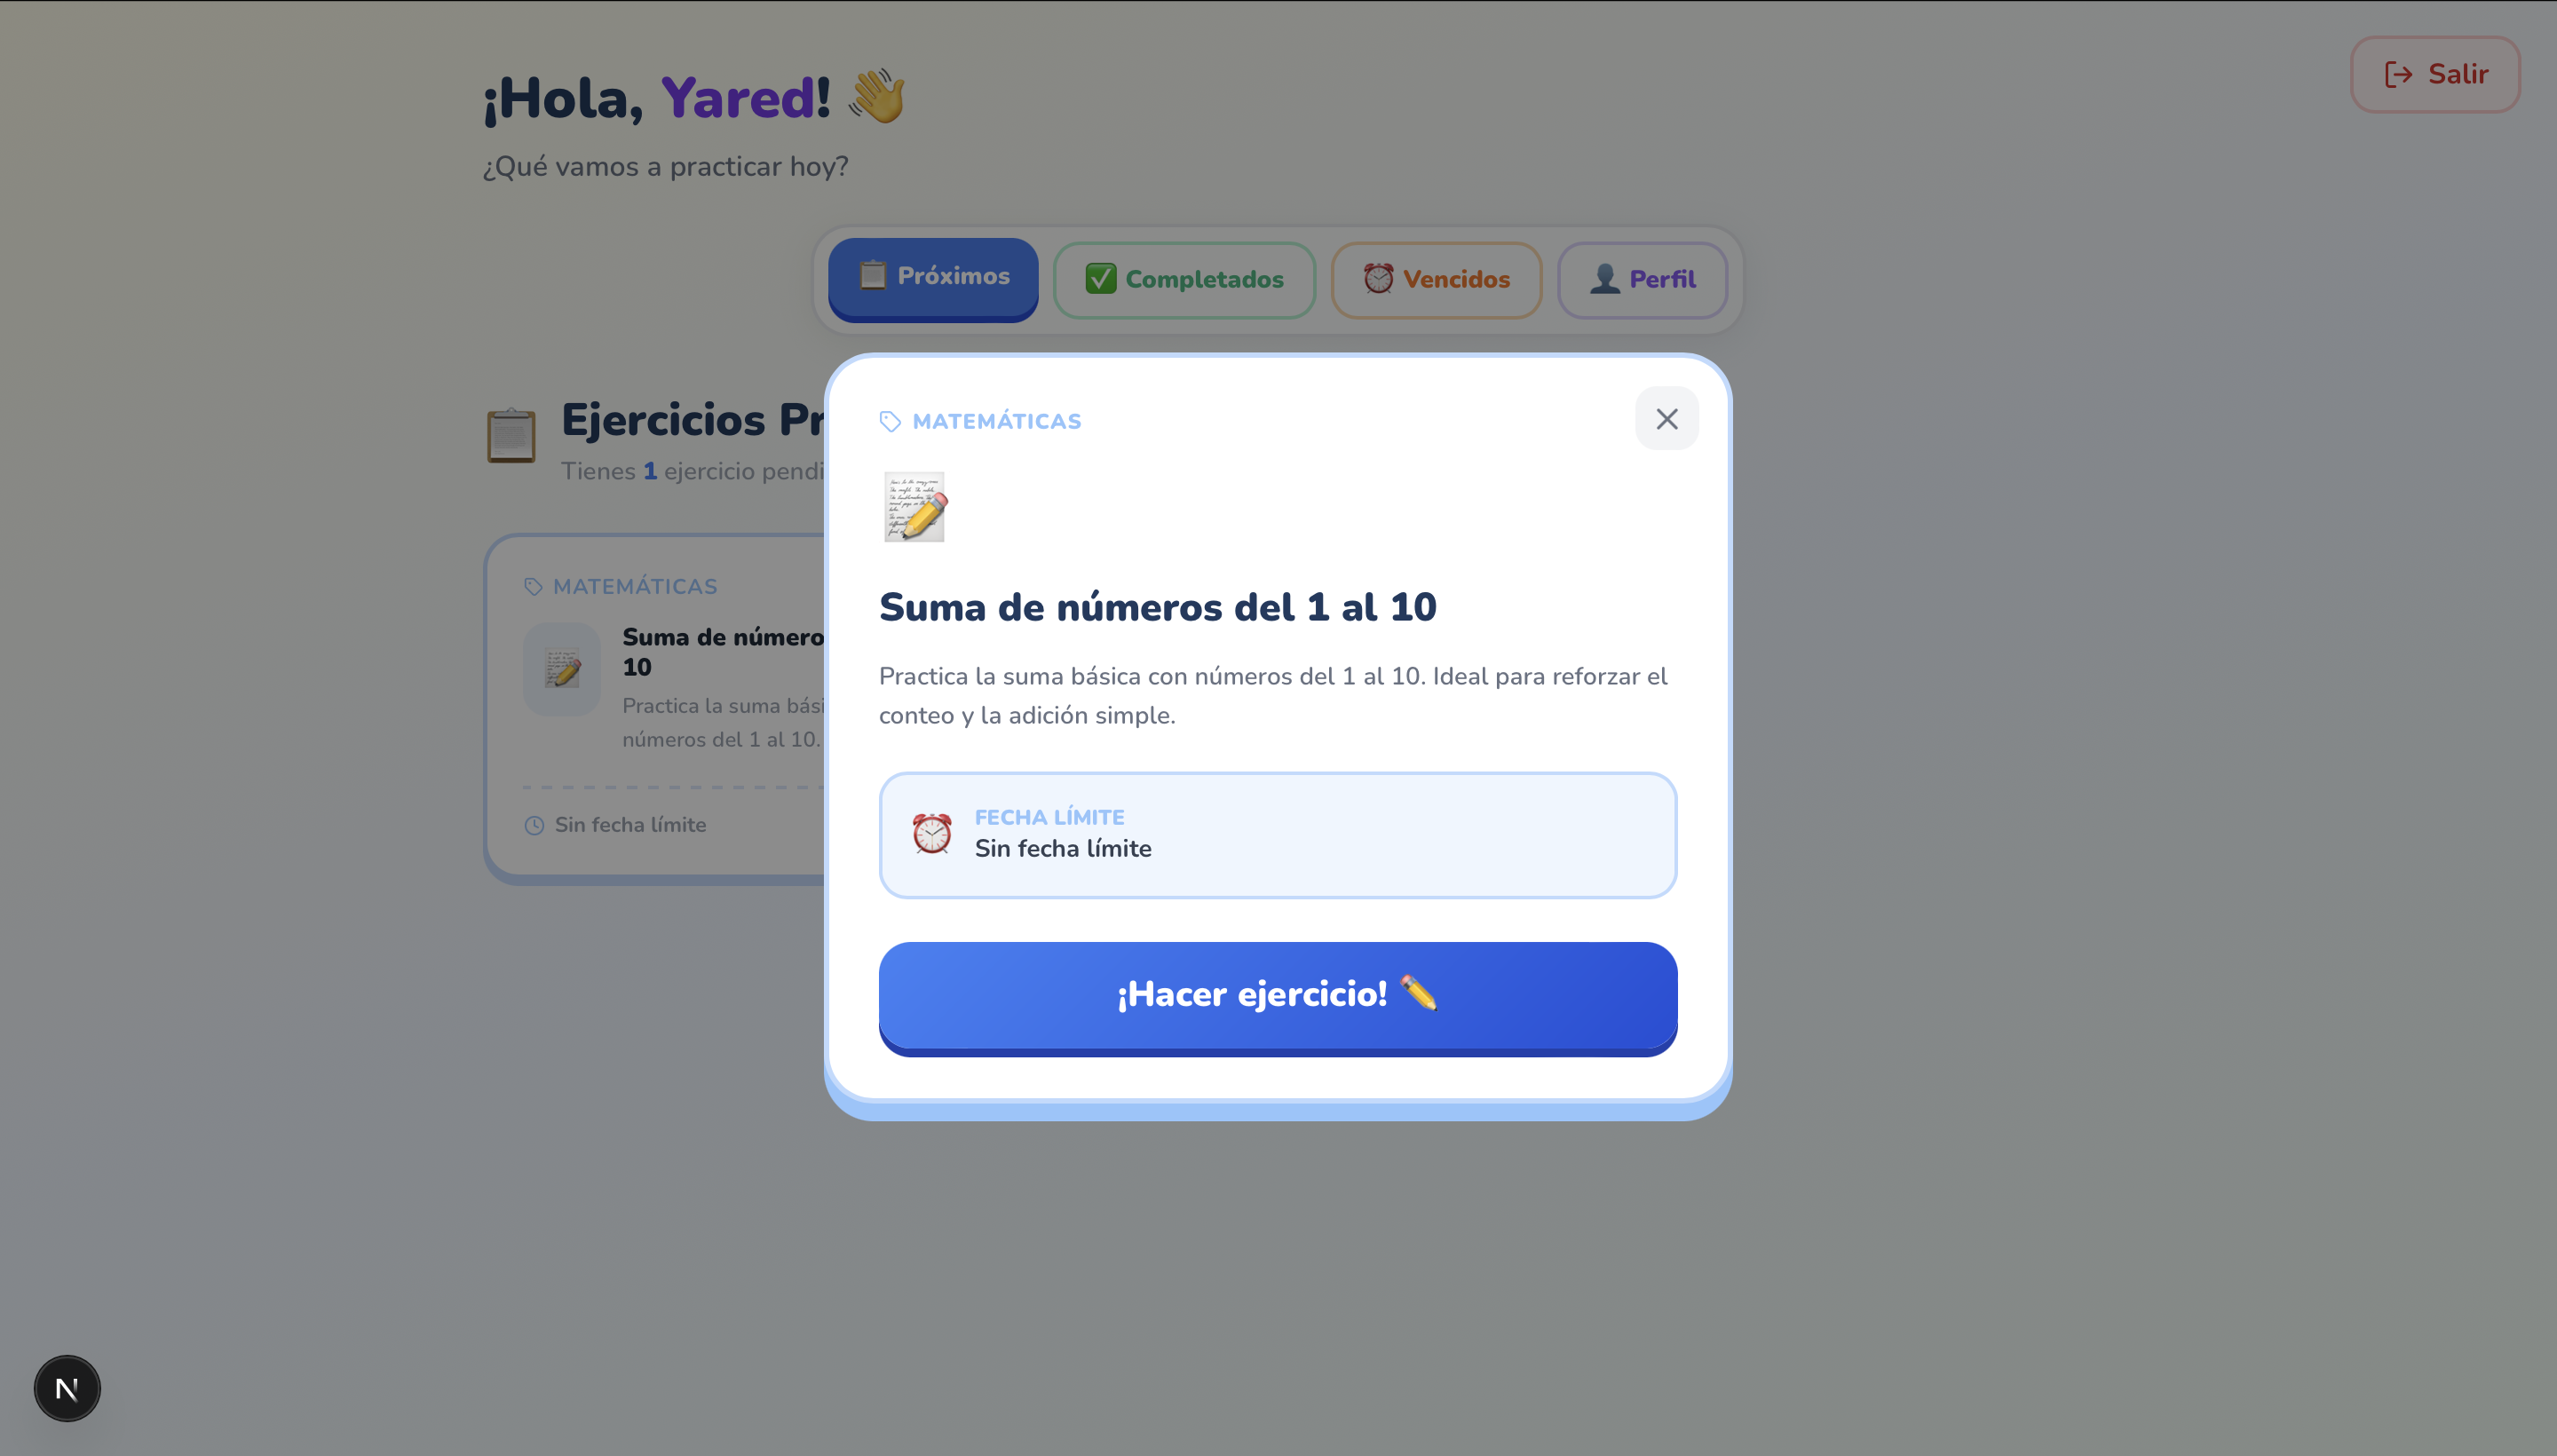
\includegraphics[width=0.7\textwidth]{Imagenes/seleccionEje.png}
    \caption{Visualización de ejercicio a realizar}
    \label{fig:seleccionEje}
\end{figure}

\begin{figure}[H]
    \centering
    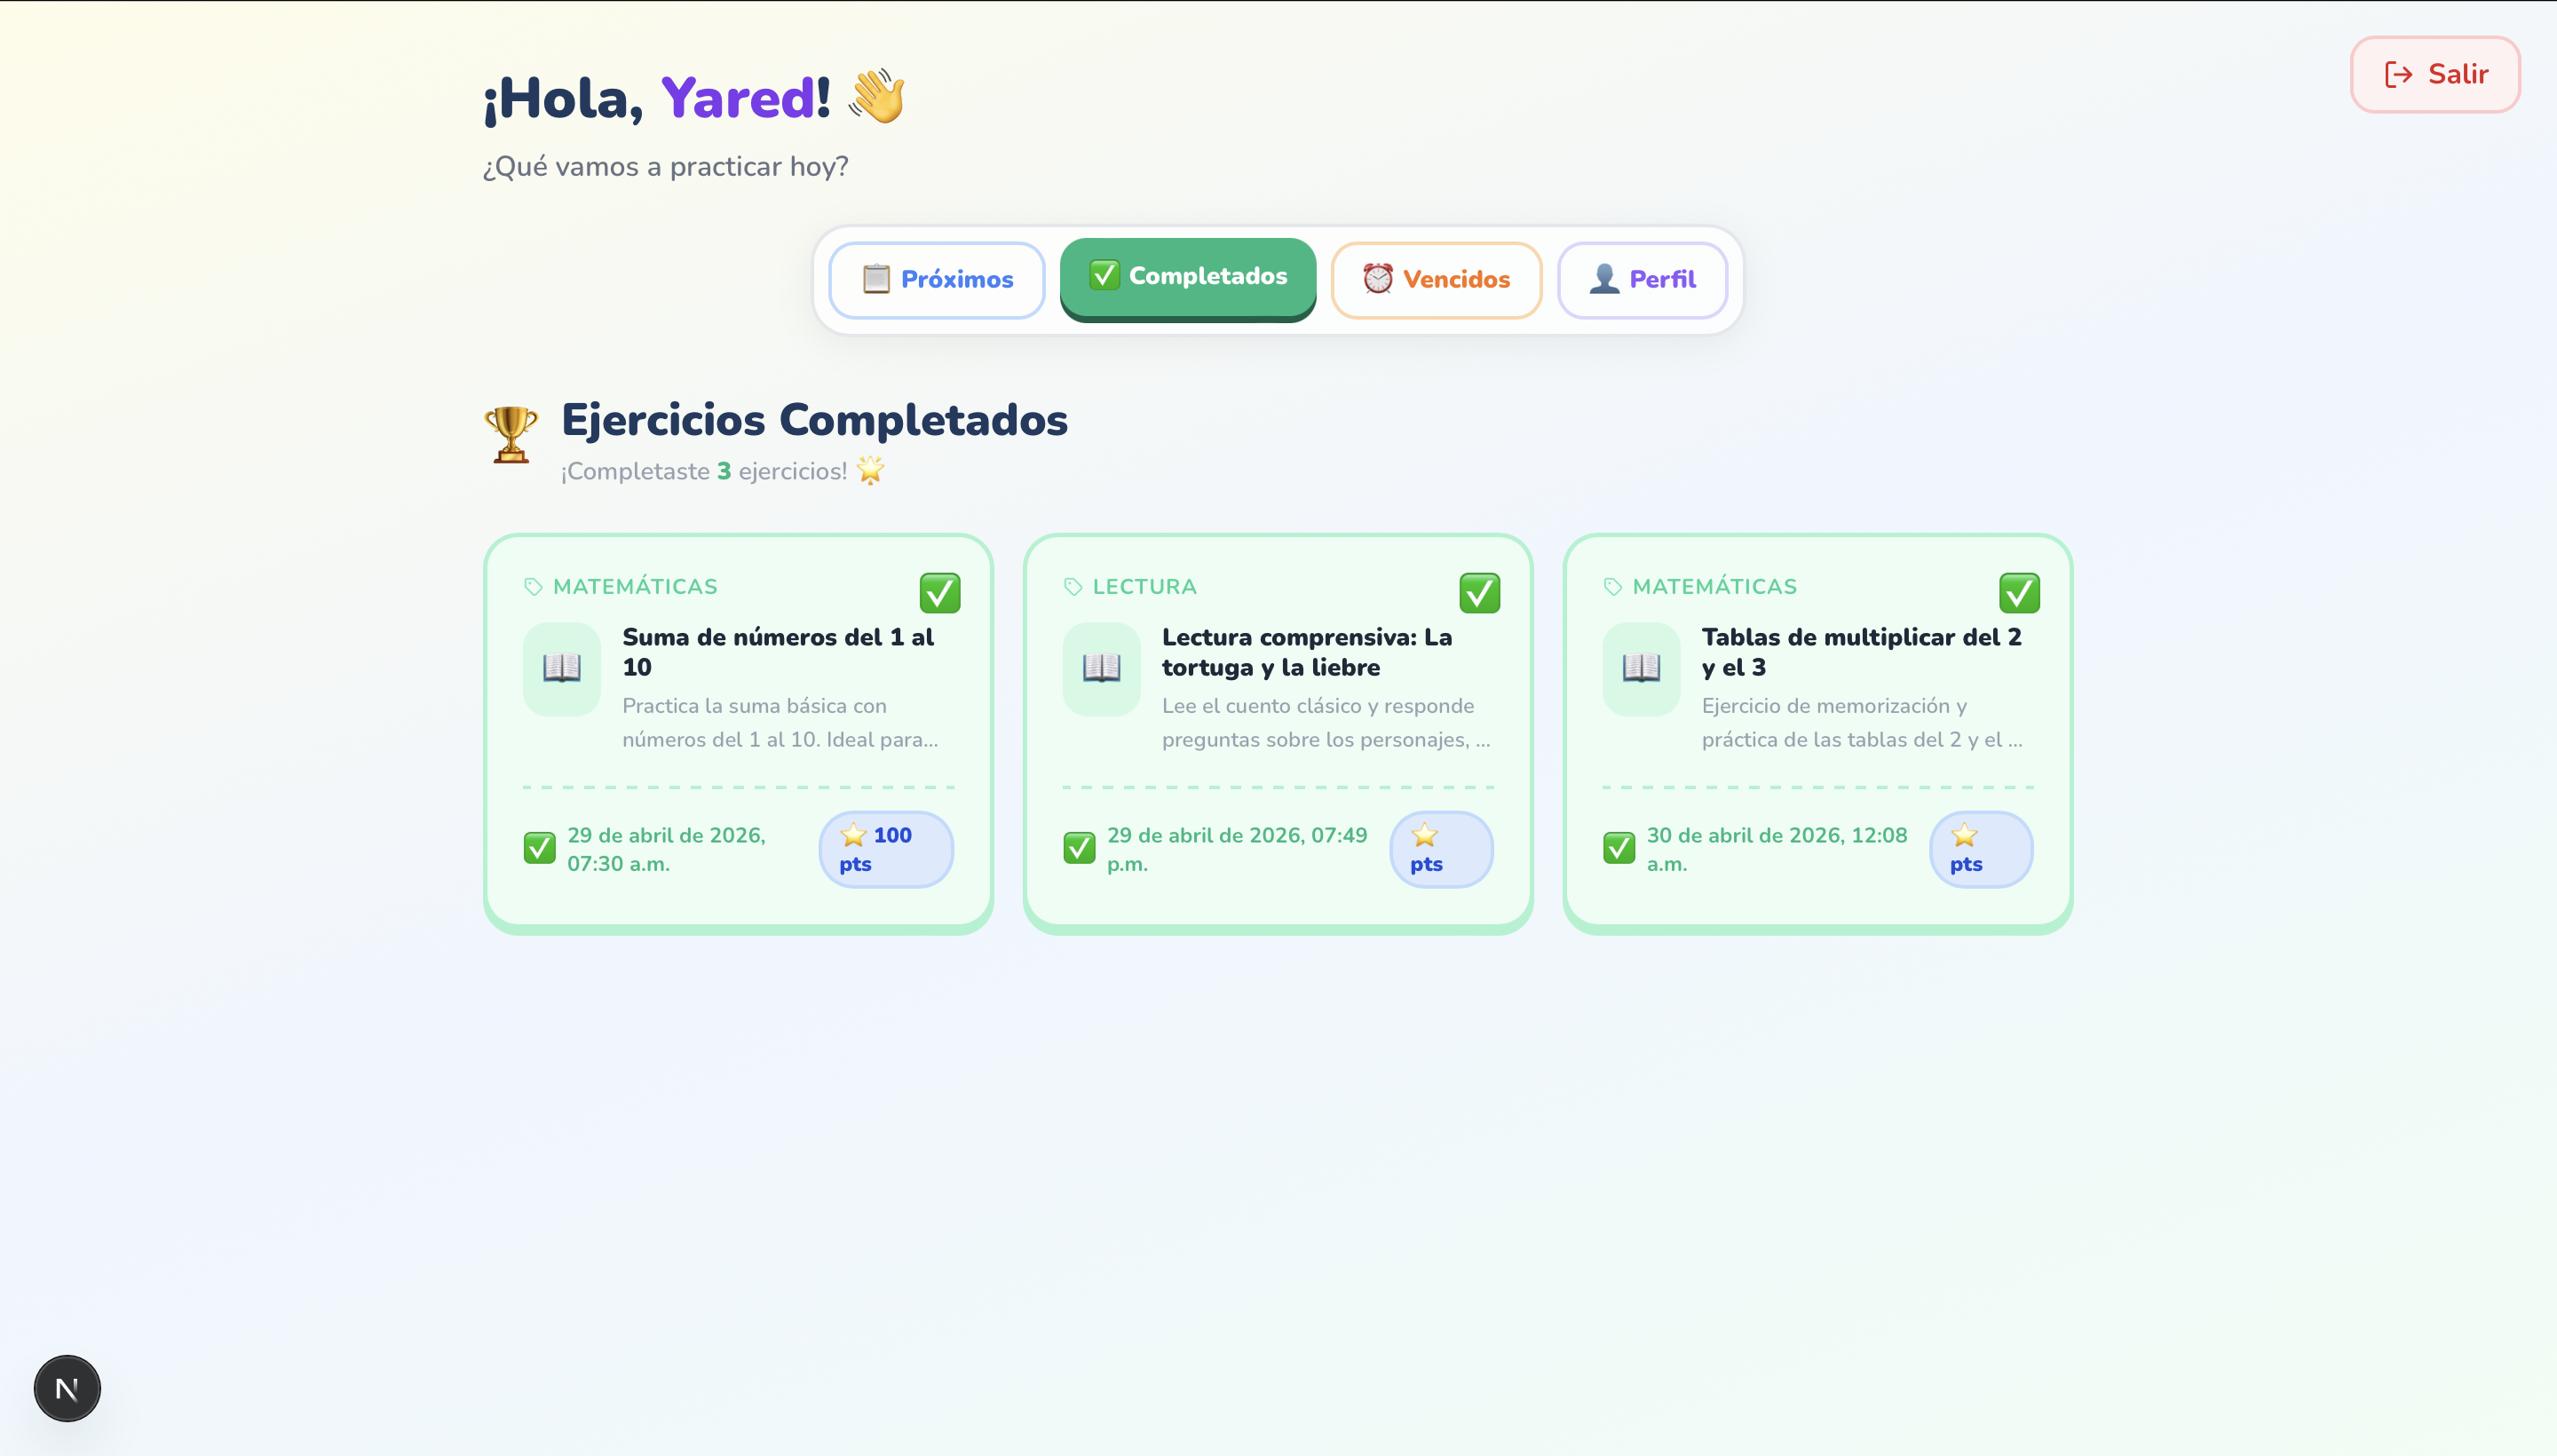
\includegraphics[width=0.7\textwidth]{Imagenes/ejerciciosCompletados.png}
    \caption{Visualización de ejercicios completados por el alumno}
    \label{fig:ejerciciosCompletados}
\end{figure}


\begin{figure}[H]
    \centering
    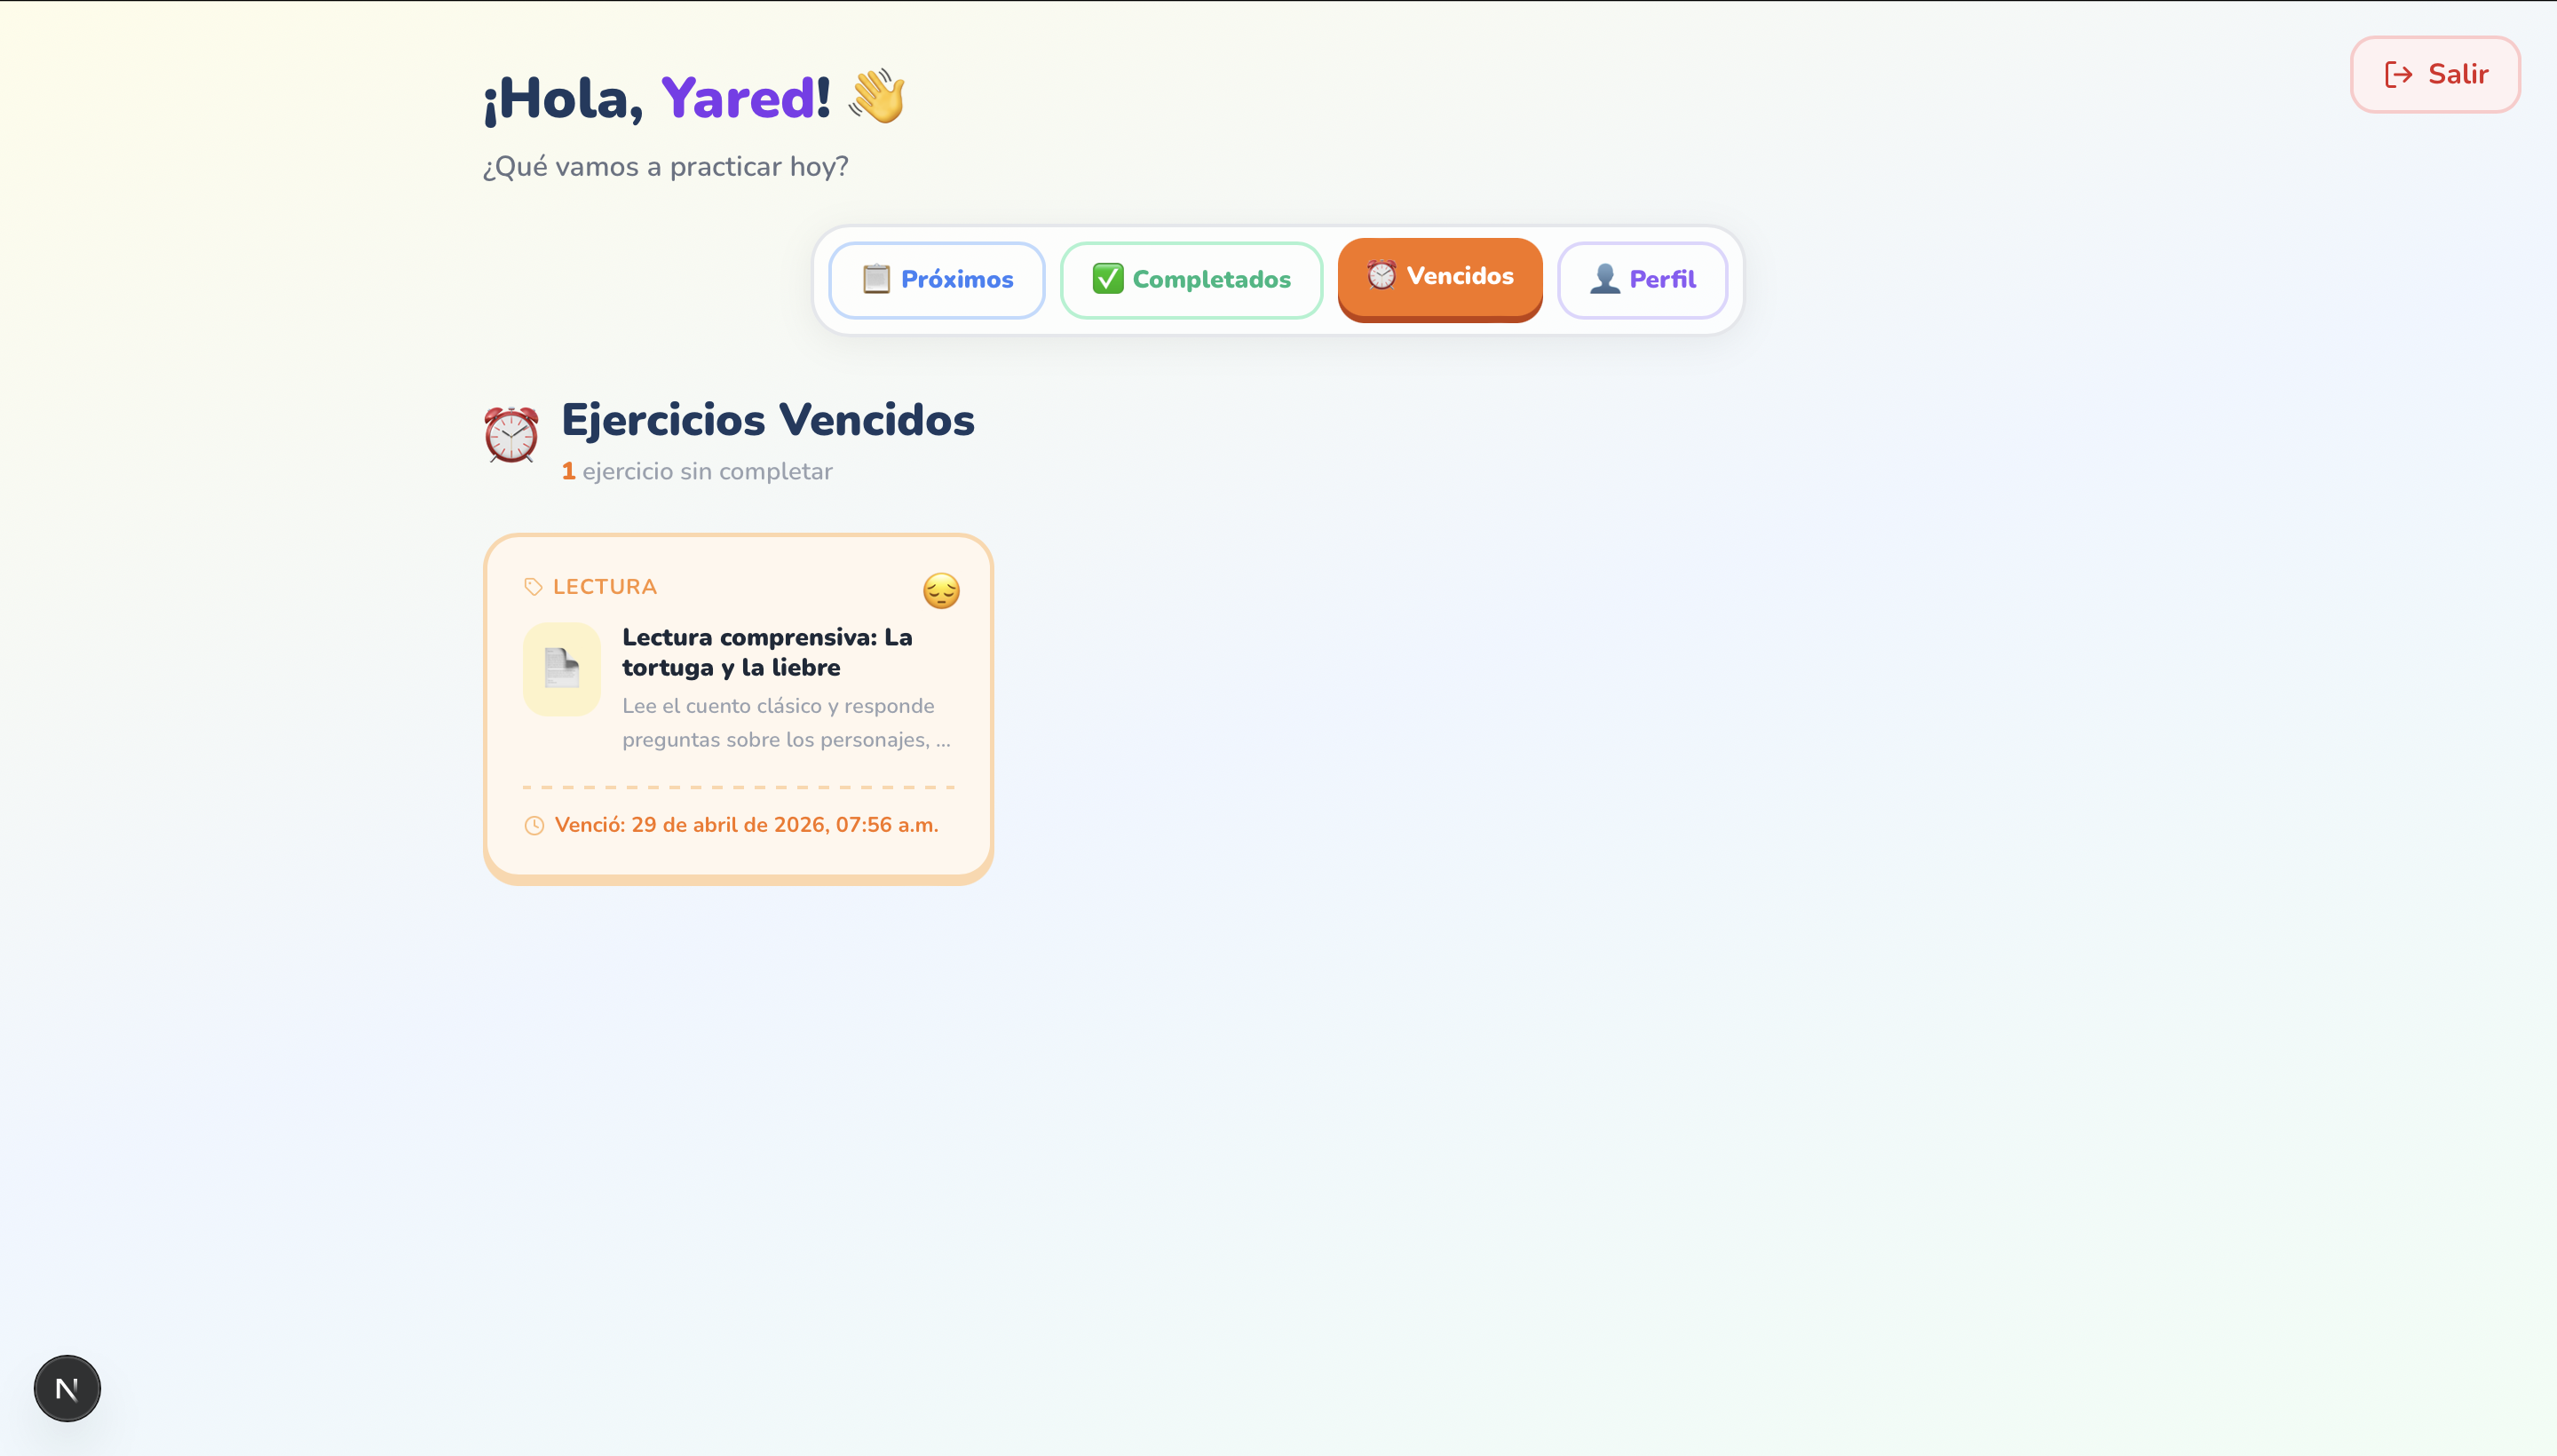
\includegraphics[width=0.7\textwidth]{Imagenes/ejerciciosVencidos.png}
    \caption{Visualización de ejercicios vencidos}
    \label{fig:ejerciciosVencidos}
\end{figure}

\begin{figure}[H]
    \centering
    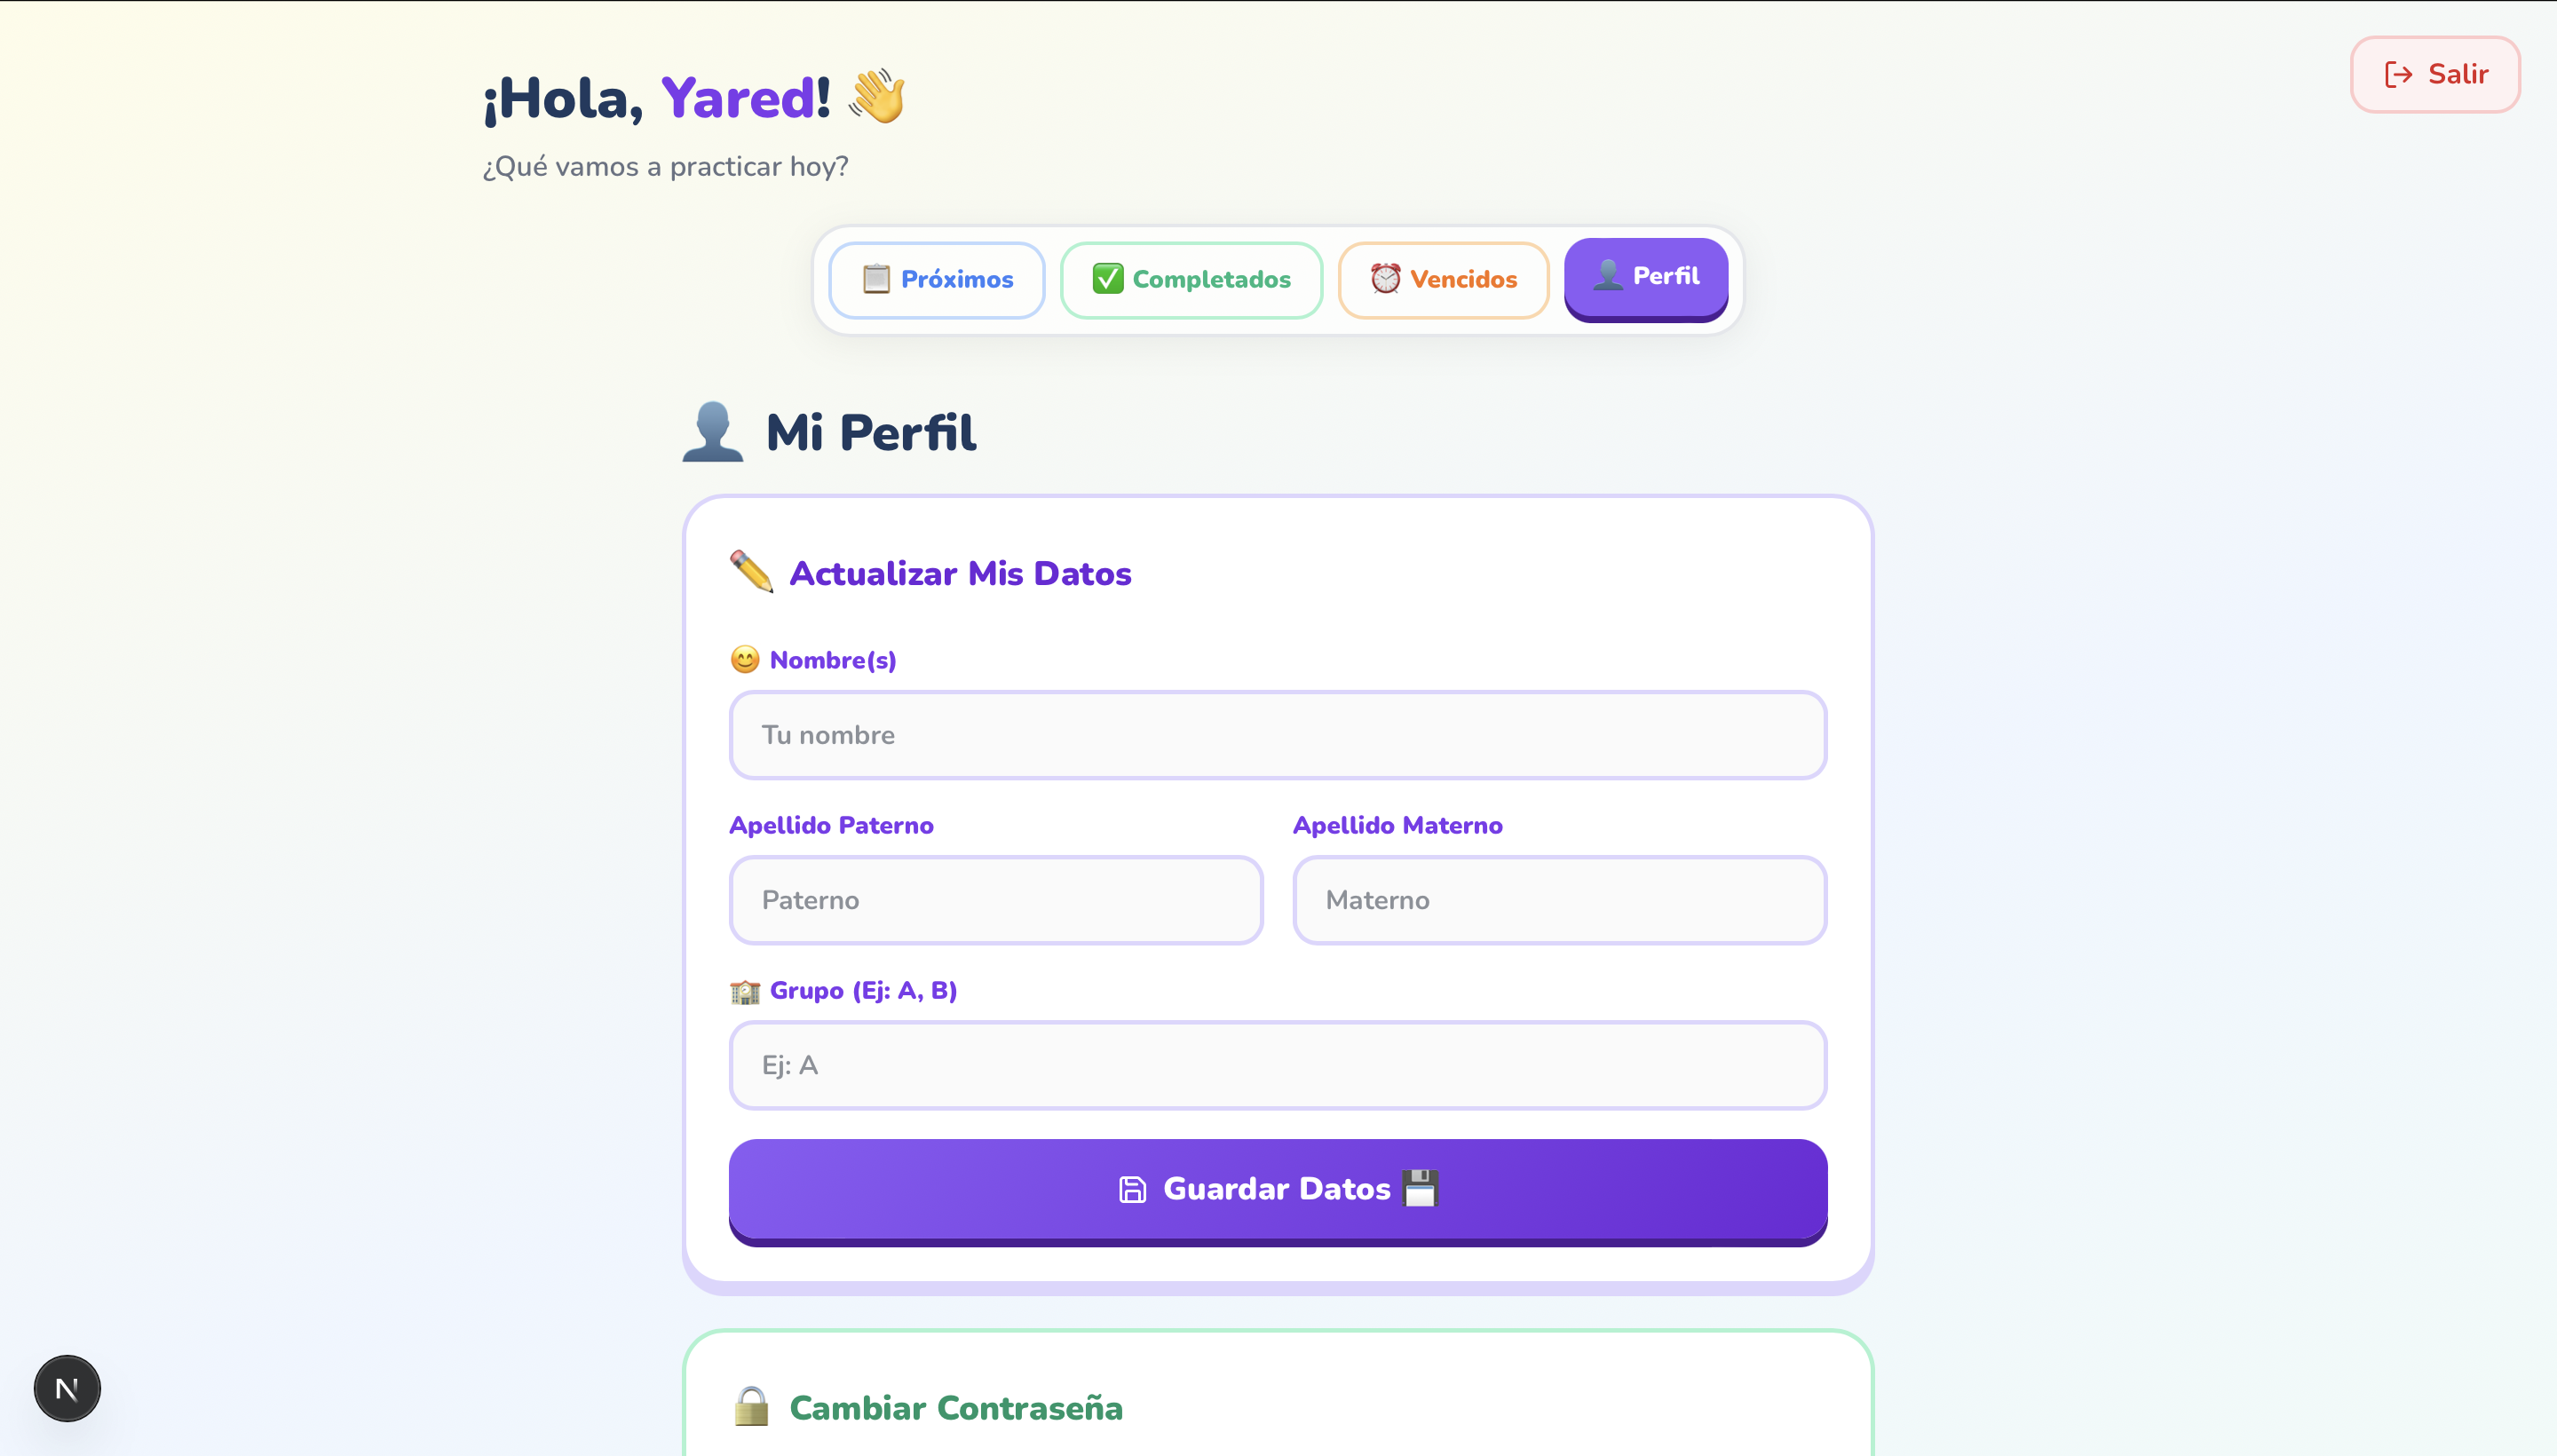
\includegraphics[width=0.7\textwidth]{Imagenes/miperfilA.png}
    \caption{Visualización del perfil del alumno}
    \label{fig:miperfilA}
\end{figure}

\subsubsection{Vista del lienzo digital}

\begin{figure}[H]
    \centering
    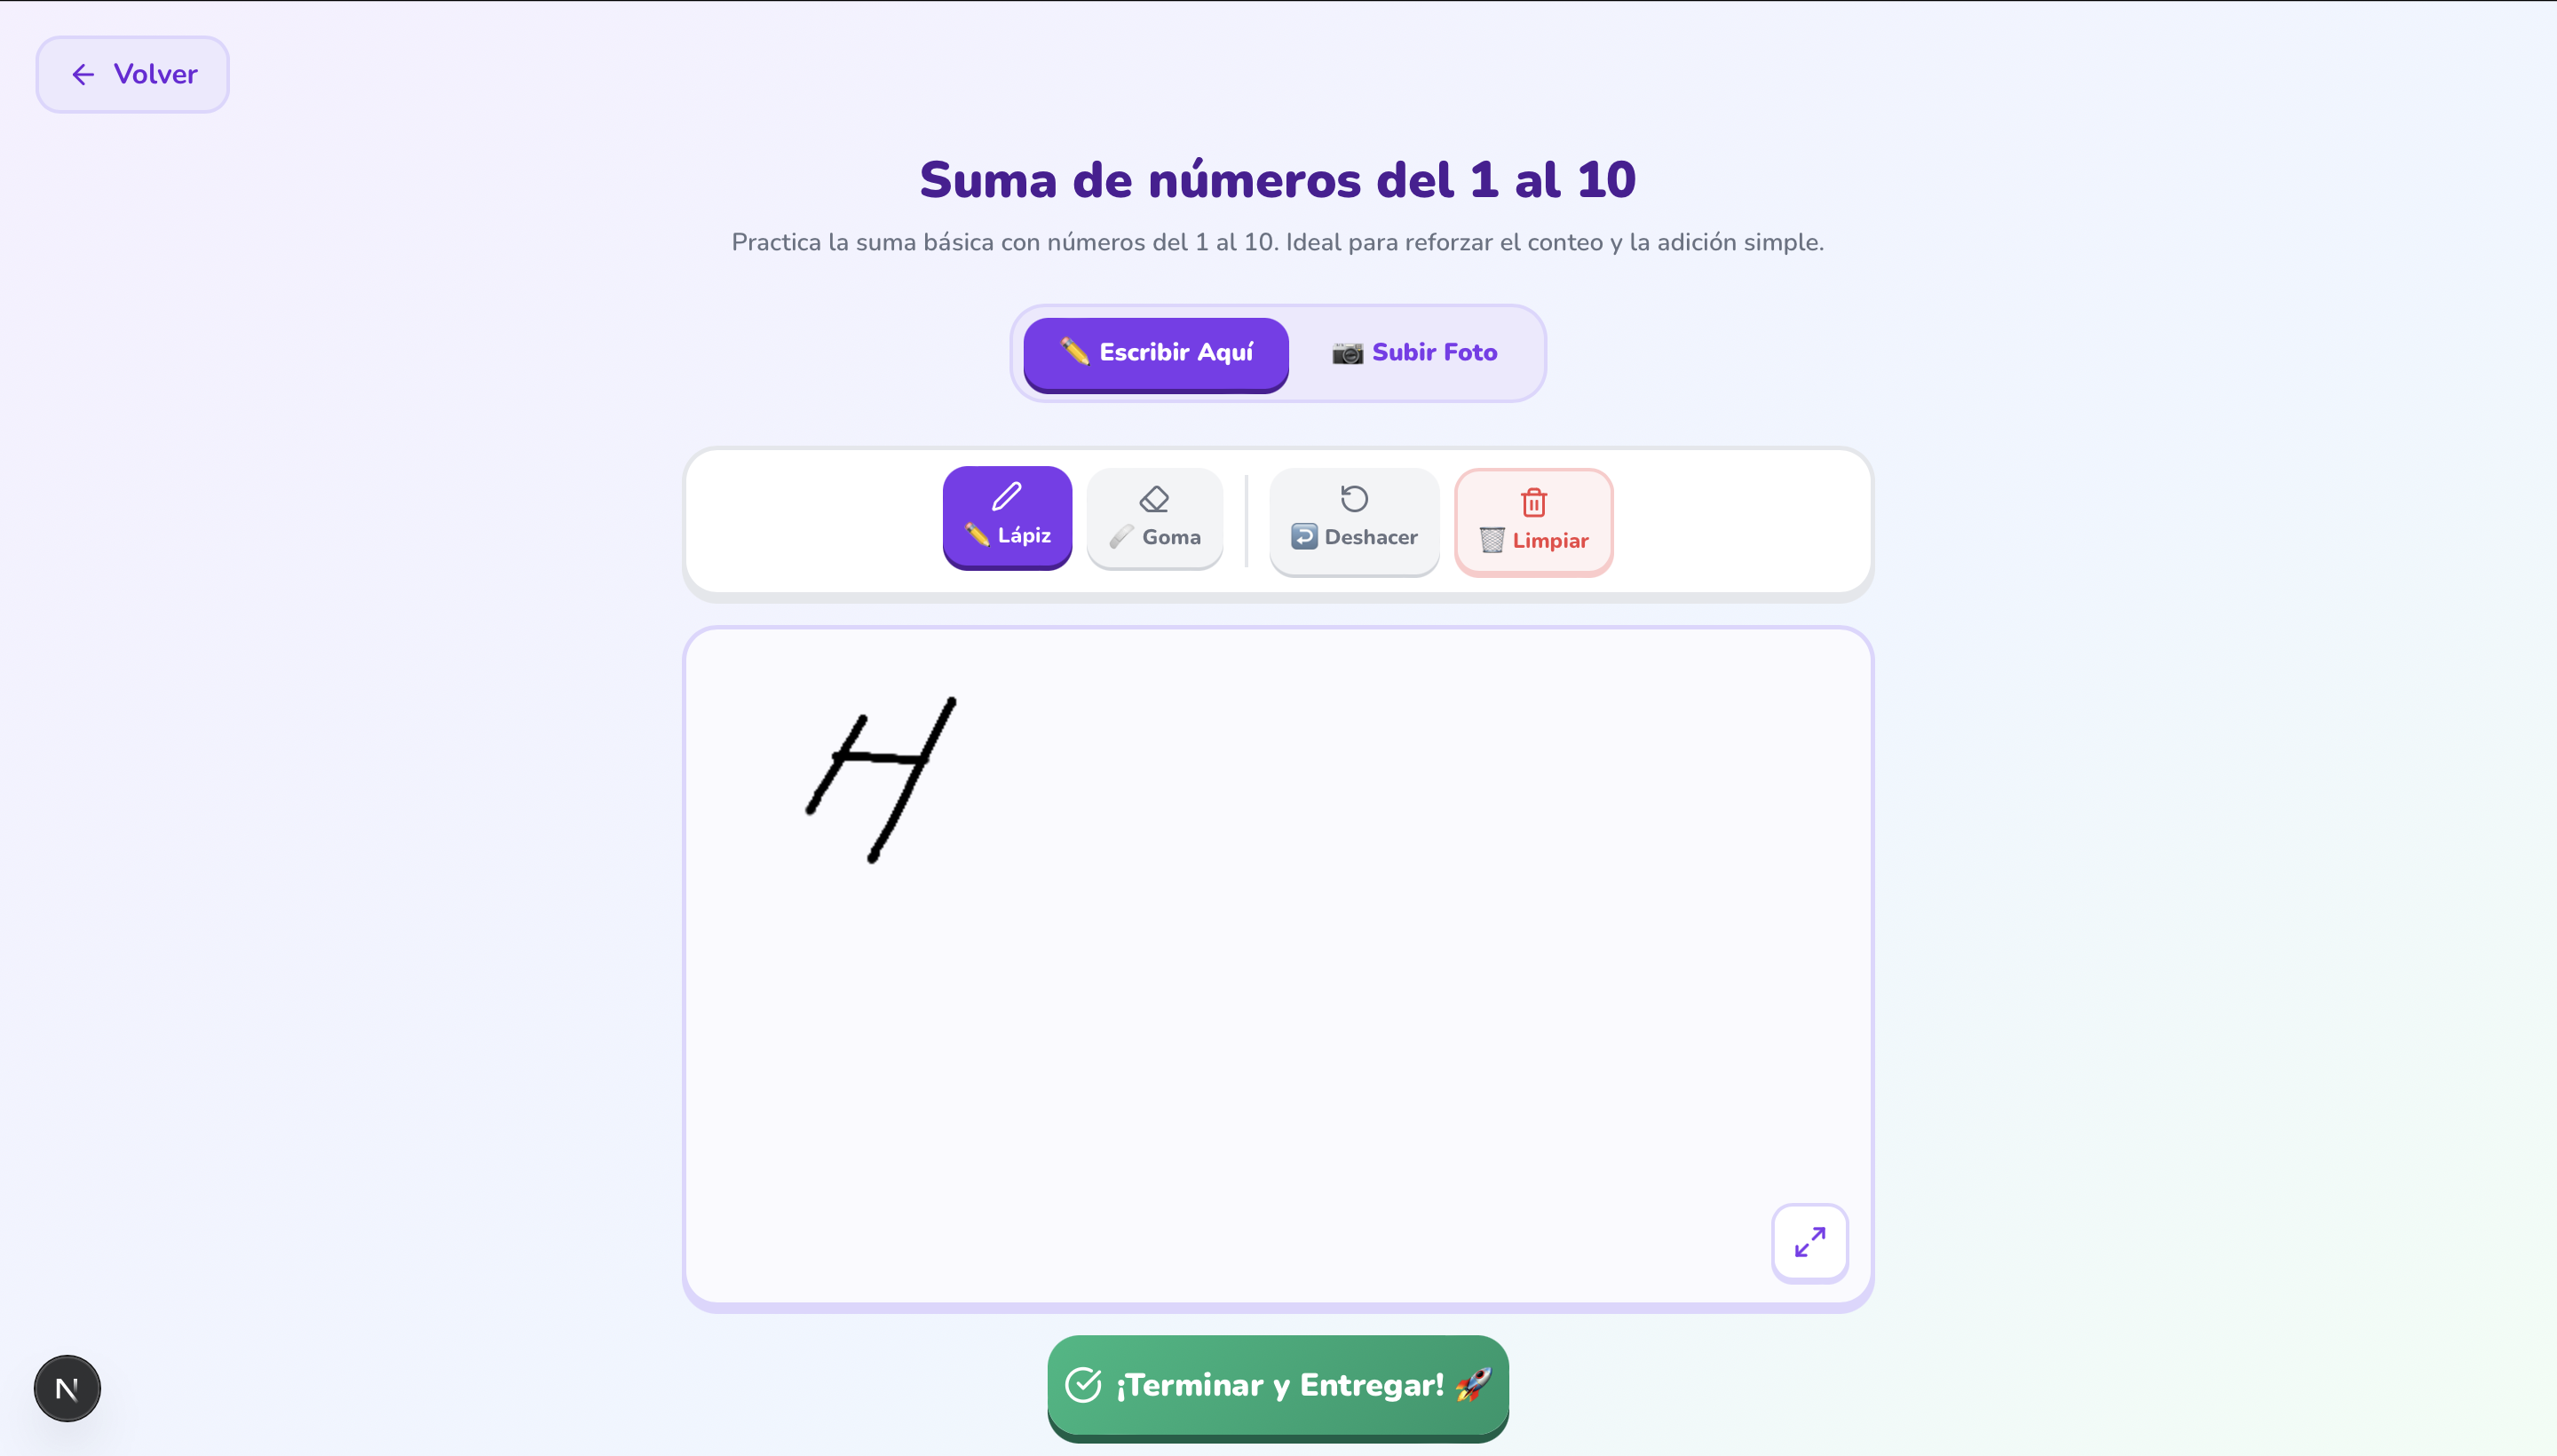
\includegraphics[width=0.7\textwidth]{Imagenes/lienzo.png}
    \caption{Visualización del lienzo digital para realizar ejercicios de escritura}
    \label{fig:lienzo}
\end{figure}


\subsubsection{Vista de captura de escritura}

\begin{figure}[H]
    \centering
    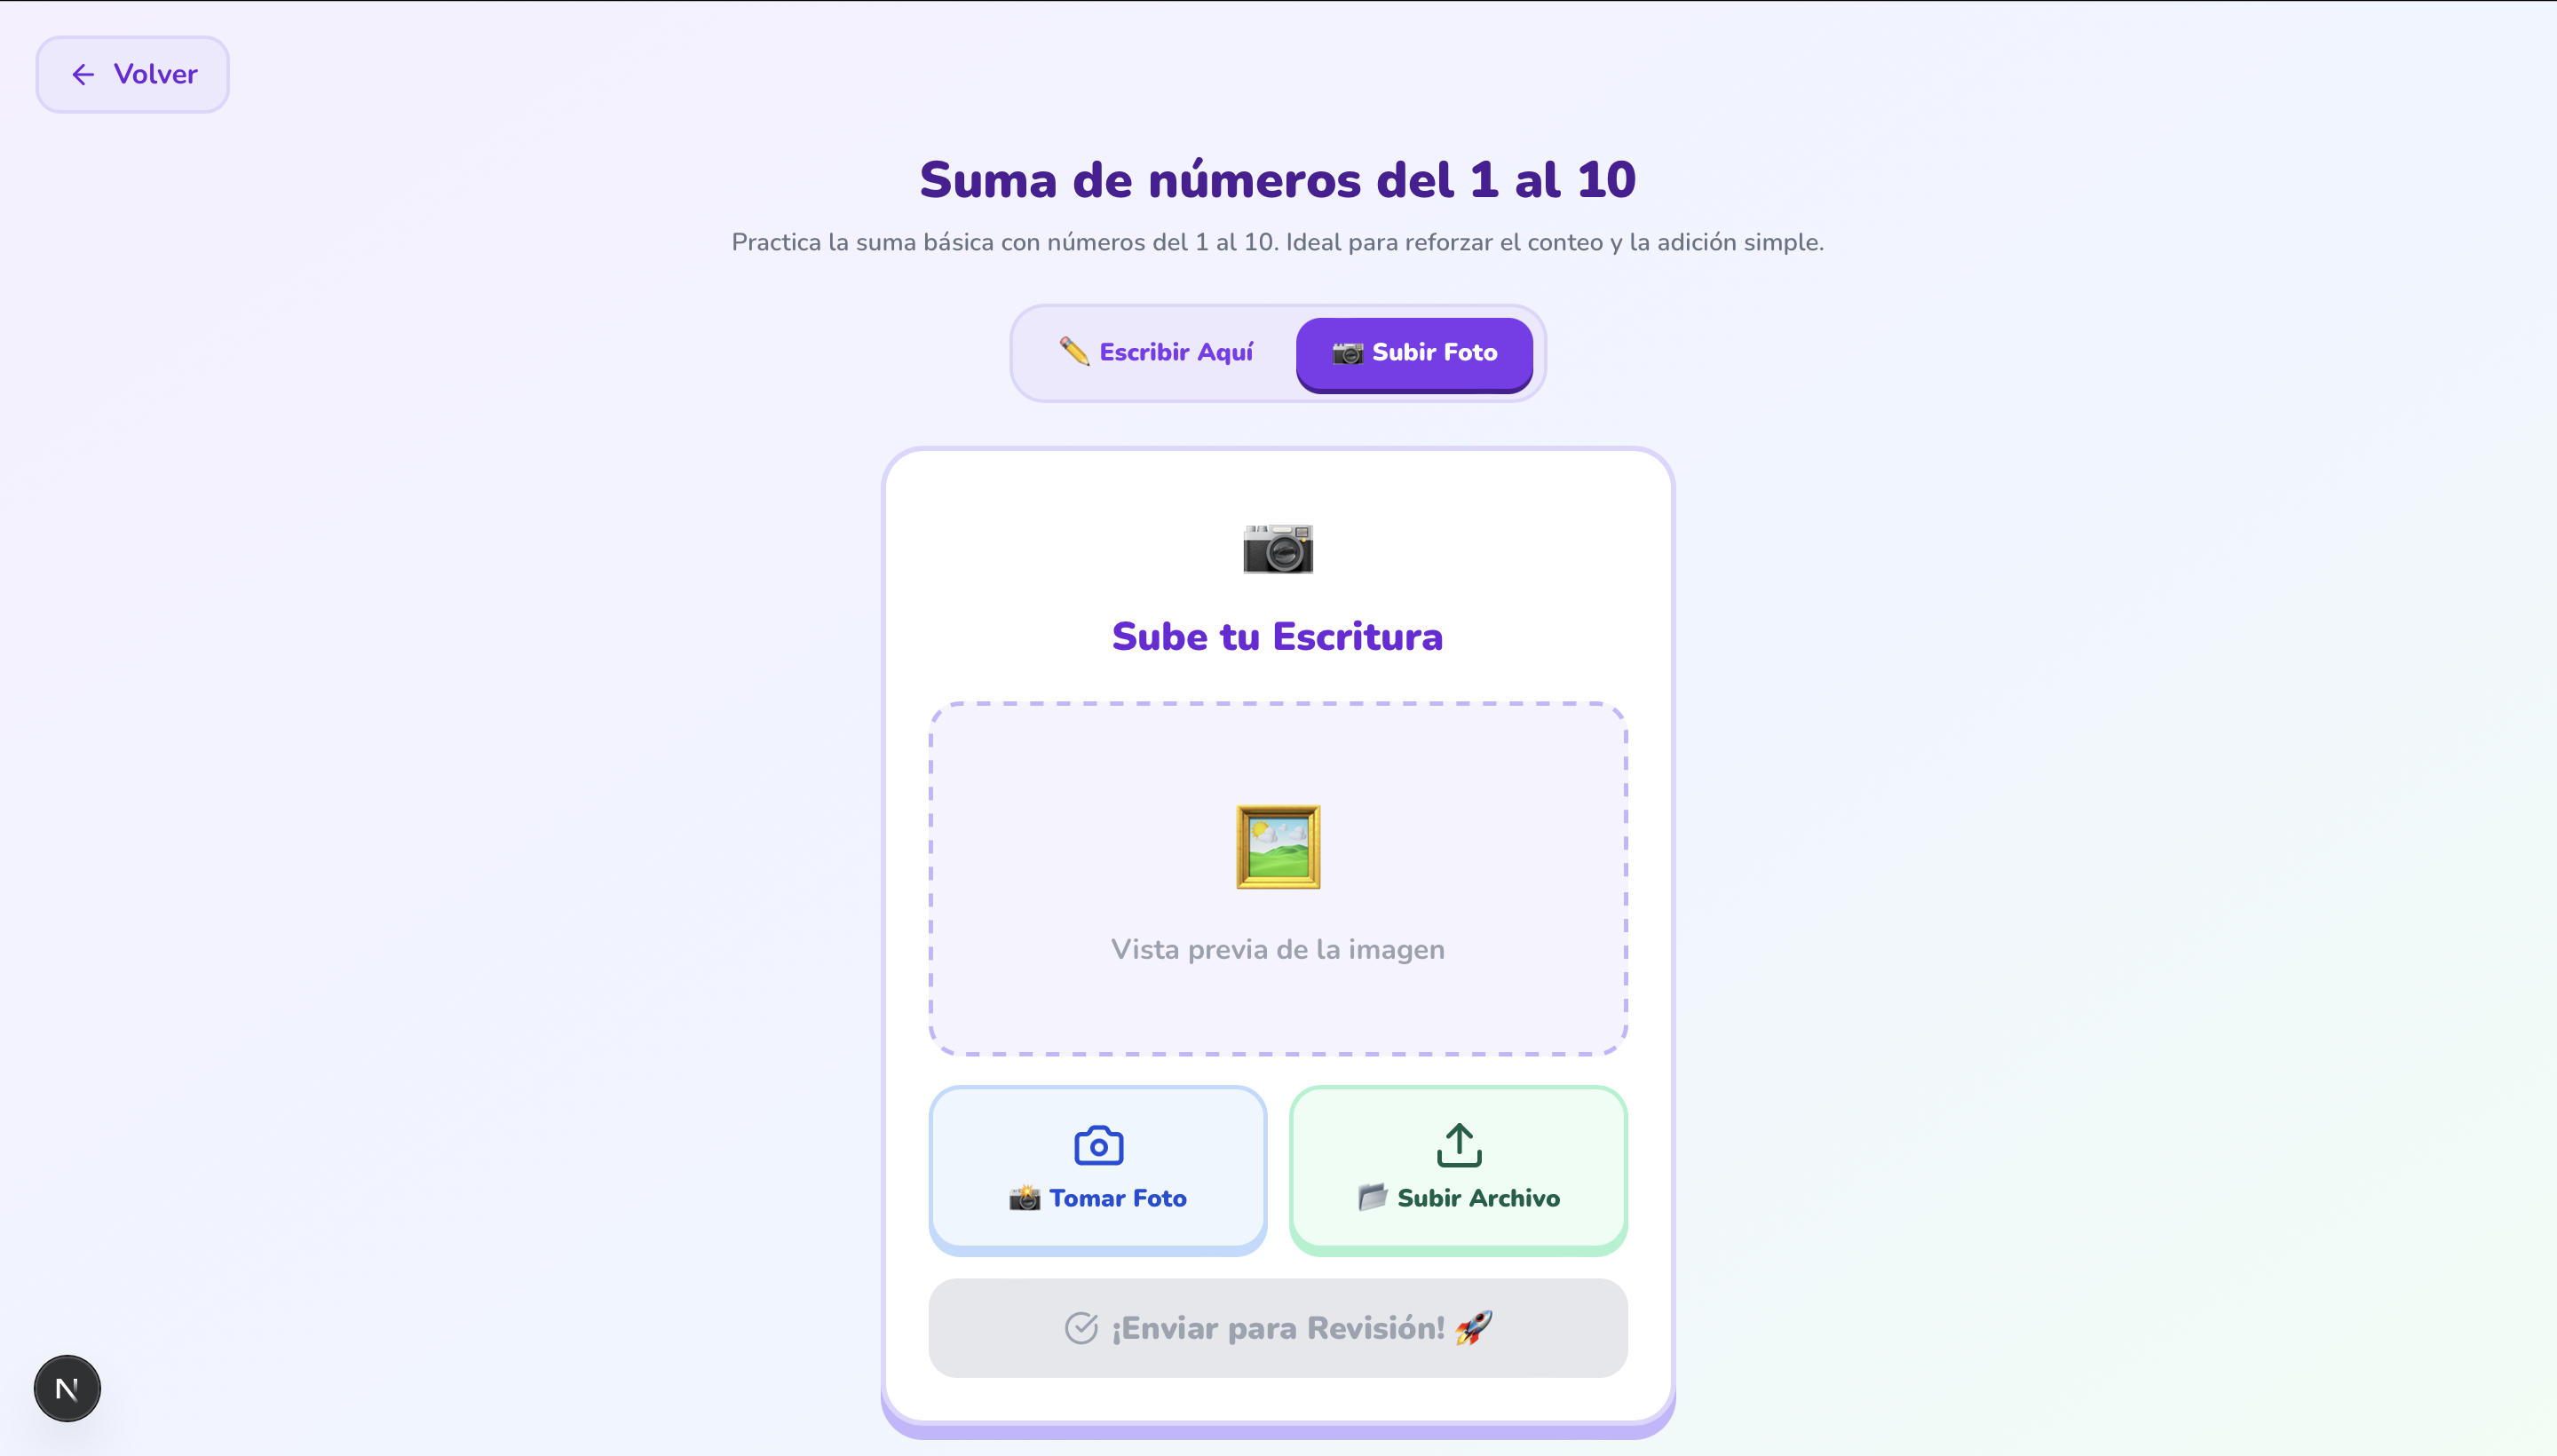
\includegraphics[width=0.7\textwidth]{Imagenes/subirArchivo.png}
    \caption{Visualización de carga de imagen para registrar ejercicios mediante fotografía o archivo}
    \label{fig:subirArchivo}
\end{figure}

\subsubsection{Vista de resultados y retroalimentación}

\begin{figure}[H]
    \centering
    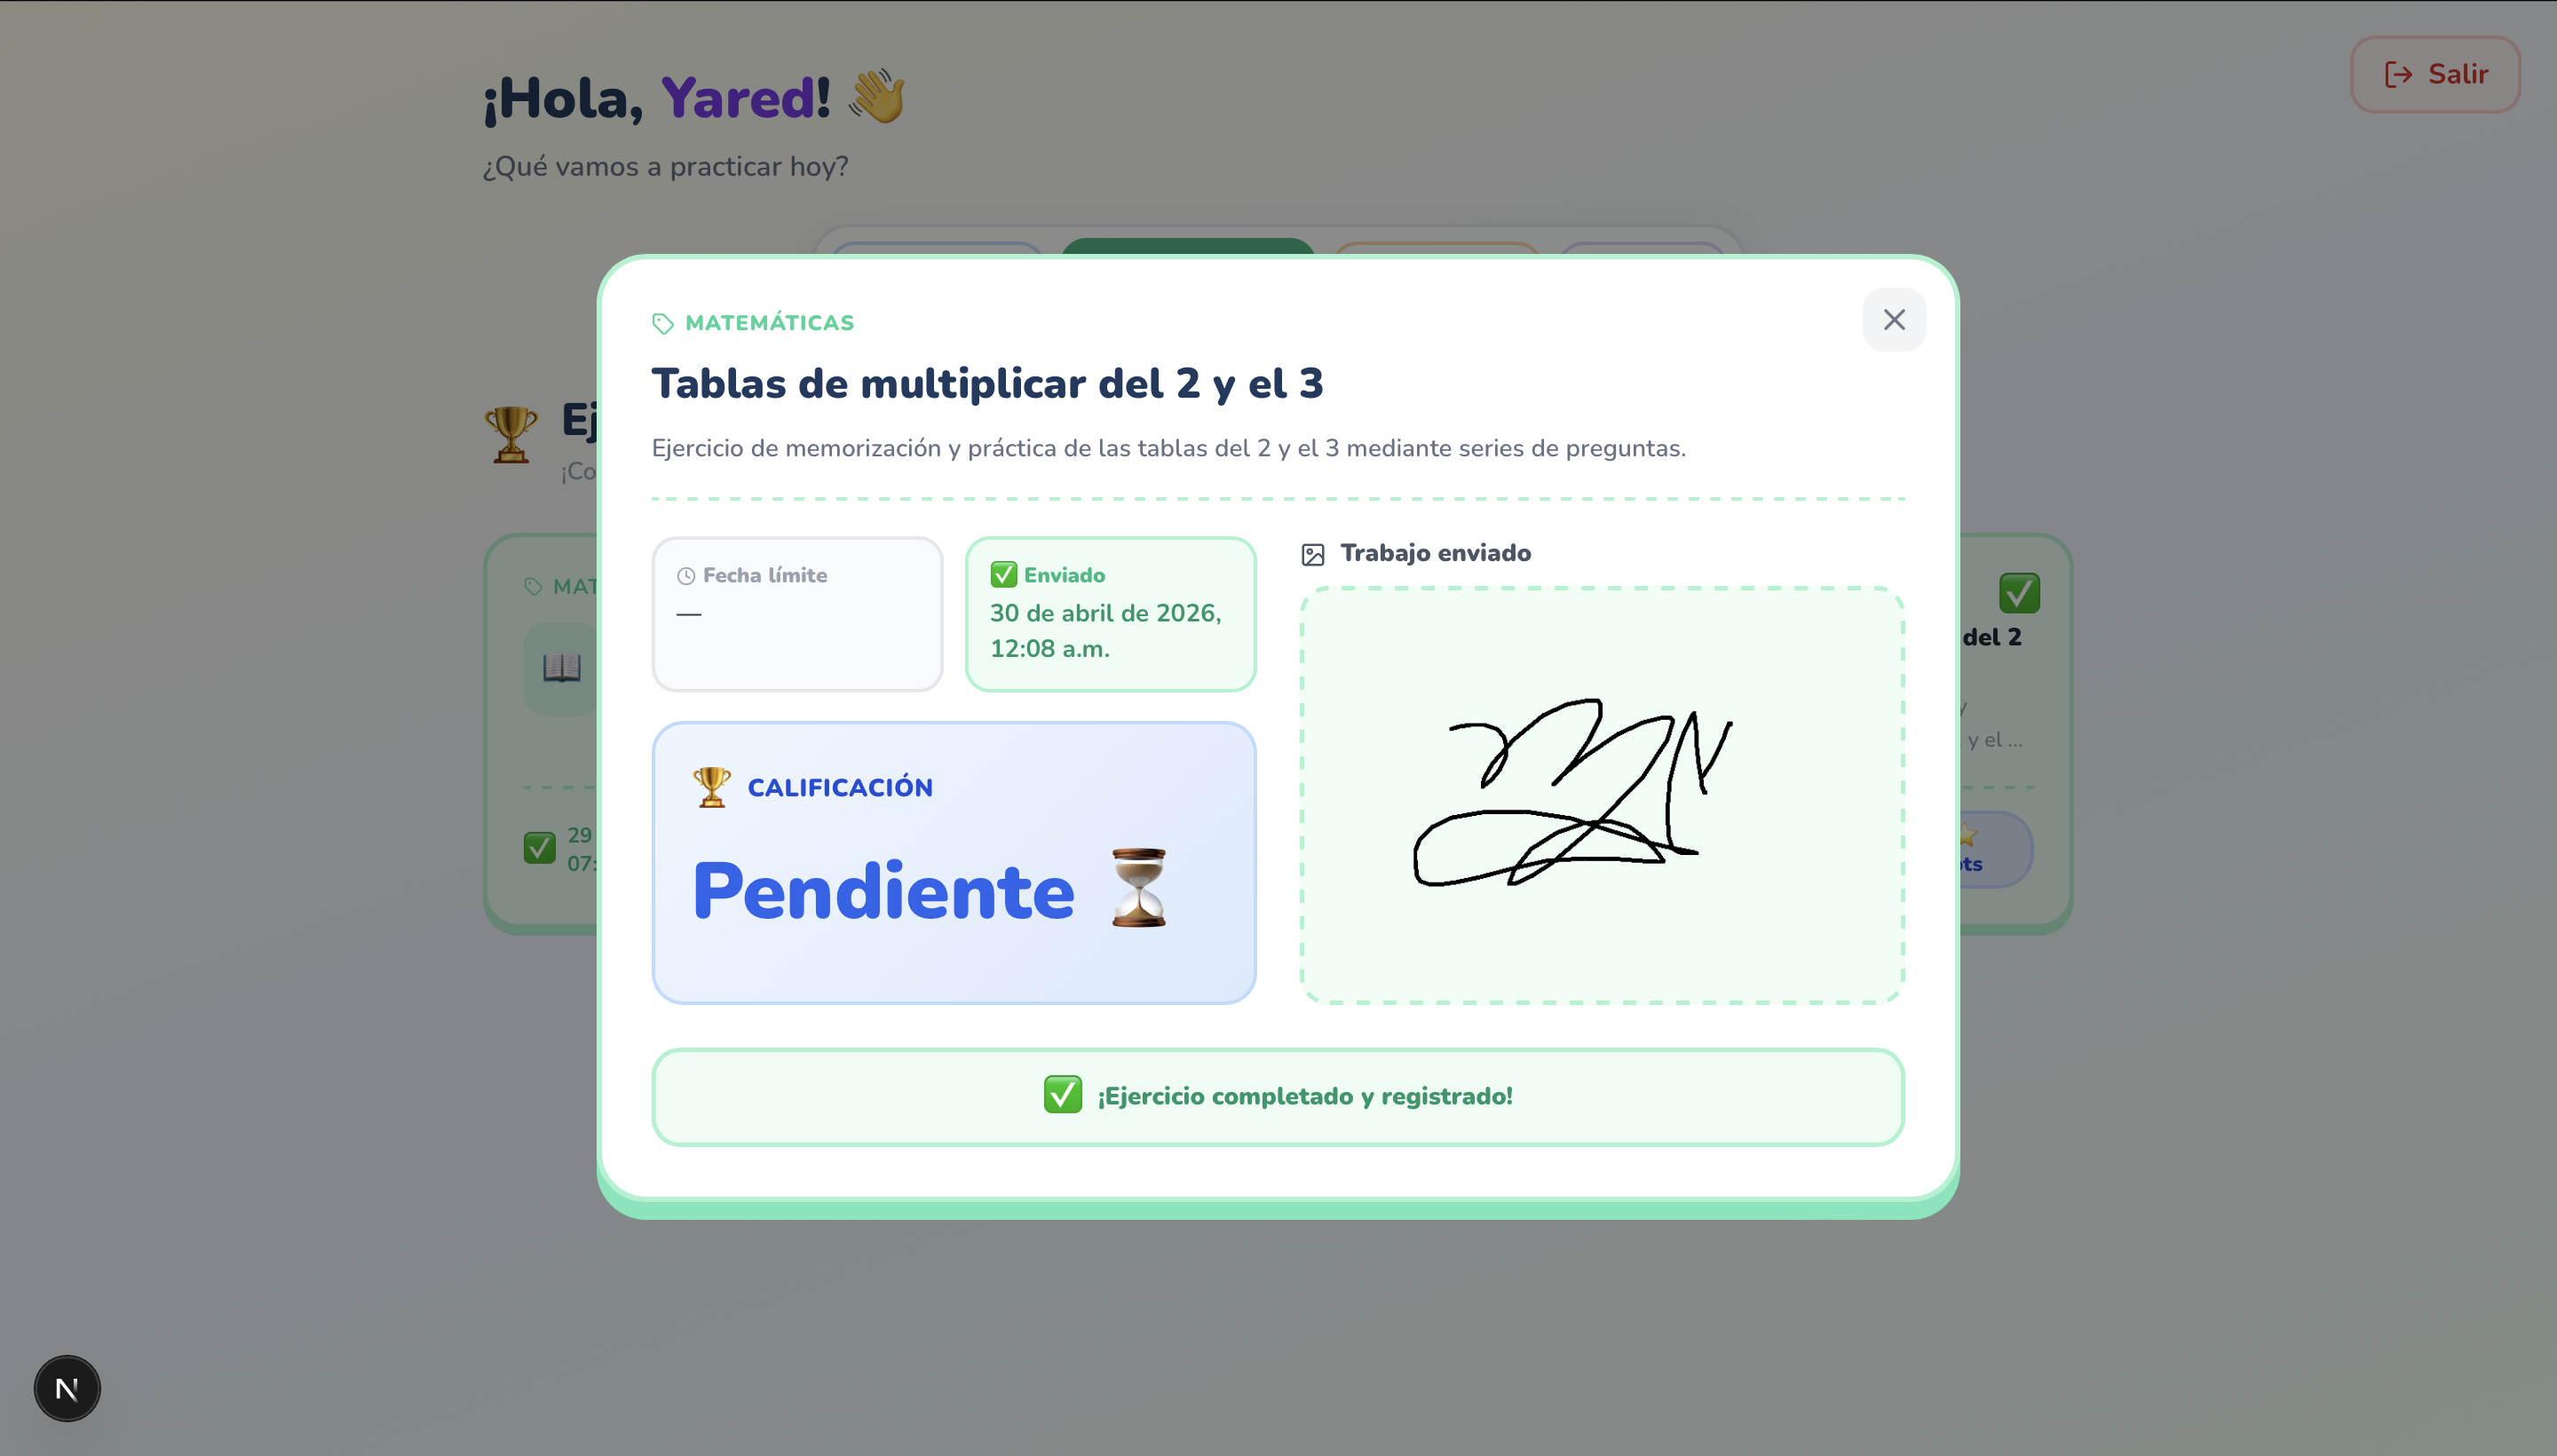
\includegraphics[width=0.7\textwidth]{Imagenes/resultadosEje.png}
    \caption{Visualización de resultados y retroalimentación de ejercicios realizados}
    \label{fig:resultadosEje}
\end{figure}
\section{Capítulo 5: Desarrollo}

En este capítulo se presenta la fase de desarrollo del sistema, en la cual se lleva a cabo la implementación de la arquitectura y el diseño previamente definidos en la etapa de análisis. A partir de los requerimientos funcionales, no funcionales y las reglas de negocio establecidas en el capítulo anterior, se detalla la construcción de los distintos módulos que conforman la plataforma.

\subsection{Desarrollo de la base de datos}

El desarrollo de la base de datos presentado en esta sección se basa en el diagrama relacional y decisiones de diseño de la base de datos. Se llevó a cabo la implementación en el sistema gestor de bases de datos SQL Server, traduciendo cada entidad, atributo y relación en estructuras físicas mediante sentencias T-SQL. 

\subsubsection{Creación del esquema}

Durante esta etapa, se implementaron restricciones de integridad y definición de claves primarias y foráneas, con el objetivo de garantizar la consistencia, eficiencia y correcto funcionamiento de la aplicación web.

\textbf{A. Gestión de usuarios}

Este módulo está compuesto por las tablas \texttt{Usuarios}, \texttt{Tutor} y \texttt{Alumno}, las cuales representan la estructura principal de acceso y perfiles del sistema. La tabla \texttt{Estatus} actúa como catálogo compartido y debe crearse previamente, ya que es referenciada por \texttt{Usuarios} mediante una clave foránea.

\begin{lstlisting}[language=SQL, caption={Implementación simplificada de entidades de usuario}]
    CREATE TABLE Usuarios (
        id_usuario INT IDENTITY(1,1) PRIMARY KEY,
        usuario VARCHAR(50) NOT NULL UNIQUE,
        contrasena_cifrada VARCHAR(255) NOT NULL,
        tipo_usuario VARCHAR(30) NOT NULL,
        id_estatus INT NOT NULL,
        FOREIGN KEY (id_estatus)
            REFERENCES Estatus(id_estatus)
    );
    
    CREATE TABLE Alumno (
        id_alumno INT IDENTITY(1,1) PRIMARY KEY,
        grado VARCHAR(15) NOT NULL,
        grupo VARCHAR(15) NOT NULL,
        id_tutor INT NOT NULL,
        FOREIGN KEY (id_tutor)
            REFERENCES Tutor(id_tutor)
    );
    \end{lstlisting}

\textbf{B. Proceso de evaluación}

Este módulo agrupa las tablas centrales del flujo de evaluación: \texttt{Ejercicio\_Tutor}, \texttt{Intento} y \texttt{Analisis\_ortografico}. La tabla \texttt{Ejercicio\_Tutor} materializa la relación M:N entre tutores y ejercicios del catálogo, incorporando atributos propios de la asignación. La tabla \texttt{Intento} registra cada ejecución de un ejercicio por parte del alumno, almacenando la imagen capturada y el texto reconocido por el módulo OCR. La tabla \texttt{Analisis\_ortografico} almacena los resultados del procesamiento NLP, utilizando un campo JSON para representar las sugerencias de corrección de forma flexible.

\begin{lstlisting}[language=SQL, caption={Estructura simplificada del proceso de evaluación}]
    CREATE TABLE Ejercicio_Tutor (
        id_ejercicio_tutor INT IDENTITY(1,1) PRIMARY KEY,
        id_tutor INT NOT NULL,
        id_ejercicio INT NOT NULL,
        fecha_limite DATETIME NULL,
        id_estatus INT NOT NULL
    );
    
    CREATE TABLE Intentos (
        id_intento INT IDENTITY(1,1) PRIMARY KEY,
        id_alumno INT NOT NULL,
        id_ejercicio_tutor INT NOT NULL,
        texto_detectado_ocr VARCHAR(MAX),
        fecha_envio DATETIME2 DEFAULT GETDATE()
    );
\end{lstlisting}

\subsubsection{Implementación de restricciones e integridad referencial}

Con el objetivo de garantizar la consistencia y calidad de los datos almacenados en la aplicación web, se definieron restricciones de integridad a nivel de base de datos. Estas restricciones operan de forma independiente a la lógica del backend, asegurando que ninguna operación pueda comprometer la coherencia del modelo de datos.

A continuación se describen las restricciones implementadas agrupadas por categoría.

\paragraph{Unicidad de campos críticos}

Se establecieron restricciones \texttt{UNIQUE} en los campos que deben identificar de forma exclusiva a cada registro dentro del sistema, evitando duplicados que comprometan la integridad de la información.

\begin{lstlisting}[
    language=SQL,
    caption={Restricciones de unicidad en campos críticos},
    label={lst:restricciones_unicidad}
]
CONSTRAINT UQ_Usuarios_usuario 
    UNIQUE (usuario),

CONSTRAINT UQ_Tutor_correo 
    UNIQUE (correo),

CREATE UNIQUE INDEX UQ_Intentos_original
ON Intentos (id_alumno, id_ejercicio_tutor)
WHERE id_recomendacion IS NULL;

CREATE UNIQUE INDEX UQ_ET_activo
    ON Ejercicio_Tutor (id_tutor, id_ejercicio)
    WHERE id_estatus = 1;

CONSTRAINT UQ_Analisis_Ort_intento 
    UNIQUE (id_intento),

CONSTRAINT UQ_Analisis_Cal_intento 
    UNIQUE (id_intento)
\end{lstlisting}

\paragraph{Validación de rangos en scores}

Los atributos de puntuación en las tablas \texttt{Analisis\_Ortografico} y \texttt{Analisis\_Caligrafico} deben estar acotados en un rango de 0 a 10, representando la escala de evaluación del sistema. Se implementaron restricciones \texttt{CHECK} para garantizar que ningún valor fuera de este rango pueda ser insertado o actualizado.

\begin{lstlisting}[language=SQL, caption={Restricciones de rango en atributos de puntuación}]
CONSTRAINT CK_ortografia_score
    CHECK (ortografia_score IS NULL 
        OR (ortografia_score >= 0 AND ortografia_score <= 10)),

CONSTRAINT CK_alineacion_score
    CHECK (alineacion_score IS NULL 
        OR (alineacion_score >= 0 AND alineacion_score <= 10)),

CONSTRAINT CK_tamano_letra_score
    CHECK (tamano_letra_score IS NULL 
        OR (tamano_letra_score >= 0 AND tamano_letra_score <= 10)),

CONSTRAINT CK_espaciado_score
    CHECK (espaciado_score IS NULL 
        OR (espaciado_score >= 0 AND espaciado_score <= 10)),

CONSTRAINT CK_inclinacion_score
    CHECK (inclinacion_score IS NULL 
        OR (inclinacion_score >= 0 AND inclinacion_score <= 10))
\end{lstlisting}

\paragraph{Integridad referencial}

Se definieron claves foráneas en todas las entidades que mantienen relaciones entre sí, garantizando que no puedan existir registros huérfanos en el sistema. La siguiente tabla resume las relaciones de integridad referencial implementadas.

\begin{longtable}{|p{4.5cm}|p{4cm}|p{4cm}|}
\caption{Relaciones de integridad referencial del sistema}
\label{tab:integridad_referencial} \\

\hline
\textbf{Tabla origen} & \textbf{Tabla destino} & \textbf{Cardinalidad} \\
\hline
\endfirsthead

\hline
\textbf{Tabla origen} & \textbf{Tabla destino} & \textbf{Cardinalidad} \\
\hline
\endhead

Usuarios & Estatus & N:1 \\
\hline
Tutor & Usuarios & 1:1 \\
\hline
Alumno & Usuarios & 1:1 \\
\hline
Alumno & Tutor & N:1 \\
\hline
Ejercicio\_Tutor & Tutor & N:1 \\
\hline
Ejercicio\_Tutor & Ejercicio & N:1 \\
\hline
Ejercicio\_Tutor & Estatus & N:1 \\
\hline
Intentos & Alumno & N:1 \\
\hline
Intentos & Ejercicio\_Tutor & N:1 \\
\hline
Analisis\_Ortografico & Intentos & 1:1 \\
\hline
Sugerencia\_ortografica & Analisis\_Ortografico & N:1 \\
\hline
Analisis\_Caligrafico & Intentos & 1:1 \\
\hline

\end{longtable}

\paragraph{Obligatoriedad de campos}

Se establecieron restricciones \texttt{NOT NULL} en todos los atributos que son indispensables para el funcionamiento del sistema, garantizando que ningún registro pueda ser insertado sin la información mínima requerida. Los campos marcados como \texttt{NULL} corresponden a información opcional o generada de forma asíncrona, como el texto detectado por OCR o los scores de análisis, los cuales se completan una vez procesado el intento.

\subsubsection{Implementación de la vista vw\_historial\_alumno}

La vista \texttt{vw\_historial\_alumno} se creó con el objetivo de consolidar en una única consulta predefinida la información distribuida entre las tablas \texttt{Intentos}, \texttt{Analisis\_Ortografico}, \texttt{Analisis\_Caligrafico}, \texttt{Alumno} y \texttt{Ejercicio}. Su implementación responde a tres necesidades concretas del sistema:

\begin{itemize}
    \item \textbf{Rendimiento:} evita la ejecución repetitiva de consultas con múltiples \texttt{JOIN} cada vez que el tutor consulta el historial de un alumno (RF-09) o el alumno revisa sus ejercicios completados (RF-16).
    \item \textbf{Separación de responsabilidades:} el controlador accede al historial mediante una consulta simple sobre la vista, sin necesidad de conocer la estructura interna de las tablas involucradas, lo cual es coherente con el patrón MVC adoptado.
    \item \textbf{Normalización:} permite mantener el modelo de datos normalizado sin sacrificar la facilidad de consulta, ya que la vista actúa como capa de abstracción sobre las relaciones existentes sin almacenar datos redundantes.
\end{itemize}

Se utilizaron \texttt{LEFT JOIN} en las tablas de análisis para contemplar el caso en que un intento recién enviado aún no haya sido procesado por los módulos OCR y NLP, mostrando \texttt{NULL} en los scores mientras el análisis está pendiente.

\begin{lstlisting}[language=SQL, caption={Implementación de la vista vw\_historial\_alumno}]
CREATE VIEW vw_historial_alumno AS
SELECT
    a.id_alumno,
    u.nombre                        AS nombre_alumno,
    e.id_ejercicio,
    e.titulo                        AS titulo_ejercicio,
    e.tipo                          AS tipo_ejercicio,
    i.id_intento,
    i.fecha_envio,
    i.retroalimentacion,
    CASE
        WHEN i.id_recomendacion IS NULL
        THEN 'Original'
        ELSE 'Reintento'
    END                             AS tipo_intento,
    ao.ortografia_score,
    ao.cantidad_errores,
    ac.alineacion_score,
    ac.tamano_letra_score,
    ac.espaciado_score,
    ac.inclinacion_score
FROM Intentos i
INNER JOIN Alumno a
    ON a.id_alumno = i.id_alumno
INNER JOIN Usuarios u
    ON u.id_usuario = a.id_usuario
INNER JOIN Ejercicios_Tutor et
    ON et.id_ejercicio_tutor = i.id_ejercicio_tutor
INNER JOIN Ejercicio e
    ON e.id_ejercicio = et.id_ejercicio
LEFT JOIN Analisis_Ortografico ao
    ON ao.id_intento = i.id_intento
LEFT JOIN Analisis_Caligrafico ac
    ON ac.id_intento = i.id_intento;
GO
\end{lstlisting}

Una vez creada la vista, el historial completo de un alumno se obtiene desde el controlador mediante una consulta directa, filtrando por \texttt{id\_alumno} y ordenando por fecha de envío descendente, sin necesidad de replicar la lógica de JOIN en cada petición.


\begin{lstlisting}[language=SQL, caption={Consulta del historial de un alumno mediante la vista}]
SELECT *
FROM vw_historial_alumno
WHERE id_alumno = @id_alumno
ORDER BY fecha_envio DESC;
\end{lstlisting}

\subsubsection{Implementación de triggers}

Los triggers implementados tienen como objetivo mantener actualizada la tabla \texttt{Progreso\_Alumno} de forma automática cada vez que se registra un nuevo análisis, sin requerir intervención del controlador. Se definieron dos triggers independientes: uno sobre \texttt{Analisis\_Ortografico} y otro sobre \texttt{Analisis\_Caligrafico}, cada uno responsable de actualizar los promedios correspondientes a su dimensión de evaluación.

Ambos triggers manejan dos escenarios: la creación del primer registro de progreso del alumno y la actualización de un registro existente, garantizando la consistencia de los datos en cualquier situación.

\textbf{Trigger sobre Analisis\_Ortografico}
\vspace{0.5cm}
\begin{lstlisting}[language=SQL, caption={Trigger de actualización del promedio ortográfico}]
CREATE TRIGGER trg_actualizar_progreso_ortografia
ON Analisis_Ortografico
AFTER INSERT
AS
BEGIN
    SET NOCOUNT ON;

    DECLARE @id_alumno      INT;
    DECLARE @nuevo_promedio DECIMAL(5,2);

    SELECT @id_alumno = i.id_alumno
    FROM inserted ins
    INNER JOIN Intentos i ON i.id_intento = ins.id_intento;

    SELECT @nuevo_promedio = AVG(ao.ortografia_score)
    FROM Analisis_Ortografico ao
    INNER JOIN Intentos i ON i.id_intento = ao.id_intento
    WHERE i.id_alumno = @id_alumno
    AND ao.ortografia_score IS NOT NULL;

    IF EXISTS (
        SELECT 1 FROM Progreso_Alumno
        WHERE id_alumno = @id_alumno
    )
    BEGIN
        UPDATE Progreso_Alumno
        SET promedio_ortografia = @nuevo_promedio,
            fecha_modificacion  = GETDATE()
        WHERE id_alumno = @id_alumno;
    END
    ELSE
    BEGIN
        INSERT INTO Progreso_Alumno (
            id_alumno,
            promedio_ortografia,
            promedio_aliniacion,
            promedio_tamano_letra,
            promedio_espaciado,
            prommedio_inclinacion,
            fecha_modificacion
        )
        VALUES (
            @id_alumno,
            @nuevo_promedio,
            NULL, NULL, NULL, NULL,
            GETDATE()
        );
    END
END;
GO
\end{lstlisting}
\vspace{0.5cm}
\textbf{Trigger sobre Analisis\_Caligrafico}
\vspace{0.5cm}

\begin{lstlisting}[language=SQL, caption={Trigger de actualización de promedios caligráficos}]
CREATE TRIGGER trg_actualizar_progreso_caligrafico
ON Analisis_Caligrafico
AFTER INSERT
AS
BEGIN
    SET NOCOUNT ON;

    DECLARE @id_alumno              INT;
    DECLARE @prom_alineacion        DECIMAL(5,2);
    DECLARE @prom_tamano_letra      DECIMAL(5,2);
    DECLARE @prom_espaciado         DECIMAL(5,2);
    DECLARE @prom_inclinacion       DECIMAL(5,2);

    SELECT @id_alumno = i.id_alumno
    FROM inserted ins
    INNER JOIN Intentos i ON i.id_intento = ins.id_intento;

    SELECT
        @prom_alineacion    = AVG(ac.alineacion_score),
        @prom_tamano_letra  = AVG(ac.tamano_letra_score),
        @prom_espaciado     = AVG(ac.espaciado_score),
        @prom_inclinacion   = AVG(ac.inclinacion_score)
    FROM Analisis_Caligrafico ac
    INNER JOIN Intentos i ON i.id_intento = ac.id_intento
    WHERE i.id_alumno = @id_alumno
    AND ac.alineacion_score   IS NOT NULL
    AND ac.tamano_letra_score IS NOT NULL
    AND ac.espaciado_score    IS NOT NULL
    AND ac.inclinacion_score  IS NOT NULL;

    IF EXISTS (
        SELECT 1 FROM Progreso_Alumno
        WHERE id_alumno = @id_alumno
    )
    BEGIN
        UPDATE Progreso_Alumno
        SET promedio_aliniacion     = @prom_alineacion,
            promedio_tamano_letra   = @prom_tamano_letra,
            promedio_espaciado      = @prom_espaciado,
            prommedio_inclinacion   = @prom_inclinacion,
            fecha_modificacion      = GETDATE()
        WHERE id_alumno = @id_alumno;
    END
    ELSE
    BEGIN
        INSERT INTO Progreso_Alumno (
            id_alumno,
            promedio_ortografia,
            promedio_aliniacion,
            promedio_tamano_letra,
            promedio_espaciado,
            prommedio_inclinacion,
            fecha_modificacion
        )
        VALUES (
            @id_alumno,
            NULL,
            @prom_alineacion,
            @prom_tamano_letra,
            @prom_espaciado,
            @prom_inclinacion,
            GETDATE()
        );
    END
END;
GO
\end{lstlisting}

\subsection{Desarrollo del módulo de autenticación}

En esta sección se describe el desarrollo del módulo de autenticación, el cual se encarga de gestionar el acceso seguro de los usuarios. Para ello, se implementaron mecanismos basados en tokens JWT, control de acceso por roles y la definición de APIs que permiten la comunicación entre los distintos componentes de la aplicación web.

\subsubsection{Implementación del token JWT}

Para la gestión de autenticación en el sistema, se implementó un mecanismo basado en JSON Web Tokens (JWT), el cual permite validar la identidad del usuario de forma segura y sin necesidad de mantener sesiones en el servidor.

El proceso de autenticación inicia cuando el usuario envía sus credenciales a través del endpoint de inicio de sesión. Estas credenciales son verificadas contra la información almacenada en la base de datos, validando tanto la existencia del usuario como su estatus y la coincidencia de la contraseña cifrada.

Una vez que las credenciales son validadas correctamente, se genera un token JWT que contiene información relevante del usuario, como su identificador, nombre y tipo de usuario. Este token incluye además un tiempo de expiración, con el objetivo de limitar su validez y mejorar la seguridad del sistema.

El token generado es enviado al cliente, quien deberá incluirlo en las solicitudes posteriores para acceder a los recursos protegidos del sistema.

El proceso de generación del token se realiza mediante una función que recibe los datos del usuario y construye la carga útil (payload) del token. Posteriormente, se agrega el campo de expiración y se codifica utilizando una clave secreta y un algoritmo de cifrado.

A continuación, se muestra el fragmento de código utilizado para la generación del token JWT:

\begin{lstlisting}[language=Python, caption={Generación del token JWT}, label={lst:jwt_token}]
    def create_access_token(data: dict):
        to_encode = data.copy()
        expire = datetime.utcnow() + timedelta(minutes=ACCESS_TOKEN_EXPIRE_MINUTES)
        to_encode.update({"exp": expire})
        encoded_jwt = jwt.encode(to_encode, SECRET_KEY, algorithm=ALGORITHM)
        return encoded_jwt
\end{lstlisting}


\subsubsection{Implementación del control de acceso por rol}

El sistema implementa un mecanismo de control de acceso basado en roles (RBAC, por sus siglas en inglés), con el objetivo de restringir el acceso a los recursos y funcionalidades según el tipo de usuario autenticado.

Cada usuario posee un rol definido dentro del sistema, el cual se encuentra almacenado en la base de datos y es incluido dentro del token JWT generado durante el proceso de autenticación. Este rol es utilizado posteriormente para validar los permisos de acceso a los diferentes endpoints del sistema.

Durante la implementación, se definieron distintos tipos de usuario, tales como alumno y tutor, cada uno con permisos específicos. Por ejemplo, los alumnos pueden realizar actividades relacionadas con la captura y envío de ejercicios, mientras que los tutores tienen acceso a funciones de revisión, asignación y monitoreo del desempeño.

Para garantizar el cumplimiento de estas restricciones, se implementaron validaciones en los endpoints del sistema, donde se verifica el rol del usuario antes de permitir la ejecución de una operación. En caso de que el usuario no cuente con los permisos necesarios, el sistema responde con un error de autorización.

Este enfoque permite mantener la seguridad del sistema, evitando accesos no autorizados y asegurando que cada usuario interactúe únicamente con las funcionalidades correspondientes a su rol.

El rol del usuario es incluido dentro del payload del token JWT durante el proceso de autenticación, permitiendo que sea utilizado en cada solicitud para validar los permisos de acceso sin necesidad de consultar constantemente la base de datos.

A continuación, se muestra un ejemplo de validación de rol en un endpoint del sistema:

\begin{lstlisting}[language=Python, caption={Validación de acceso por rol}]
    if current_user["tipo_usuario"] != "tutor":
        raise HTTPException(
            status_code=403,
            detail="Acceso no autorizado"
        )
    \end{lstlisting}

\subsubsection{Implementación de APIs}

El endpoint de inicio de sesión se encarga de validar las credenciales del usuario y generar el token correspondiente. Este proceso incluye la verificación del estatus del usuario, así como la validación de la contraseña cifrada.

Una vez autenticado, se construye el payload del token con la información del usuario y se genera el JWT que será utilizado para futuras solicitudes.

El siguiente fragmento muestra la implementación del endpoint de autenticación:

\begin{lstlisting}[language=Python, caption={Endpoint de autenticación y generación de JWT}, label={lst:jwt_login}]
    @router.post("/login", response_model=LoginResponse)
    async def login(credentials: LoginRequest):
        conn = connect_to_database()
        if not conn:
            raise HTTPException(
                status_code=status.HTTP_500_INTERNAL_SERVER_ERROR, 
                detail="Error de conexión a la base de datos"
            )
    
        cursor = conn.cursor()
    
        try:
            query = """
                SELECT id_usuario, contrasena_cifrada, nombre, tipo_usuario, id_estatus 
                FROM Usuario
                WHERE username = ?
            """
            cursor.execute(query, credentials.username)
            user = cursor.fetchone()
    
            if not user:
                raise HTTPException(
                    status_code=status.HTTP_401_UNAUTHORIZED,
                    detail="Usuario o contraseña incorrectos"
                )
    
            id_usuario, contrasena_cifrada, nombre, tipo_usuario, id_estatus = user
    
            if id_estatus != 1:
                raise HTTPException(
                    status_code=status.HTTP_403_FORBIDDEN,
                    detail="El usuario no se encuentra activo"
                )
    
            if not verify_password(credentials.password, contrasena_cifrada):
                raise HTTPException(
                    status_code=status.HTTP_401_UNAUTHORIZED,
                    detail="Usuario o contraseña incorrectos"
                )
    
            token_payload = {
                "id_usuario": id_usuario,
                "nombre": nombre,
                "tipo_usuario": tipo_usuario
            }
    
            token = create_access_token(token_payload)
    
            return {
                "message": "Inicio de sesión exitoso",
                "token": token
            }
    
        except HTTPException:
            raise
        except Exception as e:
            raise HTTPException(
                status_code=status.HTTP_500_INTERNAL_SERVER_ERROR, 
                detail=f"Error: {str(e)}"
            )
        finally:
            cursor.close()
            conn.close()
\end{lstlisting}
\subsection{Desarrollo del módulo de ejercicios}

En esta sección se describe el desarrollo del módulo de ejercicios, 
el cual gestiona la consulta del catálogo, la asignación de ejercicios 
a los alumnos y el monitoreo de su progreso. Se implementaron 
funcionalidades diferenciadas por rol: el tutor puede consultar el 
catálogo, asignar ejercicios y gestionar sus fechas límite, mientras 
que el alumno accede únicamente a los ejercicios que le han sido 
asignados.


\subsubsection{Implementación del catálogo}
 
El catálogo de ejercicios se implementó como una tabla de solo lectura en la base de datos, donde cada registro contiene atributos como título, descripción y tipo de ejercicio. Los tutores no pueden crear ni modificar ejercicios, únicamente consultarlos y seleccionarlos para asignarlos a sus alumnos.
 
El endpoint \texttt{GET api/ejercicios/tutor/\{id\_usuario\}} retorna los ejercicios activos asignados por el tutor autenticado. La consulta realiza un \texttt{JOIN} entre \texttt{Ejercicios\_Tutor} y \texttt{Ejercicios}, filtrando únicamente las asignaciones con \texttt{id\_estatus = 1}. Incorpora una validación de autorización que impide que un tutor consulte los ejercicios de otro, retornando un error \texttt{HTTP 403} cuando el \texttt{id\_usuario} del token no coincide con el parámetro de la ruta.
 
\begin{lstlisting}[language=SQL, caption={Consulta de ejercicios asignados por el tutor}]
SELECT et.id_ejercicio_tutor, e.id_ejercicio, 
       e.titulo, e.descripcion, e.tipo
FROM Ejercicios_Tutor et
JOIN Ejercicios e ON et.id_ejercicio = e.id_ejercicio
WHERE et.id_usuario = ? AND et.id_estatus = 1
\end{lstlisting}

\subsubsection{Implementación de asignación de ejercicios}
 
La asignación de ejercicios se implementó mediante el endpoint \texttt{POST /api/ejercicios/tutor}, el cual permite al tutor seleccionar un ejercicio del catálogo y asignarlo a sus alumnos con una fecha límite de entrega opcional. Antes de registrar la asignación, el endpoint verifica que el tutor no cuente ya con una asignación activa del mismo ejercicio, retornando un error \texttt{HTTP 400} en caso de duplicado. Esta validación complementa la restricción \texttt{UQ\_ET\_activo} definida en el Código~\ref{lst:restricciones_unicidad}, garantizando que el mensaje de error sea descriptivo para el cliente.
 
\begin{lstlisting}[language=SQL, caption={Validación e inserción de asignación de ejercicio}]

SELECT id_ejercicio_tutor FROM Ejercicios_Tutor
WHERE id_ejercicio = ? AND id_usuario = ? AND id_estatus = 1
 
INSERT INTO Ejercicios_Tutor 
    (id_ejercicio, id_usuario, id_estatus, fecha_desactivacion)
VALUES (?, ?, 1, ?)
\end{lstlisting}

\subsubsection{Implementación de ejercios para alumnos}

Los alumnos pueden ver los ejercicios pendientes, completados y vencidos, se implemetó esta función mediante los endpoints:

\begin{itemize}
    \item \texttt{GET api/ejercicios/alumno/\{id\_alumno\}/pendientes}
    \item \texttt{GET api/ejercicios/alumno/\{id\_alumno\}/completados}
    \item \texttt{GET api/ejercicios/alumno/\{id\_alumno\}/vencidos}
\end{itemize}
    

Los cuales permiten visualizar los ejercicios clasificados y tener mayor control en sus ejercicios, mediante las siguientes consultas SQL:

\begin{lstlisting}[language=SQL, caption={Consulta de ejercicios pendientes}]

    SELECT 
        et.id_ejercicio_tutor, e.id_ejercicio, e.titulo, 
        e.descripcion, e.tipo, e.contenido_base, et.fecha_desactivacion as fecha_fin
    FROM Ejercicios_Tutor et
    JOIN Ejercicios e ON et.id_ejercicio = e.id_ejercicio
    JOIN Usuario a ON a.id_tutor = et.id_usuario AND a.tipo_usuario = 'alumno'
    WHERE a.id_usuario = ?
        AND et.id_estatus = 1
        AND et.id_ejercicio_tutor NOT IN (
    SELECT id_ejercicio_tutor FROM Intentos WHERE id_usuario = ? )

\end{lstlisting}


\begin{lstlisting}[language=SQL, caption={Consulta de ejercicios completados}]

    SELECT *
    FROM vw_historial_alumno
    WHERE id_alumno = ?
        AND tipo_intento = 'Original'
    ORDER BY fecha_envio DESC

\end{lstlisting}

Para gestionar automáticamente los ejercicios vencidos, se implementó un proceso programado utilizando la librería \texttt{APScheduler}. Este proceso tiene como objetivo actualizar periódicamente el estado de las asignaciones cuya fecha límite ha expirado, evitando que dicha validación tenga que realizarse manualmente desde el cliente o mediante consultas complejas en tiempo real.

La funcionalidad se implementó mediante dos funciones principales: 

\begin{itemize}
    \item \texttt{cerrar\_ejercicios\_vencidos()}
    \item \texttt{iniciar\_scheduler()}.
\end{itemize}

La función \texttt{cerrar\_ejercicios\_vencidos()} establece una conexión con la base de datos y ejecuta una consulta \texttt{UPDATE} sobre la tabla \texttt{Ejercicios\_Tutor}. La consulta modifica el campo \texttt{id\_estatus} de las asignaciones activas (\texttt{id\_estatus = 1}) cuya fecha de desactivación ya expiró, cambiando su valor a \texttt{2}, correspondiente al estado de ejercicio vencido.

Por otra parte, la función \texttt{iniciar\_scheduler()} registra la tarea automática dentro del programador asíncrono, configurando su ejecución periódica cada hora. De esta manera, el sistema mantiene actualizados los estados de las asignaciones sin intervención manual.

\begin{lstlisting}[language=Python, caption={Proceso automático para cierre de ejercicios vencidos}]
scheduler = AsyncIOScheduler()

def cerrar_ejercicios_vencidos():
    conn = connect_to_database()
    if not conn:
        print("Cron: Error de conexion")
        return

    cursor = conn.cursor()

    try:
        cursor.execute("""
            UPDATE Ejercicios_Tutor
            SET id_estatus = 2
            WHERE id_estatus = 1
            AND fecha_desactivacion IS NOT NULL
            AND fecha_desactivacion < GETDATE()
        """)

        conn.commit()
        print(f"Cron: {cursor.rowcount} ejercicios cerrados")

    except Exception as e:
        print("Cron error:", e)

    finally:
        cursor.close()
        conn.close()

def iniciar_scheduler():
    scheduler.add_job(
        cerrar_ejercicios_vencidos,
        'interval',
        hours=1
    )
    scheduler.start()
\end{lstlisting}

La implementación de este proceso automático permite optimizar las consultas realizadas por el sistema, mantener consistencia en los estados de las asignaciones y garantizar que los alumnos visualicen correctamente los ejercicios vencidos en tiempo real.
\subsection{Desarrollo del módulo de captura de escritura}

El módulo de captura de escritura tiene como objetivo permitir que el alumno registre evidencia escrita de los ejercicios realizados para su posterior análisis mediante los módulos OCR, NLP y evaluación caligráfica. Este módulo fue desarrollado utilizando tecnologías web del lado del cliente, integrando herramientas de captura manual, carga de imágenes y acceso a cámara desde el navegador.

\subsubsection{Implementación del lienzo digital}

El módulo de lienzo digital fue desarrollado utilizando React y la API Canvas de HTML5, permitiendo al alumno realizar ejercicios de escritura directamente desde el navegador. La implementación incluye herramientas de lápiz y borrador, así como funcionalidades para deshacer acciones, limpiar el área de trabajo y exportar el dibujo realizado.

Para la captura de trazos se implementaron eventos de mouse y dispositivos táctiles, permitiendo compatibilidad tanto en computadoras como en dispositivos móviles. El contexto del canvas se configura dinámicamente dependiendo de la herramienta seleccionada, ajustando propiedades como color, grosor y tipo de operación gráfica.

El siguiente fragmento muestra la lógica principal utilizada para iniciar y realizar el dibujo dentro del lienzo:

\begin{lstlisting}[language=JavaScript, caption={Implementación básica del lienzo digital}]
const iniciarDibujo = (e) => {
    const { x, y } = obtenerCoordenadas(e);

    if (esBorrador) {
        contextRef.current.globalCompositeOperation = 'destination-out';
        contextRef.current.lineWidth = grosurGoma;
    } else {
        contextRef.current.globalCompositeOperation = 'source-over';
        contextRef.current.strokeStyle = 'black';
        contextRef.current.lineWidth = grosurLapiz;
    }

    contextRef.current.beginPath();
    contextRef.current.moveTo(x, y);
    setIsDrawing(true);
};

const dibujar = (e) => {
    if (!isDrawing) return;

    const { x, y } = obtenerCoordenadas(e);

    contextRef.current.lineTo(x, y);
    contextRef.current.stroke();
};
\end{lstlisting}

Adicionalmente, se implementó un mecanismo de historial basado en imágenes serializadas del canvas, permitiendo restaurar estados anteriores mediante la funcionalidad de deshacer.

Una vez finalizado el ejercicio, el contenido del lienzo se convierte en una imagen codificada en Base64 y se envía al backend mediante una solicitud HTTP autenticada.

\begin{lstlisting}[language=JavaScript, caption={Exportación y envío del dibujo al backend}]
const imagenDataUrl = canvasRef.current.toDataURL('image/png');

await fetch('/api/intentos/registrar', {
    method: 'POST',
    headers: {
        'Content-Type': 'application/json',
        'Authorization': `Bearer ${token}`
    },
    body: JSON.stringify({
        id_ejercicio_tutor: idEjercicioTutor,
        imagen_codificada: imagenDataUrl
    })
});
\end{lstlisting}

\subsubsection{Implementación de carga de imagen y cámara}

El módulo de captura de escritura fue desarrollado en React, permitiendo al alumno registrar evidencias mediante la cámara del dispositivo o la carga de imágenes desde el almacenamiento local. Su objetivo es facilitar la adquisición de muestras de escritura para posteriormente ser procesadas por los módulos OCR y NLP.

La implementación valida el tipo y tamaño de los archivos recibidos, aceptando únicamente imágenes con un límite máximo de 10 MB. Una vez seleccionada la imagen, esta es redimensionada y comprimida utilizando un elemento \texttt{canvas}, optimizando así el envío y almacenamiento de la información.

\begin{lstlisting}[language=JavaScript, caption={Procesamiento y validación de imágenes}]
const procesarArchivo = (file) => {
    if (!file.type.startsWith('image/')) return;
    if (file.size > 10 * 1024 * 1024) return;

    const reader = new FileReader();

    reader.onloadend = () => {
        const img = new Image();

        img.onload = () => {
            const canvas = document.createElement('canvas');
            canvas.width = 1200;
            canvas.height = 800;

            canvas.getContext('2d')
                  .drawImage(img, 0, 0, 1200, 800);

            setImagenPreview(
                canvas.toDataURL('image/jpeg', 0.8)
            );
        };

        img.src = reader.result;
    };

    reader.readAsDataURL(file);
};
\end{lstlisting}

Para la captura desde cámara web se utilizó la API \texttt{navigator.mediaDevices.getUserMedia()}, permitiendo acceder al dispositivo de video y obtener fotografías directamente desde la aplicación.

\begin{lstlisting}[language=JavaScript, caption={Inicialización de la cámara web}]
const iniciarCamaraWeb = async () => {
    const mediaStream =
        await navigator.mediaDevices.getUserMedia({
            video: {
                facingMode: 'environment'
            }
        });

    setStream(mediaStream);
    setMostrarCamaraWeb(true);
};
\end{lstlisting}

Asimismo, se incorporaron herramientas básicas de edición como rotación y recorte de imagen, con el propósito de mejorar la calidad de las capturas antes de ser enviadas al servidor.

\subsubsection{Implementación de procesamiento de imagen}

Antes de enviar las evidencias de escritura al servidor, las imágenes pasan por una etapa de preprocesamiento cuyo objetivo es optimizar su calidad y reducir el tamaño de almacenamiento y transmisión. Este proceso mejora la compatibilidad con los módulos OCR y NLP encargados del análisis posterior.

El preprocesamiento implementado contempla:

\begin{itemize}
    \item Validación del tipo y tamaño del archivo.
    \item Redimensionamiento de la imagen para mantener dimensiones uniformes.
    \item Compresión en formato JPEG para reducir el peso del archivo.
    \item Conversión de la imagen a formato Base64 para su envío mediante HTTP.
\end{itemize}

El redimensionamiento y compresión se realizaron utilizando un elemento \texttt{canvas}, sobre el cual se dibuja la imagen original antes de exportarla nuevamente.

\begin{lstlisting}[language=JavaScript, caption={Preprocesamiento de imagen antes del envío}]
const canvas = document.createElement('canvas');

canvas.width = width;
canvas.height = height;

const ctx = canvas.getContext('2d');

ctx.drawImage(img, 0, 0, width, height);

const imagenProcesada =
    canvas.toDataURL('image/jpeg', 0.8);

setImagenPreview(imagenProcesada);
\end{lstlisting}

Finalmente, la imagen procesada es enviada al backend mediante una solicitud HTTP para su almacenamiento y posterior análisis automático.



%------------------ GLOSARIO ------------------
\newpage
\renewcommand{\refname}{Glosario}
\addcontentsline{toc}{section}{Glosario}

\section*{Glosario}

\begin{description}
    \item[API REST (Representational State Transfer Application Programming Interface):] Interfaz de programación que permite la comunicación y el intercambio de datos entre diferentes aplicaciones de software a través del protocolo HTTP, siguiendo una arquitectura sin estado.
    \item[Back-end:] Capa lógica y de acceso a datos de una aplicación web. Se encarga de procesar las peticiones del usuario, interactuar con la base de datos y ejecutar la lógica de negocio en el servidor.
    \item[Base64:] Sistema de codificación que traduce datos binarios (como imágenes) a una cadena de texto basada en caracteres ASCII. Facilita la transmisión de medios a través de redes y su almacenamiento en bases de datos.
    \item[Canvas (Lienzo digital):] Elemento estandarizado de HTML5 que permite la renderización dinámica de gráficos 2D y mapas de bits mediante el uso de JavaScript. En este proyecto, sirve como la superficie interactiva donde el alumno realiza el trazo manuscrito.
    \item[CNN (Convolutional Neural Network / Red Neuronal Convolucional):] Arquitectura de aprendizaje profundo especializado en el procesamiento de datos con estructura de cuadrícula, como las imágenes, siendo fundamental para la extracción de características visuales en modelos OCR.
    \item[Endpoint:] Punto final de comunicación en una API web. Representa una URL específica mediante la cual un cliente (front-end) puede acceder a los recursos o funciones del servidor (por ejemplo, guardar un intento o consultar métricas).
    \item[Front-end:] Capa de presentación o interfaz gráfica de usuario de una aplicación. Es la parte visual con la que interactúan directamente los alumnos y tutores desde sus navegadores web.
    \item[JSON (JavaScript Object Notation):] Formato de texto ligero y estructurado utilizado para el intercambio de datos entre el cliente y el servidor, caracterizado por ser legible tanto para humanos como para máquinas.
    \item[JWT (JSON Web Token):] Estándar de la industria utilizado para la creación de tokens de acceso que permiten la autenticación segura y el intercambio de información verificable entre el cliente y el servidor, evitando la necesidad de mantener sesiones en memoria.
    \item[MVC (Model-View-Controller / Modelo-Vista-Controlador):] Patrón de arquitectura de software que organiza el código separando la representación de la información (Modelo), la interfaz de usuario (Vista) y la lógica que maneja las interacciones (Controlador).
    \item[NLP (Natural Language Processing / Procesamiento de Lenguaje Natural):] Rama de la inteligencia artificial que permite a las computadoras interpretar, analizar y manipular el lenguaje humano. En el sistema, se utiliza para evaluar la ortografía y coherencia de las palabras detectadas.
    \item[OCR (Optical Character Recognition / Reconocimiento Óptico de Caracteres):] Tecnología de visión computacional que permite convertir imágenes que contienen texto (manuscrito, impreso o tipografiado) en formatos de texto digital procesables por un equipo informático.
    \item[Otsu (Método de Otsu):] Algoritmo utilizado en el procesamiento de imágenes para realizar una binarización automática. Calcula el umbral óptimo para separar los píxeles de primer plano (el trazo) de los del fondo, eliminando ruido visual.
    \item[Pangrama:] Frase o texto breve que utiliza todas (o la gran mayoría) de las letras del alfabeto de un idioma. Se emplea didácticamente para practicar el trazo general de la caligrafía.
    \item[Payload (Carga útil):] Conjunto de datos reales y esenciales que se transmiten en el cuerpo de una petición o respuesta de red entre el cliente y el servidor, excluyendo las cabeceras de protocolo.
    \item[Tokenización:] Proceso analítico utilizado en NLP que consiste en dividir una cadena de texto continuo en unidades semánticas más pequeñas llamadas ``tokens'' (que pueden ser palabras, caracteres o sílabas) para facilitar su evaluación sintáctica y ortográfica.
    \item[Bcrypt:] Función de hash criptográfico utilizada para el cifrado y almacenamiento seguro de las contraseñas de los usuarios en la base de datos, previniendo el acceso a credenciales en texto plano.
    \item[CI/CD (Integración Continua / Despliegue Continuo):] Prácticas de ingeniería de software que automatizan las fases de integración de código, pruebas y su posterior despliegue en entornos de producción.
    \item[Dataset (Conjunto de datos):] Colección estructurada de datos, en este caso compuesta por imágenes de letras manuscritas y caracteres, utilizada para el entrenamiento, ajuste y validación de modelos de inteligencia artificial.
    \item[Derechos ARCO:] Conjunto de derechos fundamentales (Acceso, Rectificación, Cancelación y Oposición) que garantizan a las personas el control sobre sus datos personales almacenados en el sistema.
    \item[Distancia de Levenshtein:] Algoritmo matemático empleado en el procesamiento de lenguaje natural que mide la diferencia mínima de caracteres requerida para transformar una palabra en otra, utilizado para generar sugerencias de corrección ortográfica.
    \item[Embeddings:] Modelos de representación matemática que transforman palabras o frases en vectores dentro de un espacio continuo de múltiples dimensiones, capturando la relación semántica y contextual entre términos.
    \item[Ajuste fino (Fine-tuning):] Técnica de aprendizaje automático que consiste en inicializar una red neuronal con los pesos de un modelo preentrenado y ajustarlos con un conjunto de datos específico (escritura infantil) para adaptarlo al dominio del sistema.
    \item[Índice Fernández-Huerta:] Adaptación al español de la fórmula de legibilidad de Flesch, utilizada para evaluar la complejidad de un texto y asegurar que las interfaces sean comprensibles para el nivel cognitivo de educación primaria.
    \item[Letra de molde (Imprenta):] Estilo tipográfico de escritura manuscrita caracterizado por trazos individuales donde las letras no están conectadas entre sí dentro de una palabra.
    \item[Método Ecléctico:] Enfoque pedagógico en la enseñanza de la lectoescritura que combina elementos de métodos sintéticos (análisis de grafemas y fonemas) y analíticos (reconocimiento global de palabras) para adaptarse a las necesidades del estudiante, favoreciendo la comprensión y la consolidación ortográfica.
    \item[RBAC (Role-Based Access Control):] Arquitectura de seguridad informática que restringe el acceso a módulos, operaciones y datos del sistema basándose de manera estricta en el rol asignado al usuario (ejemplo: tutor o alumno).
    \item[Scheduler (Programador de tareas):] Componente de software encargado de orquestar y ejecutar procesos de forma asíncrona o periódica en segundo plano, como la evaluación de vigencia y cierre de ejercicios vencidos.
    \item[Transformer:] Arquitectura avanzada de redes neuronales basada en mecanismos de atención, capaz de procesar secuencias de datos ponderando la relevancia de cada elemento respecto al contexto global, fundamental en modelos modernos de NLP y OCR (como TrOCR).
    \item[Trigger (Disparador):] Procedimiento almacenado a nivel de base de datos que se invoca automáticamente en respuesta a eventos DML (Data Manipulation Language) como inserciones o actualizaciones, utilizado para asegurar la consistencia y actualización de los promedios de desempeño.
\end{description}

%------------------ REFERENCIAS ------------------

\newpage

\renewcommand{\refname}{Referencias}
\addcontentsline{toc}{section}{Referencias}


\sloppy
\bibliographystyle{IEEEtran}
\bibliography{referencias}


\end{document}